\documentclass[twoside]{book}

% Packages required by doxygen
\usepackage{fixltx2e}
\usepackage{calc}
\usepackage{doxygen}
\usepackage[export]{adjustbox} % also loads graphicx
\usepackage{graphicx}
\usepackage[utf8]{inputenc}
\usepackage{makeidx}
\usepackage{multicol}
\usepackage{multirow}
\PassOptionsToPackage{warn}{textcomp}
\usepackage{textcomp}
\usepackage[nointegrals]{wasysym}
\usepackage[table]{xcolor}

% Font selection
\usepackage[T1]{fontenc}
\usepackage[scaled=.90]{helvet}
\usepackage{courier}
\usepackage{amssymb}
\usepackage{sectsty}
\renewcommand{\familydefault}{\sfdefault}
\allsectionsfont{%
  \fontseries{bc}\selectfont%
  \color{darkgray}%
}
\renewcommand{\DoxyLabelFont}{%
  \fontseries{bc}\selectfont%
  \color{darkgray}%
}
\newcommand{\+}{\discretionary{\mbox{\scriptsize$\hookleftarrow$}}{}{}}

% Page & text layout
\usepackage{geometry}
\geometry{%
  a4paper,%
  top=2.5cm,%
  bottom=2.5cm,%
  left=2.5cm,%
  right=2.5cm%
}
\tolerance=750
\hfuzz=15pt
\hbadness=750
\setlength{\emergencystretch}{15pt}
\setlength{\parindent}{0cm}
\setlength{\parskip}{3ex plus 2ex minus 2ex}
\makeatletter
\renewcommand{\paragraph}{%
  \@startsection{paragraph}{4}{0ex}{-1.0ex}{1.0ex}{%
    \normalfont\normalsize\bfseries\SS@parafont%
  }%
}
\renewcommand{\subparagraph}{%
  \@startsection{subparagraph}{5}{0ex}{-1.0ex}{1.0ex}{%
    \normalfont\normalsize\bfseries\SS@subparafont%
  }%
}
\makeatother

% Headers & footers
\usepackage{fancyhdr}
\pagestyle{fancyplain}
\fancyhead[LE]{\fancyplain{}{\bfseries\thepage}}
\fancyhead[CE]{\fancyplain{}{}}
\fancyhead[RE]{\fancyplain{}{\bfseries\leftmark}}
\fancyhead[LO]{\fancyplain{}{\bfseries\rightmark}}
\fancyhead[CO]{\fancyplain{}{}}
\fancyhead[RO]{\fancyplain{}{\bfseries\thepage}}
\fancyfoot[LE]{\fancyplain{}{}}
\fancyfoot[CE]{\fancyplain{}{}}
\fancyfoot[RE]{\fancyplain{}{\bfseries\scriptsize Generated by Doxygen }}
\fancyfoot[LO]{\fancyplain{}{\bfseries\scriptsize Generated by Doxygen }}
\fancyfoot[CO]{\fancyplain{}{}}
\fancyfoot[RO]{\fancyplain{}{}}
\renewcommand{\footrulewidth}{0.4pt}
\renewcommand{\chaptermark}[1]{%
  \markboth{#1}{}%
}
\renewcommand{\sectionmark}[1]{%
  \markright{\thesection\ #1}%
}

% Indices & bibliography
\usepackage{natbib}
\usepackage[titles]{tocloft}
\setcounter{tocdepth}{3}
\setcounter{secnumdepth}{5}
\makeindex

% Hyperlinks (required, but should be loaded last)
\usepackage{ifpdf}
\ifpdf
  \usepackage[pdftex,pagebackref=true]{hyperref}
\else
  \usepackage[ps2pdf,pagebackref=true]{hyperref}
\fi
\hypersetup{%
  colorlinks=true,%
  linkcolor=blue,%
  citecolor=blue,%
  unicode%
}

% Custom commands
\newcommand{\clearemptydoublepage}{%
  \newpage{\pagestyle{empty}\cleardoublepage}%
}

\usepackage{caption}
\captionsetup{labelsep=space,justification=centering,font={bf},singlelinecheck=off,skip=4pt,position=top}

%===== C O N T E N T S =====

\begin{document}

% Titlepage & ToC
\hypersetup{pageanchor=false,
             bookmarksnumbered=true,
             pdfencoding=unicode
            }
\pagenumbering{alph}
\begin{titlepage}
\vspace*{7cm}
\begin{center}%
{\Large r\+T\+Tracer \\[1ex]\large v0.\+9 }\\
\vspace*{1cm}
{\large Generated by Doxygen 1.8.12}\\
\end{center}
\end{titlepage}
\clearemptydoublepage
\pagenumbering{roman}
\tableofcontents
\clearemptydoublepage
\pagenumbering{arabic}
\hypersetup{pageanchor=true}

%--- Begin generated contents ---
\chapter{Main Page}
\label{index}\hypertarget{index}{}
\begin{DoxyItemize}
\item Description\+: ~\newline
 This is a real time ray tracer project. Currently, it is at the alpha phase, so some features are still under construction, but in the same time it\textquotesingle{}s both the open source and free software. So, one can use and test it right now.
\begin{DoxyItemize}
\item \hyperlink{group__usecase}{Here are some use cases.}
\item Clone this to get the source code\+: \href{https://github.com/Ceitnot/rTTracer.git}{\tt https\+://github.\+com/\+Ceitnot/r\+T\+Tracer.\+git}
\end{DoxyItemize}
\item Features\+:
\begin{DoxyItemize}
\item Geometry rendering ( Spheres, Planes, Cubes, \hyperlink{class_triangle}{Triangle} Meshes).
\item Smooth/flat shading.
\item Phong shading model.
\item Reflection surfaces rendering.
\item Acceleration structure\+: Kay and Kajiya.
\item Procedural texturing.
\item Heterogeneous architeture.
\item Parallel computation for each pixel.
\end{DoxyItemize}
\item Hardware requirements\+:
\begin{DoxyItemize}
\item Recommended\+:
\begin{DoxyItemize}
\item C\+U\+DA copatible videocard with 5.\+0 cmputation capabilities or higher.
\end{DoxyItemize}
\end{DoxyItemize}
\item Software requirements\+:
\begin{DoxyItemize}
\item Recomended\+:
\begin{DoxyItemize}
\item Proprietary videodriver.
\item C\+U\+DA Toolkit 6.\+5 or higher.
\item Bash interpreter for demo compilation.
\end{DoxyItemize}
\end{DoxyItemize}
\item Under development\+:
\begin{DoxyItemize}
\item Anti-\/aliasing.
\item Rendering of complex geometry (bezier curves objects, blobs etc)
\item Animation recording.
\item Images export. 
\end{DoxyItemize}
\end{DoxyItemize}
\chapter{Bug List}
\label{bug}
\hypertarget{bug}{}

\begin{DoxyRefList}
\item[\label{bug__bug000001}%
\hypertarget{bug__bug000001}{}%
Member \hyperlink{describers_8cu_a62894bfe2e9e2b1cd55216c772eafb27}{set\+Acceleration\+Volume} (const Object\+Type $\ast$object, \hyperlink{class_boundaries}{Boundaries} $\ast$boundaries, Vec3f(\&bounding\+Plane\+Normals)\mbox{[}7\mbox{]}, float $\ast$(\&gpu\+\_\+all\+Dot\+Products)\mbox{[}7\mbox{]})]thrust library allocation causes a bad\+\_\+alloc 
\end{DoxyRefList}
\chapter{Module Index}
\section{Modules}
Here is a list of all modules\+:\begin{DoxyCompactList}
\item \contentsline{section}{Auxiliary algorithms}{\pageref{group__auxiliary__algorithms}}{}
\item \contentsline{section}{Usecase}{\pageref{group__usecase}}{}
\begin{DoxyCompactList}
\item \contentsline{section}{Use case 1}{\pageref{group__usecase1}}{}
\item \contentsline{section}{Use case 2}{\pageref{group__usecase2}}{}
\end{DoxyCompactList}
\item \contentsline{section}{Graphics A\+P\+Is and animation}{\pageref{group__api__graphics}}{}
\item \contentsline{section}{Loading geometry into the engine}{\pageref{group__geometry__loading}}{}
\begin{DoxyCompactList}
\item \contentsline{section}{Device static function pointers}{\pageref{group__device__pointers}}{}
\end{DoxyCompactList}
\item \contentsline{section}{Wrapping and description of the objects}{\pageref{group__wrapping__and__description}}{}
\begin{DoxyCompactList}
\item \contentsline{section}{Linear algebra}{\pageref{group__linear__algebra}}{}
\item \contentsline{section}{Lights}{\pageref{group__lights}}{}
\end{DoxyCompactList}
\item \contentsline{section}{Rendering}{\pageref{group__rendering}}{}
\begin{DoxyCompactList}
\item \contentsline{section}{Intersection tests and hit object properties}{\pageref{group__intersection__test__prperties}}{}
\end{DoxyCompactList}
\end{DoxyCompactList}

\chapter{Hierarchical Index}
\section{Class Hierarchy}
This inheritance list is sorted roughly, but not completely, alphabetically\+:\begin{DoxyCompactList}
\item \contentsline{section}{Appearence}{\pageref{struct_appearence}}{}
\item \contentsline{section}{Bitmap\+Maker$<$ Functor $>$}{\pageref{class_bitmap_maker}}{}
\item \contentsline{section}{Boundaries}{\pageref{class_boundaries}}{}
\item \contentsline{section}{Camera}{\pageref{struct_camera}}{}
\item \contentsline{section}{Color}{\pageref{class_color}}{}
\item \contentsline{section}{Dev\+Object}{\pageref{class_dev_object}}{}
\item \contentsline{section}{Distant\+Light$<$ Direction\+Type $>$}{\pageref{class_distant_light}}{}
\item exception\begin{DoxyCompactList}
\item \contentsline{section}{Cuda\+Exception}{\pageref{class_cuda_exception}}{}
\end{DoxyCompactList}
\item \contentsline{section}{Geometry\+Loader$<$ Objects\+Type, Bounding\+Volume\+Type $>$}{\pageref{class_geometry_loader}}{}
\item \contentsline{section}{Host\+Object}{\pageref{class_host_object}}{}
\begin{DoxyCompactList}
\item \contentsline{section}{Cube}{\pageref{class_cube}}{}
\item \contentsline{section}{Plane}{\pageref{class_plane}}{}
\item \contentsline{section}{Sphere}{\pageref{class_sphere}}{}
\end{DoxyCompactList}
\item \contentsline{section}{I\+Light}{\pageref{class_i_light}}{}
\item \contentsline{section}{Mesh}{\pageref{class_mesh}}{}
\item \contentsline{section}{Object\+Box}{\pageref{class_object_box}}{}
\item \contentsline{section}{Pipeline}{\pageref{class_pipeline}}{}
\begin{DoxyCompactList}
\item \contentsline{section}{Mesh\+Transformation}{\pageref{class_mesh_transformation}}{}
\end{DoxyCompactList}
\item \contentsline{section}{Point\+Light$<$ Point\+Type $>$}{\pageref{class_point_light}}{}
\item \contentsline{section}{Polymorphic}{\pageref{struct_polymorphic}}{}
\item \contentsline{section}{Quaternion}{\pageref{class_quaternion}}{}
\item \contentsline{section}{Ray}{\pageref{class_ray}}{}
\item \contentsline{section}{G\+PU\+:\+:Rendering\+Context}{\pageref{struct_g_p_u_1_1_rendering_context}}{}
\item \contentsline{section}{Square\+Matrix4$<$ T $>$}{\pageref{class_square_matrix4}}{}
\item \contentsline{section}{Square\+Matrix4$<$ float $>$}{\pageref{class_square_matrix4}}{}
\item \contentsline{section}{Triangle}{\pageref{class_triangle}}{}
\item \contentsline{section}{Vec2}{\pageref{class_vec2}}{}
\item \contentsline{section}{Vec3}{\pageref{class_vec3}}{}
\item \contentsline{section}{Vertex\+Properties}{\pageref{struct_vertex_properties}}{}
\end{DoxyCompactList}

\chapter{Class Index}
\section{Class List}
Here are the classes, structs, unions and interfaces with brief descriptions\+:\begin{DoxyCompactList}
\item\contentsline{section}{\hyperlink{struct_appearence}{Appearence} \\*Class for textural, color and shading detail setups }{\pageref{struct_appearence}}{}
\item\contentsline{section}{\hyperlink{class_bitmap_maker}{Bitmap\+Maker$<$ Functor $>$} }{\pageref{class_bitmap_maker}}{}
\item\contentsline{section}{\hyperlink{class_boundaries}{Boundaries} }{\pageref{class_boundaries}}{}
\item\contentsline{section}{\hyperlink{struct_camera}{Camera} }{\pageref{struct_camera}}{}
\item\contentsline{section}{\hyperlink{class_c_g_parser}{C\+G\+Parser} }{\pageref{class_c_g_parser}}{}
\item\contentsline{section}{\hyperlink{class_color}{Color} }{\pageref{class_color}}{}
\item\contentsline{section}{\hyperlink{class_cube}{Cube} }{\pageref{class_cube}}{}
\item\contentsline{section}{\hyperlink{class_cuda_exception}{Cuda\+Exception} }{\pageref{class_cuda_exception}}{}
\item\contentsline{section}{\hyperlink{class_dev_object}{Dev\+Object} \\*Wrapper class for dynamic polymorphism on the device side }{\pageref{class_dev_object}}{}
\item\contentsline{section}{\hyperlink{class_distant_light}{Distant\+Light$<$ Direction\+Type $>$} }{\pageref{class_distant_light}}{}
\item\contentsline{section}{\hyperlink{class_geometry_loader}{Geometry\+Loader$<$ Objects\+Type, Bounding\+Volume\+Type $>$} }{\pageref{class_geometry_loader}}{}
\item\contentsline{section}{\hyperlink{class_geo_parser}{Geo\+Parser} }{\pageref{class_geo_parser}}{}
\item\contentsline{section}{\hyperlink{class_host_object}{Host\+Object} \\*Parent class for most of the class objects in the project except of \hyperlink{class_triangle}{Triangle} class }{\pageref{class_host_object}}{}
\item\contentsline{section}{\hyperlink{class_i_light}{I\+Light} \\*Area lights }{\pageref{class_i_light}}{}
\item\contentsline{section}{\hyperlink{class_mesh}{Mesh} \\*Class for triangulated mesh polygons }{\pageref{class_mesh}}{}
\item\contentsline{section}{\hyperlink{class_mesh_transformation}{Mesh\+Transformation} }{\pageref{class_mesh_transformation}}{}
\item\contentsline{section}{\hyperlink{class_object_box}{Object\+Box} }{\pageref{class_object_box}}{}
\item\contentsline{section}{\hyperlink{class_obj_parser}{Obj\+Parser} }{\pageref{class_obj_parser}}{}
\item\contentsline{section}{\hyperlink{class_pipeline}{Pipeline} \\*Interface  Convenient way to create and store a matrix transformation pipeline.~\newline
 a host-\/side implementation.~\newline
 }{\pageref{class_pipeline}}{}
\item\contentsline{section}{\hyperlink{class_plane}{Plane} }{\pageref{class_plane}}{}
\item\contentsline{section}{\hyperlink{class_point_light}{Point\+Light$<$ Point\+Type $>$} \\*Requires distance, unaffected by rotation }{\pageref{class_point_light}}{}
\item\contentsline{section}{\hyperlink{struct_polymorphic}{Polymorphic} }{\pageref{struct_polymorphic}}{}
\item\contentsline{section}{\hyperlink{class_quaternion}{Quaternion} }{\pageref{class_quaternion}}{}
\item\contentsline{section}{\hyperlink{class_ray}{Ray} }{\pageref{class_ray}}{}
\item\contentsline{section}{\hyperlink{struct_g_p_u_1_1_rendering_context}{G\+P\+U\+::\+Rendering\+Context} }{\pageref{struct_g_p_u_1_1_rendering_context}}{}
\item\contentsline{section}{\hyperlink{class_sphere}{Sphere} }{\pageref{class_sphere}}{}
\item\contentsline{section}{\hyperlink{class_square_matrix4}{Square\+Matrix4$<$ T $>$} }{\pageref{class_square_matrix4}}{}
\item\contentsline{section}{\hyperlink{class_triangle}{Triangle} }{\pageref{class_triangle}}{}
\item\contentsline{section}{\hyperlink{class_vec2}{Vec2} }{\pageref{class_vec2}}{}
\item\contentsline{section}{\hyperlink{class_vec3}{Vec3} }{\pageref{class_vec3}}{}
\item\contentsline{section}{\hyperlink{struct_vertex_properties}{Vertex\+Properties} \\*Auxiliary class for .obj files parsing }{\pageref{struct_vertex_properties}}{}
\end{DoxyCompactList}

\chapter{File Index}
\section{File List}
Here is a list of all documented files with brief descriptions\+:\begin{DoxyCompactList}
\item\contentsline{section}{include/\hyperlink{cuda_tracer__0__1_2include_2acceleration_8cuh}{acceleration.\+cuh} \\*Kay and Kajiya bounding volumes }{\pageref{cuda_tracer__0__1_2include_2acceleration_8cuh}}{}
\item\contentsline{section}{include/\hyperlink{cuda_tracer__0__1_2include_2algorithms_8cuh}{algorithms.\+cuh} }{\pageref{cuda_tracer__0__1_2include_2algorithms_8cuh}}{}
\item\contentsline{section}{include/\hyperlink{cuda_tracer__0__1_2include_2describers_8cuh}{describers.\+cuh} }{\pageref{cuda_tracer__0__1_2include_2describers_8cuh}}{}
\item\contentsline{section}{include/\hyperlink{cuda_tracer__0__1_2include_2geom_8cuh}{geom.\+cuh} }{\pageref{cuda_tracer__0__1_2include_2geom_8cuh}}{}
\item\contentsline{section}{include/\hyperlink{cuda_tracer__0__1_2include_2rendering_8cuh}{rendering.\+cuh} \\*Rendering. Backward ray tracing }{\pageref{cuda_tracer__0__1_2include_2rendering_8cuh}}{}
\item\contentsline{section}{source/\hyperlink{cuda_tracer__0__1_2source_2describers_8cu}{describers.\+cu} }{\pageref{cuda_tracer__0__1_2source_2describers_8cu}}{}
\item\contentsline{section}{/home/god/cuda-\/workspace/r\+T\+Tracer/include/\hyperlink{r_t_tracer_2include_2acceleration_8cuh}{acceleration.\+cuh} \\*Kay and Kajiya bounding volumes }{\pageref{r_t_tracer_2include_2acceleration_8cuh}}{}
\item\contentsline{section}{/home/god/cuda-\/workspace/r\+T\+Tracer/include/\hyperlink{r_t_tracer_2include_2algorithms_8cuh}{algorithms.\+cuh} }{\pageref{r_t_tracer_2include_2algorithms_8cuh}}{}
\item\contentsline{section}{/home/god/cuda-\/workspace/r\+T\+Tracer/include/\hyperlink{r_t_tracer_2include_2describers_8cuh}{describers.\+cuh} }{\pageref{r_t_tracer_2include_2describers_8cuh}}{}
\item\contentsline{section}{/home/god/cuda-\/workspace/r\+T\+Tracer/include/\hyperlink{r_t_tracer_2include_2geom_8cuh}{geom.\+cuh} }{\pageref{r_t_tracer_2include_2geom_8cuh}}{}
\item\contentsline{section}{/home/god/cuda-\/workspace/r\+T\+Tracer/include/\hyperlink{r_t_tracer_2include_2rendering_8cuh}{rendering.\+cuh} \\*Rendering. Backward ray tracing }{\pageref{r_t_tracer_2include_2rendering_8cuh}}{}
\item\contentsline{section}{/home/god/cuda-\/workspace/r\+T\+Tracer/source/\hyperlink{r_t_tracer_2source_2describers_8cu}{describers.\+cu} }{\pageref{r_t_tracer_2source_2describers_8cu}}{}
\end{DoxyCompactList}

\chapter{Module Documentation}
\hypertarget{group__auxiliary__algorithms}{}\section{Auxiliary algorithms}
\label{group__auxiliary__algorithms}\index{Auxiliary algorithms@{Auxiliary algorithms}}
\subsection*{Functions}
\begin{DoxyCompactItemize}
\item 
{\footnotesize template$<$typename T $>$ }\\\+\_\+\+\_\+host\+\_\+\+\_\+ \+\_\+\+\_\+device\+\_\+\+\_\+ void \hyperlink{group__auxiliary__algorithms_ga69ab10800d18d0a10396e4acf436f3ef}{algorithms\+::swap} (T \&a, T \&b)\hypertarget{group__auxiliary__algorithms_ga69ab10800d18d0a10396e4acf436f3ef}{}\label{group__auxiliary__algorithms_ga69ab10800d18d0a10396e4acf436f3ef}

\begin{DoxyCompactList}\small\item\em A device-\/side swap function. \end{DoxyCompactList}\end{DoxyCompactItemize}


\subsection{Detailed Description}

\hypertarget{group__intersection__test__prperties}{}\section{Intersection tests and hit object properties}
\label{group__intersection__test__prperties}\index{Intersection tests and hit object properties@{Intersection tests and hit object properties}}
Collaboration diagram for Intersection tests and hit object properties\+:
\nopagebreak
\begin{figure}[H]
\begin{center}
\leavevmode
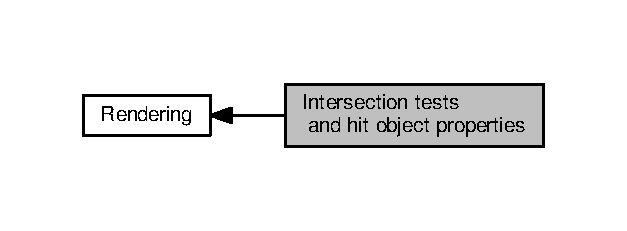
\includegraphics[width=301pt]{group__intersection__test__prperties}
\end{center}
\end{figure}
\subsection*{Functions}
\begin{DoxyCompactItemize}
\item 
\+\_\+\+\_\+host\+\_\+\+\_\+ \+\_\+\+\_\+device\+\_\+\+\_\+ bool \hyperlink{group__intersection__test__prperties_gac9af7cfe676f4df793dea5bc53171161}{intersect\+Mesh} (\hyperlink{class_ray}{Ray} \&ray, \hyperlink{class_dev_object}{Dev\+Object} \&obj, \hyperlink{struct_g_p_u_1_1_rendering_context}{G\+P\+U\+::\+Rendering\+Context} \&ctxt)
\begin{DoxyCompactList}\small\item\em Checks if a ray intersects a mesh. \end{DoxyCompactList}\item 
\+\_\+\+\_\+host\+\_\+\+\_\+ \+\_\+\+\_\+device\+\_\+\+\_\+ bool \hyperlink{group__intersection__test__prperties_ga8c05ac13c3cdd49f7e4fa3948cfa4699}{intersect\+Sphere} (\hyperlink{class_ray}{Ray} \&ray, \hyperlink{class_dev_object}{Dev\+Object} \&obj, \hyperlink{struct_g_p_u_1_1_rendering_context}{G\+P\+U\+::\+Rendering\+Context} \&ctxt)
\begin{DoxyCompactList}\small\item\em Checks if a ray intersects a sphere. \end{DoxyCompactList}\item 
\+\_\+\+\_\+host\+\_\+\+\_\+ \+\_\+\+\_\+device\+\_\+\+\_\+ bool \hyperlink{group__intersection__test__prperties_gafbcfd99d540347f9f63d01d6d0b6eef5}{intersect\+Plane} (\hyperlink{class_ray}{Ray} \&ray, \hyperlink{class_dev_object}{Dev\+Object} \&obj, \hyperlink{struct_g_p_u_1_1_rendering_context}{G\+P\+U\+::\+Rendering\+Context} \&ctxt)
\begin{DoxyCompactList}\small\item\em Checks if a ray intersects a plane. \end{DoxyCompactList}\item 
\+\_\+\+\_\+host\+\_\+\+\_\+ \+\_\+\+\_\+device\+\_\+\+\_\+ bool \hyperlink{group__intersection__test__prperties_gae4778d3b0c160c9757d7fca0e5deefa2}{intersect\+Cube} (\hyperlink{class_ray}{Ray} \&ray, \hyperlink{class_dev_object}{Dev\+Object} \&obj, \hyperlink{struct_g_p_u_1_1_rendering_context}{G\+P\+U\+::\+Rendering\+Context} \&ctxt)
\begin{DoxyCompactList}\small\item\em Checks if a ray intersects a cube. \end{DoxyCompactList}\item 
\+\_\+\+\_\+host\+\_\+\+\_\+ \+\_\+\+\_\+device\+\_\+\+\_\+ bool \hyperlink{group__intersection__test__prperties_gaf6bbee9e8a6ee564017fa94cd9e6ec63}{intersect\+Bounding\+Volume} (\hyperlink{class_ray}{Ray} \&ray, float(\&precompute)\mbox{[}2\mbox{]}\mbox{[}7\mbox{]}, \hyperlink{class_dev_object}{Dev\+Object} \&current\+Object, uint8\+\_\+t \&normal\+Index)
\begin{DoxyCompactList}\small\item\em Checks if a ray intersects a bounding slabs of a triangle mesh. \end{DoxyCompactList}\item 
\+\_\+\+\_\+host\+\_\+\+\_\+ \+\_\+\+\_\+device\+\_\+\+\_\+ void \hyperlink{group__intersection__test__prperties_gaa26e85d7aac46c25d6a1b975423f968d}{mesh\+Properties} (const \hyperlink{class_dev_object}{Dev\+Object} \&object, const \hyperlink{class_vec3}{Vec3f} \&hit\+Point, \hyperlink{struct_g_p_u_1_1_rendering_context}{G\+P\+U\+::\+Rendering\+Context} \&ctx, \hyperlink{class_vec2}{Vec2f} \&hit\+Texture\+Coordinates)
\begin{DoxyCompactList}\small\item\em Gets mesh properties on a hitpoint. \end{DoxyCompactList}\item 
\+\_\+\+\_\+host\+\_\+\+\_\+ \+\_\+\+\_\+device\+\_\+\+\_\+ void \hyperlink{group__intersection__test__prperties_gae821d5671069271f7c39d22ca8950f3d}{sphere\+Properties} (const \hyperlink{class_dev_object}{Dev\+Object} \&object, const \hyperlink{class_vec3}{Vec3f} \&hit\+Point, \hyperlink{struct_g_p_u_1_1_rendering_context}{G\+P\+U\+::\+Rendering\+Context} \&ctx, \hyperlink{class_vec2}{Vec2f} \&hit\+Texture\+Coordinates)
\begin{DoxyCompactList}\small\item\em Gets sphere properties on a hitpoint. \end{DoxyCompactList}\item 
\+\_\+\+\_\+host\+\_\+\+\_\+ \+\_\+\+\_\+device\+\_\+\+\_\+ void \hyperlink{group__intersection__test__prperties_gae25700b3104d615db9d575d086c3d994}{plane\+Properties} (const \hyperlink{class_dev_object}{Dev\+Object} \&object, const \hyperlink{class_vec3}{Vec3f} \&hit\+Point, \hyperlink{struct_g_p_u_1_1_rendering_context}{G\+P\+U\+::\+Rendering\+Context} \&ctx, \hyperlink{class_vec2}{Vec2f} \&hit\+Texture\+Coordinates)
\begin{DoxyCompactList}\small\item\em Gets plane properties on a hitpoint. \end{DoxyCompactList}\item 
\+\_\+\+\_\+host\+\_\+\+\_\+ \+\_\+\+\_\+device\+\_\+\+\_\+ void \hyperlink{group__intersection__test__prperties_ga33e6e14712999e0675085b5479201656}{cube\+Properties} (const \hyperlink{class_dev_object}{Dev\+Object} \&object, const \hyperlink{class_vec3}{Vec3f} \&hit\+Point, \hyperlink{struct_g_p_u_1_1_rendering_context}{G\+P\+U\+::\+Rendering\+Context} \&ctx, \hyperlink{class_vec2}{Vec2f} \&hit\+Texture\+Coordinates)
\begin{DoxyCompactList}\small\item\em Gets cube properties on a hitpoint. \end{DoxyCompactList}\item 
void \hyperlink{group__intersection__test__prperties_gae4e3caaa9b4a37b20a8a6f84d0c326aa}{delete\+Mesh} (\hyperlink{class_dev_object}{Dev\+Object} $\ast$object)
\begin{DoxyCompactList}\small\item\em Device memory deallocation function. \end{DoxyCompactList}\item 
\+\_\+\+\_\+device\+\_\+\+\_\+ void \hyperlink{group__intersection__test__prperties_ga4b2a399a49c34312c8369f54b79230af}{transform\+Mesh} (\hyperlink{class_dev_object}{Dev\+Object} $\ast$object, const \hyperlink{class_square_matrix4}{Square\+Matrix4f} \&m\+Transform)
\begin{DoxyCompactList}\small\item\em Whole mesh translation, rotation and scale function. \end{DoxyCompactList}\item 
\+\_\+\+\_\+device\+\_\+\+\_\+ void \hyperlink{group__intersection__test__prperties_ga6fe7123c4c4bdf775eac1231bc37c490}{transform\+Sphere} (\hyperlink{class_dev_object}{Dev\+Object} $\ast$object, const \hyperlink{class_square_matrix4}{Square\+Matrix4f} \&m\+Transform)
\begin{DoxyCompactList}\small\item\em Implicit sphere translation, rotation and scale function. \end{DoxyCompactList}\item 
\+\_\+\+\_\+device\+\_\+\+\_\+ void \hyperlink{group__intersection__test__prperties_ga6d2ae68047e8f8d11a64b9dc9dda507d}{transform\+Plane} (\hyperlink{class_dev_object}{Dev\+Object} $\ast$object, const \hyperlink{class_square_matrix4}{Square\+Matrix4f} \&m\+Transform)
\begin{DoxyCompactList}\small\item\em Implicit sphere translation, rotation and scale function. \end{DoxyCompactList}\item 
\+\_\+\+\_\+device\+\_\+\+\_\+ void \hyperlink{group__intersection__test__prperties_ga00e56ff810e7ba397e903acf50626b55}{transform\+Cube} (\hyperlink{class_dev_object}{Dev\+Object} $\ast$object, const \hyperlink{class_square_matrix4}{Square\+Matrix4f} \&m\+Transform)
\begin{DoxyCompactList}\small\item\em Implicit sphere translation, rotation and scale function. \end{DoxyCompactList}\item 
\+\_\+\+\_\+device\+\_\+\+\_\+ \hyperlink{class_vec3}{Vec3f} \hyperlink{group__intersection__test__prperties_ga19abb6bc50199d8583aafedd0e044b7e}{distant\+Light\+Reflected\+Color} (const \hyperlink{class_i_light}{I\+Light} $\ast$\+\_\+light, \hyperlink{struct_g_p_u_1_1_rendering_context}{G\+P\+U\+::\+Rendering\+Context} \&rctx, \hyperlink{class_vec3}{Vec3f} \&albedo)
\begin{DoxyCompactList}\small\item\em \hyperlink{struct_appearence}{Appearence} of incident light. \end{DoxyCompactList}\item 
\+\_\+\+\_\+device\+\_\+\+\_\+ void \hyperlink{group__intersection__test__prperties_ga6a438778f6ed8683785d7a892a05d312}{illuminate\+Distant} (const \hyperlink{class_i_light}{I\+Light} \&light, const \hyperlink{class_vec3}{Vec3f} \&P, \hyperlink{class_vec3}{Vec3f} \&light\+Dir, \hyperlink{class_vec3}{Vec3f} \&light\+Intensity, float \&distance)
\begin{DoxyCompactList}\small\item\em Implicit sphere translation, rotation and scale function. \end{DoxyCompactList}\item 
\+\_\+\+\_\+device\+\_\+\+\_\+ void \hyperlink{group__intersection__test__prperties_gab3c663df5b5a29d04083e7793bce50d5}{illuminate\+Point} (const \hyperlink{class_i_light}{I\+Light} \&light, const \hyperlink{class_vec3}{Vec3f} \&P, \hyperlink{class_vec3}{Vec3f} \&light\+Dir, \hyperlink{class_vec3}{Vec3f} \&light\+Intensity, float \&distance)
\begin{DoxyCompactList}\small\item\em Implicit sphere translation, rotation and scale function. \end{DoxyCompactList}\item 
void \hyperlink{group__intersection__test__prperties_ga672ecbee3aea2f5567ad7a2611feef3e}{set\+Mesh\+Acceleration\+Volume} (const \hyperlink{class_dev_object}{Dev\+Object} $\ast$current\+Object, \hyperlink{class_boundaries}{Boundaries} $\ast$boundaries, \hyperlink{class_vec3}{Vec3f}(\&bounding\+Plane\+Normals)\mbox{[}7\mbox{]}, float $\ast$(\&gpu\+\_\+all\+Dot\+Products)\mbox{[}7\mbox{]})
\begin{DoxyCompactList}\small\item\em The function gets bounding volume distances computed. \end{DoxyCompactList}\item 
void \hyperlink{group__intersection__test__prperties_gafd2f15ce4a55fb0d8daee0bff024b67b}{set\+Sphere\+Acceleration\+Volume} (const \hyperlink{class_dev_object}{Dev\+Object} $\ast$current\+Object, \hyperlink{class_boundaries}{Boundaries} $\ast$boundaries, \hyperlink{class_vec3}{Vec3f}(\&bounding\+Plane\+Normals)\mbox{[}7\mbox{]}, float $\ast$(\&gpu\+\_\+all\+Dot\+Products)\mbox{[}7\mbox{]})
\begin{DoxyCompactList}\small\item\em The function gets bounding volume distances computed. \end{DoxyCompactList}\item 
void \hyperlink{group__intersection__test__prperties_ga684f41eb2add27e32a7c0115cdd6cce1}{set\+Plane\+Acceleration\+Volume} (const \hyperlink{class_dev_object}{Dev\+Object} $\ast$current\+Object, \hyperlink{class_boundaries}{Boundaries} $\ast$boundaries, \hyperlink{class_vec3}{Vec3f}(\&bounding\+Plane\+Normals)\mbox{[}7\mbox{]}, float $\ast$(\&gpu\+\_\+all\+Dot\+Products)\mbox{[}7\mbox{]})
\begin{DoxyCompactList}\small\item\em The function gets bounding volume distances computed. \end{DoxyCompactList}\item 
void \hyperlink{group__intersection__test__prperties_gabfac85fdf9d0cceb70aefa4c2ed71ad2}{set\+Cube\+Acceleration\+Volume} (const \hyperlink{class_dev_object}{Dev\+Object} $\ast$current\+Object, \hyperlink{class_boundaries}{Boundaries} $\ast$boundaries, \hyperlink{class_vec3}{Vec3f}(\&bounding\+Plane\+Normals)\mbox{[}7\mbox{]}, float $\ast$(\&gpu\+\_\+all\+Dot\+Products)\mbox{[}7\mbox{]})
\begin{DoxyCompactList}\small\item\em The function gets bounding volume distances computed. \end{DoxyCompactList}\item 
\+\_\+\+\_\+device\+\_\+\+\_\+ float \hyperlink{group__intersection__test__prperties_gae0b690ff7b5f9b93e53bb0c1437fbf55}{strips} (const \hyperlink{class_vec2}{Vec2f} \&hit\+Tex\+Coordinates)
\begin{DoxyCompactList}\small\item\em Computes pattern at a particular point in texture. \end{DoxyCompactList}\item 
\+\_\+\+\_\+device\+\_\+\+\_\+ float \hyperlink{group__intersection__test__prperties_gaff97add1678535636b1f4f1ca3f7a96c}{wave} (const \hyperlink{class_vec2}{Vec2f} \&hit\+Tex\+Coordinates)
\begin{DoxyCompactList}\small\item\em Computes pattern at a particular point in texture. \end{DoxyCompactList}\item 
\+\_\+\+\_\+device\+\_\+\+\_\+ float \hyperlink{group__intersection__test__prperties_ga4db329f1c6b211cd0ac9e6dc297f279e}{grid} (const \hyperlink{class_vec2}{Vec2f} \&hit\+Tex\+Coordinates)
\begin{DoxyCompactList}\small\item\em Computes pattern at a particular point in texture. \end{DoxyCompactList}\item 
\+\_\+\+\_\+device\+\_\+\+\_\+ float \hyperlink{group__intersection__test__prperties_ga100df37360dfe6954f51431bc6343dc6}{checker} (const \hyperlink{class_vec2}{Vec2f} \&hit\+Tex\+Coordinates)
\begin{DoxyCompactList}\small\item\em Computes pattern at a particular point in texture. \end{DoxyCompactList}\item 
\+\_\+\+\_\+device\+\_\+\+\_\+ float \hyperlink{group__intersection__test__prperties_ga6ea9f9e6624268a263962a17c6634feb}{none} (const \hyperlink{class_vec2}{Vec2f} \&hit\+Tex\+Coordinates)
\begin{DoxyCompactList}\small\item\em Function just for capability with pattern calculation. \end{DoxyCompactList}\end{DoxyCompactItemize}


\subsection{Detailed Description}


\subsection{Function Documentation}
\index{Intersection tests and hit object properties@{Intersection tests and hit object properties}!checker@{checker}}
\index{checker@{checker}!Intersection tests and hit object properties@{Intersection tests and hit object properties}}
\subsubsection[{\texorpdfstring{checker(const Vec2f \&hit\+Tex\+Coordinates)}{checker(const Vec2f \&hitTexCoordinates)}}]{\setlength{\rightskip}{0pt plus 5cm}\+\_\+\+\_\+device\+\_\+\+\_\+ float checker (
\begin{DoxyParamCaption}
\item[{const {\bf Vec2f} \&}]{hit\+Tex\+Coordinates}
\end{DoxyParamCaption}
)}\hypertarget{group__intersection__test__prperties_ga100df37360dfe6954f51431bc6343dc6}{}\label{group__intersection__test__prperties_ga100df37360dfe6954f51431bc6343dc6}


Computes pattern at a particular point in texture. 


\begin{DoxyParams}[1]{Parameters}
\mbox{\tt in}  & {\em hit\+Tex\+Coordinates} & \\
\hline
\end{DoxyParams}
\begin{DoxyReturn}{Returns}
a normalized floating point number 
\end{DoxyReturn}
\index{Intersection tests and hit object properties@{Intersection tests and hit object properties}!cube\+Properties@{cube\+Properties}}
\index{cube\+Properties@{cube\+Properties}!Intersection tests and hit object properties@{Intersection tests and hit object properties}}
\subsubsection[{\texorpdfstring{cube\+Properties(const Dev\+Object \&object, const Vec3f \&hit\+Point, G\+P\+U\+::\+Rendering\+Context \&ctx, Vec2f \&hit\+Texture\+Coordinates)}{cubeProperties(const DevObject \&object, const Vec3f \&hitPoint, GPU::RenderingContext \&ctx, Vec2f \&hitTextureCoordinates)}}]{\setlength{\rightskip}{0pt plus 5cm}\+\_\+\+\_\+host\+\_\+\+\_\+ \+\_\+\+\_\+device\+\_\+\+\_\+ void cube\+Properties (
\begin{DoxyParamCaption}
\item[{const {\bf Dev\+Object} \&}]{object, }
\item[{const {\bf Vec3f} \&}]{hit\+Point, }
\item[{{\bf G\+P\+U\+::\+Rendering\+Context} \&}]{ctx, }
\item[{{\bf Vec2f} \&}]{hit\+Texture\+Coordinates}
\end{DoxyParamCaption}
)}\hypertarget{group__intersection__test__prperties_ga33e6e14712999e0675085b5479201656}{}\label{group__intersection__test__prperties_ga33e6e14712999e0675085b5479201656}


Gets cube properties on a hitpoint. 


\begin{DoxyParams}[1]{Parameters}
\mbox{\tt in}  & {\em object} & -\/ wrapper with a specific object\textquotesingle{}s data \\
\hline
\mbox{\tt out}  & {\em hit\+Point} & -\/ output argument to get hit point \\
\hline
\mbox{\tt out}  & {\em ctx} & -\/ output argument to get texture barycentric coordinates \\
\hline
\mbox{\tt out}  & {\em hit\+Texture\+Coordinates} & -\/ texture coordinates with regards to barycentric coordinates of hit point. \\
\hline
\end{DoxyParams}
\index{Intersection tests and hit object properties@{Intersection tests and hit object properties}!delete\+Mesh@{delete\+Mesh}}
\index{delete\+Mesh@{delete\+Mesh}!Intersection tests and hit object properties@{Intersection tests and hit object properties}}
\subsubsection[{\texorpdfstring{delete\+Mesh(\+Dev\+Object $\ast$object)}{deleteMesh(DevObject *object)}}]{\setlength{\rightskip}{0pt plus 5cm}void delete\+Mesh (
\begin{DoxyParamCaption}
\item[{{\bf Dev\+Object} $\ast$}]{object}
\end{DoxyParamCaption}
)}\hypertarget{group__intersection__test__prperties_gae4e3caaa9b4a37b20a8a6f84d0c326aa}{}\label{group__intersection__test__prperties_gae4e3caaa9b4a37b20a8a6f84d0c326aa}


Device memory deallocation function. 


\begin{DoxyParams}[1]{Parameters}
\mbox{\tt out}  & {\em object} & -\/ wrapper with a specific object\textquotesingle{}s data \\
\hline
\end{DoxyParams}
Here is the caller graph for this function\+:
\nopagebreak
\begin{figure}[H]
\begin{center}
\leavevmode
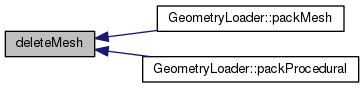
\includegraphics[width=345pt]{group__intersection__test__prperties_gae4e3caaa9b4a37b20a8a6f84d0c326aa_icgraph}
\end{center}
\end{figure}
\index{Intersection tests and hit object properties@{Intersection tests and hit object properties}!distant\+Light\+Reflected\+Color@{distant\+Light\+Reflected\+Color}}
\index{distant\+Light\+Reflected\+Color@{distant\+Light\+Reflected\+Color}!Intersection tests and hit object properties@{Intersection tests and hit object properties}}
\subsubsection[{\texorpdfstring{distant\+Light\+Reflected\+Color(const I\+Light $\ast$\+\_\+light, G\+P\+U\+::\+Rendering\+Context \&rctx, Vec3f \&albedo)}{distantLightReflectedColor(const ILight *\_light, GPU::RenderingContext \&rctx, Vec3f \&albedo)}}]{\setlength{\rightskip}{0pt plus 5cm}\+\_\+\+\_\+device\+\_\+\+\_\+ {\bf Vec3f} distant\+Light\+Reflected\+Color (
\begin{DoxyParamCaption}
\item[{const {\bf I\+Light} $\ast$}]{\+\_\+light, }
\item[{{\bf G\+P\+U\+::\+Rendering\+Context} \&}]{rctx, }
\item[{{\bf Vec3f} \&}]{albedo}
\end{DoxyParamCaption}
)}\hypertarget{group__intersection__test__prperties_ga19abb6bc50199d8583aafedd0e044b7e}{}\label{group__intersection__test__prperties_ga19abb6bc50199d8583aafedd0e044b7e}


\hyperlink{struct_appearence}{Appearence} of incident light. 


\begin{DoxyParams}[1]{Parameters}
\mbox{\tt in}  & {\em \+\_\+light} & -\/ wrapper with a specific light\textquotesingle{}s data \\
\hline
\mbox{\tt in}  & {\em rctx} & \\
\hline
\mbox{\tt in}  & {\em albedo} & \\
\hline
\end{DoxyParams}
Here is the call graph for this function\+:
\nopagebreak
\begin{figure}[H]
\begin{center}
\leavevmode
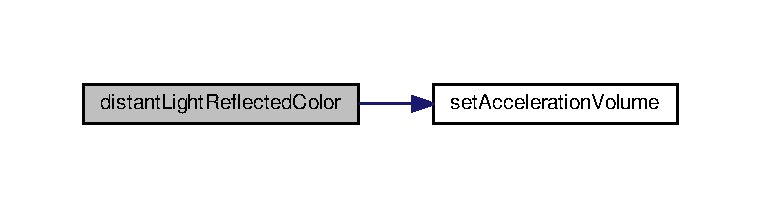
\includegraphics[width=350pt]{group__intersection__test__prperties_ga19abb6bc50199d8583aafedd0e044b7e_cgraph}
\end{center}
\end{figure}
\index{Intersection tests and hit object properties@{Intersection tests and hit object properties}!grid@{grid}}
\index{grid@{grid}!Intersection tests and hit object properties@{Intersection tests and hit object properties}}
\subsubsection[{\texorpdfstring{grid(const Vec2f \&hit\+Tex\+Coordinates)}{grid(const Vec2f \&hitTexCoordinates)}}]{\setlength{\rightskip}{0pt plus 5cm}\+\_\+\+\_\+device\+\_\+\+\_\+ float grid (
\begin{DoxyParamCaption}
\item[{const {\bf Vec2f} \&}]{hit\+Tex\+Coordinates}
\end{DoxyParamCaption}
)}\hypertarget{group__intersection__test__prperties_ga4db329f1c6b211cd0ac9e6dc297f279e}{}\label{group__intersection__test__prperties_ga4db329f1c6b211cd0ac9e6dc297f279e}


Computes pattern at a particular point in texture. 


\begin{DoxyParams}[1]{Parameters}
\mbox{\tt in}  & {\em hit\+Tex\+Coordinates} & \\
\hline
\end{DoxyParams}
\begin{DoxyReturn}{Returns}
a normalized floating point number 
\end{DoxyReturn}
\index{Intersection tests and hit object properties@{Intersection tests and hit object properties}!illuminate\+Distant@{illuminate\+Distant}}
\index{illuminate\+Distant@{illuminate\+Distant}!Intersection tests and hit object properties@{Intersection tests and hit object properties}}
\subsubsection[{\texorpdfstring{illuminate\+Distant(const I\+Light \&light, const Vec3f \&\+P, Vec3f \&light\+Dir, Vec3f \&light\+Intensity, float \&distance)}{illuminateDistant(const ILight \&light, const Vec3f \&P, Vec3f \&lightDir, Vec3f \&lightIntensity, float \&distance)}}]{\setlength{\rightskip}{0pt plus 5cm}\+\_\+\+\_\+device\+\_\+\+\_\+ void illuminate\+Distant (
\begin{DoxyParamCaption}
\item[{const {\bf I\+Light} \&}]{light, }
\item[{const {\bf Vec3f} \&}]{P, }
\item[{{\bf Vec3f} \&}]{light\+Dir, }
\item[{{\bf Vec3f} \&}]{light\+Intensity, }
\item[{float \&}]{distance}
\end{DoxyParamCaption}
)}\hypertarget{group__intersection__test__prperties_ga6a438778f6ed8683785d7a892a05d312}{}\label{group__intersection__test__prperties_ga6a438778f6ed8683785d7a892a05d312}


Implicit sphere translation, rotation and scale function. 


\begin{DoxyParams}[1]{Parameters}
\mbox{\tt in}  & {\em light} & -\/ wrapper with a specific light\textquotesingle{}s data \\
\hline
\mbox{\tt in}  & {\em P} & -\/ not used here \\
\hline
\mbox{\tt in}  & {\em light\+Dir} & -\/ light direction. \\
\hline
\mbox{\tt in}  & {\em light\+Intensity} & \\
\hline
\mbox{\tt in}  & {\em distance} & -\/ not used here. \\
\hline
\end{DoxyParams}
\index{Intersection tests and hit object properties@{Intersection tests and hit object properties}!illuminate\+Point@{illuminate\+Point}}
\index{illuminate\+Point@{illuminate\+Point}!Intersection tests and hit object properties@{Intersection tests and hit object properties}}
\subsubsection[{\texorpdfstring{illuminate\+Point(const I\+Light \&light, const Vec3f \&\+P, Vec3f \&light\+Dir, Vec3f \&light\+Intensity, float \&distance)}{illuminatePoint(const ILight \&light, const Vec3f \&P, Vec3f \&lightDir, Vec3f \&lightIntensity, float \&distance)}}]{\setlength{\rightskip}{0pt plus 5cm}\+\_\+\+\_\+device\+\_\+\+\_\+ void illuminate\+Point (
\begin{DoxyParamCaption}
\item[{const {\bf I\+Light} \&}]{light, }
\item[{const {\bf Vec3f} \&}]{P, }
\item[{{\bf Vec3f} \&}]{light\+Dir, }
\item[{{\bf Vec3f} \&}]{light\+Intensity, }
\item[{float \&}]{distance}
\end{DoxyParamCaption}
)}\hypertarget{group__intersection__test__prperties_gab3c663df5b5a29d04083e7793bce50d5}{}\label{group__intersection__test__prperties_gab3c663df5b5a29d04083e7793bce50d5}


Implicit sphere translation, rotation and scale function. 


\begin{DoxyParams}[1]{Parameters}
\mbox{\tt in}  & {\em light} & -\/ wrapper with a specific light\textquotesingle{}s data \\
\hline
\mbox{\tt in}  & {\em P} & -\/ light source position. \\
\hline
\mbox{\tt out}  & {\em light\+Dir} & -\/ light direction. \\
\hline
\mbox{\tt out}  & {\em light\+Intensity} & \\
\hline
\mbox{\tt out}  & {\em distance} & -\/ distance to light source \\
\hline
\end{DoxyParams}
\index{Intersection tests and hit object properties@{Intersection tests and hit object properties}!intersect\+Bounding\+Volume@{intersect\+Bounding\+Volume}}
\index{intersect\+Bounding\+Volume@{intersect\+Bounding\+Volume}!Intersection tests and hit object properties@{Intersection tests and hit object properties}}
\subsubsection[{\texorpdfstring{intersect\+Bounding\+Volume(\+Ray \&ray, float(\&precompute)[2][7], Dev\+Object \&current\+Object, uint8\+\_\+t \&normal\+Index)}{intersectBoundingVolume(Ray \&ray, float(\&precompute)[2][7], DevObject \&currentObject, uint8\_t \&normalIndex)}}]{\setlength{\rightskip}{0pt plus 5cm}\+\_\+\+\_\+host\+\_\+\+\_\+ \+\_\+\+\_\+device\+\_\+\+\_\+ bool intersect\+Bounding\+Volume (
\begin{DoxyParamCaption}
\item[{{\bf Ray} \&}]{ray, }
\item[{float(\&)}]{precompute\mbox{[}2\mbox{]}\mbox{[}7\mbox{]}, }
\item[{{\bf Dev\+Object} \&}]{current\+Object, }
\item[{uint8\+\_\+t \&}]{normal\+Index}
\end{DoxyParamCaption}
)}\hypertarget{group__intersection__test__prperties_gaf6bbee9e8a6ee564017fa94cd9e6ec63}{}\label{group__intersection__test__prperties_gaf6bbee9e8a6ee564017fa94cd9e6ec63}


Checks if a ray intersects a bounding slabs of a triangle mesh. 


\begin{DoxyParams}[1]{Parameters}
\mbox{\tt in}  & {\em ray} & -\/ the ray structure \\
\hline
\mbox{\tt out}  & {\em precompute} & -\/ a precomputed( in Object\+Box\+::hit ) array of dot products divisions \\
\hline
\mbox{\tt out}  & {\em current\+Object} & wrapper with a specific object\textquotesingle{}s data \\
\hline
\mbox{\tt out}  & {\em normal\+Index} & -\/ needed to get a normal of a slab. \\
\hline
\end{DoxyParams}
Here is the call graph for this function\+:
\nopagebreak
\begin{figure}[H]
\begin{center}
\leavevmode
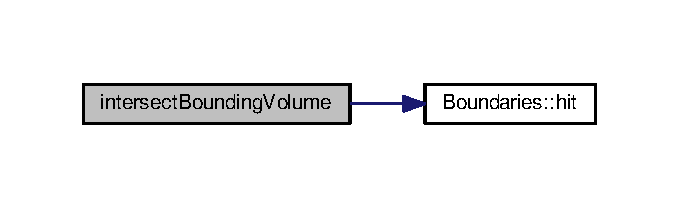
\includegraphics[width=326pt]{group__intersection__test__prperties_gaf6bbee9e8a6ee564017fa94cd9e6ec63_cgraph}
\end{center}
\end{figure}
\index{Intersection tests and hit object properties@{Intersection tests and hit object properties}!intersect\+Cube@{intersect\+Cube}}
\index{intersect\+Cube@{intersect\+Cube}!Intersection tests and hit object properties@{Intersection tests and hit object properties}}
\subsubsection[{\texorpdfstring{intersect\+Cube(\+Ray \&ray, Dev\+Object \&obj, G\+P\+U\+::\+Rendering\+Context \&ctxt)}{intersectCube(Ray \&ray, DevObject \&obj, GPU::RenderingContext \&ctxt)}}]{\setlength{\rightskip}{0pt plus 5cm}\+\_\+\+\_\+host\+\_\+\+\_\+ \+\_\+\+\_\+device\+\_\+\+\_\+ bool intersect\+Cube (
\begin{DoxyParamCaption}
\item[{{\bf Ray} \&}]{ray, }
\item[{{\bf Dev\+Object} \&}]{obj, }
\item[{{\bf G\+P\+U\+::\+Rendering\+Context} \&}]{ctxt}
\end{DoxyParamCaption}
)}\hypertarget{group__intersection__test__prperties_gae4778d3b0c160c9757d7fca0e5deefa2}{}\label{group__intersection__test__prperties_gae4778d3b0c160c9757d7fca0e5deefa2}


Checks if a ray intersects a cube. 


\begin{DoxyParams}[1]{Parameters}
\mbox{\tt in}  & {\em ray} & -\/ the ray structure \\
\hline
\mbox{\tt out}  & {\em obj} & -\/ wrapper with a specific object\textquotesingle{}s data \\
\hline
\mbox{\tt out}  & {\em ctxt} & -\/ structure gets texture coordinates etc. \\
\hline
\end{DoxyParams}
Here is the call graph for this function\+:
\nopagebreak
\begin{figure}[H]
\begin{center}
\leavevmode
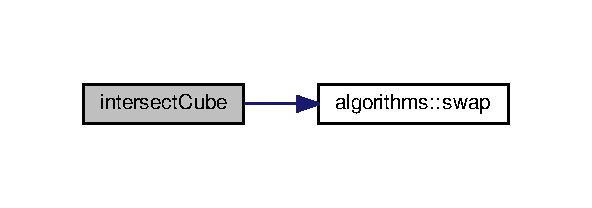
\includegraphics[width=284pt]{group__intersection__test__prperties_gae4778d3b0c160c9757d7fca0e5deefa2_cgraph}
\end{center}
\end{figure}
\index{Intersection tests and hit object properties@{Intersection tests and hit object properties}!intersect\+Mesh@{intersect\+Mesh}}
\index{intersect\+Mesh@{intersect\+Mesh}!Intersection tests and hit object properties@{Intersection tests and hit object properties}}
\subsubsection[{\texorpdfstring{intersect\+Mesh(\+Ray \&ray, Dev\+Object \&obj, G\+P\+U\+::\+Rendering\+Context \&ctxt)}{intersectMesh(Ray \&ray, DevObject \&obj, GPU::RenderingContext \&ctxt)}}]{\setlength{\rightskip}{0pt plus 5cm}\+\_\+\+\_\+host\+\_\+\+\_\+ \+\_\+\+\_\+device\+\_\+\+\_\+ bool intersect\+Mesh (
\begin{DoxyParamCaption}
\item[{{\bf Ray} \&}]{ray, }
\item[{{\bf Dev\+Object} \&}]{obj, }
\item[{{\bf G\+P\+U\+::\+Rendering\+Context} \&}]{ctxt}
\end{DoxyParamCaption}
)}\hypertarget{group__intersection__test__prperties_gac9af7cfe676f4df793dea5bc53171161}{}\label{group__intersection__test__prperties_gac9af7cfe676f4df793dea5bc53171161}


Checks if a ray intersects a mesh. 


\begin{DoxyParams}[1]{Parameters}
\mbox{\tt out}  & {\em ray} & -\/ the ray structure \\
\hline
\mbox{\tt out}  & {\em obj} & wrapper with a specific object\textquotesingle{}s data \\
\hline
\mbox{\tt out}  & {\em ctxt} & structure gets texture coordinates etc. \\
\hline
\end{DoxyParams}
\index{Intersection tests and hit object properties@{Intersection tests and hit object properties}!intersect\+Plane@{intersect\+Plane}}
\index{intersect\+Plane@{intersect\+Plane}!Intersection tests and hit object properties@{Intersection tests and hit object properties}}
\subsubsection[{\texorpdfstring{intersect\+Plane(\+Ray \&ray, Dev\+Object \&obj, G\+P\+U\+::\+Rendering\+Context \&ctxt)}{intersectPlane(Ray \&ray, DevObject \&obj, GPU::RenderingContext \&ctxt)}}]{\setlength{\rightskip}{0pt plus 5cm}\+\_\+\+\_\+host\+\_\+\+\_\+ \+\_\+\+\_\+device\+\_\+\+\_\+ bool intersect\+Plane (
\begin{DoxyParamCaption}
\item[{{\bf Ray} \&}]{ray, }
\item[{{\bf Dev\+Object} \&}]{obj, }
\item[{{\bf G\+P\+U\+::\+Rendering\+Context} \&}]{ctxt}
\end{DoxyParamCaption}
)}\hypertarget{group__intersection__test__prperties_gafbcfd99d540347f9f63d01d6d0b6eef5}{}\label{group__intersection__test__prperties_gafbcfd99d540347f9f63d01d6d0b6eef5}


Checks if a ray intersects a plane. 


\begin{DoxyParams}[1]{Parameters}
\mbox{\tt in}  & {\em ray} & -\/ the ray structure \\
\hline
\mbox{\tt out}  & {\em obj} & -\/ wrapper with a specific object\textquotesingle{}s data \\
\hline
\mbox{\tt out}  & {\em ctxt} & -\/ structure gets texture coordinates etc. \\
\hline
\end{DoxyParams}
\index{Intersection tests and hit object properties@{Intersection tests and hit object properties}!intersect\+Sphere@{intersect\+Sphere}}
\index{intersect\+Sphere@{intersect\+Sphere}!Intersection tests and hit object properties@{Intersection tests and hit object properties}}
\subsubsection[{\texorpdfstring{intersect\+Sphere(\+Ray \&ray, Dev\+Object \&obj, G\+P\+U\+::\+Rendering\+Context \&ctxt)}{intersectSphere(Ray \&ray, DevObject \&obj, GPU::RenderingContext \&ctxt)}}]{\setlength{\rightskip}{0pt plus 5cm}\+\_\+\+\_\+host\+\_\+\+\_\+ \+\_\+\+\_\+device\+\_\+\+\_\+ bool intersect\+Sphere (
\begin{DoxyParamCaption}
\item[{{\bf Ray} \&}]{ray, }
\item[{{\bf Dev\+Object} \&}]{obj, }
\item[{{\bf G\+P\+U\+::\+Rendering\+Context} \&}]{ctxt}
\end{DoxyParamCaption}
)}\hypertarget{group__intersection__test__prperties_ga8c05ac13c3cdd49f7e4fa3948cfa4699}{}\label{group__intersection__test__prperties_ga8c05ac13c3cdd49f7e4fa3948cfa4699}


Checks if a ray intersects a sphere. 


\begin{DoxyParams}[1]{Parameters}
\mbox{\tt in}  & {\em ray} & -\/ the ray structure \\
\hline
\mbox{\tt out}  & {\em obj} & -\/ wrapper with a specific object\textquotesingle{}s data \\
\hline
\mbox{\tt out}  & {\em ctxt} & -\/ structure gets texture coordinates etc. \\
\hline
\end{DoxyParams}
Here is the call graph for this function\+:
\nopagebreak
\begin{figure}[H]
\begin{center}
\leavevmode
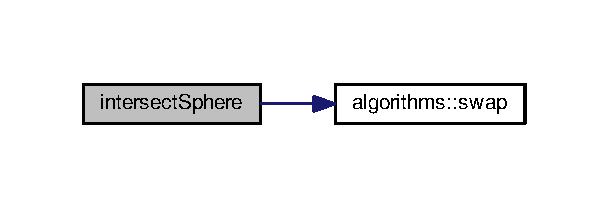
\includegraphics[width=292pt]{group__intersection__test__prperties_ga8c05ac13c3cdd49f7e4fa3948cfa4699_cgraph}
\end{center}
\end{figure}
\index{Intersection tests and hit object properties@{Intersection tests and hit object properties}!mesh\+Properties@{mesh\+Properties}}
\index{mesh\+Properties@{mesh\+Properties}!Intersection tests and hit object properties@{Intersection tests and hit object properties}}
\subsubsection[{\texorpdfstring{mesh\+Properties(const Dev\+Object \&object, const Vec3f \&hit\+Point, G\+P\+U\+::\+Rendering\+Context \&ctx, Vec2f \&hit\+Texture\+Coordinates)}{meshProperties(const DevObject \&object, const Vec3f \&hitPoint, GPU::RenderingContext \&ctx, Vec2f \&hitTextureCoordinates)}}]{\setlength{\rightskip}{0pt plus 5cm}\+\_\+\+\_\+host\+\_\+\+\_\+ \+\_\+\+\_\+device\+\_\+\+\_\+ void mesh\+Properties (
\begin{DoxyParamCaption}
\item[{const {\bf Dev\+Object} \&}]{object, }
\item[{const {\bf Vec3f} \&}]{hit\+Point, }
\item[{{\bf G\+P\+U\+::\+Rendering\+Context} \&}]{ctx, }
\item[{{\bf Vec2f} \&}]{hit\+Texture\+Coordinates}
\end{DoxyParamCaption}
)}\hypertarget{group__intersection__test__prperties_gaa26e85d7aac46c25d6a1b975423f968d}{}\label{group__intersection__test__prperties_gaa26e85d7aac46c25d6a1b975423f968d}


Gets mesh properties on a hitpoint. 


\begin{DoxyParams}[1]{Parameters}
\mbox{\tt in}  & {\em object} & -\/ wrapper with a specific object\textquotesingle{}s data \\
\hline
\mbox{\tt out}  & {\em hit\+Point} & -\/ output argument to get hit point \\
\hline
\mbox{\tt out}  & {\em ctx} & -\/ output argument to get texture barycentric coordinates \\
\hline
\mbox{\tt out}  & {\em hit\+Texture\+Coordinates} & -\/ texture coordinates with regards to barycentric coordinates of hit point. \\
\hline
\end{DoxyParams}
\index{Intersection tests and hit object properties@{Intersection tests and hit object properties}!none@{none}}
\index{none@{none}!Intersection tests and hit object properties@{Intersection tests and hit object properties}}
\subsubsection[{\texorpdfstring{none(const Vec2f \&hit\+Tex\+Coordinates)}{none(const Vec2f \&hitTexCoordinates)}}]{\setlength{\rightskip}{0pt plus 5cm}\+\_\+\+\_\+device\+\_\+\+\_\+ float none (
\begin{DoxyParamCaption}
\item[{const {\bf Vec2f} \&}]{hit\+Tex\+Coordinates}
\end{DoxyParamCaption}
)}\hypertarget{group__intersection__test__prperties_ga6ea9f9e6624268a263962a17c6634feb}{}\label{group__intersection__test__prperties_ga6ea9f9e6624268a263962a17c6634feb}


Function just for capability with pattern calculation. 


\begin{DoxyParams}[1]{Parameters}
\mbox{\tt in}  & {\em hit\+Tex\+Coordinates} & \\
\hline
\end{DoxyParams}
\begin{DoxyReturn}{Returns}
zero or one 
\end{DoxyReturn}
\index{Intersection tests and hit object properties@{Intersection tests and hit object properties}!plane\+Properties@{plane\+Properties}}
\index{plane\+Properties@{plane\+Properties}!Intersection tests and hit object properties@{Intersection tests and hit object properties}}
\subsubsection[{\texorpdfstring{plane\+Properties(const Dev\+Object \&object, const Vec3f \&hit\+Point, G\+P\+U\+::\+Rendering\+Context \&ctx, Vec2f \&hit\+Texture\+Coordinates)}{planeProperties(const DevObject \&object, const Vec3f \&hitPoint, GPU::RenderingContext \&ctx, Vec2f \&hitTextureCoordinates)}}]{\setlength{\rightskip}{0pt plus 5cm}\+\_\+\+\_\+host\+\_\+\+\_\+ \+\_\+\+\_\+device\+\_\+\+\_\+ void plane\+Properties (
\begin{DoxyParamCaption}
\item[{const {\bf Dev\+Object} \&}]{object, }
\item[{const {\bf Vec3f} \&}]{hit\+Point, }
\item[{{\bf G\+P\+U\+::\+Rendering\+Context} \&}]{ctx, }
\item[{{\bf Vec2f} \&}]{hit\+Texture\+Coordinates}
\end{DoxyParamCaption}
)}\hypertarget{group__intersection__test__prperties_gae25700b3104d615db9d575d086c3d994}{}\label{group__intersection__test__prperties_gae25700b3104d615db9d575d086c3d994}


Gets plane properties on a hitpoint. 


\begin{DoxyParams}[1]{Parameters}
\mbox{\tt in}  & {\em object} & -\/ wrapper with a specific object\textquotesingle{}s data \\
\hline
\mbox{\tt out}  & {\em hit\+Point} & -\/ output argument to get hit point \\
\hline
\mbox{\tt out}  & {\em ctx} & -\/ output argument to get texture barycentric coordinates \\
\hline
\mbox{\tt out}  & {\em hit\+Texture\+Coordinates} & -\/ texture coordinates with regards to barycentric coordinates of hit point. \\
\hline
\end{DoxyParams}
\index{Intersection tests and hit object properties@{Intersection tests and hit object properties}!set\+Cube\+Acceleration\+Volume@{set\+Cube\+Acceleration\+Volume}}
\index{set\+Cube\+Acceleration\+Volume@{set\+Cube\+Acceleration\+Volume}!Intersection tests and hit object properties@{Intersection tests and hit object properties}}
\subsubsection[{\texorpdfstring{set\+Cube\+Acceleration\+Volume(const Dev\+Object $\ast$current\+Object, Boundaries $\ast$boundaries, Vec3f(\&bounding\+Plane\+Normals)[7], float $\ast$(\&gpu\+\_\+all\+Dot\+Products)[7])}{setCubeAccelerationVolume(const DevObject *currentObject, Boundaries *boundaries, Vec3f(\&boundingPlaneNormals)[7], float *(\&gpu\_allDotProducts)[7])}}]{\setlength{\rightskip}{0pt plus 5cm}void set\+Cube\+Acceleration\+Volume (
\begin{DoxyParamCaption}
\item[{const {\bf Dev\+Object} $\ast$}]{current\+Object, }
\item[{{\bf Boundaries} $\ast$}]{boundaries, }
\item[{{\bf Vec3f}(\&)}]{bounding\+Plane\+Normals\mbox{[}7\mbox{]}, }
\item[{float $\ast$(\&)}]{gpu\+\_\+all\+Dot\+Products\mbox{[}7\mbox{]}}
\end{DoxyParamCaption}
)}\hypertarget{group__intersection__test__prperties_gabfac85fdf9d0cceb70aefa4c2ed71ad2}{}\label{group__intersection__test__prperties_gabfac85fdf9d0cceb70aefa4c2ed71ad2}


The function gets bounding volume distances computed. 


\begin{DoxyParams}[1]{Parameters}
\mbox{\tt in}  & {\em object} & -\/ wrapper object with pointer to the stored in device memory specific instance. \\
\hline
\mbox{\tt out}  & {\em boundaries} & -\/ to store result \\
\hline
\mbox{\tt in}  & {\em bounding\+Plane\+Normals} & -\/ bounding plane orientation normals. \\
\hline
\mbox{\tt out}  & {\em gpu\+\_\+all\+Dot\+Products} & -\/ allocated in advance device memory to store all possible distances the function uses. \\
\hline
\end{DoxyParams}
\index{Intersection tests and hit object properties@{Intersection tests and hit object properties}!set\+Mesh\+Acceleration\+Volume@{set\+Mesh\+Acceleration\+Volume}}
\index{set\+Mesh\+Acceleration\+Volume@{set\+Mesh\+Acceleration\+Volume}!Intersection tests and hit object properties@{Intersection tests and hit object properties}}
\subsubsection[{\texorpdfstring{set\+Mesh\+Acceleration\+Volume(const Dev\+Object $\ast$current\+Object, Boundaries $\ast$boundaries, Vec3f(\&bounding\+Plane\+Normals)[7], float $\ast$(\&gpu\+\_\+all\+Dot\+Products)[7])}{setMeshAccelerationVolume(const DevObject *currentObject, Boundaries *boundaries, Vec3f(\&boundingPlaneNormals)[7], float *(\&gpu\_allDotProducts)[7])}}]{\setlength{\rightskip}{0pt plus 5cm}void set\+Mesh\+Acceleration\+Volume (
\begin{DoxyParamCaption}
\item[{const {\bf Dev\+Object} $\ast$}]{current\+Object, }
\item[{{\bf Boundaries} $\ast$}]{boundaries, }
\item[{{\bf Vec3f}(\&)}]{bounding\+Plane\+Normals\mbox{[}7\mbox{]}, }
\item[{float $\ast$(\&)}]{gpu\+\_\+all\+Dot\+Products\mbox{[}7\mbox{]}}
\end{DoxyParamCaption}
)}\hypertarget{group__intersection__test__prperties_ga672ecbee3aea2f5567ad7a2611feef3e}{}\label{group__intersection__test__prperties_ga672ecbee3aea2f5567ad7a2611feef3e}


The function gets bounding volume distances computed. 


\begin{DoxyParams}[1]{Parameters}
\mbox{\tt in}  & {\em current\+Object} & -\/ wrapper object with pointer to the stored in device memory specific instance. \\
\hline
\mbox{\tt out}  & {\em boundaries} & -\/ to store result \\
\hline
\mbox{\tt in}  & {\em bounding\+Plane\+Normals} & -\/ bounding plane orientation normals. \\
\hline
\mbox{\tt out}  & {\em gpu\+\_\+all\+Dot\+Products} & -\/ allocated in advance device memory to store all possible distances the function uses. \\
\hline
\end{DoxyParams}
\index{Intersection tests and hit object properties@{Intersection tests and hit object properties}!set\+Plane\+Acceleration\+Volume@{set\+Plane\+Acceleration\+Volume}}
\index{set\+Plane\+Acceleration\+Volume@{set\+Plane\+Acceleration\+Volume}!Intersection tests and hit object properties@{Intersection tests and hit object properties}}
\subsubsection[{\texorpdfstring{set\+Plane\+Acceleration\+Volume(const Dev\+Object $\ast$current\+Object, Boundaries $\ast$boundaries, Vec3f(\&bounding\+Plane\+Normals)[7], float $\ast$(\&gpu\+\_\+all\+Dot\+Products)[7])}{setPlaneAccelerationVolume(const DevObject *currentObject, Boundaries *boundaries, Vec3f(\&boundingPlaneNormals)[7], float *(\&gpu\_allDotProducts)[7])}}]{\setlength{\rightskip}{0pt plus 5cm}void set\+Plane\+Acceleration\+Volume (
\begin{DoxyParamCaption}
\item[{const {\bf Dev\+Object} $\ast$}]{current\+Object, }
\item[{{\bf Boundaries} $\ast$}]{boundaries, }
\item[{{\bf Vec3f}(\&)}]{bounding\+Plane\+Normals\mbox{[}7\mbox{]}, }
\item[{float $\ast$(\&)}]{gpu\+\_\+all\+Dot\+Products\mbox{[}7\mbox{]}}
\end{DoxyParamCaption}
)}\hypertarget{group__intersection__test__prperties_ga684f41eb2add27e32a7c0115cdd6cce1}{}\label{group__intersection__test__prperties_ga684f41eb2add27e32a7c0115cdd6cce1}


The function gets bounding volume distances computed. 


\begin{DoxyParams}[1]{Parameters}
\mbox{\tt in}  & {\em object} & -\/ wrapper object with pointer to the stored in device memory specific instance. \\
\hline
\mbox{\tt out}  & {\em boundaries} & -\/ to store result \\
\hline
\mbox{\tt in}  & {\em bounding\+Plane\+Normals} & -\/ bounding plane orientation normals. \\
\hline
\mbox{\tt out}  & {\em gpu\+\_\+all\+Dot\+Products} & -\/ allocated in advance device memory to store all possible distances the function uses. \\
\hline
\end{DoxyParams}
\index{Intersection tests and hit object properties@{Intersection tests and hit object properties}!set\+Sphere\+Acceleration\+Volume@{set\+Sphere\+Acceleration\+Volume}}
\index{set\+Sphere\+Acceleration\+Volume@{set\+Sphere\+Acceleration\+Volume}!Intersection tests and hit object properties@{Intersection tests and hit object properties}}
\subsubsection[{\texorpdfstring{set\+Sphere\+Acceleration\+Volume(const Dev\+Object $\ast$current\+Object, Boundaries $\ast$boundaries, Vec3f(\&bounding\+Plane\+Normals)[7], float $\ast$(\&gpu\+\_\+all\+Dot\+Products)[7])}{setSphereAccelerationVolume(const DevObject *currentObject, Boundaries *boundaries, Vec3f(\&boundingPlaneNormals)[7], float *(\&gpu\_allDotProducts)[7])}}]{\setlength{\rightskip}{0pt plus 5cm}void set\+Sphere\+Acceleration\+Volume (
\begin{DoxyParamCaption}
\item[{const {\bf Dev\+Object} $\ast$}]{current\+Object, }
\item[{{\bf Boundaries} $\ast$}]{boundaries, }
\item[{{\bf Vec3f}(\&)}]{bounding\+Plane\+Normals\mbox{[}7\mbox{]}, }
\item[{float $\ast$(\&)}]{gpu\+\_\+all\+Dot\+Products\mbox{[}7\mbox{]}}
\end{DoxyParamCaption}
)}\hypertarget{group__intersection__test__prperties_gafd2f15ce4a55fb0d8daee0bff024b67b}{}\label{group__intersection__test__prperties_gafd2f15ce4a55fb0d8daee0bff024b67b}


The function gets bounding volume distances computed. 


\begin{DoxyParams}[1]{Parameters}
\mbox{\tt in}  & {\em current\+Object} & -\/ wrapper object with pointer to the stored in device memory specific instance. \\
\hline
\mbox{\tt out}  & {\em boundaries} & -\/ to store result \\
\hline
\end{DoxyParams}
\begin{DoxyWarning}{Warning}
Parameters down bellow are not used in this function\+: 
\end{DoxyWarning}

\begin{DoxyParams}{Parameters}
{\em bounding\+Plane\+Normals} & \\
\hline
{\em gpu\+\_\+all\+Dot\+Products} & \\
\hline
\end{DoxyParams}
\index{Intersection tests and hit object properties@{Intersection tests and hit object properties}!sphere\+Properties@{sphere\+Properties}}
\index{sphere\+Properties@{sphere\+Properties}!Intersection tests and hit object properties@{Intersection tests and hit object properties}}
\subsubsection[{\texorpdfstring{sphere\+Properties(const Dev\+Object \&object, const Vec3f \&hit\+Point, G\+P\+U\+::\+Rendering\+Context \&ctx, Vec2f \&hit\+Texture\+Coordinates)}{sphereProperties(const DevObject \&object, const Vec3f \&hitPoint, GPU::RenderingContext \&ctx, Vec2f \&hitTextureCoordinates)}}]{\setlength{\rightskip}{0pt plus 5cm}\+\_\+\+\_\+host\+\_\+\+\_\+ \+\_\+\+\_\+device\+\_\+\+\_\+ void sphere\+Properties (
\begin{DoxyParamCaption}
\item[{const {\bf Dev\+Object} \&}]{object, }
\item[{const {\bf Vec3f} \&}]{hit\+Point, }
\item[{{\bf G\+P\+U\+::\+Rendering\+Context} \&}]{ctx, }
\item[{{\bf Vec2f} \&}]{hit\+Texture\+Coordinates}
\end{DoxyParamCaption}
)}\hypertarget{group__intersection__test__prperties_gae821d5671069271f7c39d22ca8950f3d}{}\label{group__intersection__test__prperties_gae821d5671069271f7c39d22ca8950f3d}


Gets sphere properties on a hitpoint. 


\begin{DoxyParams}[1]{Parameters}
\mbox{\tt in}  & {\em object} & -\/ wrapper with a specific object\textquotesingle{}s data \\
\hline
\mbox{\tt out}  & {\em hit\+Point} & -\/ output argument to get hit point \\
\hline
\mbox{\tt out}  & {\em ctx} & -\/ output argument to get texture barycentric coordinates \\
\hline
\mbox{\tt out}  & {\em hit\+Texture\+Coordinates} & -\/ texture coordinates with regards to barycentric coordinates of hit point. \\
\hline
\end{DoxyParams}
\index{Intersection tests and hit object properties@{Intersection tests and hit object properties}!strips@{strips}}
\index{strips@{strips}!Intersection tests and hit object properties@{Intersection tests and hit object properties}}
\subsubsection[{\texorpdfstring{strips(const Vec2f \&hit\+Tex\+Coordinates)}{strips(const Vec2f \&hitTexCoordinates)}}]{\setlength{\rightskip}{0pt plus 5cm}\+\_\+\+\_\+device\+\_\+\+\_\+ float strips (
\begin{DoxyParamCaption}
\item[{const {\bf Vec2f} \&}]{hit\+Tex\+Coordinates}
\end{DoxyParamCaption}
)}\hypertarget{group__intersection__test__prperties_gae0b690ff7b5f9b93e53bb0c1437fbf55}{}\label{group__intersection__test__prperties_gae0b690ff7b5f9b93e53bb0c1437fbf55}


Computes pattern at a particular point in texture. 


\begin{DoxyParams}[1]{Parameters}
\mbox{\tt in}  & {\em hit\+Tex\+Coordinates} & \\
\hline
\end{DoxyParams}
\index{Intersection tests and hit object properties@{Intersection tests and hit object properties}!transform\+Cube@{transform\+Cube}}
\index{transform\+Cube@{transform\+Cube}!Intersection tests and hit object properties@{Intersection tests and hit object properties}}
\subsubsection[{\texorpdfstring{transform\+Cube(\+Dev\+Object $\ast$object, const Square\+Matrix4f \&m\+Transform)}{transformCube(DevObject *object, const SquareMatrix4f \&mTransform)}}]{\setlength{\rightskip}{0pt plus 5cm}\+\_\+\+\_\+device\+\_\+\+\_\+ void transform\+Cube (
\begin{DoxyParamCaption}
\item[{{\bf Dev\+Object} $\ast$}]{object, }
\item[{const {\bf Square\+Matrix4f} \&}]{m\+Transform}
\end{DoxyParamCaption}
)}\hypertarget{group__intersection__test__prperties_ga00e56ff810e7ba397e903acf50626b55}{}\label{group__intersection__test__prperties_ga00e56ff810e7ba397e903acf50626b55}


Implicit sphere translation, rotation and scale function. 


\begin{DoxyParams}[1]{Parameters}
\mbox{\tt out}  & {\em object} & -\/ wrapper with a specific object\textquotesingle{}s data \\
\hline
\mbox{\tt in}  & {\em m\+Transform} & -\/ object-\/to-\/world matrix \\
\hline
\end{DoxyParams}
Here is the call graph for this function\+:
\nopagebreak
\begin{figure}[H]
\begin{center}
\leavevmode
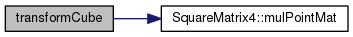
\includegraphics[width=337pt]{group__intersection__test__prperties_ga00e56ff810e7ba397e903acf50626b55_cgraph}
\end{center}
\end{figure}
\index{Intersection tests and hit object properties@{Intersection tests and hit object properties}!transform\+Mesh@{transform\+Mesh}}
\index{transform\+Mesh@{transform\+Mesh}!Intersection tests and hit object properties@{Intersection tests and hit object properties}}
\subsubsection[{\texorpdfstring{transform\+Mesh(\+Dev\+Object $\ast$object, const Square\+Matrix4f \&m\+Transform)}{transformMesh(DevObject *object, const SquareMatrix4f \&mTransform)}}]{\setlength{\rightskip}{0pt plus 5cm}\+\_\+\+\_\+device\+\_\+\+\_\+ void transform\+Mesh (
\begin{DoxyParamCaption}
\item[{{\bf Dev\+Object} $\ast$}]{object, }
\item[{const {\bf Square\+Matrix4f} \&}]{m\+Transform}
\end{DoxyParamCaption}
)}\hypertarget{group__intersection__test__prperties_ga4b2a399a49c34312c8369f54b79230af}{}\label{group__intersection__test__prperties_ga4b2a399a49c34312c8369f54b79230af}


Whole mesh translation, rotation and scale function. 


\begin{DoxyParams}[1]{Parameters}
\mbox{\tt out}  & {\em object} & -\/ wrapper with a specific object\textquotesingle{}s data \\
\hline
\mbox{\tt in}  & {\em m\+Transform} & -\/ object-\/to-\/world matrix \\
\hline
\end{DoxyParams}
Here is the call graph for this function\+:
\nopagebreak
\begin{figure}[H]
\begin{center}
\leavevmode
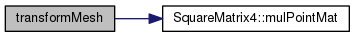
\includegraphics[width=338pt]{group__intersection__test__prperties_ga4b2a399a49c34312c8369f54b79230af_cgraph}
\end{center}
\end{figure}
\index{Intersection tests and hit object properties@{Intersection tests and hit object properties}!transform\+Plane@{transform\+Plane}}
\index{transform\+Plane@{transform\+Plane}!Intersection tests and hit object properties@{Intersection tests and hit object properties}}
\subsubsection[{\texorpdfstring{transform\+Plane(\+Dev\+Object $\ast$object, const Square\+Matrix4f \&m\+Transform)}{transformPlane(DevObject *object, const SquareMatrix4f \&mTransform)}}]{\setlength{\rightskip}{0pt plus 5cm}\+\_\+\+\_\+device\+\_\+\+\_\+ void transform\+Plane (
\begin{DoxyParamCaption}
\item[{{\bf Dev\+Object} $\ast$}]{object, }
\item[{const {\bf Square\+Matrix4f} \&}]{m\+Transform}
\end{DoxyParamCaption}
)}\hypertarget{group__intersection__test__prperties_ga6d2ae68047e8f8d11a64b9dc9dda507d}{}\label{group__intersection__test__prperties_ga6d2ae68047e8f8d11a64b9dc9dda507d}


Implicit sphere translation, rotation and scale function. 


\begin{DoxyParams}[1]{Parameters}
\mbox{\tt out}  & {\em object} & -\/ wrapper with a specific object\textquotesingle{}s data \\
\hline
\mbox{\tt in}  & {\em m\+Transform} & -\/ object-\/to-\/world matrix \\
\hline
\end{DoxyParams}
\index{Intersection tests and hit object properties@{Intersection tests and hit object properties}!transform\+Sphere@{transform\+Sphere}}
\index{transform\+Sphere@{transform\+Sphere}!Intersection tests and hit object properties@{Intersection tests and hit object properties}}
\subsubsection[{\texorpdfstring{transform\+Sphere(\+Dev\+Object $\ast$object, const Square\+Matrix4f \&m\+Transform)}{transformSphere(DevObject *object, const SquareMatrix4f \&mTransform)}}]{\setlength{\rightskip}{0pt plus 5cm}\+\_\+\+\_\+device\+\_\+\+\_\+ void transform\+Sphere (
\begin{DoxyParamCaption}
\item[{{\bf Dev\+Object} $\ast$}]{object, }
\item[{const {\bf Square\+Matrix4f} \&}]{m\+Transform}
\end{DoxyParamCaption}
)}\hypertarget{group__intersection__test__prperties_ga6fe7123c4c4bdf775eac1231bc37c490}{}\label{group__intersection__test__prperties_ga6fe7123c4c4bdf775eac1231bc37c490}


Implicit sphere translation, rotation and scale function. 


\begin{DoxyParams}[1]{Parameters}
\mbox{\tt out}  & {\em object} & -\/ wrapper with a specific object\textquotesingle{}s data \\
\hline
\mbox{\tt in}  & {\em m\+Transform} & -\/ object-\/to-\/world matrix \\
\hline
\end{DoxyParams}
Here is the call graph for this function\+:
\nopagebreak
\begin{figure}[H]
\begin{center}
\leavevmode
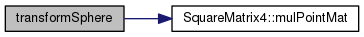
\includegraphics[width=345pt]{group__intersection__test__prperties_ga6fe7123c4c4bdf775eac1231bc37c490_cgraph}
\end{center}
\end{figure}
\index{Intersection tests and hit object properties@{Intersection tests and hit object properties}!wave@{wave}}
\index{wave@{wave}!Intersection tests and hit object properties@{Intersection tests and hit object properties}}
\subsubsection[{\texorpdfstring{wave(const Vec2f \&hit\+Tex\+Coordinates)}{wave(const Vec2f \&hitTexCoordinates)}}]{\setlength{\rightskip}{0pt plus 5cm}\+\_\+\+\_\+device\+\_\+\+\_\+ float wave (
\begin{DoxyParamCaption}
\item[{const {\bf Vec2f} \&}]{hit\+Tex\+Coordinates}
\end{DoxyParamCaption}
)}\hypertarget{group__intersection__test__prperties_gaff97add1678535636b1f4f1ca3f7a96c}{}\label{group__intersection__test__prperties_gaff97add1678535636b1f4f1ca3f7a96c}


Computes pattern at a particular point in texture. 


\begin{DoxyParams}[1]{Parameters}
\mbox{\tt in}  & {\em hit\+Tex\+Coordinates} & \\
\hline
\end{DoxyParams}
\begin{DoxyReturn}{Returns}
zero or one 
\end{DoxyReturn}

\hypertarget{group__linear__algebra}{}\section{Linear algebra}
\label{group__linear__algebra}\index{Linear algebra@{Linear algebra}}
Collaboration diagram for Linear algebra\+:
\nopagebreak
\begin{figure}[H]
\begin{center}
\leavevmode
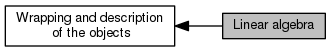
\includegraphics[width=320pt]{group__linear__algebra}
\end{center}
\end{figure}
\subsection*{Files}
\begin{DoxyCompactItemize}
\item 
file \hyperlink{r_t_tracer_2include_2geom_8cuh}{geom.\+cuh}
\item 
file \hyperlink{cuda_tracer__0__1_2include_2geom_8cuh}{geom.\+cuh}
\end{DoxyCompactItemize}
\subsection*{Classes}
\begin{DoxyCompactItemize}
\item 
class \hyperlink{class_color}{Color}
\item 
class \hyperlink{class_vec2}{Vec2}
\item 
class \hyperlink{class_vec3}{Vec3}
\item 
class \hyperlink{class_square_matrix4}{Square\+Matrix4$<$ T $>$}
\item 
class \hyperlink{class_ray}{Ray}
\item 
struct \hyperlink{struct_camera}{Camera}
\item 
class \hyperlink{class_quaternion}{Quaternion}
\item 
class \hyperlink{class_triangle}{Triangle}
\item 
struct \hyperlink{struct_vertex_properties}{Vertex\+Properties}
\begin{DoxyCompactList}\small\item\em auxiliary class for .obj files parsing. \end{DoxyCompactList}\end{DoxyCompactItemize}
\subsection*{Typedefs}
\begin{DoxyCompactItemize}
\item 
typedef \hyperlink{class_vec3}{Vec3} {\bfseries Vec3f}\hypertarget{group__linear__algebra_ga826e11f7e1e44c9038dc9cc7747b5067}{}\label{group__linear__algebra_ga826e11f7e1e44c9038dc9cc7747b5067}

\item 
typedef \hyperlink{class_vec2}{Vec2} {\bfseries Vec2f}\hypertarget{group__linear__algebra_gabe2f61ad7a1f5cdfd77e55822d77ec77}{}\label{group__linear__algebra_gabe2f61ad7a1f5cdfd77e55822d77ec77}

\item 
typedef \hyperlink{class_square_matrix4}{Square\+Matrix4}$<$ float $>$ {\bfseries Square\+Matrix4f}\hypertarget{group__linear__algebra_gad2b85d4d9fb5b5e4deaf20bff9595185}{}\label{group__linear__algebra_gad2b85d4d9fb5b5e4deaf20bff9595185}

\item 
typedef \hyperlink{class_vec3}{Vec3} {\bfseries Vec3f}\hypertarget{group__linear__algebra_ga826e11f7e1e44c9038dc9cc7747b5067}{}\label{group__linear__algebra_ga826e11f7e1e44c9038dc9cc7747b5067}

\item 
typedef \hyperlink{class_vec2}{Vec2} {\bfseries Vec2f}\hypertarget{group__linear__algebra_gabe2f61ad7a1f5cdfd77e55822d77ec77}{}\label{group__linear__algebra_gabe2f61ad7a1f5cdfd77e55822d77ec77}

\item 
typedef \hyperlink{class_square_matrix4}{Square\+Matrix4}$<$ float $>$ {\bfseries Square\+Matrix4f}\hypertarget{group__linear__algebra_gad2b85d4d9fb5b5e4deaf20bff9595185}{}\label{group__linear__algebra_gad2b85d4d9fb5b5e4deaf20bff9595185}

\end{DoxyCompactItemize}
\subsection*{Enumerations}
\begin{DoxyCompactItemize}
\item 
enum {\bfseries Ray\+Type} \{ {\bfseries P\+R\+I\+M\+A\+R\+Y\+\_\+\+R\+AY}, 
{\bfseries S\+H\+A\+D\+O\+W\+\_\+\+R\+AY}, 
{\bfseries P\+R\+I\+M\+A\+R\+Y\+\_\+\+R\+AY}, 
{\bfseries S\+H\+A\+D\+O\+W\+\_\+\+R\+AY}
 \}\hypertarget{group__linear__algebra_ga1d5111b9fffd76014406e866c8784459}{}\label{group__linear__algebra_ga1d5111b9fffd76014406e866c8784459}

\item 
enum {\bfseries Ray\+Type} \{ {\bfseries P\+R\+I\+M\+A\+R\+Y\+\_\+\+R\+AY}, 
{\bfseries S\+H\+A\+D\+O\+W\+\_\+\+R\+AY}, 
{\bfseries P\+R\+I\+M\+A\+R\+Y\+\_\+\+R\+AY}, 
{\bfseries S\+H\+A\+D\+O\+W\+\_\+\+R\+AY}
 \}\hypertarget{group__linear__algebra_ga1d5111b9fffd76014406e866c8784459}{}\label{group__linear__algebra_ga1d5111b9fffd76014406e866c8784459}

\end{DoxyCompactItemize}
\subsection*{Functions}
\begin{DoxyCompactItemize}
\item 
\+\_\+\+\_\+host\+\_\+\+\_\+ \+\_\+\+\_\+device\+\_\+\+\_\+ float {\bfseries clamp} (const float \&lo, const float \&hi, const float \&v)\hypertarget{group__linear__algebra_ga7ee7d7ce7cad4af28c138b6543fc1a81}{}\label{group__linear__algebra_ga7ee7d7ce7cad4af28c138b6543fc1a81}

\item 
constexpr double {\bfseries To\+Radian} (float x)\hypertarget{group__linear__algebra_ga542da6166501d65e2d6628718977b63f}{}\label{group__linear__algebra_ga542da6166501d65e2d6628718977b63f}

\item 
\+\_\+\+\_\+host\+\_\+\+\_\+ \+\_\+\+\_\+device\+\_\+\+\_\+ float {\bfseries deg2rad} (const float \&deg)\hypertarget{group__linear__algebra_gac2263452c984df58f61b1ef3bf96091a}{}\label{group__linear__algebra_gac2263452c984df58f61b1ef3bf96091a}

\item 
\+\_\+\+\_\+host\+\_\+\+\_\+ \+\_\+\+\_\+device\+\_\+\+\_\+ \hyperlink{class_quaternion}{Quaternion} {\bfseries operator$\ast$} (const \hyperlink{class_quaternion}{Quaternion} \&l, const \hyperlink{class_quaternion}{Quaternion} \&r)\hypertarget{group__linear__algebra_ga21d3945289653d0389e741626ab4e361}{}\label{group__linear__algebra_ga21d3945289653d0389e741626ab4e361}

\item 
\+\_\+\+\_\+host\+\_\+\+\_\+ \+\_\+\+\_\+device\+\_\+\+\_\+ \hyperlink{class_quaternion}{Quaternion} {\bfseries operator$\ast$} (const \hyperlink{class_quaternion}{Quaternion} \&q, const \hyperlink{class_vec3}{Vec3f} \&v)\hypertarget{group__linear__algebra_ga2b0200cc5ff257030068e52a4d60c5f7}{}\label{group__linear__algebra_ga2b0200cc5ff257030068e52a4d60c5f7}

\item 
\hyperlink{class_square_matrix4}{Square\+Matrix4f} {\bfseries scale} (float x, float y, float z)\hypertarget{group__linear__algebra_ga8c57bd9280eaaa89a0b823cdfd093b8f}{}\label{group__linear__algebra_ga8c57bd9280eaaa89a0b823cdfd093b8f}

\item 
\hyperlink{class_square_matrix4}{Square\+Matrix4f} {\bfseries translate} (float x, float y, float z)\hypertarget{group__linear__algebra_ga5f42c6034d55602dbab7e2306709dff0}{}\label{group__linear__algebra_ga5f42c6034d55602dbab7e2306709dff0}

\item 
\hyperlink{class_square_matrix4}{Square\+Matrix4f} \hyperlink{group__linear__algebra_gac7b995c759cd539cf455cae62c4184e6}{rotate} (const \hyperlink{class_vec3}{Vec3f} \&axis, float deg\+Angle)
\item 
\+\_\+\+\_\+host\+\_\+\+\_\+ \+\_\+\+\_\+device\+\_\+\+\_\+ \hyperlink{class_vec3}{Vec3f} \hyperlink{group__linear__algebra_ga9f88dab197e2bd7e0940faf4fd447465}{refract} (const \hyperlink{class_vec3}{Vec3f} \&incident, const \hyperlink{class_vec3}{Vec3f} \&normal, const float \&refarction\+Index)
\begin{DoxyCompactList}\small\item\em Refraction computation. \end{DoxyCompactList}\item 
\+\_\+\+\_\+host\+\_\+\+\_\+ \+\_\+\+\_\+device\+\_\+\+\_\+ void \hyperlink{group__linear__algebra_ga02c442d21d81c8d0cf889f830eddc236}{fresnel} (const \hyperlink{class_vec3}{Vec3f} \&incident, const \hyperlink{class_vec3}{Vec3f} \&normal, const float \&refraction\+Index, float \&kr)\hypertarget{group__linear__algebra_ga02c442d21d81c8d0cf889f830eddc236}{}\label{group__linear__algebra_ga02c442d21d81c8d0cf889f830eddc236}

\begin{DoxyCompactList}\small\item\em amount of reflected and refracted light computation  computes the ratio between two waves\+: parallel and perpendicular polarised light \end{DoxyCompactList}\item 
\+\_\+\+\_\+host\+\_\+\+\_\+ \+\_\+\+\_\+device\+\_\+\+\_\+ float {\bfseries height} (const \hyperlink{class_vec3}{Vec3f} \&top, const \hyperlink{class_vec3}{Vec3f} \&left, const \hyperlink{class_vec3}{Vec3f} \&right)\hypertarget{group__linear__algebra_gad27b722eda4f769baea62a2fae211b20}{}\label{group__linear__algebra_gad27b722eda4f769baea62a2fae211b20}

\item 
\+\_\+\+\_\+host\+\_\+\+\_\+ \+\_\+\+\_\+device\+\_\+\+\_\+ \hyperlink{class_vec3}{Vec3f} \hyperlink{group__linear__algebra_gac9237c364274b9a0fbb9184fae573357}{spiral} (const float \&t, const float \&R, const float \&S)
\item 
void {\bfseries set\+Color\+And\+Texture} (\hyperlink{class_vec3}{Vec3f} \&object\+Color, \hyperlink{class_vec3}{Vec3f} \&texture\+Color, std\+::string \&texturing)\hypertarget{group__linear__algebra_gad9214d8b1430de7ca564900714f22194}{}\label{group__linear__algebra_gad9214d8b1430de7ca564900714f22194}

\item 
\+\_\+\+\_\+device\+\_\+\+\_\+ \hyperlink{class_vec3}{Vec3f} \hyperlink{group__linear__algebra_ga3f0e69590f012ccde6215b3e5ccd1615}{reflect} (const \hyperlink{class_vec3}{Vec3f} \&incident, const \hyperlink{class_vec3}{Vec3f} \&normal)
\begin{DoxyCompactList}\small\item\em Reflection computation $ R = I − cos(θ)∗N − cos(θ)∗N $ (1) the formula for finding the reflection direction. \end{DoxyCompactList}\end{DoxyCompactItemize}
\subsection*{Variables}
\begin{DoxyCompactItemize}
\item 
constexpr float {\bfseries k\+Epsilon} = 1e-\/8\hypertarget{group__linear__algebra_gae5b9ba96ba9efa5b6469109acec14ce1}{}\label{group__linear__algebra_gae5b9ba96ba9efa5b6469109acec14ce1}

\item 
constexpr float {\bfseries k\+Epsilon} = 1e-\/8\hypertarget{group__linear__algebra_gae5b9ba96ba9efa5b6469109acec14ce1}{}\label{group__linear__algebra_gae5b9ba96ba9efa5b6469109acec14ce1}

\end{DoxyCompactItemize}


\subsection{Detailed Description}


\subsection{Function Documentation}
\index{Linear algebra@{Linear algebra}!reflect@{reflect}}
\index{reflect@{reflect}!Linear algebra@{Linear algebra}}
\subsubsection[{\texorpdfstring{reflect(const Vec3f \&incident, const Vec3f \&normal)}{reflect(const Vec3f \&incident, const Vec3f \&normal)}}]{\setlength{\rightskip}{0pt plus 5cm}{\bf Vec3f} reflect (
\begin{DoxyParamCaption}
\item[{const {\bf Vec3f} \&}]{incident, }
\item[{const {\bf Vec3f} \&}]{normal}
\end{DoxyParamCaption}
)}\hypertarget{group__linear__algebra_ga3f0e69590f012ccde6215b3e5ccd1615}{}\label{group__linear__algebra_ga3f0e69590f012ccde6215b3e5ccd1615}


Reflection computation $ R = I − cos(θ)∗N − cos(θ)∗N $ (1) the formula for finding the reflection direction. 

Reflection computation R = I − cos(θ)∗N − cos(θ)∗N (1) the formula for finding the reflection direction.


\begin{DoxyParams}[1]{Parameters}
\mbox{\tt in}  & {\em incident} & -\/ the directional vector of an incident ray \\
\hline
\mbox{\tt in}  & {\em normal} & -\/ a surface normal \\
\hline
\end{DoxyParams}
\index{Linear algebra@{Linear algebra}!refract@{refract}}
\index{refract@{refract}!Linear algebra@{Linear algebra}}
\subsubsection[{\texorpdfstring{refract(const Vec3f \&incident, const Vec3f \&normal, const float \&refarction\+Index)}{refract(const Vec3f \&incident, const Vec3f \&normal, const float \&refarctionIndex)}}]{\setlength{\rightskip}{0pt plus 5cm}\+\_\+\+\_\+host\+\_\+\+\_\+ \+\_\+\+\_\+device\+\_\+\+\_\+ {\bf Vec3f} refract (
\begin{DoxyParamCaption}
\item[{const {\bf Vec3f} \&}]{incident, }
\item[{const {\bf Vec3f} \&}]{normal, }
\item[{const float \&}]{refarction\+Index}
\end{DoxyParamCaption}
)}\hypertarget{group__linear__algebra_ga9f88dab197e2bd7e0940faf4fd447465}{}\label{group__linear__algebra_ga9f88dab197e2bd7e0940faf4fd447465}


Refraction computation. 

$ T=ηI+(ηc_1−c_2)N$ ,

where $η = η_1/η_2 (η$ is a refraction coefficient in the medium),

$c_1 = \cos(\theta_1) = N \cdot I,\\ $ $ c_2 = \sqrt{1 - \left( \frac{\eta_1}{\eta_2} \right) ^2 \sin^2(\theta_1)} \rightarrow \sqrt{1 - \left( \frac{\eta_1}{\eta_2} \right) ^2 (1 - \cos^2(\theta_1))}$ 
\begin{DoxyParams}[1]{Parameters}
\mbox{\tt in}  & {\em incident} & -\/ the directional vector of an incident ray \\
\hline
\mbox{\tt in}  & {\em normal} & -\/ a surface normal \\
\hline
\mbox{\tt in}  & {\em refarction\+Index} & -\/ refraction coefficient(of an object) is simply a vacuum speed of light divided by the speed of specific medium \\
\hline
\end{DoxyParams}
\index{Linear algebra@{Linear algebra}!rotate@{rotate}}
\index{rotate@{rotate}!Linear algebra@{Linear algebra}}
\subsubsection[{\texorpdfstring{rotate(const Vec3f \&axis, float deg\+Angle)}{rotate(const Vec3f \&axis, float degAngle)}}]{\setlength{\rightskip}{0pt plus 5cm}{\bf Square\+Matrix4f} rotate (
\begin{DoxyParamCaption}
\item[{const {\bf Vec3f} \&}]{axis, }
\item[{float}]{deg\+Angle}
\end{DoxyParamCaption}
)}\hypertarget{group__linear__algebra_gac7b995c759cd539cf455cae62c4184e6}{}\label{group__linear__algebra_gac7b995c759cd539cf455cae62c4184e6}
\begin{DoxyWarning}{Warning}
axis needs to be normalized 
\end{DoxyWarning}
\index{Linear algebra@{Linear algebra}!spiral@{spiral}}
\index{spiral@{spiral}!Linear algebra@{Linear algebra}}
\subsubsection[{\texorpdfstring{spiral(const float \&t, const float \&\+R, const float \&\+S)}{spiral(const float \&t, const float \&R, const float \&S)}}]{\setlength{\rightskip}{0pt plus 5cm}\+\_\+\+\_\+host\+\_\+\+\_\+ \+\_\+\+\_\+device\+\_\+\+\_\+ {\bf Vec3f} spiral (
\begin{DoxyParamCaption}
\item[{const float \&}]{t, }
\item[{const float \&}]{R, }
\item[{const float \&}]{S}
\end{DoxyParamCaption}
)}\hypertarget{group__linear__algebra_gac9237c364274b9a0fbb9184fae573357}{}\label{group__linear__algebra_gac9237c364274b9a0fbb9184fae573357}
x(t) = R $\ast$ sin(t) y(t) = R $\ast$ cos(t) z(t) = S $\ast$ t Let t -\/ parameter, R -\/ spiral radius, S -\/ скорость шага (вытянутость вдоль стержня) Here is the caller graph for this function\+:
\nopagebreak
\begin{figure}[H]
\begin{center}
\leavevmode
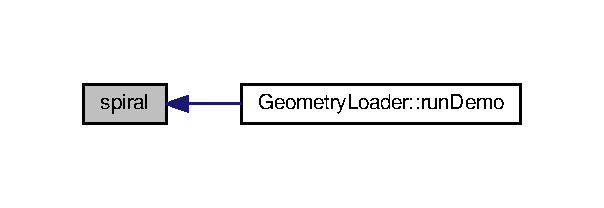
\includegraphics[width=290pt]{group__linear__algebra_gac9237c364274b9a0fbb9184fae573357_icgraph}
\end{center}
\end{figure}

\hypertarget{group__lights}{}\section{Lights}
\label{group__lights}\index{Lights@{Lights}}
Collaboration diagram for Lights\+:\nopagebreak
\begin{figure}[H]
\begin{center}
\leavevmode
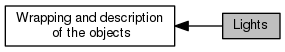
\includegraphics[width=286pt]{group__lights}
\end{center}
\end{figure}
\subsection*{Classes}
\begin{DoxyCompactItemize}
\item 
class \hyperlink{class_distant_light}{Distant\+Light$<$ Direction\+Type $>$}
\item 
class \hyperlink{class_point_light}{Point\+Light$<$ Point\+Type $>$}
\begin{DoxyCompactList}\small\item\em requires distance, unaffected by rotation \end{DoxyCompactList}\item 
class \hyperlink{class_i_light}{I\+Light}
\begin{DoxyCompactList}\small\item\em Area lights. \end{DoxyCompactList}\end{DoxyCompactItemize}
\subsection*{Typedefs}
\begin{DoxyCompactItemize}
\item 
typedef void($\ast$ {\bfseries Illuminate}) (const \hyperlink{class_i_light}{I\+Light} \&, const \hyperlink{class_vec3}{Vec3f} \&, \hyperlink{class_vec3}{Vec3f} \&, \hyperlink{class_vec3}{Vec3f} \&, float \&)\hypertarget{group__lights_ga8a5d15252b2bfd290218ef2cd88c51ee}{}\label{group__lights_ga8a5d15252b2bfd290218ef2cd88c51ee}

\item 
typedef \hyperlink{class_vec3}{Vec3f}($\ast$ {\bfseries Reflected\+Color}) (const \hyperlink{class_i_light}{I\+Light} $\ast$, \hyperlink{struct_g_p_u_1_1_rendering_context}{G\+P\+U\+::\+Rendering\+Context} \&, \hyperlink{class_vec3}{Vec3f} \&)\hypertarget{group__lights_ga1445cd39b3bf19d4237cd41d2de2243e}{}\label{group__lights_ga1445cd39b3bf19d4237cd41d2de2243e}

\end{DoxyCompactItemize}
\subsection*{Enumerations}
\begin{DoxyCompactItemize}
\item 
enum {\bfseries lights} \{ {\bfseries D\+I\+S\+T\+A\+N\+T\+\_\+\+L\+I\+G\+HT}, 
{\bfseries P\+O\+I\+N\+T\+\_\+\+L\+I\+G\+HT}
 \}\hypertarget{group__lights_ga9364632a9ecc72c4ccec5a0db539657d}{}\label{group__lights_ga9364632a9ecc72c4ccec5a0db539657d}

\end{DoxyCompactItemize}


\subsection{Detailed Description}

\hypertarget{group__usecase}{}\section{Usecase}
\label{group__usecase}\index{Usecase@{Usecase}}
Collaboration diagram for Usecase\+:\nopagebreak
\begin{figure}[H]
\begin{center}
\leavevmode
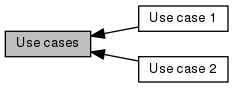
\includegraphics[width=247pt]{group__usecase}
\end{center}
\end{figure}
\subsection*{Modules}
\begin{DoxyCompactItemize}
\item 
\hyperlink{group__usecase1}{Use case 1}
\item 
\hyperlink{group__usecase2}{Use case 2}
\end{DoxyCompactItemize}


\subsection{Detailed Description}

\hypertarget{group__usecase1}{}\section{Use case 1}
\label{group__usecase1}\index{Use case 1@{Use case 1}}
Collaboration diagram for Use case 1\+:\nopagebreak
\begin{figure}[H]
\begin{center}
\leavevmode
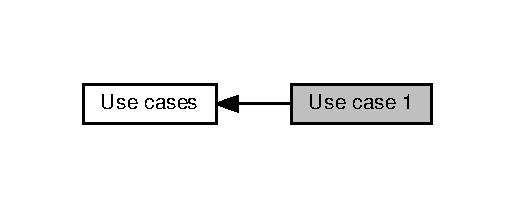
\includegraphics[width=247pt]{group__usecase1}
\end{center}
\end{figure}



\begin{DoxyCode}
\textcolor{preprocessor}{#include "bitmap.cuh"}
\textcolor{preprocessor}{#include "geometryLoader.cuh"}
\textcolor{keyword}{template} <> \textcolor{keyword}{const} \hyperlink{class_square_matrix4}{SquareMatrix4f} SquareMatrix4f::Identity = 
      \hyperlink{class_square_matrix4}{SquareMatrix4f}();
\textcolor{keywordtype}{int} main(\textcolor{keywordtype}{int} argc, \textcolor{keywordtype}{char} **argv)\{
    \hyperlink{class_vec3}{Vec3f} boundingPlaneNormals[] = \{
            \hyperlink{class_vec3}{Vec3f}(1, 0, 0),
            \hyperlink{class_vec3}{Vec3f}(0, 1, 0),
            \hyperlink{class_vec3}{Vec3f}(0, 0, 1),
            \hyperlink{class_vec3}{Vec3f}( sqrtf(3) / 3.f,  sqrtf(3) / 3.f, sqrtf(3) / 3.f),
            \hyperlink{class_vec3}{Vec3f}(-sqrtf(3) / 3.f,  sqrtf(3) / 3.f, sqrtf(3) / 3.f),
            \hyperlink{class_vec3}{Vec3f}(-sqrtf(3) / 3.f, -sqrtf(3) / 3.f, sqrtf(3) / 3.f),
            \hyperlink{class_vec3}{Vec3f}( sqrtf(3) / 3.f, -sqrtf(3) / 3.f, sqrtf(3) / 3.f) \};
        \textcolor{comment}{//Create the camera settings}
        \hyperlink{struct_camera}{Camera} camera;
        \textcolor{comment}{//set up screen width and heght, field of view and scale}
        camera.\hyperlink{struct_camera_ab0cbf1b102afdeb285ef2be271d1701c}{resolution}(960, 540, 36.87, 0.5);
        \textcolor{comment}{//create a transformation pipeline. One can set an identity matrix to not make any changes.}
        std::unique\_ptr<Pipeline> pipeline( \textcolor{keyword}{new} \hyperlink{class_mesh_transformation}{MeshTransformation}());
        pipeline->translate( make\_float3(0,0,10));
        pipeline->scale( make\_float3(1,1,1) );
        \textcolor{comment}{//Usually it's appropriate to perform the same transformation with both camera origin and camera
       direction.}
        camera.modelDir = pipeline->transform() * defaultCameraMatrix.inverse();
        camera.modelOrig = camera.modelDir;
        \textcolor{comment}{//set lights}
        std::vector<ILight> lights;
        std::unique\_ptr<Pipeline> light\_pipeline( \textcolor{keyword}{new} \hyperlink{class_mesh_transformation}{MeshTransformation}());
        \hyperlink{class_square_matrix4}{SquareMatrix4f} light\_model(0.95292, 0.289503, 0.0901785, 0,
                      -0.0960954, 0.5704, -0.815727, 0,
                      -0.287593, 0.768656, 0.571365, 0,
                    0, 0, 0, 1);
        \textcolor{comment}{//create 2 distant light sources}
        light\_pipeline->translate( make\_float3(0,0,5));
        lights.push\_back( \hyperlink{class_i_light}{ILight}( light\_model, \hyperlink{class_vec3}{Vec3f}(1, 1, 1), 1.0f, DISTANT\_LIGHT) );
        lights.push\_back( \hyperlink{class_i_light}{ILight}( light\_pipeline->transform()*light\_model, 
      \hyperlink{class_vec3}{Vec3f}(1, 1, 1), 1.0f, DISTANT\_LIGHT) );

        \textcolor{comment}{//create an instance of the specular plane settings}
        \hyperlink{struct_appearence}{Appearence} plane(0.8);
        \hyperlink{struct_appearence}{Appearence} sphere( \hyperlink{class_vec3}{Vec3f}(1,0, 0), 0.8f, 0.2f, 4.f, \textcolor{stringliteral}{"none"} );
        plane.setObjectColor(\hyperlink{class_vec3}{Vec3f}(0.5));
        plane.setTextureColor(\hyperlink{class_vec3}{Vec3f}(0.5));
        sphere.setTextureColor(\hyperlink{class_vec3}{Vec3f}(1, 0, 0 ) );
        \textcolor{comment}{// to get it into the engine one should pack it into stl vector}
        std::vector<Appearence>  appearences;
        appearences.push\_back(plane);
        appearences.push\_back(sphere);
        \textcolor{comment}{//use interface HostObject to store instances of scene geometries}
        std::vector<std::unique\_ptr<HostObject>> host\_obj;
        host\_obj.push\_back(std::unique\_ptr<HostObject>(\textcolor{keyword}{new} \hyperlink{class_plane}{Plane}( \hyperlink{class_vec3}{Vec3f}(-20, 0, 20), 
      \hyperlink{class_vec3}{Vec3f}(20, 0, 20), \hyperlink{class_vec3}{Vec3f}(20, 0, -25) )));

        host\_obj.push\_back(std::unique\_ptr<HostObject>(\textcolor{keyword}{new} \hyperlink{class_sphere}{Sphere}( \hyperlink{class_vec3}{Vec3f}(0, 10, -10), 3.0f, 
      boundingPlaneNormals )   ));
        \textcolor{comment}{//Main step. Creation of the geometry manager.}
        \hyperlink{class_geometry_loader}{GeometryLoader<Mesh, Boundaries>} loader(host\_obj, lights, 
      appearences);
        \textcolor{comment}{//Display support.}
        \hyperlink{class_bitmap_maker}{BitmapMaker< GeometryLoader<Mesh, Boundaries>} > bitmap
      (camera.width(), camera.height());
        \textcolor{keywordflow}{try}\{
            bitmap.display(camera, loader);
        \}\textcolor{keywordflow}{catch}(\textcolor{keyword}{const} std::exception& e)\{
            std::cout<<e.what()<<std::endl;
        \}

        \textcolor{keywordflow}{return} 0;
\}
\end{DoxyCode}
 
\hypertarget{group__usecase2}{}\section{Use case 2}
\label{group__usecase2}\index{Use case 2@{Use case 2}}
Collaboration diagram for Use case 2\+:\nopagebreak
\begin{figure}[H]
\begin{center}
\leavevmode
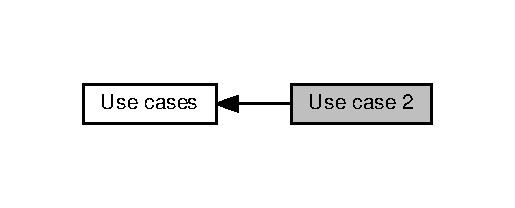
\includegraphics[width=247pt]{group__usecase2}
\end{center}
\end{figure}
Or one can use demo loader with a simple command interpreter.  
\begin{DoxyCode}
    \hyperlink{struct_camera}{Camera} camera;
camera.\hyperlink{struct_camera_ab0cbf1b102afdeb285ef2be271d1701c}{resolution}(960, 540, 36.87, 0.5);
std::unique\_ptr<Pipeline> pipeline( \textcolor{keyword}{new} \hyperlink{class_mesh_transformation}{MeshTransformation}());
pipeline->translate( make\_float3(0,0,10));
pipeline->scale( make\_float3(1,1,1) );
camera.modelDir = pipeline->transform() * defaultCameraMatrix.inverse();
camera.modelOrig = camera.modelDir;

\textcolor{comment}{//set lights}
std::vector<ILight> lights;
std::unique\_ptr<Pipeline> light\_pipeline( \textcolor{keyword}{new} \hyperlink{class_mesh_transformation}{MeshTransformation}());

\hyperlink{class_square_matrix4}{SquareMatrix4f} l2w(0.95292, 0.289503, 0.0901785, 0,
     -0.0960954, 0.5704, -0.815727, 0,
     -0.287593, 0.768656, 0.571365, 0,
         0, 0, 0, 1);
light\_pipeline->translate( make\_float3(0,0,5));
\textcolor{comment}{//lights.push\_back( ILight( l2w, Vec3f(1, 1, 1), 1.0f, DISTANT\_LIGHT) );}
lights.push\_back( \hyperlink{class_i_light}{ILight}( l2w, \hyperlink{class_vec3}{Vec3f}(1, 1, 1), 1.0f, DISTANT\_LIGHT) );
lights.push\_back( \hyperlink{class_i_light}{ILight}( light\_pipeline->transform()*l2w, \hyperlink{class_vec3}{Vec3f}(1, 1, 1), 1.0f, DISTANT\_LIGHT) 
      );
\textcolor{comment}{//Special constructor with demo launch.}
\hyperlink{class_geometry_loader}{GeometryLoader<Mesh, Boundaries>} loader(lights);
\end{DoxyCode}
 
\hypertarget{group__api__graphics}{}\section{Graphics A\+P\+Is and animation}
\label{group__api__graphics}\index{Graphics A\+P\+Is and animation@{Graphics A\+P\+Is and animation}}


Cuda-\/\+Open\+GL interoperability implementation.  


\subsection*{Classes}
\begin{DoxyCompactItemize}
\item 
class \hyperlink{class_bitmap_maker}{Bitmap\+Maker$<$ Functor $>$}
\end{DoxyCompactItemize}
\subsection*{Functions}
\begin{DoxyCompactItemize}
\item 
int {\bfseries choose\+Device} ()\hypertarget{group__api__graphics_ga17e9c55e3efd29a6c7e0705183dab8c5}{}\label{group__api__graphics_ga17e9c55e3efd29a6c7e0705183dab8c5}

\item 
{\bfseries Bitmap\+Maker$<$ Functor $>$\+::\+Bitmap\+Maker} (int width, int height)\hypertarget{group__api__graphics_ga17442bb06bac6120078e6ca3515c309f}{}\label{group__api__graphics_ga17442bb06bac6120078e6ca3515c309f}

\item 
unsigned char $\ast$ {\bfseries Bitmap\+Maker$<$ Functor $>$\+::get\+Ptr} (void) const\hypertarget{group__api__graphics_ga81b12222c93b93230e8552927deb8c77}{}\label{group__api__graphics_ga81b12222c93b93230e8552927deb8c77}

\item 
long {\bfseries Bitmap\+Maker$<$ Functor $>$\+::image\+Size} (void) const\hypertarget{group__api__graphics_gad1a201460b2575a507334385e21ac902}{}\label{group__api__graphics_gad1a201460b2575a507334385e21ac902}

\item 
unsigned char \& {\bfseries Bitmap\+Maker$<$ Functor $>$\+::operator\mbox{[}$\,$\mbox{]}} (uint32\+\_\+t i)\hypertarget{group__api__graphics_ga0bfce0b773f703313106afc3d855ac93}{}\label{group__api__graphics_ga0bfce0b773f703313106afc3d855ac93}

\item 
bool {\bfseries Bitmap\+Maker$<$ Functor $>$\+::init\+GL} ()\hypertarget{group__api__graphics_gac000f27d86706d58a359bde3b24a27f8}{}\label{group__api__graphics_gac000f27d86706d58a359bde3b24a27f8}

\item 
void {\bfseries Bitmap\+Maker$<$ Functor $>$\+::swap} (\hyperlink{class_bitmap_maker}{Bitmap\+Maker} \&bitmap)\hypertarget{group__api__graphics_ga64482b2ced38d7b7ddde58f7d9e0032b}{}\label{group__api__graphics_ga64482b2ced38d7b7ddde58f7d9e0032b}

\item 
void {\bfseries Bitmap\+Maker$<$ Functor $>$\+::create\+Buffer} (unsigned int vbo\+\_\+res\+\_\+flags)\hypertarget{group__api__graphics_gad7017ecfebf64dcc2d6881cf9c80ce39}{}\label{group__api__graphics_gad7017ecfebf64dcc2d6881cf9c80ce39}

\item 
void {\bfseries Bitmap\+Maker$<$ Functor $>$\+::delete\+Buffer} ()\hypertarget{group__api__graphics_gafdd0f7f2fa6b42b1d74158fb82d2ec04}{}\label{group__api__graphics_gafdd0f7f2fa6b42b1d74158fb82d2ec04}

\end{DoxyCompactItemize}
\subsection*{Variables}
\begin{DoxyCompactItemize}
\item 
const \hyperlink{class_square_matrix4}{Square\+Matrix4f} {\bfseries default\+Camera\+Matrix} (0.\+707107, -\/0.\+331295, 0.\+624695, 0, 0, 0.\+883452, 0.\+468521, 0, -\/0.\+707107, -\/0.\+331295, 0.\+624695, 0, -\/1.\+63871, -\/5.\+747777, -\/40.\+400412, 1)\hypertarget{group__api__graphics_gafdb8db8b7af78698e4ce48bf1ec7af05}{}\label{group__api__graphics_gafdb8db8b7af78698e4ce48bf1ec7af05}

\item 
const \hyperlink{class_square_matrix4}{Square\+Matrix4f} {\bfseries default\+Camera\+Matrix} (0.\+707107, -\/0.\+331295, 0.\+624695, 0, 0, 0.\+883452, 0.\+468521, 0, -\/0.\+707107, -\/0.\+331295, 0.\+624695, 0, -\/1.\+63871, -\/5.\+747777, -\/40.\+400412, 1)\hypertarget{group__api__graphics_gafdb8db8b7af78698e4ce48bf1ec7af05}{}\label{group__api__graphics_gafdb8db8b7af78698e4ce48bf1ec7af05}

\end{DoxyCompactItemize}


\subsection{Detailed Description}
Cuda-\/\+Open\+GL interoperability implementation. 


\hypertarget{group__device__pointers}{}\section{Device static function pointers}
\label{group__device__pointers}\index{Device static function pointers@{Device static function pointers}}
Collaboration diagram for Device static function pointers\+:\nopagebreak
\begin{figure}[H]
\begin{center}
\leavevmode
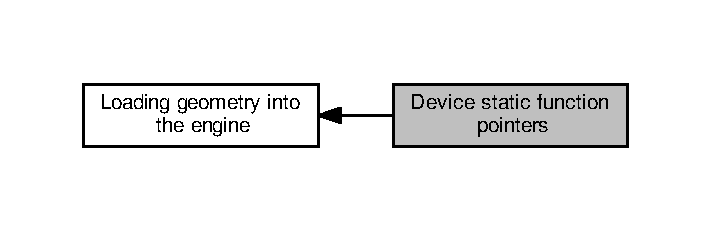
\includegraphics[width=341pt]{group__device__pointers}
\end{center}
\end{figure}
\subsection*{Typedefs}
\begin{DoxyCompactItemize}
\item 
typedef bool($\ast$ {\bfseries Intersect}) (\hyperlink{class_ray}{Ray} \&, \hyperlink{class_dev_object}{Dev\+Object} \&, \hyperlink{struct_g_p_u_1_1_rendering_context}{G\+P\+U\+::\+Rendering\+Context} \&)\hypertarget{group__device__pointers_gadd5691b4d1b8e3d72a8b279063574170}{}\label{group__device__pointers_gadd5691b4d1b8e3d72a8b279063574170}

\item 
typedef bool($\ast$ {\bfseries Intersect\+BV}) (\hyperlink{class_ray}{Ray} \&ray, float(\&precompute)\mbox{[}2\mbox{]}\mbox{[}7\mbox{]}, \hyperlink{class_dev_object}{Dev\+Object} \&current\+Object, uint8\+\_\+t \&normal\+Index)\hypertarget{group__device__pointers_ga651ba9f838240bd32d8ad85a1deec6ce}{}\label{group__device__pointers_ga651ba9f838240bd32d8ad85a1deec6ce}

\item 
typedef void($\ast$ {\bfseries Properties}) (const \hyperlink{class_dev_object}{Dev\+Object} \&object, const \hyperlink{class_vec3}{Vec3f} \&hit\+Point, \hyperlink{struct_g_p_u_1_1_rendering_context}{G\+P\+U\+::\+Rendering\+Context} \&ctx, \hyperlink{class_vec2}{Vec2f} \&hit\+Texture\+Coordinates)\hypertarget{group__device__pointers_ga3db4cb2abc6918447914228ab5019d38}{}\label{group__device__pointers_ga3db4cb2abc6918447914228ab5019d38}

\item 
typedef void($\ast$ {\bfseries Transform}) (\hyperlink{class_dev_object}{Dev\+Object} $\ast$, const \hyperlink{class_square_matrix4}{Square\+Matrix4f} \&)\hypertarget{group__device__pointers_ga7342a43dc846e3462f53f5af48daeab2}{}\label{group__device__pointers_ga7342a43dc846e3462f53f5af48daeab2}

\item 
typedef void($\ast$ {\bfseries Set\+BV}) (const \hyperlink{class_dev_object}{Dev\+Object} $\ast$, \hyperlink{class_boundaries}{Boundaries} $\ast$, \hyperlink{class_vec3}{Vec3f}(\&)\mbox{[}7\mbox{]}, float $\ast$(\&)\mbox{[}7\mbox{]})\hypertarget{group__device__pointers_gaf734749a4b67aed1bb494cb8000f870d}{}\label{group__device__pointers_gaf734749a4b67aed1bb494cb8000f870d}

\item 
typedef float($\ast$ {\bfseries Pattern}) (const \hyperlink{class_vec2}{Vec2f} \&)\hypertarget{group__device__pointers_gacb1d13948594101a67c3ec975d34e9b8}{}\label{group__device__pointers_gacb1d13948594101a67c3ec975d34e9b8}

\item 
typedef bool($\ast$ {\bfseries Intersect}) (\hyperlink{class_ray}{Ray} \&, \hyperlink{class_dev_object}{Dev\+Object} \&, \hyperlink{struct_g_p_u_1_1_rendering_context}{G\+P\+U\+::\+Rendering\+Context} \&)\hypertarget{group__device__pointers_gadd5691b4d1b8e3d72a8b279063574170}{}\label{group__device__pointers_gadd5691b4d1b8e3d72a8b279063574170}

\item 
typedef bool($\ast$ {\bfseries Intersect\+BV}) (\hyperlink{class_ray}{Ray} \&ray, float(\&precompute)\mbox{[}2\mbox{]}\mbox{[}7\mbox{]}, \hyperlink{class_dev_object}{Dev\+Object} \&current\+Object, uint8\+\_\+t \&normal\+Index)\hypertarget{group__device__pointers_ga651ba9f838240bd32d8ad85a1deec6ce}{}\label{group__device__pointers_ga651ba9f838240bd32d8ad85a1deec6ce}

\item 
typedef void($\ast$ {\bfseries Properties}) (const \hyperlink{class_dev_object}{Dev\+Object} \&object, const \hyperlink{class_vec3}{Vec3f} \&hit\+Point, \hyperlink{struct_g_p_u_1_1_rendering_context}{G\+P\+U\+::\+Rendering\+Context} \&ctx, \hyperlink{class_vec2}{Vec2f} \&hit\+Texture\+Coordinates)\hypertarget{group__device__pointers_ga3db4cb2abc6918447914228ab5019d38}{}\label{group__device__pointers_ga3db4cb2abc6918447914228ab5019d38}

\item 
typedef void($\ast$ {\bfseries Transform}) (\hyperlink{class_dev_object}{Dev\+Object} $\ast$, const \hyperlink{class_square_matrix4}{Square\+Matrix4f} \&)\hypertarget{group__device__pointers_ga7342a43dc846e3462f53f5af48daeab2}{}\label{group__device__pointers_ga7342a43dc846e3462f53f5af48daeab2}

\item 
typedef void($\ast$ {\bfseries Set\+BV}) (const \hyperlink{class_dev_object}{Dev\+Object} $\ast$, \hyperlink{class_boundaries}{Boundaries} $\ast$, \hyperlink{class_vec3}{Vec3f}(\&)\mbox{[}7\mbox{]}, float $\ast$(\&)\mbox{[}7\mbox{]})\hypertarget{group__device__pointers_gaf734749a4b67aed1bb494cb8000f870d}{}\label{group__device__pointers_gaf734749a4b67aed1bb494cb8000f870d}

\item 
typedef float($\ast$ {\bfseries Pattern}) (const \hyperlink{class_vec2}{Vec2f} \&)\hypertarget{group__device__pointers_gacb1d13948594101a67c3ec975d34e9b8}{}\label{group__device__pointers_gacb1d13948594101a67c3ec975d34e9b8}

\end{DoxyCompactItemize}
\subsection*{Variables}
\begin{DoxyCompactItemize}
\item 
\+\_\+\+\_\+device\+\_\+\+\_\+ Intersect \hyperlink{group__device__pointers_ga00654ffb007d4b5c95c00b429dc26ae9}{dev\+\_\+intersect} = \hyperlink{group__intersection__test__prperties_gac9af7cfe676f4df793dea5bc53171161}{intersect\+Mesh}\hypertarget{group__device__pointers_ga00654ffb007d4b5c95c00b429dc26ae9}{}\label{group__device__pointers_ga00654ffb007d4b5c95c00b429dc26ae9}

\begin{DoxyCompactList}\small\item\em mesh function \end{DoxyCompactList}\item 
\+\_\+\+\_\+device\+\_\+\+\_\+ Intersect\+BV \hyperlink{group__device__pointers_gaeee39cf2f67c91f2a6c312651283dc94}{dev\+\_\+intersect\+BV} = \hyperlink{group__intersection__test__prperties_gaf6bbee9e8a6ee564017fa94cd9e6ec63}{intersect\+Bounding\+Volume}\hypertarget{group__device__pointers_gaeee39cf2f67c91f2a6c312651283dc94}{}\label{group__device__pointers_gaeee39cf2f67c91f2a6c312651283dc94}

\begin{DoxyCompactList}\small\item\em mesh function \end{DoxyCompactList}\item 
\+\_\+\+\_\+device\+\_\+\+\_\+ Properties \hyperlink{group__device__pointers_gac0d627981d2453b8f45dc3cca7a69a28}{dev\+\_\+properties} = \hyperlink{group__intersection__test__prperties_gaa26e85d7aac46c25d6a1b975423f968d}{mesh\+Properties}\hypertarget{group__device__pointers_gac0d627981d2453b8f45dc3cca7a69a28}{}\label{group__device__pointers_gac0d627981d2453b8f45dc3cca7a69a28}

\begin{DoxyCompactList}\small\item\em mesh function \end{DoxyCompactList}\item 
\+\_\+\+\_\+device\+\_\+\+\_\+ Transform \hyperlink{group__device__pointers_gac3760d5ca4da6826e005200738140558}{dev\+\_\+transform} = \hyperlink{group__intersection__test__prperties_ga4b2a399a49c34312c8369f54b79230af}{transform\+Mesh}\hypertarget{group__device__pointers_gac3760d5ca4da6826e005200738140558}{}\label{group__device__pointers_gac3760d5ca4da6826e005200738140558}

\begin{DoxyCompactList}\small\item\em mesh function \end{DoxyCompactList}\item 
Set\+BV \hyperlink{group__device__pointers_gab0ffce09c75b9b50bae6f2a547e8302e}{set\+\_\+bv} = \hyperlink{group__intersection__test__prperties_ga672ecbee3aea2f5567ad7a2611feef3e}{set\+Mesh\+Acceleration\+Volume}\hypertarget{group__device__pointers_gab0ffce09c75b9b50bae6f2a547e8302e}{}\label{group__device__pointers_gab0ffce09c75b9b50bae6f2a547e8302e}

\begin{DoxyCompactList}\small\item\em mesh function \end{DoxyCompactList}\item 
\+\_\+\+\_\+device\+\_\+\+\_\+ Intersect \hyperlink{group__device__pointers_ga9e46bdfb1fa506ed7f5f6c6e11ebc091}{dev\+\_\+plane\+\_\+intersect} = \hyperlink{group__intersection__test__prperties_gafbcfd99d540347f9f63d01d6d0b6eef5}{intersect\+Plane}\hypertarget{group__device__pointers_ga9e46bdfb1fa506ed7f5f6c6e11ebc091}{}\label{group__device__pointers_ga9e46bdfb1fa506ed7f5f6c6e11ebc091}

\begin{DoxyCompactList}\small\item\em plane function \end{DoxyCompactList}\item 
\+\_\+\+\_\+device\+\_\+\+\_\+ Intersect\+BV \hyperlink{group__device__pointers_gad02954a9c76716ef59d8eda0101e15c7}{dev\+\_\+plane\+\_\+intersect\+BV} = \hyperlink{group__intersection__test__prperties_gaf6bbee9e8a6ee564017fa94cd9e6ec63}{intersect\+Bounding\+Volume}\hypertarget{group__device__pointers_gad02954a9c76716ef59d8eda0101e15c7}{}\label{group__device__pointers_gad02954a9c76716ef59d8eda0101e15c7}

\begin{DoxyCompactList}\small\item\em plane function \end{DoxyCompactList}\item 
\+\_\+\+\_\+device\+\_\+\+\_\+ Properties \hyperlink{group__device__pointers_ga31299a8a293d1f8fd1307f1e47b19b21}{dev\+\_\+plane\+\_\+properties} = \hyperlink{group__intersection__test__prperties_gae25700b3104d615db9d575d086c3d994}{plane\+Properties}\hypertarget{group__device__pointers_ga31299a8a293d1f8fd1307f1e47b19b21}{}\label{group__device__pointers_ga31299a8a293d1f8fd1307f1e47b19b21}

\begin{DoxyCompactList}\small\item\em plane function \end{DoxyCompactList}\item 
\+\_\+\+\_\+device\+\_\+\+\_\+ Transform \hyperlink{group__device__pointers_ga2515bf686c92a25ea08f35a1af5ff5af}{dev\+\_\+plane\+\_\+transform} = \hyperlink{group__intersection__test__prperties_ga6d2ae68047e8f8d11a64b9dc9dda507d}{transform\+Plane}\hypertarget{group__device__pointers_ga2515bf686c92a25ea08f35a1af5ff5af}{}\label{group__device__pointers_ga2515bf686c92a25ea08f35a1af5ff5af}

\begin{DoxyCompactList}\small\item\em plane function \end{DoxyCompactList}\item 
Set\+BV \hyperlink{group__device__pointers_gadad9e63712118e3425b0e754615f70d4}{set\+\_\+plane\+\_\+bv} = \hyperlink{group__intersection__test__prperties_ga684f41eb2add27e32a7c0115cdd6cce1}{set\+Plane\+Acceleration\+Volume}\hypertarget{group__device__pointers_gadad9e63712118e3425b0e754615f70d4}{}\label{group__device__pointers_gadad9e63712118e3425b0e754615f70d4}

\begin{DoxyCompactList}\small\item\em plane function \end{DoxyCompactList}\item 
\+\_\+\+\_\+device\+\_\+\+\_\+ Intersect \hyperlink{group__device__pointers_gafba3ff50c17e36337c7578ead7cc6f1e}{dev\+\_\+cube\+\_\+intersect} = \hyperlink{group__intersection__test__prperties_gae4778d3b0c160c9757d7fca0e5deefa2}{intersect\+Cube}\hypertarget{group__device__pointers_gafba3ff50c17e36337c7578ead7cc6f1e}{}\label{group__device__pointers_gafba3ff50c17e36337c7578ead7cc6f1e}

\begin{DoxyCompactList}\small\item\em cube function \end{DoxyCompactList}\item 
\+\_\+\+\_\+device\+\_\+\+\_\+ Intersect\+BV \hyperlink{group__device__pointers_ga0d5bc928c76877f9dd81cb8580b7fc1e}{dev\+\_\+cube\+\_\+intersect\+BV} = \hyperlink{group__intersection__test__prperties_gaf6bbee9e8a6ee564017fa94cd9e6ec63}{intersect\+Bounding\+Volume}\hypertarget{group__device__pointers_ga0d5bc928c76877f9dd81cb8580b7fc1e}{}\label{group__device__pointers_ga0d5bc928c76877f9dd81cb8580b7fc1e}

\begin{DoxyCompactList}\small\item\em cube function \end{DoxyCompactList}\item 
\+\_\+\+\_\+device\+\_\+\+\_\+ Properties \hyperlink{group__device__pointers_ga2d4562e3ca58496f57bb1d3cff526d25}{dev\+\_\+cube\+\_\+properties} = \hyperlink{group__intersection__test__prperties_ga33e6e14712999e0675085b5479201656}{cube\+Properties}\hypertarget{group__device__pointers_ga2d4562e3ca58496f57bb1d3cff526d25}{}\label{group__device__pointers_ga2d4562e3ca58496f57bb1d3cff526d25}

\begin{DoxyCompactList}\small\item\em cube function \end{DoxyCompactList}\item 
\+\_\+\+\_\+device\+\_\+\+\_\+ Transform \hyperlink{group__device__pointers_gab1b1881cdcd02a40f59daec059586d68}{dev\+\_\+cube\+\_\+transform} = \hyperlink{group__intersection__test__prperties_ga00e56ff810e7ba397e903acf50626b55}{transform\+Cube}\hypertarget{group__device__pointers_gab1b1881cdcd02a40f59daec059586d68}{}\label{group__device__pointers_gab1b1881cdcd02a40f59daec059586d68}

\begin{DoxyCompactList}\small\item\em cube function \end{DoxyCompactList}\item 
Set\+BV \hyperlink{group__device__pointers_gaec206099dfbd80a9d2e14d71b1fe150f}{set\+\_\+cube\+\_\+bv} = \hyperlink{group__intersection__test__prperties_gabfac85fdf9d0cceb70aefa4c2ed71ad2}{set\+Cube\+Acceleration\+Volume}\hypertarget{group__device__pointers_gaec206099dfbd80a9d2e14d71b1fe150f}{}\label{group__device__pointers_gaec206099dfbd80a9d2e14d71b1fe150f}

\begin{DoxyCompactList}\small\item\em cube function \end{DoxyCompactList}\item 
\+\_\+\+\_\+device\+\_\+\+\_\+ Intersect \hyperlink{group__device__pointers_ga8f39c98f1f65e4214ac0e5daa8806611}{dev\+\_\+sphere\+\_\+intersect} = \hyperlink{group__intersection__test__prperties_ga8c05ac13c3cdd49f7e4fa3948cfa4699}{intersect\+Sphere}\hypertarget{group__device__pointers_ga8f39c98f1f65e4214ac0e5daa8806611}{}\label{group__device__pointers_ga8f39c98f1f65e4214ac0e5daa8806611}

\begin{DoxyCompactList}\small\item\em sphere function \end{DoxyCompactList}\item 
\+\_\+\+\_\+device\+\_\+\+\_\+ Intersect\+BV \hyperlink{group__device__pointers_ga10dd7617749ee8f0f1766add06b56943}{dev\+\_\+sphere\+\_\+intersect\+BV} = \hyperlink{group__intersection__test__prperties_gaf6bbee9e8a6ee564017fa94cd9e6ec63}{intersect\+Bounding\+Volume}\hypertarget{group__device__pointers_ga10dd7617749ee8f0f1766add06b56943}{}\label{group__device__pointers_ga10dd7617749ee8f0f1766add06b56943}

\begin{DoxyCompactList}\small\item\em sphere function \end{DoxyCompactList}\item 
\+\_\+\+\_\+device\+\_\+\+\_\+ Properties \hyperlink{group__device__pointers_ga4d14ea4399efac27739f61e12a806591}{dev\+\_\+sphere\+\_\+properties} = \hyperlink{group__intersection__test__prperties_gae821d5671069271f7c39d22ca8950f3d}{sphere\+Properties}\hypertarget{group__device__pointers_ga4d14ea4399efac27739f61e12a806591}{}\label{group__device__pointers_ga4d14ea4399efac27739f61e12a806591}

\begin{DoxyCompactList}\small\item\em sphere function \end{DoxyCompactList}\item 
\+\_\+\+\_\+device\+\_\+\+\_\+ Transform \hyperlink{group__device__pointers_gaede5be8cca4942f24473afcbdaa177e4}{dev\+\_\+sphere\+\_\+transform} = \hyperlink{group__intersection__test__prperties_ga6fe7123c4c4bdf775eac1231bc37c490}{transform\+Sphere}\hypertarget{group__device__pointers_gaede5be8cca4942f24473afcbdaa177e4}{}\label{group__device__pointers_gaede5be8cca4942f24473afcbdaa177e4}

\begin{DoxyCompactList}\small\item\em sphere function \end{DoxyCompactList}\item 
Set\+BV \hyperlink{group__device__pointers_gac53e785e30a603faf7fd77856e39cd0f}{set\+\_\+sphere\+\_\+bv} = \hyperlink{group__intersection__test__prperties_gafd2f15ce4a55fb0d8daee0bff024b67b}{set\+Sphere\+Acceleration\+Volume}\hypertarget{group__device__pointers_gac53e785e30a603faf7fd77856e39cd0f}{}\label{group__device__pointers_gac53e785e30a603faf7fd77856e39cd0f}

\begin{DoxyCompactList}\small\item\em sphere function \end{DoxyCompactList}\item 
\+\_\+\+\_\+device\+\_\+\+\_\+ Illuminate \hyperlink{group__device__pointers_ga29d3a70fa1f9d926548b068b7cda5d44}{dev\+\_\+distant\+\_\+illuminate} = \hyperlink{group__intersection__test__prperties_ga6a438778f6ed8683785d7a892a05d312}{illuminate\+Distant}\hypertarget{group__device__pointers_ga29d3a70fa1f9d926548b068b7cda5d44}{}\label{group__device__pointers_ga29d3a70fa1f9d926548b068b7cda5d44}

\begin{DoxyCompactList}\small\item\em distant lighting function \end{DoxyCompactList}\item 
\+\_\+\+\_\+device\+\_\+\+\_\+ Illuminate \hyperlink{group__device__pointers_ga9fb3abd281c9d4d00e477db4055e3111}{dev\+\_\+point\+\_\+illuminate} = \hyperlink{group__intersection__test__prperties_gab3c663df5b5a29d04083e7793bce50d5}{illuminate\+Point}\hypertarget{group__device__pointers_ga9fb3abd281c9d4d00e477db4055e3111}{}\label{group__device__pointers_ga9fb3abd281c9d4d00e477db4055e3111}

\begin{DoxyCompactList}\small\item\em point lighting function \end{DoxyCompactList}\item 
\+\_\+\+\_\+device\+\_\+\+\_\+ Reflected\+Color \hyperlink{group__device__pointers_ga3efd041b094f1b7a7c031d9c244a0630}{dev\+\_\+distant\+\_\+reflected\+\_\+color} = \hyperlink{group__intersection__test__prperties_ga19abb6bc50199d8583aafedd0e044b7e}{distant\+Light\+Reflected\+Color}\hypertarget{group__device__pointers_ga3efd041b094f1b7a7c031d9c244a0630}{}\label{group__device__pointers_ga3efd041b094f1b7a7c031d9c244a0630}

\begin{DoxyCompactList}\small\item\em distant lighting function \end{DoxyCompactList}\item 
\+\_\+\+\_\+device\+\_\+\+\_\+ Reflected\+Color \hyperlink{group__device__pointers_ga59eceb819291c7ca1e66b767a7253dc8}{dev\+\_\+point\+\_\+reflected\+\_\+color} = \hyperlink{group__intersection__test__prperties_ga19abb6bc50199d8583aafedd0e044b7e}{distant\+Light\+Reflected\+Color}\hypertarget{group__device__pointers_ga59eceb819291c7ca1e66b767a7253dc8}{}\label{group__device__pointers_ga59eceb819291c7ca1e66b767a7253dc8}

\begin{DoxyCompactList}\small\item\em point lighting function \end{DoxyCompactList}\item 
\+\_\+\+\_\+device\+\_\+\+\_\+ Pattern \hyperlink{group__device__pointers_ga2efdb7a5e4237c7f66bf1b71f1839335}{dev\+\_\+strips} = \hyperlink{group__intersection__test__prperties_gae0b690ff7b5f9b93e53bb0c1437fbf55}{strips}\hypertarget{group__device__pointers_ga2efdb7a5e4237c7f66bf1b71f1839335}{}\label{group__device__pointers_ga2efdb7a5e4237c7f66bf1b71f1839335}

\begin{DoxyCompactList}\small\item\em texturing pattern function \end{DoxyCompactList}\item 
\+\_\+\+\_\+device\+\_\+\+\_\+ Pattern {\bfseries dev\+\_\+wave} = \hyperlink{group__intersection__test__prperties_gaff97add1678535636b1f4f1ca3f7a96c}{wave}\hypertarget{group__device__pointers_ga106fc9eb2215ecfb1360a3334a8f22dd}{}\label{group__device__pointers_ga106fc9eb2215ecfb1360a3334a8f22dd}

\item 
\+\_\+\+\_\+device\+\_\+\+\_\+ Pattern {\bfseries dev\+\_\+grid} = \hyperlink{group__intersection__test__prperties_ga4db329f1c6b211cd0ac9e6dc297f279e}{grid}\hypertarget{group__device__pointers_gaf458f0bb79e06d9beaee341c3955cb1c}{}\label{group__device__pointers_gaf458f0bb79e06d9beaee341c3955cb1c}

\item 
\+\_\+\+\_\+device\+\_\+\+\_\+ Pattern {\bfseries dev\+\_\+checker} = \hyperlink{group__intersection__test__prperties_ga100df37360dfe6954f51431bc6343dc6}{checker}\hypertarget{group__device__pointers_ga0a22f4af565cbe3e8e8eb8719d3ac30f}{}\label{group__device__pointers_ga0a22f4af565cbe3e8e8eb8719d3ac30f}

\item 
\+\_\+\+\_\+device\+\_\+\+\_\+ Pattern {\bfseries dev\+\_\+interpolation}\hypertarget{group__device__pointers_ga050793208c04dff921d09f103558fded}{}\label{group__device__pointers_ga050793208c04dff921d09f103558fded}

\item 
\+\_\+\+\_\+device\+\_\+\+\_\+ Pattern {\bfseries dev\+\_\+none} = \hyperlink{group__intersection__test__prperties_ga6ea9f9e6624268a263962a17c6634feb}{none}\hypertarget{group__device__pointers_ga5e312ec8917b7248b60bffc6f165618b}{}\label{group__device__pointers_ga5e312ec8917b7248b60bffc6f165618b}

\item 
\+\_\+\+\_\+device\+\_\+\+\_\+ Intersect \hyperlink{group__device__pointers_ga00654ffb007d4b5c95c00b429dc26ae9}{dev\+\_\+intersect} = \hyperlink{group__intersection__test__prperties_gac9af7cfe676f4df793dea5bc53171161}{intersect\+Mesh}\hypertarget{group__device__pointers_ga00654ffb007d4b5c95c00b429dc26ae9}{}\label{group__device__pointers_ga00654ffb007d4b5c95c00b429dc26ae9}

\begin{DoxyCompactList}\small\item\em mesh function \end{DoxyCompactList}\item 
\+\_\+\+\_\+device\+\_\+\+\_\+ Intersect\+BV \hyperlink{group__device__pointers_gaeee39cf2f67c91f2a6c312651283dc94}{dev\+\_\+intersect\+BV} = \hyperlink{group__intersection__test__prperties_gaf6bbee9e8a6ee564017fa94cd9e6ec63}{intersect\+Bounding\+Volume}\hypertarget{group__device__pointers_gaeee39cf2f67c91f2a6c312651283dc94}{}\label{group__device__pointers_gaeee39cf2f67c91f2a6c312651283dc94}

\begin{DoxyCompactList}\small\item\em mesh function \end{DoxyCompactList}\item 
\+\_\+\+\_\+device\+\_\+\+\_\+ Properties \hyperlink{group__device__pointers_gac0d627981d2453b8f45dc3cca7a69a28}{dev\+\_\+properties} = \hyperlink{group__intersection__test__prperties_gaa26e85d7aac46c25d6a1b975423f968d}{mesh\+Properties}\hypertarget{group__device__pointers_gac0d627981d2453b8f45dc3cca7a69a28}{}\label{group__device__pointers_gac0d627981d2453b8f45dc3cca7a69a28}

\begin{DoxyCompactList}\small\item\em mesh function \end{DoxyCompactList}\item 
\+\_\+\+\_\+device\+\_\+\+\_\+ Transform \hyperlink{group__device__pointers_gac3760d5ca4da6826e005200738140558}{dev\+\_\+transform} = \hyperlink{group__intersection__test__prperties_ga4b2a399a49c34312c8369f54b79230af}{transform\+Mesh}\hypertarget{group__device__pointers_gac3760d5ca4da6826e005200738140558}{}\label{group__device__pointers_gac3760d5ca4da6826e005200738140558}

\begin{DoxyCompactList}\small\item\em mesh function \end{DoxyCompactList}\item 
Set\+BV \hyperlink{group__device__pointers_gab0ffce09c75b9b50bae6f2a547e8302e}{set\+\_\+bv} = \hyperlink{group__intersection__test__prperties_ga672ecbee3aea2f5567ad7a2611feef3e}{set\+Mesh\+Acceleration\+Volume}\hypertarget{group__device__pointers_gab0ffce09c75b9b50bae6f2a547e8302e}{}\label{group__device__pointers_gab0ffce09c75b9b50bae6f2a547e8302e}

\begin{DoxyCompactList}\small\item\em mesh function \end{DoxyCompactList}\item 
\+\_\+\+\_\+device\+\_\+\+\_\+ Intersect \hyperlink{group__device__pointers_ga9e46bdfb1fa506ed7f5f6c6e11ebc091}{dev\+\_\+plane\+\_\+intersect} = \hyperlink{group__intersection__test__prperties_gafbcfd99d540347f9f63d01d6d0b6eef5}{intersect\+Plane}\hypertarget{group__device__pointers_ga9e46bdfb1fa506ed7f5f6c6e11ebc091}{}\label{group__device__pointers_ga9e46bdfb1fa506ed7f5f6c6e11ebc091}

\begin{DoxyCompactList}\small\item\em plane function \end{DoxyCompactList}\item 
\+\_\+\+\_\+device\+\_\+\+\_\+ Intersect\+BV \hyperlink{group__device__pointers_gad02954a9c76716ef59d8eda0101e15c7}{dev\+\_\+plane\+\_\+intersect\+BV} = \hyperlink{group__intersection__test__prperties_gaf6bbee9e8a6ee564017fa94cd9e6ec63}{intersect\+Bounding\+Volume}\hypertarget{group__device__pointers_gad02954a9c76716ef59d8eda0101e15c7}{}\label{group__device__pointers_gad02954a9c76716ef59d8eda0101e15c7}

\begin{DoxyCompactList}\small\item\em plane function \end{DoxyCompactList}\item 
\+\_\+\+\_\+device\+\_\+\+\_\+ Properties \hyperlink{group__device__pointers_ga31299a8a293d1f8fd1307f1e47b19b21}{dev\+\_\+plane\+\_\+properties} = \hyperlink{group__intersection__test__prperties_gae25700b3104d615db9d575d086c3d994}{plane\+Properties}\hypertarget{group__device__pointers_ga31299a8a293d1f8fd1307f1e47b19b21}{}\label{group__device__pointers_ga31299a8a293d1f8fd1307f1e47b19b21}

\begin{DoxyCompactList}\small\item\em plane function \end{DoxyCompactList}\item 
\+\_\+\+\_\+device\+\_\+\+\_\+ Transform \hyperlink{group__device__pointers_ga2515bf686c92a25ea08f35a1af5ff5af}{dev\+\_\+plane\+\_\+transform} = \hyperlink{group__intersection__test__prperties_ga6d2ae68047e8f8d11a64b9dc9dda507d}{transform\+Plane}\hypertarget{group__device__pointers_ga2515bf686c92a25ea08f35a1af5ff5af}{}\label{group__device__pointers_ga2515bf686c92a25ea08f35a1af5ff5af}

\begin{DoxyCompactList}\small\item\em plane function \end{DoxyCompactList}\item 
Set\+BV \hyperlink{group__device__pointers_gadad9e63712118e3425b0e754615f70d4}{set\+\_\+plane\+\_\+bv} = \hyperlink{group__intersection__test__prperties_ga684f41eb2add27e32a7c0115cdd6cce1}{set\+Plane\+Acceleration\+Volume}\hypertarget{group__device__pointers_gadad9e63712118e3425b0e754615f70d4}{}\label{group__device__pointers_gadad9e63712118e3425b0e754615f70d4}

\begin{DoxyCompactList}\small\item\em plane function \end{DoxyCompactList}\item 
\+\_\+\+\_\+device\+\_\+\+\_\+ Intersect \hyperlink{group__device__pointers_gafba3ff50c17e36337c7578ead7cc6f1e}{dev\+\_\+cube\+\_\+intersect} = \hyperlink{group__intersection__test__prperties_gae4778d3b0c160c9757d7fca0e5deefa2}{intersect\+Cube}\hypertarget{group__device__pointers_gafba3ff50c17e36337c7578ead7cc6f1e}{}\label{group__device__pointers_gafba3ff50c17e36337c7578ead7cc6f1e}

\begin{DoxyCompactList}\small\item\em cube function \end{DoxyCompactList}\item 
\+\_\+\+\_\+device\+\_\+\+\_\+ Intersect\+BV \hyperlink{group__device__pointers_ga0d5bc928c76877f9dd81cb8580b7fc1e}{dev\+\_\+cube\+\_\+intersect\+BV} = \hyperlink{group__intersection__test__prperties_gaf6bbee9e8a6ee564017fa94cd9e6ec63}{intersect\+Bounding\+Volume}\hypertarget{group__device__pointers_ga0d5bc928c76877f9dd81cb8580b7fc1e}{}\label{group__device__pointers_ga0d5bc928c76877f9dd81cb8580b7fc1e}

\begin{DoxyCompactList}\small\item\em cube function \end{DoxyCompactList}\item 
\+\_\+\+\_\+device\+\_\+\+\_\+ Properties \hyperlink{group__device__pointers_ga2d4562e3ca58496f57bb1d3cff526d25}{dev\+\_\+cube\+\_\+properties} = \hyperlink{group__intersection__test__prperties_ga33e6e14712999e0675085b5479201656}{cube\+Properties}\hypertarget{group__device__pointers_ga2d4562e3ca58496f57bb1d3cff526d25}{}\label{group__device__pointers_ga2d4562e3ca58496f57bb1d3cff526d25}

\begin{DoxyCompactList}\small\item\em cube function \end{DoxyCompactList}\item 
\+\_\+\+\_\+device\+\_\+\+\_\+ Transform \hyperlink{group__device__pointers_gab1b1881cdcd02a40f59daec059586d68}{dev\+\_\+cube\+\_\+transform} = \hyperlink{group__intersection__test__prperties_ga00e56ff810e7ba397e903acf50626b55}{transform\+Cube}\hypertarget{group__device__pointers_gab1b1881cdcd02a40f59daec059586d68}{}\label{group__device__pointers_gab1b1881cdcd02a40f59daec059586d68}

\begin{DoxyCompactList}\small\item\em cube function \end{DoxyCompactList}\item 
Set\+BV \hyperlink{group__device__pointers_gaec206099dfbd80a9d2e14d71b1fe150f}{set\+\_\+cube\+\_\+bv} = \hyperlink{group__intersection__test__prperties_gabfac85fdf9d0cceb70aefa4c2ed71ad2}{set\+Cube\+Acceleration\+Volume}\hypertarget{group__device__pointers_gaec206099dfbd80a9d2e14d71b1fe150f}{}\label{group__device__pointers_gaec206099dfbd80a9d2e14d71b1fe150f}

\begin{DoxyCompactList}\small\item\em cube function \end{DoxyCompactList}\item 
\+\_\+\+\_\+device\+\_\+\+\_\+ Intersect \hyperlink{group__device__pointers_ga8f39c98f1f65e4214ac0e5daa8806611}{dev\+\_\+sphere\+\_\+intersect} = \hyperlink{group__intersection__test__prperties_ga8c05ac13c3cdd49f7e4fa3948cfa4699}{intersect\+Sphere}\hypertarget{group__device__pointers_ga8f39c98f1f65e4214ac0e5daa8806611}{}\label{group__device__pointers_ga8f39c98f1f65e4214ac0e5daa8806611}

\begin{DoxyCompactList}\small\item\em sphere function \end{DoxyCompactList}\item 
\+\_\+\+\_\+device\+\_\+\+\_\+ Intersect\+BV \hyperlink{group__device__pointers_ga10dd7617749ee8f0f1766add06b56943}{dev\+\_\+sphere\+\_\+intersect\+BV} = \hyperlink{group__intersection__test__prperties_gaf6bbee9e8a6ee564017fa94cd9e6ec63}{intersect\+Bounding\+Volume}\hypertarget{group__device__pointers_ga10dd7617749ee8f0f1766add06b56943}{}\label{group__device__pointers_ga10dd7617749ee8f0f1766add06b56943}

\begin{DoxyCompactList}\small\item\em sphere function \end{DoxyCompactList}\item 
\+\_\+\+\_\+device\+\_\+\+\_\+ Properties \hyperlink{group__device__pointers_ga4d14ea4399efac27739f61e12a806591}{dev\+\_\+sphere\+\_\+properties} = \hyperlink{group__intersection__test__prperties_gae821d5671069271f7c39d22ca8950f3d}{sphere\+Properties}\hypertarget{group__device__pointers_ga4d14ea4399efac27739f61e12a806591}{}\label{group__device__pointers_ga4d14ea4399efac27739f61e12a806591}

\begin{DoxyCompactList}\small\item\em sphere function \end{DoxyCompactList}\item 
\+\_\+\+\_\+device\+\_\+\+\_\+ Transform \hyperlink{group__device__pointers_gaede5be8cca4942f24473afcbdaa177e4}{dev\+\_\+sphere\+\_\+transform} = \hyperlink{group__intersection__test__prperties_ga6fe7123c4c4bdf775eac1231bc37c490}{transform\+Sphere}\hypertarget{group__device__pointers_gaede5be8cca4942f24473afcbdaa177e4}{}\label{group__device__pointers_gaede5be8cca4942f24473afcbdaa177e4}

\begin{DoxyCompactList}\small\item\em sphere function \end{DoxyCompactList}\item 
Set\+BV \hyperlink{group__device__pointers_gac53e785e30a603faf7fd77856e39cd0f}{set\+\_\+sphere\+\_\+bv} = \hyperlink{group__intersection__test__prperties_gafd2f15ce4a55fb0d8daee0bff024b67b}{set\+Sphere\+Acceleration\+Volume}\hypertarget{group__device__pointers_gac53e785e30a603faf7fd77856e39cd0f}{}\label{group__device__pointers_gac53e785e30a603faf7fd77856e39cd0f}

\begin{DoxyCompactList}\small\item\em sphere function \end{DoxyCompactList}\item 
\+\_\+\+\_\+device\+\_\+\+\_\+ Illuminate \hyperlink{group__device__pointers_ga29d3a70fa1f9d926548b068b7cda5d44}{dev\+\_\+distant\+\_\+illuminate} = \hyperlink{group__intersection__test__prperties_ga6a438778f6ed8683785d7a892a05d312}{illuminate\+Distant}\hypertarget{group__device__pointers_ga29d3a70fa1f9d926548b068b7cda5d44}{}\label{group__device__pointers_ga29d3a70fa1f9d926548b068b7cda5d44}

\begin{DoxyCompactList}\small\item\em distant lighting function \end{DoxyCompactList}\item 
\+\_\+\+\_\+device\+\_\+\+\_\+ Illuminate \hyperlink{group__device__pointers_ga9fb3abd281c9d4d00e477db4055e3111}{dev\+\_\+point\+\_\+illuminate} = \hyperlink{group__intersection__test__prperties_gab3c663df5b5a29d04083e7793bce50d5}{illuminate\+Point}\hypertarget{group__device__pointers_ga9fb3abd281c9d4d00e477db4055e3111}{}\label{group__device__pointers_ga9fb3abd281c9d4d00e477db4055e3111}

\begin{DoxyCompactList}\small\item\em point lighting function \end{DoxyCompactList}\item 
\+\_\+\+\_\+device\+\_\+\+\_\+ Reflected\+Color \hyperlink{group__device__pointers_ga3efd041b094f1b7a7c031d9c244a0630}{dev\+\_\+distant\+\_\+reflected\+\_\+color} = \hyperlink{group__intersection__test__prperties_ga19abb6bc50199d8583aafedd0e044b7e}{distant\+Light\+Reflected\+Color}\hypertarget{group__device__pointers_ga3efd041b094f1b7a7c031d9c244a0630}{}\label{group__device__pointers_ga3efd041b094f1b7a7c031d9c244a0630}

\begin{DoxyCompactList}\small\item\em distant lighting function \end{DoxyCompactList}\item 
\+\_\+\+\_\+device\+\_\+\+\_\+ Reflected\+Color \hyperlink{group__device__pointers_ga59eceb819291c7ca1e66b767a7253dc8}{dev\+\_\+point\+\_\+reflected\+\_\+color} = \hyperlink{group__intersection__test__prperties_ga19abb6bc50199d8583aafedd0e044b7e}{distant\+Light\+Reflected\+Color}\hypertarget{group__device__pointers_ga59eceb819291c7ca1e66b767a7253dc8}{}\label{group__device__pointers_ga59eceb819291c7ca1e66b767a7253dc8}

\begin{DoxyCompactList}\small\item\em point lighting function \end{DoxyCompactList}\item 
\+\_\+\+\_\+device\+\_\+\+\_\+ Pattern \hyperlink{group__device__pointers_ga2efdb7a5e4237c7f66bf1b71f1839335}{dev\+\_\+strips} = \hyperlink{group__intersection__test__prperties_gae0b690ff7b5f9b93e53bb0c1437fbf55}{strips}\hypertarget{group__device__pointers_ga2efdb7a5e4237c7f66bf1b71f1839335}{}\label{group__device__pointers_ga2efdb7a5e4237c7f66bf1b71f1839335}

\begin{DoxyCompactList}\small\item\em texturing pattern function \end{DoxyCompactList}\item 
\+\_\+\+\_\+device\+\_\+\+\_\+ Pattern {\bfseries dev\+\_\+wave} = \hyperlink{group__intersection__test__prperties_gaff97add1678535636b1f4f1ca3f7a96c}{wave}\hypertarget{group__device__pointers_ga106fc9eb2215ecfb1360a3334a8f22dd}{}\label{group__device__pointers_ga106fc9eb2215ecfb1360a3334a8f22dd}

\item 
\+\_\+\+\_\+device\+\_\+\+\_\+ Pattern {\bfseries dev\+\_\+grid} = \hyperlink{group__intersection__test__prperties_ga4db329f1c6b211cd0ac9e6dc297f279e}{grid}\hypertarget{group__device__pointers_gaf458f0bb79e06d9beaee341c3955cb1c}{}\label{group__device__pointers_gaf458f0bb79e06d9beaee341c3955cb1c}

\item 
\+\_\+\+\_\+device\+\_\+\+\_\+ Pattern {\bfseries dev\+\_\+checker} = \hyperlink{group__intersection__test__prperties_ga100df37360dfe6954f51431bc6343dc6}{checker}\hypertarget{group__device__pointers_ga0a22f4af565cbe3e8e8eb8719d3ac30f}{}\label{group__device__pointers_ga0a22f4af565cbe3e8e8eb8719d3ac30f}

\item 
\+\_\+\+\_\+device\+\_\+\+\_\+ Pattern {\bfseries dev\+\_\+interpolation}\hypertarget{group__device__pointers_ga050793208c04dff921d09f103558fded}{}\label{group__device__pointers_ga050793208c04dff921d09f103558fded}

\item 
\+\_\+\+\_\+device\+\_\+\+\_\+ Pattern {\bfseries dev\+\_\+none} = \hyperlink{group__intersection__test__prperties_ga6ea9f9e6624268a263962a17c6634feb}{none}\hypertarget{group__device__pointers_ga5e312ec8917b7248b60bffc6f165618b}{}\label{group__device__pointers_ga5e312ec8917b7248b60bffc6f165618b}

\end{DoxyCompactItemize}


\subsection{Detailed Description}
-\/ The part of the polymorphic behavior implementation on both host and device sides.

-\/ Function pointer typedefs. 
\hypertarget{group__geometry__loading}{}\section{Loading geometry into the engine}
\label{group__geometry__loading}\index{Loading geometry into the engine@{Loading geometry into the engine}}


This module is designed to manage objects in both host and device memory. Currently, it maintains the triangle mesh, the light source and the implicit instances storage.  


Collaboration diagram for Loading geometry into the engine\+:
\nopagebreak
\begin{figure}[H]
\begin{center}
\leavevmode
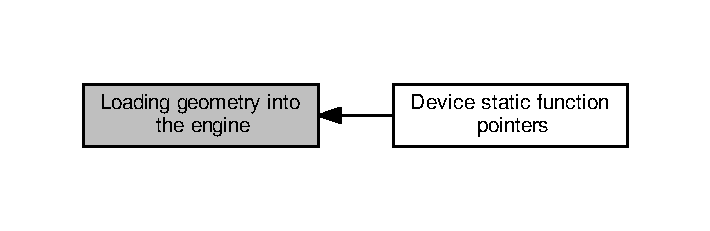
\includegraphics[width=341pt]{group__geometry__loading}
\end{center}
\end{figure}
\subsection*{Modules}
\begin{DoxyCompactItemize}
\item 
\hyperlink{group__device__pointers}{Device static function pointers}
\end{DoxyCompactItemize}
\subsection*{Classes}
\begin{DoxyCompactItemize}
\item 
class \hyperlink{class_geometry_loader}{Geometry\+Loader$<$ Objects\+Type, Bounding\+Volume\+Type $>$}
\end{DoxyCompactItemize}


\subsection{Detailed Description}
This module is designed to manage objects in both host and device memory. Currently, it maintains the triangle mesh, the light source and the implicit instances storage. 


\hypertarget{group__wrapping__and__description}{}\section{Wrapping and description of the objects}
\label{group__wrapping__and__description}\index{Wrapping and description of the objects@{Wrapping and description of the objects}}


The class stores device pointers to function That\textquotesingle{}s a part of polymorphic architecture.  


Collaboration diagram for Wrapping and description of the objects\+:
\nopagebreak
\begin{figure}[H]
\begin{center}
\leavevmode
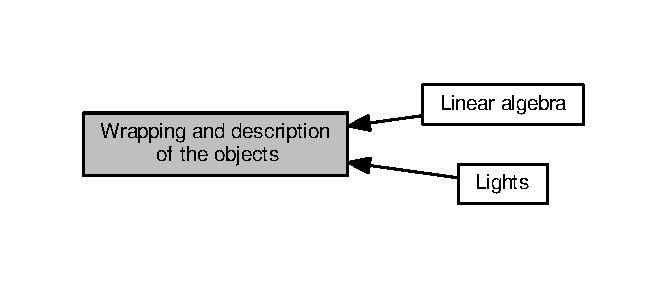
\includegraphics[width=320pt]{group__wrapping__and__description}
\end{center}
\end{figure}
\subsection*{Modules}
\begin{DoxyCompactItemize}
\item 
\hyperlink{group__linear__algebra}{Linear algebra}
\item 
\hyperlink{group__lights}{Lights}
\end{DoxyCompactItemize}
\subsection*{Classes}
\begin{DoxyCompactItemize}
\item 
struct \hyperlink{struct_polymorphic}{Polymorphic}
\item 
struct \hyperlink{struct_appearence}{Appearence}
\begin{DoxyCompactList}\small\item\em Class for textural, color and shading detail setups. \end{DoxyCompactList}\item 
class \hyperlink{class_host_object}{Host\+Object}
\begin{DoxyCompactList}\small\item\em Parent class for most of the class objects in the project except of \hyperlink{class_triangle}{Triangle} class. \end{DoxyCompactList}\item 
class \hyperlink{class_mesh}{Mesh}
\begin{DoxyCompactList}\small\item\em Class for triangulated mesh polygons. \end{DoxyCompactList}\item 
class \hyperlink{class_sphere}{Sphere}
\item 
class \hyperlink{class_plane}{Plane}
\item 
class \hyperlink{class_cube}{Cube}
\item 
class \hyperlink{class_dev_object}{Dev\+Object}
\begin{DoxyCompactList}\small\item\em Wrapper class for dynamic polymorphism on the device side. \end{DoxyCompactList}\item 
class \hyperlink{class_object_box}{Object\+Box}
\end{DoxyCompactItemize}
\subsection*{Enumerations}
\begin{DoxyCompactItemize}
\item 
enum \hyperlink{group__wrapping__and__description_ga4415a3504a4255d8563ded7496546564}{Materyal\+Type} \{ \\*
\hyperlink{group__wrapping__and__description_gga4415a3504a4255d8563ded7496546564ae24747f0d4ad269225adda5df5feaa2c}{D\+I\+F\+F\+U\+SE}, 
\hyperlink{group__wrapping__and__description_gga4415a3504a4255d8563ded7496546564abdf82a8e34e808e0be9d4765e88d6692}{R\+E\+F\+L\+E\+C\+T\+I\+ON}, 
\hyperlink{group__wrapping__and__description_gga4415a3504a4255d8563ded7496546564ab105fa30ed5e94117ebf6a37008f5e49}{P\+H\+O\+NG}, 
\hyperlink{group__wrapping__and__description_gga4415a3504a4255d8563ded7496546564ae24747f0d4ad269225adda5df5feaa2c}{D\+I\+F\+F\+U\+SE}, 
\\*
\hyperlink{group__wrapping__and__description_gga4415a3504a4255d8563ded7496546564abdf82a8e34e808e0be9d4765e88d6692}{R\+E\+F\+L\+E\+C\+T\+I\+ON}, 
\hyperlink{group__wrapping__and__description_gga4415a3504a4255d8563ded7496546564ab105fa30ed5e94117ebf6a37008f5e49}{P\+H\+O\+NG}
 \}\begin{DoxyCompactList}\small\item\em Each of the implemented shading type. \end{DoxyCompactList}
\item 
enum \hyperlink{group__wrapping__and__description_gadbd34cc71bd63d767b48ef9a2fc91c7b}{Procediral\+Texture} \{ \\*
\hyperlink{group__wrapping__and__description_ggadbd34cc71bd63d767b48ef9a2fc91c7bac157bdf0b85a40d2619cbc8bc1ae5fe2}{N\+O\+NE}, 
\hyperlink{group__wrapping__and__description_ggadbd34cc71bd63d767b48ef9a2fc91c7ba4025728e15f4cee76a85d2cc65ccb565}{W\+A\+VE}, 
\hyperlink{group__wrapping__and__description_ggadbd34cc71bd63d767b48ef9a2fc91c7ba7722877891b40e3f2d2b413d06067894}{S\+T\+R\+I\+PS}, 
\hyperlink{group__wrapping__and__description_ggadbd34cc71bd63d767b48ef9a2fc91c7bafbf4fa9eb81ba842a80a29b45064e348}{G\+R\+ID}, 
\\*
\hyperlink{group__wrapping__and__description_ggadbd34cc71bd63d767b48ef9a2fc91c7bade60519f49c1d1276c2df9c2dc500297}{C\+H\+E\+C\+K\+ER}, 
\hyperlink{group__wrapping__and__description_ggadbd34cc71bd63d767b48ef9a2fc91c7bac157bdf0b85a40d2619cbc8bc1ae5fe2}{N\+O\+NE}, 
\hyperlink{group__wrapping__and__description_ggadbd34cc71bd63d767b48ef9a2fc91c7ba4025728e15f4cee76a85d2cc65ccb565}{W\+A\+VE}, 
\hyperlink{group__wrapping__and__description_ggadbd34cc71bd63d767b48ef9a2fc91c7ba7722877891b40e3f2d2b413d06067894}{S\+T\+R\+I\+PS}, 
\\*
\hyperlink{group__wrapping__and__description_ggadbd34cc71bd63d767b48ef9a2fc91c7bafbf4fa9eb81ba842a80a29b45064e348}{G\+R\+ID}, 
\hyperlink{group__wrapping__and__description_ggadbd34cc71bd63d767b48ef9a2fc91c7bade60519f49c1d1276c2df9c2dc500297}{C\+H\+E\+C\+K\+ER}
 \}\begin{DoxyCompactList}\small\item\em Textural setup. \end{DoxyCompactList}
\item 
enum \hyperlink{group__wrapping__and__description_ga4415a3504a4255d8563ded7496546564}{Materyal\+Type} \{ \\*
\hyperlink{group__wrapping__and__description_gga4415a3504a4255d8563ded7496546564ae24747f0d4ad269225adda5df5feaa2c}{D\+I\+F\+F\+U\+SE}, 
\hyperlink{group__wrapping__and__description_gga4415a3504a4255d8563ded7496546564abdf82a8e34e808e0be9d4765e88d6692}{R\+E\+F\+L\+E\+C\+T\+I\+ON}, 
\hyperlink{group__wrapping__and__description_gga4415a3504a4255d8563ded7496546564ab105fa30ed5e94117ebf6a37008f5e49}{P\+H\+O\+NG}, 
\hyperlink{group__wrapping__and__description_gga4415a3504a4255d8563ded7496546564ae24747f0d4ad269225adda5df5feaa2c}{D\+I\+F\+F\+U\+SE}, 
\\*
\hyperlink{group__wrapping__and__description_gga4415a3504a4255d8563ded7496546564abdf82a8e34e808e0be9d4765e88d6692}{R\+E\+F\+L\+E\+C\+T\+I\+ON}, 
\hyperlink{group__wrapping__and__description_gga4415a3504a4255d8563ded7496546564ab105fa30ed5e94117ebf6a37008f5e49}{P\+H\+O\+NG}
 \}\begin{DoxyCompactList}\small\item\em Each of the implemented shading type. \end{DoxyCompactList}
\item 
enum \hyperlink{group__wrapping__and__description_gadbd34cc71bd63d767b48ef9a2fc91c7b}{Procediral\+Texture} \{ \\*
\hyperlink{group__wrapping__and__description_ggadbd34cc71bd63d767b48ef9a2fc91c7bac157bdf0b85a40d2619cbc8bc1ae5fe2}{N\+O\+NE}, 
\hyperlink{group__wrapping__and__description_ggadbd34cc71bd63d767b48ef9a2fc91c7ba4025728e15f4cee76a85d2cc65ccb565}{W\+A\+VE}, 
\hyperlink{group__wrapping__and__description_ggadbd34cc71bd63d767b48ef9a2fc91c7ba7722877891b40e3f2d2b413d06067894}{S\+T\+R\+I\+PS}, 
\hyperlink{group__wrapping__and__description_ggadbd34cc71bd63d767b48ef9a2fc91c7bafbf4fa9eb81ba842a80a29b45064e348}{G\+R\+ID}, 
\\*
\hyperlink{group__wrapping__and__description_ggadbd34cc71bd63d767b48ef9a2fc91c7bade60519f49c1d1276c2df9c2dc500297}{C\+H\+E\+C\+K\+ER}, 
\hyperlink{group__wrapping__and__description_ggadbd34cc71bd63d767b48ef9a2fc91c7bac157bdf0b85a40d2619cbc8bc1ae5fe2}{N\+O\+NE}, 
\hyperlink{group__wrapping__and__description_ggadbd34cc71bd63d767b48ef9a2fc91c7ba4025728e15f4cee76a85d2cc65ccb565}{W\+A\+VE}, 
\hyperlink{group__wrapping__and__description_ggadbd34cc71bd63d767b48ef9a2fc91c7ba7722877891b40e3f2d2b413d06067894}{S\+T\+R\+I\+PS}, 
\\*
\hyperlink{group__wrapping__and__description_ggadbd34cc71bd63d767b48ef9a2fc91c7bafbf4fa9eb81ba842a80a29b45064e348}{G\+R\+ID}, 
\hyperlink{group__wrapping__and__description_ggadbd34cc71bd63d767b48ef9a2fc91c7bade60519f49c1d1276c2df9c2dc500297}{C\+H\+E\+C\+K\+ER}
 \}\begin{DoxyCompactList}\small\item\em Textural setup. \end{DoxyCompactList}
\end{DoxyCompactItemize}


\subsection{Detailed Description}
The class stores device pointers to function That\textquotesingle{}s a part of polymorphic architecture. 



\subsection{Enumeration Type Documentation}
\index{Wrapping and description of the objects@{Wrapping and description of the objects}!Materyal\+Type@{Materyal\+Type}}
\index{Materyal\+Type@{Materyal\+Type}!Wrapping and description of the objects@{Wrapping and description of the objects}}
\subsubsection[{\texorpdfstring{Materyal\+Type}{MateryalType}}]{\setlength{\rightskip}{0pt plus 5cm}enum {\bf Materyal\+Type}}\hypertarget{group__wrapping__and__description_ga4415a3504a4255d8563ded7496546564}{}\label{group__wrapping__and__description_ga4415a3504a4255d8563ded7496546564}


Each of the implemented shading type. 

\begin{Desc}
\item[Enumerator]\par
\begin{description}
\index{D\+I\+F\+F\+U\+SE@{D\+I\+F\+F\+U\+SE}!Wrapping and description of the objects@{Wrapping and description of the objects}}\index{Wrapping and description of the objects@{Wrapping and description of the objects}!D\+I\+F\+F\+U\+SE@{D\+I\+F\+F\+U\+SE}}\item[{\em 
D\+I\+F\+F\+U\+SE\hypertarget{group__wrapping__and__description_gga4415a3504a4255d8563ded7496546564ae24747f0d4ad269225adda5df5feaa2c}{}\label{group__wrapping__and__description_gga4415a3504a4255d8563ded7496546564ae24747f0d4ad269225adda5df5feaa2c}
}]a minimum glossiness effect \index{R\+E\+F\+L\+E\+C\+T\+I\+ON@{R\+E\+F\+L\+E\+C\+T\+I\+ON}!Wrapping and description of the objects@{Wrapping and description of the objects}}\index{Wrapping and description of the objects@{Wrapping and description of the objects}!R\+E\+F\+L\+E\+C\+T\+I\+ON@{R\+E\+F\+L\+E\+C\+T\+I\+ON}}\item[{\em 
R\+E\+F\+L\+E\+C\+T\+I\+ON\hypertarget{group__wrapping__and__description_gga4415a3504a4255d8563ded7496546564abdf82a8e34e808e0be9d4765e88d6692}{}\label{group__wrapping__and__description_gga4415a3504a4255d8563ded7496546564abdf82a8e34e808e0be9d4765e88d6692}
}]a mirror surface \index{P\+H\+O\+NG@{P\+H\+O\+NG}!Wrapping and description of the objects@{Wrapping and description of the objects}}\index{Wrapping and description of the objects@{Wrapping and description of the objects}!P\+H\+O\+NG@{P\+H\+O\+NG}}\item[{\em 
P\+H\+O\+NG\hypertarget{group__wrapping__and__description_gga4415a3504a4255d8563ded7496546564ab105fa30ed5e94117ebf6a37008f5e49}{}\label{group__wrapping__and__description_gga4415a3504a4255d8563ded7496546564ab105fa30ed5e94117ebf6a37008f5e49}
}]glossiness and shininess being adjusted \index{D\+I\+F\+F\+U\+SE@{D\+I\+F\+F\+U\+SE}!Wrapping and description of the objects@{Wrapping and description of the objects}}\index{Wrapping and description of the objects@{Wrapping and description of the objects}!D\+I\+F\+F\+U\+SE@{D\+I\+F\+F\+U\+SE}}\item[{\em 
D\+I\+F\+F\+U\+SE\hypertarget{group__wrapping__and__description_gga4415a3504a4255d8563ded7496546564ae24747f0d4ad269225adda5df5feaa2c}{}\label{group__wrapping__and__description_gga4415a3504a4255d8563ded7496546564ae24747f0d4ad269225adda5df5feaa2c}
}]a minimum glossiness effect \index{R\+E\+F\+L\+E\+C\+T\+I\+ON@{R\+E\+F\+L\+E\+C\+T\+I\+ON}!Wrapping and description of the objects@{Wrapping and description of the objects}}\index{Wrapping and description of the objects@{Wrapping and description of the objects}!R\+E\+F\+L\+E\+C\+T\+I\+ON@{R\+E\+F\+L\+E\+C\+T\+I\+ON}}\item[{\em 
R\+E\+F\+L\+E\+C\+T\+I\+ON\hypertarget{group__wrapping__and__description_gga4415a3504a4255d8563ded7496546564abdf82a8e34e808e0be9d4765e88d6692}{}\label{group__wrapping__and__description_gga4415a3504a4255d8563ded7496546564abdf82a8e34e808e0be9d4765e88d6692}
}]a mirror surface \index{P\+H\+O\+NG@{P\+H\+O\+NG}!Wrapping and description of the objects@{Wrapping and description of the objects}}\index{Wrapping and description of the objects@{Wrapping and description of the objects}!P\+H\+O\+NG@{P\+H\+O\+NG}}\item[{\em 
P\+H\+O\+NG\hypertarget{group__wrapping__and__description_gga4415a3504a4255d8563ded7496546564ab105fa30ed5e94117ebf6a37008f5e49}{}\label{group__wrapping__and__description_gga4415a3504a4255d8563ded7496546564ab105fa30ed5e94117ebf6a37008f5e49}
}]glossiness and shininess being adjusted \end{description}
\end{Desc}
\index{Wrapping and description of the objects@{Wrapping and description of the objects}!Materyal\+Type@{Materyal\+Type}}
\index{Materyal\+Type@{Materyal\+Type}!Wrapping and description of the objects@{Wrapping and description of the objects}}
\subsubsection[{\texorpdfstring{Materyal\+Type}{MateryalType}}]{\setlength{\rightskip}{0pt plus 5cm}enum {\bf Materyal\+Type}}\hypertarget{group__wrapping__and__description_ga4415a3504a4255d8563ded7496546564}{}\label{group__wrapping__and__description_ga4415a3504a4255d8563ded7496546564}


Each of the implemented shading type. 

\begin{Desc}
\item[Enumerator]\par
\begin{description}
\index{D\+I\+F\+F\+U\+SE@{D\+I\+F\+F\+U\+SE}!Wrapping and description of the objects@{Wrapping and description of the objects}}\index{Wrapping and description of the objects@{Wrapping and description of the objects}!D\+I\+F\+F\+U\+SE@{D\+I\+F\+F\+U\+SE}}\item[{\em 
D\+I\+F\+F\+U\+SE\hypertarget{group__wrapping__and__description_gga4415a3504a4255d8563ded7496546564ae24747f0d4ad269225adda5df5feaa2c}{}\label{group__wrapping__and__description_gga4415a3504a4255d8563ded7496546564ae24747f0d4ad269225adda5df5feaa2c}
}]a minimum glossiness effect \index{R\+E\+F\+L\+E\+C\+T\+I\+ON@{R\+E\+F\+L\+E\+C\+T\+I\+ON}!Wrapping and description of the objects@{Wrapping and description of the objects}}\index{Wrapping and description of the objects@{Wrapping and description of the objects}!R\+E\+F\+L\+E\+C\+T\+I\+ON@{R\+E\+F\+L\+E\+C\+T\+I\+ON}}\item[{\em 
R\+E\+F\+L\+E\+C\+T\+I\+ON\hypertarget{group__wrapping__and__description_gga4415a3504a4255d8563ded7496546564abdf82a8e34e808e0be9d4765e88d6692}{}\label{group__wrapping__and__description_gga4415a3504a4255d8563ded7496546564abdf82a8e34e808e0be9d4765e88d6692}
}]a mirror surface \index{P\+H\+O\+NG@{P\+H\+O\+NG}!Wrapping and description of the objects@{Wrapping and description of the objects}}\index{Wrapping and description of the objects@{Wrapping and description of the objects}!P\+H\+O\+NG@{P\+H\+O\+NG}}\item[{\em 
P\+H\+O\+NG\hypertarget{group__wrapping__and__description_gga4415a3504a4255d8563ded7496546564ab105fa30ed5e94117ebf6a37008f5e49}{}\label{group__wrapping__and__description_gga4415a3504a4255d8563ded7496546564ab105fa30ed5e94117ebf6a37008f5e49}
}]glossiness and shininess being adjusted \index{D\+I\+F\+F\+U\+SE@{D\+I\+F\+F\+U\+SE}!Wrapping and description of the objects@{Wrapping and description of the objects}}\index{Wrapping and description of the objects@{Wrapping and description of the objects}!D\+I\+F\+F\+U\+SE@{D\+I\+F\+F\+U\+SE}}\item[{\em 
D\+I\+F\+F\+U\+SE\hypertarget{group__wrapping__and__description_gga4415a3504a4255d8563ded7496546564ae24747f0d4ad269225adda5df5feaa2c}{}\label{group__wrapping__and__description_gga4415a3504a4255d8563ded7496546564ae24747f0d4ad269225adda5df5feaa2c}
}]a minimum glossiness effect \index{R\+E\+F\+L\+E\+C\+T\+I\+ON@{R\+E\+F\+L\+E\+C\+T\+I\+ON}!Wrapping and description of the objects@{Wrapping and description of the objects}}\index{Wrapping and description of the objects@{Wrapping and description of the objects}!R\+E\+F\+L\+E\+C\+T\+I\+ON@{R\+E\+F\+L\+E\+C\+T\+I\+ON}}\item[{\em 
R\+E\+F\+L\+E\+C\+T\+I\+ON\hypertarget{group__wrapping__and__description_gga4415a3504a4255d8563ded7496546564abdf82a8e34e808e0be9d4765e88d6692}{}\label{group__wrapping__and__description_gga4415a3504a4255d8563ded7496546564abdf82a8e34e808e0be9d4765e88d6692}
}]a mirror surface \index{P\+H\+O\+NG@{P\+H\+O\+NG}!Wrapping and description of the objects@{Wrapping and description of the objects}}\index{Wrapping and description of the objects@{Wrapping and description of the objects}!P\+H\+O\+NG@{P\+H\+O\+NG}}\item[{\em 
P\+H\+O\+NG\hypertarget{group__wrapping__and__description_gga4415a3504a4255d8563ded7496546564ab105fa30ed5e94117ebf6a37008f5e49}{}\label{group__wrapping__and__description_gga4415a3504a4255d8563ded7496546564ab105fa30ed5e94117ebf6a37008f5e49}
}]glossiness and shininess being adjusted \end{description}
\end{Desc}
\index{Wrapping and description of the objects@{Wrapping and description of the objects}!Procediral\+Texture@{Procediral\+Texture}}
\index{Procediral\+Texture@{Procediral\+Texture}!Wrapping and description of the objects@{Wrapping and description of the objects}}
\subsubsection[{\texorpdfstring{Procediral\+Texture}{ProcediralTexture}}]{\setlength{\rightskip}{0pt plus 5cm}enum {\bf Procediral\+Texture}}\hypertarget{group__wrapping__and__description_gadbd34cc71bd63d767b48ef9a2fc91c7b}{}\label{group__wrapping__and__description_gadbd34cc71bd63d767b48ef9a2fc91c7b}


Textural setup. 

\begin{Desc}
\item[Enumerator]\par
\begin{description}
\index{N\+O\+NE@{N\+O\+NE}!Wrapping and description of the objects@{Wrapping and description of the objects}}\index{Wrapping and description of the objects@{Wrapping and description of the objects}!N\+O\+NE@{N\+O\+NE}}\item[{\em 
N\+O\+NE\hypertarget{group__wrapping__and__description_ggadbd34cc71bd63d767b48ef9a2fc91c7bac157bdf0b85a40d2619cbc8bc1ae5fe2}{}\label{group__wrapping__and__description_ggadbd34cc71bd63d767b48ef9a2fc91c7bac157bdf0b85a40d2619cbc8bc1ae5fe2}
}]no texture \index{W\+A\+VE@{W\+A\+VE}!Wrapping and description of the objects@{Wrapping and description of the objects}}\index{Wrapping and description of the objects@{Wrapping and description of the objects}!W\+A\+VE@{W\+A\+VE}}\item[{\em 
W\+A\+VE\hypertarget{group__wrapping__and__description_ggadbd34cc71bd63d767b48ef9a2fc91c7ba4025728e15f4cee76a85d2cc65ccb565}{}\label{group__wrapping__and__description_ggadbd34cc71bd63d767b48ef9a2fc91c7ba4025728e15f4cee76a85d2cc65ccb565}
}]blurred wave pattern \index{S\+T\+R\+I\+PS@{S\+T\+R\+I\+PS}!Wrapping and description of the objects@{Wrapping and description of the objects}}\index{Wrapping and description of the objects@{Wrapping and description of the objects}!S\+T\+R\+I\+PS@{S\+T\+R\+I\+PS}}\item[{\em 
S\+T\+R\+I\+PS\hypertarget{group__wrapping__and__description_ggadbd34cc71bd63d767b48ef9a2fc91c7ba7722877891b40e3f2d2b413d06067894}{}\label{group__wrapping__and__description_ggadbd34cc71bd63d767b48ef9a2fc91c7ba7722877891b40e3f2d2b413d06067894}
}]lines/strips pattern \index{G\+R\+ID@{G\+R\+ID}!Wrapping and description of the objects@{Wrapping and description of the objects}}\index{Wrapping and description of the objects@{Wrapping and description of the objects}!G\+R\+ID@{G\+R\+ID}}\item[{\em 
G\+R\+ID\hypertarget{group__wrapping__and__description_ggadbd34cc71bd63d767b48ef9a2fc91c7bafbf4fa9eb81ba842a80a29b45064e348}{}\label{group__wrapping__and__description_ggadbd34cc71bd63d767b48ef9a2fc91c7bafbf4fa9eb81ba842a80a29b45064e348}
}]blurred grid pattern \index{C\+H\+E\+C\+K\+ER@{C\+H\+E\+C\+K\+ER}!Wrapping and description of the objects@{Wrapping and description of the objects}}\index{Wrapping and description of the objects@{Wrapping and description of the objects}!C\+H\+E\+C\+K\+ER@{C\+H\+E\+C\+K\+ER}}\item[{\em 
C\+H\+E\+C\+K\+ER\hypertarget{group__wrapping__and__description_ggadbd34cc71bd63d767b48ef9a2fc91c7bade60519f49c1d1276c2df9c2dc500297}{}\label{group__wrapping__and__description_ggadbd34cc71bd63d767b48ef9a2fc91c7bade60519f49c1d1276c2df9c2dc500297}
}]checker pattern \index{N\+O\+NE@{N\+O\+NE}!Wrapping and description of the objects@{Wrapping and description of the objects}}\index{Wrapping and description of the objects@{Wrapping and description of the objects}!N\+O\+NE@{N\+O\+NE}}\item[{\em 
N\+O\+NE\hypertarget{group__wrapping__and__description_ggadbd34cc71bd63d767b48ef9a2fc91c7bac157bdf0b85a40d2619cbc8bc1ae5fe2}{}\label{group__wrapping__and__description_ggadbd34cc71bd63d767b48ef9a2fc91c7bac157bdf0b85a40d2619cbc8bc1ae5fe2}
}]no texture \index{W\+A\+VE@{W\+A\+VE}!Wrapping and description of the objects@{Wrapping and description of the objects}}\index{Wrapping and description of the objects@{Wrapping and description of the objects}!W\+A\+VE@{W\+A\+VE}}\item[{\em 
W\+A\+VE\hypertarget{group__wrapping__and__description_ggadbd34cc71bd63d767b48ef9a2fc91c7ba4025728e15f4cee76a85d2cc65ccb565}{}\label{group__wrapping__and__description_ggadbd34cc71bd63d767b48ef9a2fc91c7ba4025728e15f4cee76a85d2cc65ccb565}
}]blurred wave pattern \index{S\+T\+R\+I\+PS@{S\+T\+R\+I\+PS}!Wrapping and description of the objects@{Wrapping and description of the objects}}\index{Wrapping and description of the objects@{Wrapping and description of the objects}!S\+T\+R\+I\+PS@{S\+T\+R\+I\+PS}}\item[{\em 
S\+T\+R\+I\+PS\hypertarget{group__wrapping__and__description_ggadbd34cc71bd63d767b48ef9a2fc91c7ba7722877891b40e3f2d2b413d06067894}{}\label{group__wrapping__and__description_ggadbd34cc71bd63d767b48ef9a2fc91c7ba7722877891b40e3f2d2b413d06067894}
}]lines/strips pattern \index{G\+R\+ID@{G\+R\+ID}!Wrapping and description of the objects@{Wrapping and description of the objects}}\index{Wrapping and description of the objects@{Wrapping and description of the objects}!G\+R\+ID@{G\+R\+ID}}\item[{\em 
G\+R\+ID\hypertarget{group__wrapping__and__description_ggadbd34cc71bd63d767b48ef9a2fc91c7bafbf4fa9eb81ba842a80a29b45064e348}{}\label{group__wrapping__and__description_ggadbd34cc71bd63d767b48ef9a2fc91c7bafbf4fa9eb81ba842a80a29b45064e348}
}]blurred grid pattern \index{C\+H\+E\+C\+K\+ER@{C\+H\+E\+C\+K\+ER}!Wrapping and description of the objects@{Wrapping and description of the objects}}\index{Wrapping and description of the objects@{Wrapping and description of the objects}!C\+H\+E\+C\+K\+ER@{C\+H\+E\+C\+K\+ER}}\item[{\em 
C\+H\+E\+C\+K\+ER\hypertarget{group__wrapping__and__description_ggadbd34cc71bd63d767b48ef9a2fc91c7bade60519f49c1d1276c2df9c2dc500297}{}\label{group__wrapping__and__description_ggadbd34cc71bd63d767b48ef9a2fc91c7bade60519f49c1d1276c2df9c2dc500297}
}]checker pattern \end{description}
\end{Desc}
\index{Wrapping and description of the objects@{Wrapping and description of the objects}!Procediral\+Texture@{Procediral\+Texture}}
\index{Procediral\+Texture@{Procediral\+Texture}!Wrapping and description of the objects@{Wrapping and description of the objects}}
\subsubsection[{\texorpdfstring{Procediral\+Texture}{ProcediralTexture}}]{\setlength{\rightskip}{0pt plus 5cm}enum {\bf Procediral\+Texture}}\hypertarget{group__wrapping__and__description_gadbd34cc71bd63d767b48ef9a2fc91c7b}{}\label{group__wrapping__and__description_gadbd34cc71bd63d767b48ef9a2fc91c7b}


Textural setup. 

\begin{Desc}
\item[Enumerator]\par
\begin{description}
\index{N\+O\+NE@{N\+O\+NE}!Wrapping and description of the objects@{Wrapping and description of the objects}}\index{Wrapping and description of the objects@{Wrapping and description of the objects}!N\+O\+NE@{N\+O\+NE}}\item[{\em 
N\+O\+NE\hypertarget{group__wrapping__and__description_ggadbd34cc71bd63d767b48ef9a2fc91c7bac157bdf0b85a40d2619cbc8bc1ae5fe2}{}\label{group__wrapping__and__description_ggadbd34cc71bd63d767b48ef9a2fc91c7bac157bdf0b85a40d2619cbc8bc1ae5fe2}
}]no texture \index{W\+A\+VE@{W\+A\+VE}!Wrapping and description of the objects@{Wrapping and description of the objects}}\index{Wrapping and description of the objects@{Wrapping and description of the objects}!W\+A\+VE@{W\+A\+VE}}\item[{\em 
W\+A\+VE\hypertarget{group__wrapping__and__description_ggadbd34cc71bd63d767b48ef9a2fc91c7ba4025728e15f4cee76a85d2cc65ccb565}{}\label{group__wrapping__and__description_ggadbd34cc71bd63d767b48ef9a2fc91c7ba4025728e15f4cee76a85d2cc65ccb565}
}]blurred wave pattern \index{S\+T\+R\+I\+PS@{S\+T\+R\+I\+PS}!Wrapping and description of the objects@{Wrapping and description of the objects}}\index{Wrapping and description of the objects@{Wrapping and description of the objects}!S\+T\+R\+I\+PS@{S\+T\+R\+I\+PS}}\item[{\em 
S\+T\+R\+I\+PS\hypertarget{group__wrapping__and__description_ggadbd34cc71bd63d767b48ef9a2fc91c7ba7722877891b40e3f2d2b413d06067894}{}\label{group__wrapping__and__description_ggadbd34cc71bd63d767b48ef9a2fc91c7ba7722877891b40e3f2d2b413d06067894}
}]lines/strips pattern \index{G\+R\+ID@{G\+R\+ID}!Wrapping and description of the objects@{Wrapping and description of the objects}}\index{Wrapping and description of the objects@{Wrapping and description of the objects}!G\+R\+ID@{G\+R\+ID}}\item[{\em 
G\+R\+ID\hypertarget{group__wrapping__and__description_ggadbd34cc71bd63d767b48ef9a2fc91c7bafbf4fa9eb81ba842a80a29b45064e348}{}\label{group__wrapping__and__description_ggadbd34cc71bd63d767b48ef9a2fc91c7bafbf4fa9eb81ba842a80a29b45064e348}
}]blurred grid pattern \index{C\+H\+E\+C\+K\+ER@{C\+H\+E\+C\+K\+ER}!Wrapping and description of the objects@{Wrapping and description of the objects}}\index{Wrapping and description of the objects@{Wrapping and description of the objects}!C\+H\+E\+C\+K\+ER@{C\+H\+E\+C\+K\+ER}}\item[{\em 
C\+H\+E\+C\+K\+ER\hypertarget{group__wrapping__and__description_ggadbd34cc71bd63d767b48ef9a2fc91c7bade60519f49c1d1276c2df9c2dc500297}{}\label{group__wrapping__and__description_ggadbd34cc71bd63d767b48ef9a2fc91c7bade60519f49c1d1276c2df9c2dc500297}
}]checker pattern \index{N\+O\+NE@{N\+O\+NE}!Wrapping and description of the objects@{Wrapping and description of the objects}}\index{Wrapping and description of the objects@{Wrapping and description of the objects}!N\+O\+NE@{N\+O\+NE}}\item[{\em 
N\+O\+NE\hypertarget{group__wrapping__and__description_ggadbd34cc71bd63d767b48ef9a2fc91c7bac157bdf0b85a40d2619cbc8bc1ae5fe2}{}\label{group__wrapping__and__description_ggadbd34cc71bd63d767b48ef9a2fc91c7bac157bdf0b85a40d2619cbc8bc1ae5fe2}
}]no texture \index{W\+A\+VE@{W\+A\+VE}!Wrapping and description of the objects@{Wrapping and description of the objects}}\index{Wrapping and description of the objects@{Wrapping and description of the objects}!W\+A\+VE@{W\+A\+VE}}\item[{\em 
W\+A\+VE\hypertarget{group__wrapping__and__description_ggadbd34cc71bd63d767b48ef9a2fc91c7ba4025728e15f4cee76a85d2cc65ccb565}{}\label{group__wrapping__and__description_ggadbd34cc71bd63d767b48ef9a2fc91c7ba4025728e15f4cee76a85d2cc65ccb565}
}]blurred wave pattern \index{S\+T\+R\+I\+PS@{S\+T\+R\+I\+PS}!Wrapping and description of the objects@{Wrapping and description of the objects}}\index{Wrapping and description of the objects@{Wrapping and description of the objects}!S\+T\+R\+I\+PS@{S\+T\+R\+I\+PS}}\item[{\em 
S\+T\+R\+I\+PS\hypertarget{group__wrapping__and__description_ggadbd34cc71bd63d767b48ef9a2fc91c7ba7722877891b40e3f2d2b413d06067894}{}\label{group__wrapping__and__description_ggadbd34cc71bd63d767b48ef9a2fc91c7ba7722877891b40e3f2d2b413d06067894}
}]lines/strips pattern \index{G\+R\+ID@{G\+R\+ID}!Wrapping and description of the objects@{Wrapping and description of the objects}}\index{Wrapping and description of the objects@{Wrapping and description of the objects}!G\+R\+ID@{G\+R\+ID}}\item[{\em 
G\+R\+ID\hypertarget{group__wrapping__and__description_ggadbd34cc71bd63d767b48ef9a2fc91c7bafbf4fa9eb81ba842a80a29b45064e348}{}\label{group__wrapping__and__description_ggadbd34cc71bd63d767b48ef9a2fc91c7bafbf4fa9eb81ba842a80a29b45064e348}
}]blurred grid pattern \index{C\+H\+E\+C\+K\+ER@{C\+H\+E\+C\+K\+ER}!Wrapping and description of the objects@{Wrapping and description of the objects}}\index{Wrapping and description of the objects@{Wrapping and description of the objects}!C\+H\+E\+C\+K\+ER@{C\+H\+E\+C\+K\+ER}}\item[{\em 
C\+H\+E\+C\+K\+ER\hypertarget{group__wrapping__and__description_ggadbd34cc71bd63d767b48ef9a2fc91c7bade60519f49c1d1276c2df9c2dc500297}{}\label{group__wrapping__and__description_ggadbd34cc71bd63d767b48ef9a2fc91c7bade60519f49c1d1276c2df9c2dc500297}
}]checker pattern \end{description}
\end{Desc}

\hypertarget{group__rendering}{}\section{Rendering}
\label{group__rendering}\index{Rendering@{Rendering}}
Collaboration diagram for Rendering\+:\nopagebreak
\begin{figure}[H]
\begin{center}
\leavevmode
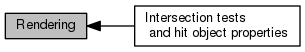
\includegraphics[width=301pt]{group__rendering}
\end{center}
\end{figure}
\subsection*{Modules}
\begin{DoxyCompactItemize}
\item 
\hyperlink{group__intersection__test__prperties}{Intersection tests and hit object properties}
\end{DoxyCompactItemize}
\subsection*{Functions}
\begin{DoxyCompactItemize}
\item 
void $\ast$ {\bfseries G\+P\+U\+::launch\+Asynch\+Ray\+Tracing} (\hyperlink{struct_camera}{Camera} cam, \hyperlink{class_object_box}{Object\+Box} \&objects, unsigned char $\ast$dev\+\_\+bitmap, dim3 \&blocks\+Per\+Grid, dim3 \&threads\+Per\+Block)\hypertarget{group__rendering_gaf46c232fe3675fb30831b3e847df0eca}{}\label{group__rendering_gaf46c232fe3675fb30831b3e847df0eca}

\item 
void \hyperlink{group__rendering_gadd1c99922e3b5c249fac22f8946b5e57}{G\+P\+U\+::render} (\hyperlink{struct_camera}{Camera} \&cam, \hyperlink{class_object_box}{Object\+Box} \&objects, unsigned char $\ast$buffer)\hypertarget{group__rendering_gadd1c99922e3b5c249fac22f8946b5e57}{}\label{group__rendering_gadd1c99922e3b5c249fac22f8946b5e57}

\begin{DoxyCompactList}\small\item\em A device kernel launcher. \end{DoxyCompactList}\item 
\+\_\+\+\_\+device\+\_\+\+\_\+ bool {\bfseries G\+P\+U\+::trace} (\hyperlink{class_ray}{Ray} \&ray, \hyperlink{class_object_box}{Object\+Box} \&objects, \hyperlink{struct_g_p_u_1_1_rendering_context}{Rendering\+Context} \&rctx, \hyperlink{class_dev_object}{Dev\+Object} $\ast$$\ast$hit\+Object, Ray\+Type raytype=P\+R\+I\+M\+A\+R\+Y\+\_\+\+R\+AY)\hypertarget{group__rendering_gab61f39aa210b4af12353c58c82b8f68e}{}\label{group__rendering_gab61f39aa210b4af12353c58c82b8f68e}

\item 
\+\_\+\+\_\+device\+\_\+\+\_\+ \hyperlink{class_vec3}{Vec3f} {\bfseries G\+P\+U\+::shade} (\hyperlink{class_ray}{Ray} \&ray, \hyperlink{class_object_box}{Object\+Box} \&obj, const \hyperlink{struct_camera}{Camera} \&options)\hypertarget{group__rendering_ga5d61799db365527e23364cea7a9f0f40}{}\label{group__rendering_ga5d61799db365527e23364cea7a9f0f40}

\item 
\+\_\+\+\_\+global\+\_\+\+\_\+ void {\bfseries raytracer} (\hyperlink{struct_camera}{Camera} cam, \hyperlink{class_object_box}{Object\+Box} objects, unsigned char $\ast$dev\+\_\+bitmap)\hypertarget{group__rendering_ga60a999f6f314338d105c33e96885a474}{}\label{group__rendering_ga60a999f6f314338d105c33e96885a474}

\end{DoxyCompactItemize}


\subsection{Detailed Description}

\chapter{Class Documentation}
\hypertarget{struct_appearence}{}\section{Appearence Struct Reference}
\label{struct_appearence}\index{Appearence@{Appearence}}


Class for textural, color and shading detail setups.  




Collaboration diagram for Appearence\+:
\nopagebreak
\begin{figure}[H]
\begin{center}
\leavevmode
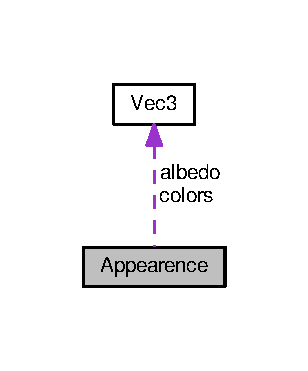
\includegraphics[width=148pt]{struct_appearence__coll__graph}
\end{center}
\end{figure}
\subsection*{Public Member Functions}
\begin{DoxyCompactItemize}
\item 
\+\_\+\+\_\+host\+\_\+\+\_\+ \+\_\+\+\_\+device\+\_\+\+\_\+ \hyperlink{struct_appearence_a0c68811b3704e25736f38c5cbb6a75bb}{Appearence} ()\hypertarget{struct_appearence_a0c68811b3704e25736f38c5cbb6a75bb}{}\label{struct_appearence_a0c68811b3704e25736f38c5cbb6a75bb}

\begin{DoxyCompactList}\small\item\em specular exponent \end{DoxyCompactList}\item 
\+\_\+\+\_\+host\+\_\+\+\_\+ \+\_\+\+\_\+device\+\_\+\+\_\+ {\bfseries Appearence} (const \hyperlink{class_vec3}{Vec3f} \&color, const float \&diffuse\+Weight, const float \&specular\+Weight, const float \&\hyperlink{struct_appearence_a6bc3ec94dc3c32295d63b09413a78252}{specular\+Exponent}, const char $\ast$texture=nullptr)\hypertarget{struct_appearence_aa99a891cc9fbedd2d11b5f927a4cce0e}{}\label{struct_appearence_aa99a891cc9fbedd2d11b5f927a4cce0e}

\item 
\+\_\+\+\_\+host\+\_\+\+\_\+ \+\_\+\+\_\+device\+\_\+\+\_\+ {\bfseries Appearence} (const \hyperlink{struct_appearence}{Appearence} \&appearence)\hypertarget{struct_appearence_a7cf2e7ec95fd1d245b4b2b22b6a2115c}{}\label{struct_appearence_a7cf2e7ec95fd1d245b4b2b22b6a2115c}

\item 
\+\_\+\+\_\+host\+\_\+\+\_\+ \+\_\+\+\_\+device\+\_\+\+\_\+ {\bfseries Appearence} (const \hyperlink{class_vec3}{Vec3f} \&color, const \hyperlink{group__wrapping__and__description_ga4415a3504a4255d8563ded7496546564}{Materyal\+Type} \&material, const float \&refraction\+Index, const float \&albedo=0.\+18f, const char $\ast$texture=nullptr, const bool \&is\+Smooth=true)\hypertarget{struct_appearence_a622c0e5e935f1a9da3bff963e2b8d6d6}{}\label{struct_appearence_a622c0e5e935f1a9da3bff963e2b8d6d6}

\item 
\+\_\+\+\_\+host\+\_\+\+\_\+ \+\_\+\+\_\+device\+\_\+\+\_\+ {\bfseries Appearence} (const \hyperlink{class_vec3}{Vec3f} \&color, const \hyperlink{group__wrapping__and__description_ga4415a3504a4255d8563ded7496546564}{Materyal\+Type} \&material)\hypertarget{struct_appearence_ad14a7f8346717aaef5c3e06d64e5d98f}{}\label{struct_appearence_ad14a7f8346717aaef5c3e06d64e5d98f}

\item 
\+\_\+\+\_\+host\+\_\+\+\_\+ \+\_\+\+\_\+device\+\_\+\+\_\+ {\bfseries Appearence} (const float \&specular\+Weight)\hypertarget{struct_appearence_a457a7a1d0c4a661efb5448d01655e537}{}\label{struct_appearence_a457a7a1d0c4a661efb5448d01655e537}

\item 
\+\_\+\+\_\+host\+\_\+\+\_\+ \+\_\+\+\_\+device\+\_\+\+\_\+ {\bfseries Appearence} (const \hyperlink{class_vec3}{Vec3f} \&color, const \hyperlink{group__wrapping__and__description_ga4415a3504a4255d8563ded7496546564}{Materyal\+Type} \&material, const float \&albedo, const char $\ast$texture=nullptr, const bool \&is\+Smooth=true)\hypertarget{struct_appearence_abcd3db2310204d26344c19cf670b81e0}{}\label{struct_appearence_abcd3db2310204d26344c19cf670b81e0}

\item 
\+\_\+\+\_\+host\+\_\+\+\_\+ \+\_\+\+\_\+device\+\_\+\+\_\+ \hyperlink{struct_appearence}{Appearence} \& {\bfseries operator=} (const \hyperlink{struct_appearence}{Appearence} \&appearence)\hypertarget{struct_appearence_ab4b59a0771673522715acf447c011a31}{}\label{struct_appearence_ab4b59a0771673522715acf447c011a31}

\item 
\+\_\+\+\_\+host\+\_\+\+\_\+ \+\_\+\+\_\+device\+\_\+\+\_\+ void {\bfseries swap} (\hyperlink{struct_appearence}{Appearence} \&appearence)\hypertarget{struct_appearence_adc2b4fb34c57083f6dfa2c7c0f649ad5}{}\label{struct_appearence_adc2b4fb34c57083f6dfa2c7c0f649ad5}

\item 
\+\_\+\+\_\+host\+\_\+\+\_\+ \+\_\+\+\_\+device\+\_\+\+\_\+ \hyperlink{struct_appearence}{Appearence} \& {\bfseries set\+Texture\+Color} (const \hyperlink{class_vec3}{Vec3f} \&color)\hypertarget{struct_appearence_af4ea9859abcc70aa41c03258b161063d}{}\label{struct_appearence_af4ea9859abcc70aa41c03258b161063d}

\item 
\+\_\+\+\_\+host\+\_\+\+\_\+ \+\_\+\+\_\+device\+\_\+\+\_\+ \hyperlink{struct_appearence}{Appearence} \& {\bfseries set\+Object\+Color} (const \hyperlink{class_vec3}{Vec3f} \&color)\hypertarget{struct_appearence_a7c0ac1007f6b1ff26fc013a2b2f1b0bc}{}\label{struct_appearence_a7c0ac1007f6b1ff26fc013a2b2f1b0bc}

\end{DoxyCompactItemize}
\subsection*{Public Attributes}
\begin{DoxyCompactItemize}
\item 
\hyperlink{group__wrapping__and__description_ga4415a3504a4255d8563ded7496546564}{Materyal\+Type} {\bfseries material}\hypertarget{struct_appearence_a1f070c81f93e329afb3c82261d0517d5}{}\label{struct_appearence_a1f070c81f93e329afb3c82261d0517d5}

\item 
float {\bfseries refraction\+Index}\hypertarget{struct_appearence_a37e85c24e1eeacd3940a79a215f99b9c}{}\label{struct_appearence_a37e85c24e1eeacd3940a79a215f99b9c}

\item 
\hyperlink{class_vec3}{Vec3f} {\bfseries albedo}\hypertarget{struct_appearence_af3f99ae57069b7b0b79c82a925eae9d3}{}\label{struct_appearence_af3f99ae57069b7b0b79c82a925eae9d3}

\item 
const char $\ast$ {\bfseries texture}\hypertarget{struct_appearence_aee82248f73c55411d26b41521f284615}{}\label{struct_appearence_aee82248f73c55411d26b41521f284615}

\item 
bool {\bfseries is\+Smooth}\hypertarget{struct_appearence_a6685d9a744c6f89bf5b52e6fba0b1b0d}{}\label{struct_appearence_a6685d9a744c6f89bf5b52e6fba0b1b0d}

\item 
\hyperlink{class_vec3}{Vec3f} \hyperlink{struct_appearence_a13dcb4d2151e8aec7e059a37a9f9ca17}{colors} \mbox{[}2\mbox{]}\hypertarget{struct_appearence_a13dcb4d2151e8aec7e059a37a9f9ca17}{}\label{struct_appearence_a13dcb4d2151e8aec7e059a37a9f9ca17}

\begin{DoxyCompactList}\small\item\em 0 is object color, 1 is texture color \end{DoxyCompactList}\item 
float {\bfseries diffuse\+Weight}\hypertarget{struct_appearence_aefd0a11e5bc797fae9676bccafa2c0d4}{}\label{struct_appearence_aefd0a11e5bc797fae9676bccafa2c0d4}

\item 
float {\bfseries specular\+Weight}\hypertarget{struct_appearence_a4baf24847b46c91c7034f96abc1591c7}{}\label{struct_appearence_a4baf24847b46c91c7034f96abc1591c7}

\item 
float \hyperlink{struct_appearence_a6bc3ec94dc3c32295d63b09413a78252}{specular\+Exponent}\hypertarget{struct_appearence_a6bc3ec94dc3c32295d63b09413a78252}{}\label{struct_appearence_a6bc3ec94dc3c32295d63b09413a78252}

\begin{DoxyCompactList}\small\item\em specular weight \end{DoxyCompactList}\end{DoxyCompactItemize}


\subsection{Detailed Description}
Class for textural, color and shading detail setups. 

The documentation for this struct was generated from the following files\+:\begin{DoxyCompactItemize}
\item 
/home/god/cuda-\/workspace/r\+T\+Tracer/include/object\+Box.\+cuh\item 
/home/god/cuda-\/workspace/r\+T\+Tracer/source/object\+Box.\+cu\end{DoxyCompactItemize}

\hypertarget{class_bitmap_maker}{}\section{Bitmap\+Maker$<$ Functor $>$ Class Template Reference}
\label{class_bitmap_maker}\index{Bitmap\+Maker$<$ Functor $>$@{Bitmap\+Maker$<$ Functor $>$}}
\subsection*{Public Member Functions}
\begin{DoxyCompactItemize}
\item 
{\bfseries Bitmap\+Maker} (int width, int height)
\item 
unsigned char $\ast$ {\bfseries get\+Ptr} (void) const
\item 
long {\bfseries image\+Size} (void) const
\item 
void {\bfseries display} (\hyperlink{struct_camera}{Camera} \&cam, Functor \&reset\+Data)\hypertarget{class_bitmap_maker_a233746936bb4d610ac0ad87094a07caf}{}\label{class_bitmap_maker_a233746936bb4d610ac0ad87094a07caf}

\item 
unsigned char \& {\bfseries operator\mbox{[}$\,$\mbox{]}} (uint32\+\_\+t i)
\item 
bool {\bfseries init\+GL} ()
\item 
void {\bfseries swap} (\hyperlink{class_bitmap_maker}{Bitmap\+Maker} \&bitmap)
\item 
void {\bfseries create\+Buffer} (unsigned int vbo\+\_\+res\+\_\+flags)
\item 
void {\bfseries delete\+Buffer} ()
\end{DoxyCompactItemize}
\subsection*{Static Public Member Functions}
\begin{DoxyCompactItemize}
\item 
static \hyperlink{class_bitmap_maker}{Bitmap\+Maker} $\ast$$\ast$ {\bfseries get\+Bitmap\+Ptr} ()\hypertarget{class_bitmap_maker_a552fe60cbd4bb0cee2abab954d3d035a}{}\label{class_bitmap_maker_a552fe60cbd4bb0cee2abab954d3d035a}

\item 
static void {\bfseries Key} (unsigned char key, int x, int y)\hypertarget{class_bitmap_maker_a5419c10622f3287678904cfe33bded58}{}\label{class_bitmap_maker_a5419c10622f3287678904cfe33bded58}

\item 
static void {\bfseries Draw} (void)\hypertarget{class_bitmap_maker_a7fbe404cf3772e9f00af0f80b8afa781}{}\label{class_bitmap_maker_a7fbe404cf3772e9f00af0f80b8afa781}

\item 
static void {\bfseries idle} ()\hypertarget{class_bitmap_maker_a0103e8746802fc4f2af3ce16a9a11613}{}\label{class_bitmap_maker_a0103e8746802fc4f2af3ce16a9a11613}

\item 
static void {\bfseries motion} (int x, int y)\hypertarget{class_bitmap_maker_af7d3a02f076e5ac261fc12ab66be9519}{}\label{class_bitmap_maker_af7d3a02f076e5ac261fc12ab66be9519}

\item 
static void {\bfseries transform\+Camera} (const std\+::unique\+\_\+ptr$<$ \hyperlink{class_pipeline}{Pipeline} $>$ \&pipeline, const \hyperlink{class_bitmap_maker}{Bitmap\+Maker} $\ast$bitmap, const \hyperlink{class_vec3}{Vec3f} \&data)\hypertarget{class_bitmap_maker_a8ea46e4e115677c1b5b52decb1e516a9}{}\label{class_bitmap_maker_a8ea46e4e115677c1b5b52decb1e516a9}

\item 
static void {\bfseries rotate\+Camera} (const std\+::unique\+\_\+ptr$<$ \hyperlink{class_pipeline}{Pipeline} $>$ \&pipeline, const \hyperlink{class_bitmap_maker}{Bitmap\+Maker} $\ast$bitmap, const \hyperlink{class_vec3}{Vec3f} \&data, const float \&delta)\hypertarget{class_bitmap_maker_a0bcc8f4a244f10901f4326ff020bb5a4}{}\label{class_bitmap_maker_a0bcc8f4a244f10901f4326ff020bb5a4}

\end{DoxyCompactItemize}
\subsection*{Public Attributes}
\begin{DoxyCompactItemize}
\item 
int {\bfseries x}\hypertarget{class_bitmap_maker_a45b158013c295196bdaa491f6acd2a5c}{}\label{class_bitmap_maker_a45b158013c295196bdaa491f6acd2a5c}

\item 
int {\bfseries y}\hypertarget{class_bitmap_maker_af790b4055fcc02c12abdc6c19563f737}{}\label{class_bitmap_maker_af790b4055fcc02c12abdc6c19563f737}

\end{DoxyCompactItemize}


The documentation for this class was generated from the following file\+:\begin{DoxyCompactItemize}
\item 
/home/god/cuda-\/workspace/r\+T\+Tracer/include/bitmap.\+cuh\end{DoxyCompactItemize}

\hypertarget{class_boundaries}{}\section{Boundaries Class Reference}
\label{class_boundaries}\index{Boundaries@{Boundaries}}
\subsection*{Public Member Functions}
\begin{DoxyCompactItemize}
\item 
\+\_\+\+\_\+host\+\_\+\+\_\+ \+\_\+\+\_\+device\+\_\+\+\_\+ bool \hyperlink{class_boundaries_ac48b60bf0de75404bb222098a890f20c}{hit} (\hyperlink{class_ray}{Ray} \&ray, float(\&precom\+Puted)\mbox{[}2\mbox{]}\mbox{[}n\+Normals\mbox{]}, uint8\+\_\+t $\ast$plane\+Index=nullptr) const
\begin{DoxyCompactList}\small\item\em hit test for a bounding volume \end{DoxyCompactList}\item 
\+\_\+\+\_\+host\+\_\+\+\_\+ \+\_\+\+\_\+device\+\_\+\+\_\+ const float \& \hyperlink{class_boundaries_a266ff06f5e1ba1f5bc69ddf8c9506186}{at} (size\+\_\+t plane\+Pair\+Number, size\+\_\+t far\+Or\+Close) const
\begin{DoxyCompactList}\small\item\em returns the distance from the origin to the bounding volume \end{DoxyCompactList}\item 
\+\_\+\+\_\+host\+\_\+\+\_\+ \+\_\+\+\_\+device\+\_\+\+\_\+ float $\ast$ \hyperlink{class_boundaries_a76d14c4bc0572159b449b47e29987690}{operator\mbox{[}$\,$\mbox{]}} (size\+\_\+t i)
\begin{DoxyCompactList}\small\item\em operator \mbox{[}\mbox{]} \end{DoxyCompactList}\end{DoxyCompactItemize}
\subsection*{Static Public Attributes}
\begin{DoxyCompactItemize}
\item 
static const uint8\+\_\+t {\bfseries n\+Normals} = N\+O\+R\+M\+A\+LS\hypertarget{class_boundaries_af0ee69c3dcc945e8e3eb5f5aa7210aae}{}\label{class_boundaries_af0ee69c3dcc945e8e3eb5f5aa7210aae}

\item 
static const uint8\+\_\+t {\bfseries n\+Plane\+Set} = N\+O\+R\+M\+A\+L\+\_\+\+S\+ET\hypertarget{class_boundaries_aee71213c990abbe66a7fbc1f694c5ebb}{}\label{class_boundaries_aee71213c990abbe66a7fbc1f694c5ebb}

\end{DoxyCompactItemize}


\subsection{Member Function Documentation}
\index{Boundaries@{Boundaries}!at@{at}}
\index{at@{at}!Boundaries@{Boundaries}}
\subsubsection[{\texorpdfstring{at(size\+\_\+t plane\+Pair\+Number, size\+\_\+t far\+Or\+Close) const}{at(size\_t planePairNumber, size\_t farOrClose) const}}]{\setlength{\rightskip}{0pt plus 5cm}\+\_\+\+\_\+host\+\_\+\+\_\+ \+\_\+\+\_\+device\+\_\+\+\_\+ const float \& Boundaries\+::at (
\begin{DoxyParamCaption}
\item[{size\+\_\+t}]{plane\+Pair\+Number, }
\item[{size\+\_\+t}]{far\+Or\+Close}
\end{DoxyParamCaption}
) const}\hypertarget{class_boundaries_a266ff06f5e1ba1f5bc69ddf8c9506186}{}\label{class_boundaries_a266ff06f5e1ba1f5bc69ddf8c9506186}


returns the distance from the origin to the bounding volume 


\begin{DoxyParams}[1]{Parameters}
\mbox{\tt in}  & {\em plane\+Pair\+Number} & -\/ a slab number to choose \\
\hline
\mbox{\tt in}  & {\em far\+Or\+Close} & -\/ choose a far or the closest bounding plane \\
\hline
\end{DoxyParams}
\begin{DoxyReturn}{Returns}
const float\& -\/ a const link to the distance from the origin to the bounding volume 
\end{DoxyReturn}
Here is the call graph for this function\+:
\nopagebreak
\begin{figure}[H]
\begin{center}
\leavevmode
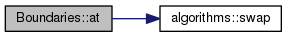
\includegraphics[width=287pt]{class_boundaries_a266ff06f5e1ba1f5bc69ddf8c9506186_cgraph}
\end{center}
\end{figure}
\index{Boundaries@{Boundaries}!hit@{hit}}
\index{hit@{hit}!Boundaries@{Boundaries}}
\subsubsection[{\texorpdfstring{hit(\+Ray \&ray, float(\&precom\+Puted)[2][n\+Normals], uint8\+\_\+t $\ast$plane\+Index=nullptr) const}{hit(Ray \&ray, float(\&precomPuted)[2][nNormals], uint8\_t *planeIndex=nullptr) const}}]{\setlength{\rightskip}{0pt plus 5cm}\+\_\+\+\_\+host\+\_\+\+\_\+ \+\_\+\+\_\+device\+\_\+\+\_\+ bool Boundaries\+::hit (
\begin{DoxyParamCaption}
\item[{{\bf Ray} \&}]{ray, }
\item[{float(\&)}]{precom\+Puted\mbox{[}2\mbox{]}\mbox{[}n\+Normals\mbox{]}, }
\item[{uint8\+\_\+t $\ast$}]{plane\+Index = {\ttfamily nullptr}}
\end{DoxyParamCaption}
) const}\hypertarget{class_boundaries_ac48b60bf0de75404bb222098a890f20c}{}\label{class_boundaries_ac48b60bf0de75404bb222098a890f20c}


hit test for a bounding volume 


\begin{DoxyParams}[1]{Parameters}
\mbox{\tt out}  & {\em ray} & -\/ sets t\+Near and t\+Far in order to determine the shortest distance on the ray \\
\hline
\mbox{\tt in}  & {\em precomputed} & -\/ numerator and denominator to accelerate the shorted hit distance \\
\hline
\mbox{\tt out}  & {\em plane\+Index} & -\/ for displaying the bounding volume. That is debug needs. \\
\hline
\end{DoxyParams}
\begin{DoxyReturn}{Returns}
bool -\/ if there was an intersection between a ray and the bounding volume 
\end{DoxyReturn}
Here is the call graph for this function\+:
\nopagebreak
\begin{figure}[H]
\begin{center}
\leavevmode
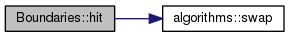
\includegraphics[width=289pt]{class_boundaries_ac48b60bf0de75404bb222098a890f20c_cgraph}
\end{center}
\end{figure}
Here is the caller graph for this function\+:
\nopagebreak
\begin{figure}[H]
\begin{center}
\leavevmode
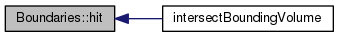
\includegraphics[width=326pt]{class_boundaries_ac48b60bf0de75404bb222098a890f20c_icgraph}
\end{center}
\end{figure}
\index{Boundaries@{Boundaries}!operator\mbox{[}$\,$\mbox{]}@{operator[]}}
\index{operator\mbox{[}$\,$\mbox{]}@{operator[]}!Boundaries@{Boundaries}}
\subsubsection[{\texorpdfstring{operator[](size\+\_\+t i)}{operator[](size\_t i)}}]{\setlength{\rightskip}{0pt plus 5cm}\+\_\+\+\_\+host\+\_\+\+\_\+ \+\_\+\+\_\+device\+\_\+\+\_\+ float$\ast$ Boundaries\+::operator\mbox{[}$\,$\mbox{]} (
\begin{DoxyParamCaption}
\item[{size\+\_\+t}]{i}
\end{DoxyParamCaption}
)\hspace{0.3cm}{\ttfamily [inline]}}\hypertarget{class_boundaries_a76d14c4bc0572159b449b47e29987690}{}\label{class_boundaries_a76d14c4bc0572159b449b47e29987690}


operator \mbox{[}\mbox{]} 


\begin{DoxyParams}[1]{Parameters}
\mbox{\tt in}  & {\em i} & -\/ choose a far or the closest bounding plane \\
\hline
\end{DoxyParams}
\begin{DoxyReturn}{Returns}
float $\ast$ -\/ a pointer to distances 
\end{DoxyReturn}


The documentation for this class was generated from the following files\+:\begin{DoxyCompactItemize}
\item 
/home/god/cuda-\/workspace/r\+T\+Tracer/include/\hyperlink{acceleration_8cuh}{acceleration.\+cuh}\item 
/home/god/cuda-\/workspace/r\+T\+Tracer/source/acceleration.\+cu\end{DoxyCompactItemize}

\hypertarget{struct_camera}{}\section{Camera Struct Reference}
\label{struct_camera}\index{Camera@{Camera}}


Collaboration diagram for Camera\+:
\nopagebreak
\begin{figure}[H]
\begin{center}
\leavevmode
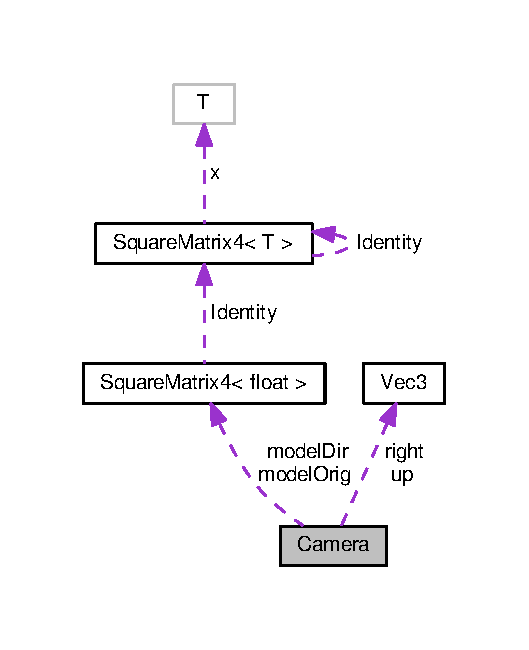
\includegraphics[width=254pt]{struct_camera__coll__graph}
\end{center}
\end{figure}
\subsection*{Public Member Functions}
\begin{DoxyCompactItemize}
\item 
void \hyperlink{struct_camera_ab0cbf1b102afdeb285ef2be271d1701c}{resolution} (size\+\_\+t \+\_\+width, size\+\_\+t \+\_\+height, const float \&\+\_\+fov, const float \&\+\_\+scale)\hypertarget{struct_camera_ab0cbf1b102afdeb285ef2be271d1701c}{}\label{struct_camera_ab0cbf1b102afdeb285ef2be271d1701c}

\begin{DoxyCompactList}\small\item\em for asyncronous kernel launch \end{DoxyCompactList}\item 
\+\_\+\+\_\+host\+\_\+\+\_\+ \+\_\+\+\_\+device\+\_\+\+\_\+ const uint \& {\bfseries width} () const\hypertarget{struct_camera_ab39e2f75274888801cca29d02f1674dd}{}\label{struct_camera_ab39e2f75274888801cca29d02f1674dd}

\item 
\+\_\+\+\_\+host\+\_\+\+\_\+ \+\_\+\+\_\+device\+\_\+\+\_\+ const uint \& {\bfseries height} () const\hypertarget{struct_camera_ab278efa15a6f64374e5d82684a75ddc4}{}\label{struct_camera_ab278efa15a6f64374e5d82684a75ddc4}

\item 
\+\_\+\+\_\+host\+\_\+\+\_\+ \+\_\+\+\_\+device\+\_\+\+\_\+ const uint \& {\bfseries partial\+Width} () const\hypertarget{struct_camera_a915024fbf05e7df1851d888395b3dad8}{}\label{struct_camera_a915024fbf05e7df1851d888395b3dad8}

\item 
\+\_\+\+\_\+host\+\_\+\+\_\+ \+\_\+\+\_\+device\+\_\+\+\_\+ const uint \& {\bfseries partial\+Height} () const\hypertarget{struct_camera_aa44087070fe5ddf954a765fef12705fa}{}\label{struct_camera_aa44087070fe5ddf954a765fef12705fa}

\item 
\+\_\+\+\_\+host\+\_\+\+\_\+ \+\_\+\+\_\+device\+\_\+\+\_\+ const float \& {\bfseries fov} () const\hypertarget{struct_camera_a048b58c104109d4a991d149ca13d28d2}{}\label{struct_camera_a048b58c104109d4a991d149ca13d28d2}

\item 
\+\_\+\+\_\+host\+\_\+\+\_\+ \+\_\+\+\_\+device\+\_\+\+\_\+ const float \& {\bfseries aspect} () const\hypertarget{struct_camera_a2a46a204df35e1f59b314cfcd7a86131}{}\label{struct_camera_a2a46a204df35e1f59b314cfcd7a86131}

\item 
\+\_\+\+\_\+host\+\_\+\+\_\+ \+\_\+\+\_\+device\+\_\+\+\_\+ const float \& {\bfseries scale} () const\hypertarget{struct_camera_a4c28d2e136f8576203213a268df461bc}{}\label{struct_camera_a4c28d2e136f8576203213a268df461bc}

\item 
void {\bfseries offset} (const int \&x, const int \&y)\hypertarget{struct_camera_ac0bcd3aa77ece7888c5bc1c894ae062a}{}\label{struct_camera_ac0bcd3aa77ece7888c5bc1c894ae062a}

\item 
\+\_\+\+\_\+host\+\_\+\+\_\+ \+\_\+\+\_\+device\+\_\+\+\_\+ const int \& {\bfseries x\+Offset} () const\hypertarget{struct_camera_a4d4292bd655023cc379de72e600aa135}{}\label{struct_camera_a4d4292bd655023cc379de72e600aa135}

\item 
\+\_\+\+\_\+host\+\_\+\+\_\+ \+\_\+\+\_\+device\+\_\+\+\_\+ const int \& {\bfseries y\+Offset} () const\hypertarget{struct_camera_af87e905be8647ef1e492f56fe35b243d}{}\label{struct_camera_af87e905be8647ef1e492f56fe35b243d}

\item 
void \hyperlink{struct_camera_ab0cbf1b102afdeb285ef2be271d1701c}{resolution} (size\+\_\+t \+\_\+width, size\+\_\+t \+\_\+height, const float \&\+\_\+fov, const float \&\+\_\+scale)\hypertarget{struct_camera_ab0cbf1b102afdeb285ef2be271d1701c}{}\label{struct_camera_ab0cbf1b102afdeb285ef2be271d1701c}

\begin{DoxyCompactList}\small\item\em for asyncronous kernel launch \end{DoxyCompactList}\item 
\+\_\+\+\_\+host\+\_\+\+\_\+ \+\_\+\+\_\+device\+\_\+\+\_\+ const uint \& {\bfseries width} () const\hypertarget{struct_camera_a558884ad2cb0294e590e92dbfa8c2cd6}{}\label{struct_camera_a558884ad2cb0294e590e92dbfa8c2cd6}

\item 
\+\_\+\+\_\+host\+\_\+\+\_\+ \+\_\+\+\_\+device\+\_\+\+\_\+ const uint \& {\bfseries height} () const\hypertarget{struct_camera_a57d4b05077eb80513ecad514982237ba}{}\label{struct_camera_a57d4b05077eb80513ecad514982237ba}

\item 
\+\_\+\+\_\+host\+\_\+\+\_\+ \+\_\+\+\_\+device\+\_\+\+\_\+ const uint \& {\bfseries partial\+Width} () const\hypertarget{struct_camera_acd260957ed8b8a4eeb9508518208bc0d}{}\label{struct_camera_acd260957ed8b8a4eeb9508518208bc0d}

\item 
\+\_\+\+\_\+host\+\_\+\+\_\+ \+\_\+\+\_\+device\+\_\+\+\_\+ const uint \& {\bfseries partial\+Height} () const\hypertarget{struct_camera_ab2c6118ca30fc99ec534d191c074279c}{}\label{struct_camera_ab2c6118ca30fc99ec534d191c074279c}

\item 
\+\_\+\+\_\+host\+\_\+\+\_\+ \+\_\+\+\_\+device\+\_\+\+\_\+ const float \& {\bfseries fov} () const\hypertarget{struct_camera_a3b18014eda80437e57d5293a846bca40}{}\label{struct_camera_a3b18014eda80437e57d5293a846bca40}

\item 
\+\_\+\+\_\+host\+\_\+\+\_\+ \+\_\+\+\_\+device\+\_\+\+\_\+ const float \& {\bfseries aspect} () const\hypertarget{struct_camera_ab6076c70d19aa5839112a033511e2640}{}\label{struct_camera_ab6076c70d19aa5839112a033511e2640}

\item 
\+\_\+\+\_\+host\+\_\+\+\_\+ \+\_\+\+\_\+device\+\_\+\+\_\+ const float \& {\bfseries scale} () const\hypertarget{struct_camera_a73cfa71841467a185998ea264839b111}{}\label{struct_camera_a73cfa71841467a185998ea264839b111}

\item 
void {\bfseries offset} (const int \&x, const int \&y)\hypertarget{struct_camera_ac0bcd3aa77ece7888c5bc1c894ae062a}{}\label{struct_camera_ac0bcd3aa77ece7888c5bc1c894ae062a}

\item 
\+\_\+\+\_\+host\+\_\+\+\_\+ \+\_\+\+\_\+device\+\_\+\+\_\+ const int \& {\bfseries x\+Offset} () const\hypertarget{struct_camera_a34b7f842855e92f9458b1e09a2952b9d}{}\label{struct_camera_a34b7f842855e92f9458b1e09a2952b9d}

\item 
\+\_\+\+\_\+host\+\_\+\+\_\+ \+\_\+\+\_\+device\+\_\+\+\_\+ const int \& {\bfseries y\+Offset} () const\hypertarget{struct_camera_a232d7fb3ef648735930cebebaa1510fe}{}\label{struct_camera_a232d7fb3ef648735930cebebaa1510fe}

\end{DoxyCompactItemize}
\subsection*{Public Attributes}
\begin{DoxyCompactItemize}
\item 
\hyperlink{class_square_matrix4}{Square\+Matrix4f} {\bfseries model\+Dir}\hypertarget{struct_camera_aca61ca4fe4b4822de05bdc0881648dc5}{}\label{struct_camera_aca61ca4fe4b4822de05bdc0881648dc5}

\item 
\hyperlink{class_square_matrix4}{Square\+Matrix4f} {\bfseries model\+Orig}\hypertarget{struct_camera_ad8d667d7e8292ddef386fee085f981dd}{}\label{struct_camera_ad8d667d7e8292ddef386fee085f981dd}

\item 
bool {\bfseries on\+Keyboard} = false\hypertarget{struct_camera_ad0c8d1b86ab1589f62827e69336265c9}{}\label{struct_camera_ad0c8d1b86ab1589f62827e69336265c9}

\item 
bool \hyperlink{struct_camera_ac8c147911753dc1cf3a7a2b8219011c4}{on\+Mouse} = false\hypertarget{struct_camera_ac8c147911753dc1cf3a7a2b8219011c4}{}\label{struct_camera_ac8c147911753dc1cf3a7a2b8219011c4}

\begin{DoxyCompactList}\small\item\em if key is pressed \end{DoxyCompactList}\item 
\hyperlink{class_vec3}{Vec3f} {\bfseries up} = \hyperlink{class_vec3}{Vec3f}(0, 1, 0)\hypertarget{struct_camera_ace6326d21c5f4e8aad4314a99839bafd}{}\label{struct_camera_ace6326d21c5f4e8aad4314a99839bafd}

\item 
\hyperlink{class_vec3}{Vec3f} {\bfseries right} = \hyperlink{class_vec3}{Vec3f}(1, 0, 0)\hypertarget{struct_camera_a382a2d324a00da22f61d5694e3ba535e}{}\label{struct_camera_a382a2d324a00da22f61d5694e3ba535e}

\end{DoxyCompactItemize}


\subsection{Detailed Description}
A camera class. Rays are transmitted through the origin along the direction. The position of the camera is stored in model matrix. 

The documentation for this struct was generated from the following files\+:\begin{DoxyCompactItemize}
\item 
/home/god/cuda-\/workspace/r\+T\+Tracer/include/\hyperlink{r_t_tracer_2include_2geom_8cuh}{geom.\+cuh}\item 
/home/god/cuda-\/workspace/r\+T\+Tracer/source/geom.\+cu\end{DoxyCompactItemize}

\hypertarget{class_color}{}\section{Color Class Reference}
\label{class_color}\index{Color@{Color}}
\subsection*{Public Member Functions}
\begin{DoxyCompactItemize}
\item 
\+\_\+\+\_\+host\+\_\+\+\_\+ \+\_\+\+\_\+device\+\_\+\+\_\+ {\bfseries Color} (float red, float green, float blue)\hypertarget{class_color_a6a7cb8dac1635db291832221f50e6342}{}\label{class_color_a6a7cb8dac1635db291832221f50e6342}

\item 
\+\_\+\+\_\+host\+\_\+\+\_\+ \+\_\+\+\_\+device\+\_\+\+\_\+ \hyperlink{class_color}{Color} {\bfseries operator$\ast$} (const float \&pattern) const\hypertarget{class_color_a81ac566b8402177923ba530c7eefd8da}{}\label{class_color_a81ac566b8402177923ba530c7eefd8da}

\end{DoxyCompactItemize}
\subsection*{Public Attributes}
\begin{DoxyCompactItemize}
\item 
float {\bfseries r}\hypertarget{class_color_a3958a556b47d2de3dd45c75aac833c20}{}\label{class_color_a3958a556b47d2de3dd45c75aac833c20}

\item 
float {\bfseries g}\hypertarget{class_color_a5defbb21620e480e556181772d665f34}{}\label{class_color_a5defbb21620e480e556181772d665f34}

\item 
float {\bfseries b}\hypertarget{class_color_a33e482be18d6ea31d2b403bee13683b7}{}\label{class_color_a33e482be18d6ea31d2b403bee13683b7}

\end{DoxyCompactItemize}


The documentation for this class was generated from the following files\+:\begin{DoxyCompactItemize}
\item 
/home/god/cuda-\/workspace/r\+T\+Tracer/include/\hyperlink{geom_8cuh}{geom.\+cuh}\item 
/home/god/cuda-\/workspace/r\+T\+Tracer/source/geom.\+cu\end{DoxyCompactItemize}

\hypertarget{class_cube}{}\section{Cube Class Reference}
\label{class_cube}\index{Cube@{Cube}}


Inheritance diagram for Cube\+:
\nopagebreak
\begin{figure}[H]
\begin{center}
\leavevmode
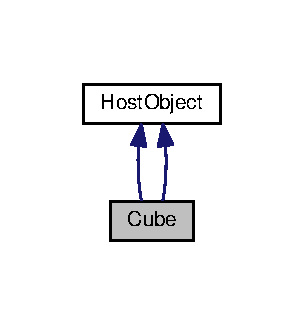
\includegraphics[width=146pt]{class_cube__inherit__graph}
\end{center}
\end{figure}


Collaboration diagram for Cube\+:
\nopagebreak
\begin{figure}[H]
\begin{center}
\leavevmode
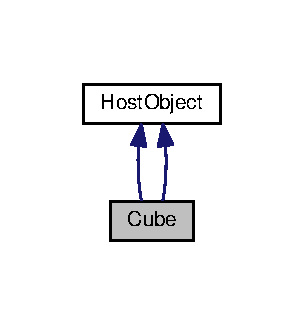
\includegraphics[width=146pt]{class_cube__coll__graph}
\end{center}
\end{figure}
\subsection*{Public Member Functions}
\begin{DoxyCompactItemize}
\item 
\+\_\+\+\_\+host\+\_\+\+\_\+ \+\_\+\+\_\+device\+\_\+\+\_\+ {\bfseries Cube} (const \hyperlink{class_vec3}{Vec3f} \&vmin, const \hyperlink{class_vec3}{Vec3f} \&vmax)\hypertarget{class_cube_a2ddff6f7a6270913135aaf3631d5c47f}{}\label{class_cube_a2ddff6f7a6270913135aaf3631d5c47f}

\item 
\+\_\+\+\_\+host\+\_\+\+\_\+ \+\_\+\+\_\+device\+\_\+\+\_\+ const \hyperlink{class_vec3}{Vec3f} \& {\bfseries operator\mbox{[}$\,$\mbox{]}} (uint8\+\_\+t i) const\hypertarget{class_cube_ae4abe305069b6d146155246f0e267250}{}\label{class_cube_ae4abe305069b6d146155246f0e267250}

\item 
\+\_\+\+\_\+host\+\_\+\+\_\+ \+\_\+\+\_\+device\+\_\+\+\_\+ \hyperlink{class_vec3}{Vec3f} \& {\bfseries operator\mbox{[}$\,$\mbox{]}} (uint8\+\_\+t i)\hypertarget{class_cube_a3f54f6e6398d0c0bb7fecb211129f5a0}{}\label{class_cube_a3f54f6e6398d0c0bb7fecb211129f5a0}

\item 
\+\_\+\+\_\+host\+\_\+\+\_\+ \+\_\+\+\_\+device\+\_\+\+\_\+ const \hyperlink{class_vec3}{Vec3f} \& {\bfseries min} () const\hypertarget{class_cube_ab027298d0436ab19e9376fb6a87ec4a9}{}\label{class_cube_ab027298d0436ab19e9376fb6a87ec4a9}

\item 
\+\_\+\+\_\+host\+\_\+\+\_\+ \+\_\+\+\_\+device\+\_\+\+\_\+ const \hyperlink{class_vec3}{Vec3f} \& {\bfseries max} () const\hypertarget{class_cube_abe52067f2ab40897e3cc41c287fd725c}{}\label{class_cube_abe52067f2ab40897e3cc41c287fd725c}

\item 
\+\_\+\+\_\+host\+\_\+\+\_\+ \+\_\+\+\_\+device\+\_\+\+\_\+ const \hyperlink{class_vec3}{Vec3f} \& {\bfseries normal} (uint8\+\_\+t plane\+Index) const\hypertarget{class_cube_acb0ccb67b7bc766d2a842a800859f3c0}{}\label{class_cube_acb0ccb67b7bc766d2a842a800859f3c0}

\item 
\+\_\+\+\_\+host\+\_\+\+\_\+ \+\_\+\+\_\+device\+\_\+\+\_\+ int {\bfseries v\+Index} (int plane\+Index, int element) const\hypertarget{class_cube_a5bb5ee3421c5f40ff5c71a849b0777bf}{}\label{class_cube_a5bb5ee3421c5f40ff5c71a849b0777bf}

\item 
\hyperlink{struct_polymorphic}{Polymorphic} {\bfseries get\+Device\+Polymorphic} (const Pattern \&dev\+\_\+pattern) const\hypertarget{class_cube_a91b7f2d2323140cfedbd92c61b636e56}{}\label{class_cube_a91b7f2d2323140cfedbd92c61b636e56}

\item 
void $\ast$ {\bfseries get\+Object} ()\hypertarget{class_cube_a9e68554bff4a2880f2ec981d2f8cb61a}{}\label{class_cube_a9e68554bff4a2880f2ec981d2f8cb61a}

\item 
size\+\_\+t {\bfseries bytes} () const\hypertarget{class_cube_a6dd4277f8d5956f74d73bb1ef988ae3a}{}\label{class_cube_a6dd4277f8d5956f74d73bb1ef988ae3a}

\item 
size\+\_\+t {\bfseries get\+Verts\+Number} () const\hypertarget{class_cube_a5cc25a88ab64cccb175db6f91241d92e}{}\label{class_cube_a5cc25a88ab64cccb175db6f91241d92e}

\item 
\+\_\+\+\_\+host\+\_\+\+\_\+ \+\_\+\+\_\+device\+\_\+\+\_\+ {\bfseries Cube} (const \hyperlink{class_vec3}{Vec3f} \&vmin, const \hyperlink{class_vec3}{Vec3f} \&vmax)\hypertarget{class_cube_a2ddff6f7a6270913135aaf3631d5c47f}{}\label{class_cube_a2ddff6f7a6270913135aaf3631d5c47f}

\item 
\+\_\+\+\_\+host\+\_\+\+\_\+ \+\_\+\+\_\+device\+\_\+\+\_\+ const \hyperlink{class_vec3}{Vec3f} \& {\bfseries operator\mbox{[}$\,$\mbox{]}} (uint8\+\_\+t i) const\hypertarget{class_cube_af8b0f76d2d1776fb9de4df6b7ee6a3ad}{}\label{class_cube_af8b0f76d2d1776fb9de4df6b7ee6a3ad}

\item 
\+\_\+\+\_\+host\+\_\+\+\_\+ \+\_\+\+\_\+device\+\_\+\+\_\+ \hyperlink{class_vec3}{Vec3f} \& {\bfseries operator\mbox{[}$\,$\mbox{]}} (uint8\+\_\+t i)\hypertarget{class_cube_a461bb6acf329d5863890be583c8f1ddc}{}\label{class_cube_a461bb6acf329d5863890be583c8f1ddc}

\item 
\+\_\+\+\_\+host\+\_\+\+\_\+ \+\_\+\+\_\+device\+\_\+\+\_\+ const \hyperlink{class_vec3}{Vec3f} \& {\bfseries min} () const\hypertarget{class_cube_aa9fbc346ac23564a2aba2ee5baed7f17}{}\label{class_cube_aa9fbc346ac23564a2aba2ee5baed7f17}

\item 
\+\_\+\+\_\+host\+\_\+\+\_\+ \+\_\+\+\_\+device\+\_\+\+\_\+ const \hyperlink{class_vec3}{Vec3f} \& {\bfseries max} () const\hypertarget{class_cube_a6169e4698259d8fcd5fc0825bca81359}{}\label{class_cube_a6169e4698259d8fcd5fc0825bca81359}

\item 
\+\_\+\+\_\+host\+\_\+\+\_\+ \+\_\+\+\_\+device\+\_\+\+\_\+ const \hyperlink{class_vec3}{Vec3f} \& {\bfseries normal} (uint8\+\_\+t plane\+Index) const\hypertarget{class_cube_aaff58267b0dcda266d9ef4ca620bb580}{}\label{class_cube_aaff58267b0dcda266d9ef4ca620bb580}

\item 
\+\_\+\+\_\+host\+\_\+\+\_\+ \+\_\+\+\_\+device\+\_\+\+\_\+ int {\bfseries v\+Index} (int plane\+Index, int element) const\hypertarget{class_cube_a5bb5ee3421c5f40ff5c71a849b0777bf}{}\label{class_cube_a5bb5ee3421c5f40ff5c71a849b0777bf}

\item 
\hyperlink{struct_polymorphic}{Polymorphic} {\bfseries get\+Device\+Polymorphic} (const Pattern \&dev\+\_\+pattern) const\hypertarget{class_cube_a91b7f2d2323140cfedbd92c61b636e56}{}\label{class_cube_a91b7f2d2323140cfedbd92c61b636e56}

\item 
void $\ast$ {\bfseries get\+Object} ()\hypertarget{class_cube_abc09a66095f46d824a78cca265e25ed5}{}\label{class_cube_abc09a66095f46d824a78cca265e25ed5}

\item 
size\+\_\+t {\bfseries bytes} () const\hypertarget{class_cube_a6dd4277f8d5956f74d73bb1ef988ae3a}{}\label{class_cube_a6dd4277f8d5956f74d73bb1ef988ae3a}

\item 
size\+\_\+t {\bfseries get\+Verts\+Number} () const\hypertarget{class_cube_a5cc25a88ab64cccb175db6f91241d92e}{}\label{class_cube_a5cc25a88ab64cccb175db6f91241d92e}

\end{DoxyCompactItemize}
\subsection*{Static Public Attributes}
\begin{DoxyCompactItemize}
\item 
static const uint8\+\_\+t {\bfseries verts\+Number} = 8\hypertarget{class_cube_a3b7080965552fbd2cae0bb0c3951de87}{}\label{class_cube_a3b7080965552fbd2cae0bb0c3951de87}

\item 
static const uint8\+\_\+t {\bfseries planes} = 6\hypertarget{class_cube_a0b3de7a2bec544a46c8d61e331637c6f}{}\label{class_cube_a0b3de7a2bec544a46c8d61e331637c6f}

\end{DoxyCompactItemize}


The documentation for this class was generated from the following files\+:\begin{DoxyCompactItemize}
\item 
/home/god/cuda-\/workspace/r\+T\+Tracer/include/object\+Box.\+cuh\item 
/home/god/cuda-\/workspace/r\+T\+Tracer/include/geometry\+Loader.\+cuh\item 
/home/god/cuda-\/workspace/r\+T\+Tracer/source/object\+Box.\+cu\end{DoxyCompactItemize}

\hypertarget{class_cuda_exception}{}\section{Cuda\+Exception Class Reference}
\label{class_cuda_exception}\index{Cuda\+Exception@{Cuda\+Exception}}


Inheritance diagram for Cuda\+Exception\+:
\nopagebreak
\begin{figure}[H]
\begin{center}
\leavevmode
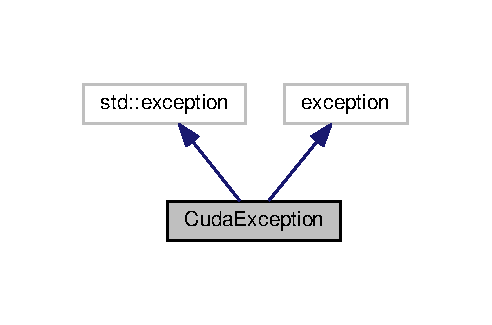
\includegraphics[width=163pt]{class_cuda_exception__inherit__graph}
\end{center}
\end{figure}


Collaboration diagram for Cuda\+Exception\+:
\nopagebreak
\begin{figure}[H]
\begin{center}
\leavevmode
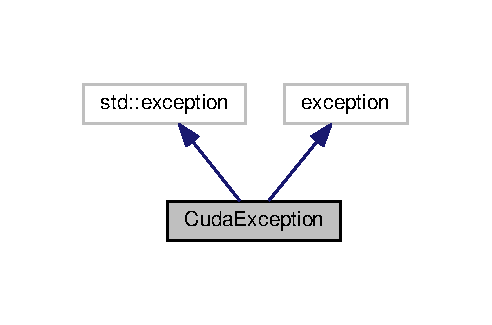
\includegraphics[width=163pt]{class_cuda_exception__coll__graph}
\end{center}
\end{figure}
\subsection*{Public Member Functions}
\begin{DoxyCompactItemize}
\item 
{\bfseries Cuda\+Exception} (std\+::string \&str)\hypertarget{class_cuda_exception_a17f8e85766f624c09c901bcdd79d7042}{}\label{class_cuda_exception_a17f8e85766f624c09c901bcdd79d7042}

\item 
{\bfseries Cuda\+Exception} (const char $\ast$str)\hypertarget{class_cuda_exception_a0d89dc2c59c4b25590ed463554af284d}{}\label{class_cuda_exception_a0d89dc2c59c4b25590ed463554af284d}

\item 
\hyperlink{class_cuda_exception}{Cuda\+Exception} \& {\bfseries operator+} (const std\+::exception \&e)\hypertarget{class_cuda_exception_acf9ac22baa0064c2e2d44faa222324b4}{}\label{class_cuda_exception_acf9ac22baa0064c2e2d44faa222324b4}

\item 
const char $\ast$ {\bfseries what} () const noexcept\hypertarget{class_cuda_exception_a5392d02d126a57a15cef5ff922ecbe3b}{}\label{class_cuda_exception_a5392d02d126a57a15cef5ff922ecbe3b}

\end{DoxyCompactItemize}


The documentation for this class was generated from the following file\+:\begin{DoxyCompactItemize}
\item 
/home/god/cuda-\/workspace/r\+T\+Tracer/include/helper.\+cuh\end{DoxyCompactItemize}

\hypertarget{class_dev_object}{}\section{Dev\+Object Class Reference}
\label{class_dev_object}\index{Dev\+Object@{Dev\+Object}}


Wrapper class for dynamic polymorphism on the device side.  




Collaboration diagram for Dev\+Object\+:
\nopagebreak
\begin{figure}[H]
\begin{center}
\leavevmode
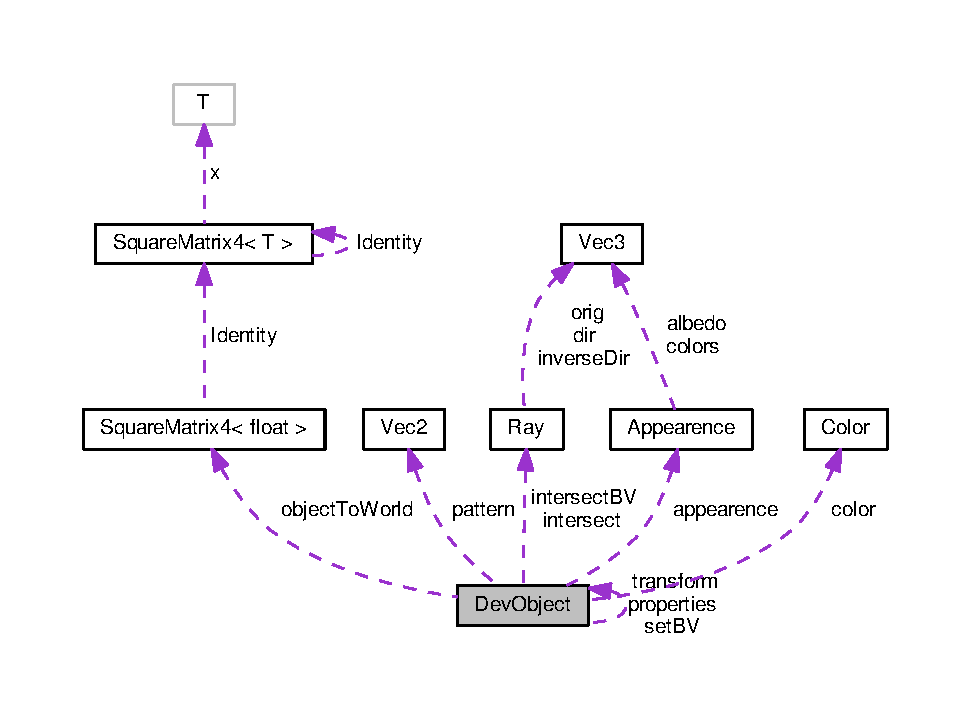
\includegraphics[width=350pt]{class_dev_object__coll__graph}
\end{center}
\end{figure}
\subsection*{Public Member Functions}
\begin{DoxyCompactItemize}
\item 
\+\_\+\+\_\+host\+\_\+\+\_\+ \+\_\+\+\_\+device\+\_\+\+\_\+ {\bfseries Dev\+Object} (const \hyperlink{class_dev_object}{Dev\+Object} \&object)\hypertarget{class_dev_object_a0eb5ac616858ccb98c7f9d0d6b136e37}{}\label{class_dev_object_a0eb5ac616858ccb98c7f9d0d6b136e37}

\item 
\+\_\+\+\_\+host\+\_\+\+\_\+ \+\_\+\+\_\+device\+\_\+\+\_\+ {\bfseries Dev\+Object} (uint32\+\_\+t verts\+Number, const \hyperlink{struct_appearence}{Appearence} \&appearence)\hypertarget{class_dev_object_a8a2f767cf3ef43bd298777d0c832a020}{}\label{class_dev_object_a8a2f767cf3ef43bd298777d0c832a020}

\item 
\+\_\+\+\_\+host\+\_\+\+\_\+ \+\_\+\+\_\+device\+\_\+\+\_\+ {\bfseries Dev\+Object} (const \hyperlink{struct_appearence}{Appearence} \&appearence)\hypertarget{class_dev_object_ac209dfe2089d0bc1b581d8437d9957a9}{}\label{class_dev_object_ac209dfe2089d0bc1b581d8437d9957a9}

\item 
\+\_\+\+\_\+host\+\_\+\+\_\+ \+\_\+\+\_\+device\+\_\+\+\_\+ \hyperlink{class_dev_object}{Dev\+Object} \& {\bfseries operator=} (const \hyperlink{class_dev_object}{Dev\+Object} \&object)\hypertarget{class_dev_object_a2ebee898cc6649365e984ae1b778a4f1}{}\label{class_dev_object_a2ebee898cc6649365e984ae1b778a4f1}

\item 
{\footnotesize template$<$class Object\+Type , class Bounding\+Volume\+Type $>$ }\\void {\bfseries init} (\hyperlink{struct_polymorphic}{Polymorphic} \&functions, void($\ast$destr)(\hyperlink{class_dev_object}{Dev\+Object} $\ast$), const Object\+Type $\ast$obj, Bounding\+Volume\+Type $\ast$$\ast$bv)\hypertarget{class_dev_object_a4eba0664c29dc32891f074b664e7d52d}{}\label{class_dev_object_a4eba0664c29dc32891f074b664e7d52d}

\item 
void {\bfseries init} (const \hyperlink{class_host_object}{Host\+Object} $\ast$obj, \hyperlink{class_boundaries}{Boundaries} $\ast$$\ast$bv, \hyperlink{struct_polymorphic}{Polymorphic} \&functions, void($\ast$destr)(\hyperlink{class_dev_object}{Dev\+Object} $\ast$))\hypertarget{class_dev_object_a71a495db8891a7a000e70fbd70876f9c}{}\label{class_dev_object_a71a495db8891a7a000e70fbd70876f9c}

\item 
\+\_\+\+\_\+host\+\_\+\+\_\+ \+\_\+\+\_\+device\+\_\+\+\_\+ const void $\ast$ {\bfseries data} () const\hypertarget{class_dev_object_a5533321471ee0ee776e30594ed48379f}{}\label{class_dev_object_a5533321471ee0ee776e30594ed48379f}

\item 
\+\_\+\+\_\+host\+\_\+\+\_\+ \+\_\+\+\_\+device\+\_\+\+\_\+ void $\ast$ {\bfseries data} ()\hypertarget{class_dev_object_a5335f7fb1dd5d15622aff5a8e9b0dc12}{}\label{class_dev_object_a5335f7fb1dd5d15622aff5a8e9b0dc12}

\item 
\+\_\+\+\_\+host\+\_\+\+\_\+ \+\_\+\+\_\+device\+\_\+\+\_\+ const \hyperlink{class_vec3}{Vec3f} \& {\bfseries albedo} () const\hypertarget{class_dev_object_ac4d2c0fc90a7be3085697e914bacc4d8}{}\label{class_dev_object_ac4d2c0fc90a7be3085697e914bacc4d8}

\item 
\+\_\+\+\_\+host\+\_\+\+\_\+ \+\_\+\+\_\+device\+\_\+\+\_\+ const void $\ast$ {\bfseries boundaries} () const\hypertarget{class_dev_object_a588ddd69ed74bc886b89fd4864024732}{}\label{class_dev_object_a588ddd69ed74bc886b89fd4864024732}

\item 
\+\_\+\+\_\+host\+\_\+\+\_\+ \+\_\+\+\_\+device\+\_\+\+\_\+ void {\bfseries swap} (\hyperlink{class_dev_object}{Dev\+Object} \&object)\hypertarget{class_dev_object_a56cf3cfc311cfe04da3b45f80e36625e}{}\label{class_dev_object_a56cf3cfc311cfe04da3b45f80e36625e}

\end{DoxyCompactItemize}
\subsection*{Public Attributes}
\begin{DoxyCompactItemize}
\item 
\hyperlink{struct_appearence}{Appearence} {\bfseries appearence}\hypertarget{class_dev_object_a6d67777a0bde8068561b3f3e2998f684}{}\label{class_dev_object_a6d67777a0bde8068561b3f3e2998f684}

\item 
uint32\+\_\+t {\bfseries verts\+Number}\hypertarget{class_dev_object_a934390fb2acf6be57335c1c17330f418}{}\label{class_dev_object_a934390fb2acf6be57335c1c17330f418}

\item 
Intersect {\bfseries intersect}\hypertarget{class_dev_object_ac461684d9baa47897b06b772ec1c5b6a}{}\label{class_dev_object_ac461684d9baa47897b06b772ec1c5b6a}

\item 
Intersect\+BV {\bfseries intersect\+BV}\hypertarget{class_dev_object_abb8de736d2e516ff0fad56413808c9e7}{}\label{class_dev_object_abb8de736d2e516ff0fad56413808c9e7}

\item 
Properties {\bfseries properties}\hypertarget{class_dev_object_aed644a97c45d96a4572a0f31f00e9d58}{}\label{class_dev_object_aed644a97c45d96a4572a0f31f00e9d58}

\item 
Transform {\bfseries transform}\hypertarget{class_dev_object_aba3965e5aa585859c53e81e8bd117a54}{}\label{class_dev_object_aba3965e5aa585859c53e81e8bd117a54}

\item 
Set\+BV {\bfseries set\+BV}\hypertarget{class_dev_object_ac6f9ceac5a6cdbc1f5513135cfe86e7f}{}\label{class_dev_object_ac6f9ceac5a6cdbc1f5513135cfe86e7f}

\item 
Pattern {\bfseries pattern}\hypertarget{class_dev_object_a383f8f80b90b69b98cbbc164b6905ae9}{}\label{class_dev_object_a383f8f80b90b69b98cbbc164b6905ae9}

\item 
void($\ast$ {\bfseries destructor} )(\hyperlink{class_dev_object}{Dev\+Object} $\ast$)\hypertarget{class_dev_object_aa16680d7d6b5526d5cde85c9e8d6aee3}{}\label{class_dev_object_aa16680d7d6b5526d5cde85c9e8d6aee3}

\item 
\hyperlink{class_square_matrix4}{Square\+Matrix4f} {\bfseries object\+To\+World}\hypertarget{class_dev_object_a7de79f32f1d5f9e1d5fcfa63a21c203b}{}\label{class_dev_object_a7de79f32f1d5f9e1d5fcfa63a21c203b}

\end{DoxyCompactItemize}
\subsection*{Protected Attributes}
\begin{DoxyCompactItemize}
\item 
void $\ast$ {\bfseries \+\_\+data}\hypertarget{class_dev_object_a362a69178014a44d0179e0ff07e70be9}{}\label{class_dev_object_a362a69178014a44d0179e0ff07e70be9}

\item 
void $\ast$ {\bfseries \+\_\+boundaries}\hypertarget{class_dev_object_a8f034e3a80c5a29de6e2f0fc190cb267}{}\label{class_dev_object_a8f034e3a80c5a29de6e2f0fc190cb267}

\item 
\hyperlink{class_color}{Color} {\bfseries color}\hypertarget{class_dev_object_a00c4791a548e2f1a45493bc3cbefba6a}{}\label{class_dev_object_a00c4791a548e2f1a45493bc3cbefba6a}

\end{DoxyCompactItemize}


\subsection{Detailed Description}
Wrapper class for dynamic polymorphism on the device side. 

The documentation for this class was generated from the following files\+:\begin{DoxyCompactItemize}
\item 
/home/god/cuda-\/workspace/r\+T\+Tracer/include/object\+Box.\+cuh\item 
/home/god/cuda-\/workspace/r\+T\+Tracer/source/object\+Box.\+cu\end{DoxyCompactItemize}

\hypertarget{class_distant_light}{}\section{Distant\+Light$<$ Direction\+Type $>$ Class Template Reference}
\label{class_distant_light}\index{Distant\+Light$<$ Direction\+Type $>$@{Distant\+Light$<$ Direction\+Type $>$}}
\subsection*{Public Member Functions}
\begin{DoxyCompactItemize}
\item 
\+\_\+\+\_\+host\+\_\+\+\_\+ \+\_\+\+\_\+device\+\_\+\+\_\+ {\bfseries Distant\+Light} (const \hyperlink{class_square_matrix4}{Square\+Matrix4f} \&model)\hypertarget{class_distant_light_a3565f9a26a0a865abf37c72ed63a7286}{}\label{class_distant_light_a3565f9a26a0a865abf37c72ed63a7286}

\item 
\+\_\+\+\_\+host\+\_\+\+\_\+ \+\_\+\+\_\+device\+\_\+\+\_\+ {\bfseries Distant\+Light} (const \hyperlink{class_square_matrix4}{Square\+Matrix4f} \&model)\hypertarget{class_distant_light_a3565f9a26a0a865abf37c72ed63a7286}{}\label{class_distant_light_a3565f9a26a0a865abf37c72ed63a7286}

\end{DoxyCompactItemize}
\subsection*{Public Attributes}
\begin{DoxyCompactItemize}
\item 
Direction\+Type {\bfseries dir}\hypertarget{class_distant_light_a6931acb5c11fddc6a6ea27091ca7c95f}{}\label{class_distant_light_a6931acb5c11fddc6a6ea27091ca7c95f}

\end{DoxyCompactItemize}


\subsection{Detailed Description}
\subsubsection*{template$<$typename Direction\+Type$>$\\*
class Distant\+Light$<$ Direction\+Type $>$}

Distant lights (sun light for example) -- emitted rays are parallel to each other.~\newline
 -\/\+Requires only a direction.~\newline
 -\/\+Affected by rotation~\newline
 -\/\+Unaffected by translation.~\newline


The documentation for this class was generated from the following file\+:\begin{DoxyCompactItemize}
\item 
/home/god/cuda-\/workspace/r\+T\+Tracer/include/light.\+cuh\end{DoxyCompactItemize}

\hypertarget{class_geometry_loader}{}\section{Geometry\+Loader$<$ Objects\+Type, Bounding\+Volume\+Type $>$ Class Template Reference}
\label{class_geometry_loader}\index{Geometry\+Loader$<$ Objects\+Type, Bounding\+Volume\+Type $>$@{Geometry\+Loader$<$ Objects\+Type, Bounding\+Volume\+Type $>$}}


Collaboration diagram for Geometry\+Loader$<$ Objects\+Type, Bounding\+Volume\+Type $>$\+:
\nopagebreak
\begin{figure}[H]
\begin{center}
\leavevmode
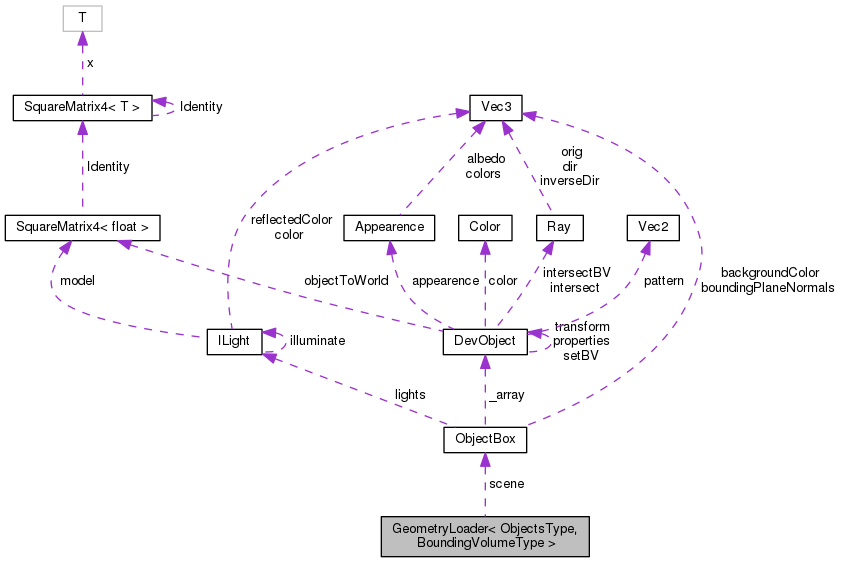
\includegraphics[width=350pt]{class_geometry_loader__coll__graph}
\end{center}
\end{figure}
\subsection*{Public Member Functions}
\begin{DoxyCompactItemize}
\item 
{\bfseries Geometry\+Loader} (const \hyperlink{class_geometry_loader}{Geometry\+Loader} \&utilities)\hypertarget{class_geometry_loader_a9c9114a5b074611c21bed13b4a4e5020}{}\label{class_geometry_loader_a9c9114a5b074611c21bed13b4a4e5020}

\item 
\hyperlink{class_geometry_loader_acdbb37e0f355aec4bd1c43315ca062de}{Geometry\+Loader} (const std\+::vector$<$ std\+::string $>$ \&filenames, const std\+::vector$<$ \hyperlink{class_square_matrix4}{Square\+Matrix4f} $>$ \&model, const std\+::vector$<$ \hyperlink{class_i_light}{I\+Light} $>$ \&lights, const std\+::vector$<$ \hyperlink{struct_appearence}{Appearence} $>$ \&appearences)
\item 
\hyperlink{class_geometry_loader_ad1e31702fc39f0fcc216beca12967872}{Geometry\+Loader} (const std\+::vector$<$ \hyperlink{class_i_light}{I\+Light} $>$ \&lights)
\item 
{\bfseries Geometry\+Loader} (const std\+::vector$<$ std\+::unique\+\_\+ptr$<$ \hyperlink{class_host_object}{Host\+Object} $>$$>$ \&host\+\_\+obj, const std\+::vector$<$ \hyperlink{class_i_light}{I\+Light} $>$ \&lights, const std\+::vector$<$ \hyperlink{struct_appearence}{Appearence} $>$ \&appearences)\hypertarget{class_geometry_loader_a0fba129ffcc51352ce49d22d30e83732}{}\label{class_geometry_loader_a0fba129ffcc51352ce49d22d30e83732}

\item 
\hyperlink{class_object_box}{Object\+Box} \& \hyperlink{class_geometry_loader_a99722ce01101349a6c792e87cc488d36}{operator()} (const \hyperlink{class_square_matrix4}{Square\+Matrix4f} \&transform, const int \&begin=0, const int \&end=1)
\item 
\hyperlink{class_object_box}{Object\+Box} \& \hyperlink{class_geometry_loader_a71c1d727c3939d3e4de530d8a4504687}{operator()} (int object\+Number)
\item 
void \hyperlink{class_geometry_loader_a41504f514cf9aed65d385e401ae2de22}{load\+Meshes} (const std\+::vector$<$ std\+::string $>$ \&filenames)
\item 
void \hyperlink{class_geometry_loader_ae12a7d2e1dddd53e79cf42edf7ce59d6}{run\+Demo} ()
\item 
void \hyperlink{class_geometry_loader_a9ee90083c2f62768f8a2c613fdcf0715}{pack\+Mesh} ()\hypertarget{class_geometry_loader_a9ee90083c2f62768f8a2c613fdcf0715}{}\label{class_geometry_loader_a9ee90083c2f62768f8a2c613fdcf0715}

\begin{DoxyCompactList}\small\item\em Function copies meshes to device memory and initializes wrapper objects. \end{DoxyCompactList}\item 
{\footnotesize template$<$class Procedural\+Object\+Type $>$ }\\void \hyperlink{class_geometry_loader_a175f8a4496b0b4d183f8eba7a2ac38f9}{pack\+Procedural} (const Procedural\+Object\+Type \&object, const \hyperlink{struct_polymorphic}{Polymorphic} \&functions, const \hyperlink{struct_appearence}{Appearence} \&appearence)
\begin{DoxyCompactList}\small\item\em Function copies implicit objects to device memory and initializes wrapper objects. \end{DoxyCompactList}\item 
void {\bfseries pack\+Procedural} (const \hyperlink{struct_polymorphic}{Polymorphic} \&functions, const \hyperlink{struct_appearence}{Appearence} \&appearence, const \hyperlink{class_host_object}{Host\+Object} \&object)\hypertarget{class_geometry_loader_a1d2eddd9fd6dfd98435ca4c2d618449e}{}\label{class_geometry_loader_a1d2eddd9fd6dfd98435ca4c2d618449e}

\item 
void \hyperlink{class_geometry_loader_a11a589427dc744b17ccc5085ec07a338}{pack\+Scene} ()\hypertarget{class_geometry_loader_a11a589427dc744b17ccc5085ec07a338}{}\label{class_geometry_loader_a11a589427dc744b17ccc5085ec07a338}

\begin{DoxyCompactList}\small\item\em Function wrapper objects and light objects to the \hyperlink{class_object_box}{Object\+Box} instance. \end{DoxyCompactList}\item 
\hyperlink{class_object_box}{Object\+Box} \& \hyperlink{class_geometry_loader_af3716f894c24e1662ffbbd48e0575bcd}{get} ()
\end{DoxyCompactItemize}
\subsection*{Public Attributes}
\begin{DoxyCompactItemize}
\item 
\hyperlink{class_object_box}{Object\+Box} {\bfseries scene}\hypertarget{class_geometry_loader_a3e040be4450444adddd72735905cb38e}{}\label{class_geometry_loader_a3e040be4450444adddd72735905cb38e}

\end{DoxyCompactItemize}


\subsection{Constructor \& Destructor Documentation}
\index{Geometry\+Loader@{Geometry\+Loader}!Geometry\+Loader@{Geometry\+Loader}}
\index{Geometry\+Loader@{Geometry\+Loader}!Geometry\+Loader@{Geometry\+Loader}}
\subsubsection[{\texorpdfstring{Geometry\+Loader(const std\+::vector$<$ std\+::string $>$ \&filenames, const std\+::vector$<$ Square\+Matrix4f $>$ \&model, const std\+::vector$<$ I\+Light $>$ \&lights, const std\+::vector$<$ Appearence $>$ \&appearences)}{GeometryLoader(const std::vector< std::string > \&filenames, const std::vector< SquareMatrix4f > \&model, const std::vector< ILight > \&lights, const std::vector< Appearence > \&appearences)}}]{\setlength{\rightskip}{0pt plus 5cm}template$<$class Objects\+Type, class Bounding\+Volume\+Type$>$ {\bf Geometry\+Loader}$<$ Objects\+Type, Bounding\+Volume\+Type $>$\+::{\bf Geometry\+Loader} (
\begin{DoxyParamCaption}
\item[{const std\+::vector$<$ std\+::string $>$ \&}]{filenames, }
\item[{const std\+::vector$<$ {\bf Square\+Matrix4f} $>$ \&}]{model, }
\item[{const std\+::vector$<$ {\bf I\+Light} $>$ \&}]{lights, }
\item[{const std\+::vector$<$ {\bf Appearence} $>$ \&}]{appearences}
\end{DoxyParamCaption}
)\hspace{0.3cm}{\ttfamily [inline]}}\hypertarget{class_geometry_loader_acdbb37e0f355aec4bd1c43315ca062de}{}\label{class_geometry_loader_acdbb37e0f355aec4bd1c43315ca062de}

\begin{DoxyParams}[1]{Parameters}
\mbox{\tt in}  & {\em -\/} & filenames -\/ storage for filenames with meshes. Each file must consist of the only one mesh. \\
\hline
\mbox{\tt in}  & {\em -\/} & model -\/ object-\/to-\/world matrix storage, each for every mesh transformation. \\
\hline
\mbox{\tt in}  & {\em -\/} & lights -\/ storage for lights of every implemented kind \\
\hline
\mbox{\tt in}  & {\em -\/} & appearences -\/ object shading properties \\
\hline
\end{DoxyParams}
\index{Geometry\+Loader@{Geometry\+Loader}!Geometry\+Loader@{Geometry\+Loader}}
\index{Geometry\+Loader@{Geometry\+Loader}!Geometry\+Loader@{Geometry\+Loader}}
\subsubsection[{\texorpdfstring{Geometry\+Loader(const std\+::vector$<$ I\+Light $>$ \&lights)}{GeometryLoader(const std::vector< ILight > \&lights)}}]{\setlength{\rightskip}{0pt plus 5cm}template$<$class Objects\+Type, class Bounding\+Volume\+Type$>$ {\bf Geometry\+Loader}$<$ Objects\+Type, Bounding\+Volume\+Type $>$\+::{\bf Geometry\+Loader} (
\begin{DoxyParamCaption}
\item[{const std\+::vector$<$ {\bf I\+Light} $>$ \&}]{lights}
\end{DoxyParamCaption}
)\hspace{0.3cm}{\ttfamily [inline]}}\hypertarget{class_geometry_loader_ad1e31702fc39f0fcc216beca12967872}{}\label{class_geometry_loader_ad1e31702fc39f0fcc216beca12967872}

\begin{DoxyParams}[1]{Parameters}
\mbox{\tt in}  & {\em lights} & -\/ storage for lights of every implemented kind \\
\hline
\end{DoxyParams}


\subsection{Member Function Documentation}
\index{Geometry\+Loader@{Geometry\+Loader}!get@{get}}
\index{get@{get}!Geometry\+Loader@{Geometry\+Loader}}
\subsubsection[{\texorpdfstring{get()}{get()}}]{\setlength{\rightskip}{0pt plus 5cm}template$<$class Objects\+Type, class Bounding\+Volume\+Type$>$ {\bf Object\+Box}\& {\bf Geometry\+Loader}$<$ Objects\+Type, Bounding\+Volume\+Type $>$\+::get (
\begin{DoxyParamCaption}
{}
\end{DoxyParamCaption}
)\hspace{0.3cm}{\ttfamily [inline]}}\hypertarget{class_geometry_loader_af3716f894c24e1662ffbbd48e0575bcd}{}\label{class_geometry_loader_af3716f894c24e1662ffbbd48e0575bcd}
\begin{DoxyReturn}{Returns}
\hyperlink{class_object_box}{Object\+Box} instance. 
\end{DoxyReturn}
\index{Geometry\+Loader@{Geometry\+Loader}!load\+Meshes@{load\+Meshes}}
\index{load\+Meshes@{load\+Meshes}!Geometry\+Loader@{Geometry\+Loader}}
\subsubsection[{\texorpdfstring{load\+Meshes(const std\+::vector$<$ std\+::string $>$ \&filenames)}{loadMeshes(const std::vector< std::string > \&filenames)}}]{\setlength{\rightskip}{0pt plus 5cm}template$<$class Objects\+Type, class Bounding\+Volume\+Type$>$ void {\bf Geometry\+Loader}$<$ Objects\+Type, Bounding\+Volume\+Type $>$\+::load\+Meshes (
\begin{DoxyParamCaption}
\item[{const std\+::vector$<$ std\+::string $>$ \&}]{filenames}
\end{DoxyParamCaption}
)\hspace{0.3cm}{\ttfamily [inline]}}\hypertarget{class_geometry_loader_a41504f514cf9aed65d385e401ae2de22}{}\label{class_geometry_loader_a41504f514cf9aed65d385e401ae2de22}
Function loads meshes from file. 
\begin{DoxyParams}[1]{Parameters}
\mbox{\tt in}  & {\em filenames} & \\
\hline
\end{DoxyParams}
\index{Geometry\+Loader@{Geometry\+Loader}!operator()@{operator()}}
\index{operator()@{operator()}!Geometry\+Loader@{Geometry\+Loader}}
\subsubsection[{\texorpdfstring{operator()(const Square\+Matrix4f \&transform, const int \&begin=0, const int \&end=1)}{operator()(const SquareMatrix4f \&transform, const int \&begin=0, const int \&end=1)}}]{\setlength{\rightskip}{0pt plus 5cm}template$<$class Objects\+Type, class Bounding\+Volume\+Type$>$ {\bf Object\+Box}\& {\bf Geometry\+Loader}$<$ Objects\+Type, Bounding\+Volume\+Type $>$\+::operator() (
\begin{DoxyParamCaption}
\item[{const {\bf Square\+Matrix4f} \&}]{transform, }
\item[{const int \&}]{begin = {\ttfamily 0}, }
\item[{const int \&}]{end = {\ttfamily 1}}
\end{DoxyParamCaption}
)\hspace{0.3cm}{\ttfamily [inline]}}\hypertarget{class_geometry_loader_a99722ce01101349a6c792e87cc488d36}{}\label{class_geometry_loader_a99722ce01101349a6c792e87cc488d36}
1) Applies transformation matrix to the mesh vertices.~\newline
 2) Recomputes bounding boundaries. 
\begin{DoxyParams}[1]{Parameters}
\mbox{\tt in}  & {\em transform} & -\/ a new transformation matrix \\
\hline
\mbox{\tt in}  & {\em begin} & -\/ the first point to be transformed \\
\hline
\mbox{\tt in}  & {\em end} & -\/ the point after the last one \\
\hline
\end{DoxyParams}
\begin{DoxyReturn}{Returns}
-\/ \hyperlink{class_object_box}{Object\+Box} wrapper of new scene considering transformations 
\end{DoxyReturn}
\index{Geometry\+Loader@{Geometry\+Loader}!operator()@{operator()}}
\index{operator()@{operator()}!Geometry\+Loader@{Geometry\+Loader}}
\subsubsection[{\texorpdfstring{operator()(int object\+Number)}{operator()(int objectNumber)}}]{\setlength{\rightskip}{0pt plus 5cm}template$<$class Objects\+Type, class Bounding\+Volume\+Type$>$ {\bf Object\+Box}\& {\bf Geometry\+Loader}$<$ Objects\+Type, Bounding\+Volume\+Type $>$\+::operator() (
\begin{DoxyParamCaption}
\item[{int}]{object\+Number}
\end{DoxyParamCaption}
)\hspace{0.3cm}{\ttfamily [inline]}}\hypertarget{class_geometry_loader_a71c1d727c3939d3e4de530d8a4504687}{}\label{class_geometry_loader_a71c1d727c3939d3e4de530d8a4504687}
Function recomputes a bounding boundaries of a particular object. 
\begin{DoxyParams}[1]{Parameters}
\mbox{\tt in}  & {\em object\+Number} & \\
\hline
\end{DoxyParams}
\begin{DoxyReturn}{Returns}
\hyperlink{class_object_box}{Object\+Box} wrapper of new scene considering transformations 
\end{DoxyReturn}
\index{Geometry\+Loader@{Geometry\+Loader}!pack\+Procedural@{pack\+Procedural}}
\index{pack\+Procedural@{pack\+Procedural}!Geometry\+Loader@{Geometry\+Loader}}
\subsubsection[{\texorpdfstring{pack\+Procedural(const Procedural\+Object\+Type \&object, const Polymorphic \&functions, const Appearence \&appearence)}{packProcedural(const ProceduralObjectType \&object, const Polymorphic \&functions, const Appearence \&appearence)}}]{\setlength{\rightskip}{0pt plus 5cm}template$<$class Objects\+Type, class Bounding\+Volume\+Type$>$ template$<$class Procedural\+Object\+Type $>$ void {\bf Geometry\+Loader}$<$ Objects\+Type, Bounding\+Volume\+Type $>$\+::pack\+Procedural (
\begin{DoxyParamCaption}
\item[{const Procedural\+Object\+Type \&}]{object, }
\item[{const {\bf Polymorphic} \&}]{functions, }
\item[{const {\bf Appearence} \&}]{appearence}
\end{DoxyParamCaption}
)\hspace{0.3cm}{\ttfamily [inline]}}\hypertarget{class_geometry_loader_a175f8a4496b0b4d183f8eba7a2ac38f9}{}\label{class_geometry_loader_a175f8a4496b0b4d183f8eba7a2ac38f9}


Function copies implicit objects to device memory and initializes wrapper objects. 


\begin{DoxyParams}[1]{Parameters}
\mbox{\tt in}  & {\em object} & -\/ an instance of a particular object \\
\hline
\mbox{\tt in}  & {\em functions} & -\/ instance with static function pointers \\
\hline
\mbox{\tt in}  & {\em appearences} & -\/ object shading properties \\
\hline
\end{DoxyParams}
Here is the call graph for this function\+:
\nopagebreak
\begin{figure}[H]
\begin{center}
\leavevmode
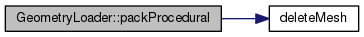
\includegraphics[width=345pt]{class_geometry_loader_a175f8a4496b0b4d183f8eba7a2ac38f9_cgraph}
\end{center}
\end{figure}
\index{Geometry\+Loader@{Geometry\+Loader}!run\+Demo@{run\+Demo}}
\index{run\+Demo@{run\+Demo}!Geometry\+Loader@{Geometry\+Loader}}
\subsubsection[{\texorpdfstring{run\+Demo()}{runDemo()}}]{\setlength{\rightskip}{0pt plus 5cm}template$<$class Objects\+Type, class Bounding\+Volume\+Type$>$ void {\bf Geometry\+Loader}$<$ Objects\+Type, Bounding\+Volume\+Type $>$\+::run\+Demo (
\begin{DoxyParamCaption}
{}
\end{DoxyParamCaption}
)\hspace{0.3cm}{\ttfamily [inline]}}\hypertarget{class_geometry_loader_ae12a7d2e1dddd53e79cf42edf7ce59d6}{}\label{class_geometry_loader_ae12a7d2e1dddd53e79cf42edf7ce59d6}
Function loads implicit objects. Here is the call graph for this function\+:
\nopagebreak
\begin{figure}[H]
\begin{center}
\leavevmode
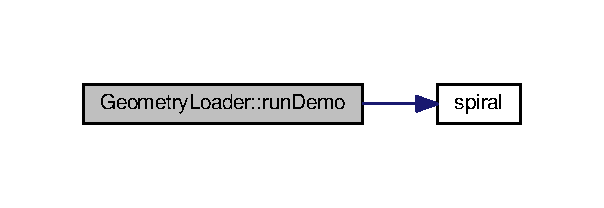
\includegraphics[width=290pt]{class_geometry_loader_ae12a7d2e1dddd53e79cf42edf7ce59d6_cgraph}
\end{center}
\end{figure}


The documentation for this class was generated from the following file\+:\begin{DoxyCompactItemize}
\item 
/home/god/cuda-\/workspace/r\+T\+Tracer/include/geometry\+Loader.\+cuh\end{DoxyCompactItemize}

\hypertarget{class_host_object}{}\section{Host\+Object Class Reference}
\label{class_host_object}\index{Host\+Object@{Host\+Object}}


Parent class for most of the class objects in the project except of \hyperlink{class_triangle}{Triangle} class.  




Inheritance diagram for Host\+Object\+:
\nopagebreak
\begin{figure}[H]
\begin{center}
\leavevmode
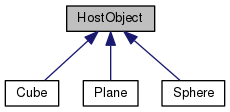
\includegraphics[width=245pt]{class_host_object__inherit__graph}
\end{center}
\end{figure}
\subsection*{Public Member Functions}
\begin{DoxyCompactItemize}
\item 
virtual \hyperlink{struct_polymorphic}{Polymorphic} {\bfseries get\+Device\+Polymorphic} (const Pattern \&dev\+\_\+pattern) const =0\hypertarget{class_host_object_a41171fd7c423b8b766d06f55fa4be867}{}\label{class_host_object_a41171fd7c423b8b766d06f55fa4be867}

\item 
virtual void $\ast$ {\bfseries get\+Object} ()=0\hypertarget{class_host_object_a32c392f12e133d9ecfce76a2e5135c94}{}\label{class_host_object_a32c392f12e133d9ecfce76a2e5135c94}

\item 
virtual size\+\_\+t {\bfseries bytes} () const =0\hypertarget{class_host_object_aacb8c44633ea4411d0972f933870557e}{}\label{class_host_object_aacb8c44633ea4411d0972f933870557e}

\item 
virtual size\+\_\+t {\bfseries get\+Verts\+Number} () const =0\hypertarget{class_host_object_a0d6005a4895a5246deae24daf2c71ca7}{}\label{class_host_object_a0d6005a4895a5246deae24daf2c71ca7}

\item 
virtual \hyperlink{struct_polymorphic}{Polymorphic} {\bfseries get\+Device\+Polymorphic} (const Pattern \&dev\+\_\+pattern) const =0\hypertarget{class_host_object_a41171fd7c423b8b766d06f55fa4be867}{}\label{class_host_object_a41171fd7c423b8b766d06f55fa4be867}

\item 
virtual void $\ast$ {\bfseries get\+Object} ()=0\hypertarget{class_host_object_a32c392f12e133d9ecfce76a2e5135c94}{}\label{class_host_object_a32c392f12e133d9ecfce76a2e5135c94}

\item 
virtual size\+\_\+t {\bfseries bytes} () const =0\hypertarget{class_host_object_aacb8c44633ea4411d0972f933870557e}{}\label{class_host_object_aacb8c44633ea4411d0972f933870557e}

\item 
virtual size\+\_\+t {\bfseries get\+Verts\+Number} () const =0\hypertarget{class_host_object_a0d6005a4895a5246deae24daf2c71ca7}{}\label{class_host_object_a0d6005a4895a5246deae24daf2c71ca7}

\end{DoxyCompactItemize}


\subsection{Detailed Description}
Parent class for most of the class objects in the project except of \hyperlink{class_triangle}{Triangle} class. 

The documentation for this class was generated from the following file\+:\begin{DoxyCompactItemize}
\item 
/home/god/cuda-\/workspace/r\+T\+Tracer/include/object\+Box.\+cuh\end{DoxyCompactItemize}

\hypertarget{class_i_light}{}\section{I\+Light Class Reference}
\label{class_i_light}\index{I\+Light@{I\+Light}}


Area lights.  




Collaboration diagram for I\+Light\+:
\nopagebreak
\begin{figure}[H]
\begin{center}
\leavevmode
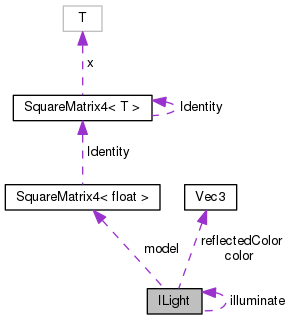
\includegraphics[width=291pt]{class_i_light__coll__graph}
\end{center}
\end{figure}
\subsection*{Public Member Functions}
\begin{DoxyCompactItemize}
\item 
\+\_\+\+\_\+host\+\_\+\+\_\+ \+\_\+\+\_\+device\+\_\+\+\_\+ {\bfseries I\+Light} (const \hyperlink{class_square_matrix4}{Square\+Matrix4f} \&l2w, const \hyperlink{class_vec3}{Vec3f} \&color, const float \&i, uint8\+\_\+t light\+Type)\hypertarget{class_i_light_aa788ba40470cbbd251cf06b9a80c7a77}{}\label{class_i_light_aa788ba40470cbbd251cf06b9a80c7a77}

\item 
\+\_\+\+\_\+host\+\_\+\+\_\+ \+\_\+\+\_\+device\+\_\+\+\_\+ {\bfseries I\+Light} (const \hyperlink{class_i_light}{I\+Light} \&light)\hypertarget{class_i_light_ae44c2228daf4c95f4df2fea3c50c8abf}{}\label{class_i_light_ae44c2228daf4c95f4df2fea3c50c8abf}

\item 
{\footnotesize template$<$class Light\+Type $>$ }\\void {\bfseries init} (Reflected\+Color \&rc, Illuminate \&illum)\hypertarget{class_i_light_a3c93b73052074a1dc80d6a18f027e8e1}{}\label{class_i_light_a3c93b73052074a1dc80d6a18f027e8e1}

\item 
{\footnotesize template$<$class Light\+Type $>$ }\\void {\bfseries dev\+Allocate\+Light} ()\hypertarget{class_i_light_a1c67d8cf9d7492c1ff61c156abaa0323}{}\label{class_i_light_a1c67d8cf9d7492c1ff61c156abaa0323}

\item 
\+\_\+\+\_\+host\+\_\+\+\_\+ \+\_\+\+\_\+device\+\_\+\+\_\+ \hyperlink{class_i_light}{I\+Light} \& {\bfseries operator=} (const \hyperlink{class_i_light}{I\+Light} \&light)\hypertarget{class_i_light_a9852bdb910c17654c08b76a9df20fd25}{}\label{class_i_light_a9852bdb910c17654c08b76a9df20fd25}

\item 
\+\_\+\+\_\+host\+\_\+\+\_\+ \+\_\+\+\_\+device\+\_\+\+\_\+ const void $\ast$ {\bfseries data} () const\hypertarget{class_i_light_aab75634731a67d8d1802044c34d1facd}{}\label{class_i_light_aab75634731a67d8d1802044c34d1facd}

\item 
\+\_\+\+\_\+host\+\_\+\+\_\+ \+\_\+\+\_\+device\+\_\+\+\_\+ void $\ast$ {\bfseries data} ()\hypertarget{class_i_light_ac22951f44f0e03cd4552cee51daad9f8}{}\label{class_i_light_ac22951f44f0e03cd4552cee51daad9f8}

\item 
\+\_\+\+\_\+host\+\_\+\+\_\+ \+\_\+\+\_\+device\+\_\+\+\_\+ {\bfseries I\+Light} (const \hyperlink{class_square_matrix4}{Square\+Matrix4f} \&l2w, const \hyperlink{class_vec3}{Vec3f} \&color, const float \&i, uint8\+\_\+t light\+Type)\hypertarget{class_i_light_a05c5ebb3f5acc921047915410d772672}{}\label{class_i_light_a05c5ebb3f5acc921047915410d772672}

\item 
\+\_\+\+\_\+host\+\_\+\+\_\+ \+\_\+\+\_\+device\+\_\+\+\_\+ {\bfseries I\+Light} (const \hyperlink{class_i_light}{I\+Light} \&light)\hypertarget{class_i_light_ae44c2228daf4c95f4df2fea3c50c8abf}{}\label{class_i_light_ae44c2228daf4c95f4df2fea3c50c8abf}

\item 
{\footnotesize template$<$class Light\+Type $>$ }\\void {\bfseries init} (Reflected\+Color \&rc, Illuminate \&illum)\hypertarget{class_i_light_a3c93b73052074a1dc80d6a18f027e8e1}{}\label{class_i_light_a3c93b73052074a1dc80d6a18f027e8e1}

\item 
{\footnotesize template$<$class Light\+Type $>$ }\\void {\bfseries dev\+Allocate\+Light} ()\hypertarget{class_i_light_a1c67d8cf9d7492c1ff61c156abaa0323}{}\label{class_i_light_a1c67d8cf9d7492c1ff61c156abaa0323}

\item 
\+\_\+\+\_\+host\+\_\+\+\_\+ \+\_\+\+\_\+device\+\_\+\+\_\+ \hyperlink{class_i_light}{I\+Light} \& {\bfseries operator=} (const \hyperlink{class_i_light}{I\+Light} \&light)\hypertarget{class_i_light_aa813302e695747a6a5280bda335e9632}{}\label{class_i_light_aa813302e695747a6a5280bda335e9632}

\item 
\+\_\+\+\_\+host\+\_\+\+\_\+ \+\_\+\+\_\+device\+\_\+\+\_\+ const void $\ast$ {\bfseries data} () const\hypertarget{class_i_light_a9c07907231ff944271f6dab6d88b1432}{}\label{class_i_light_a9c07907231ff944271f6dab6d88b1432}

\item 
\+\_\+\+\_\+host\+\_\+\+\_\+ \+\_\+\+\_\+device\+\_\+\+\_\+ void $\ast$ {\bfseries data} ()\hypertarget{class_i_light_ae49c0d8a0be349e28b9a0e0c6c2a9306}{}\label{class_i_light_ae49c0d8a0be349e28b9a0e0c6c2a9306}

\end{DoxyCompactItemize}
\subsection*{Public Attributes}
\begin{DoxyCompactItemize}
\item 
const uint8\+\_\+t {\bfseries light\+Type}\hypertarget{class_i_light_a592b1197728a9b0ca9628f34856cff45}{}\label{class_i_light_a592b1197728a9b0ca9628f34856cff45}

\item 
Illuminate {\bfseries illuminate}\hypertarget{class_i_light_ad5ad27cccb6e7826692fac29537d076f}{}\label{class_i_light_ad5ad27cccb6e7826692fac29537d076f}

\item 
Reflected\+Color {\bfseries reflected\+Color}\hypertarget{class_i_light_a95817a159b6785ce2a4c6173fff682a6}{}\label{class_i_light_a95817a159b6785ce2a4c6173fff682a6}

\item 
\hyperlink{class_vec3}{Vec3f} {\bfseries color}\hypertarget{class_i_light_a539825d74cc014ecbc4b4d9fdea4373a}{}\label{class_i_light_a539825d74cc014ecbc4b4d9fdea4373a}

\item 
float {\bfseries intensity}\hypertarget{class_i_light_a91736d3b866f370017c3d409dee239ef}{}\label{class_i_light_a91736d3b866f370017c3d409dee239ef}

\item 
\hyperlink{class_square_matrix4}{Square\+Matrix4f} {\bfseries model}\hypertarget{class_i_light_ae508549f5ec5b492c5f1a19df37e792b}{}\label{class_i_light_ae508549f5ec5b492c5f1a19df37e792b}

\end{DoxyCompactItemize}


\subsection{Detailed Description}
Area lights. 

The documentation for this class was generated from the following files\+:\begin{DoxyCompactItemize}
\item 
/home/god/cuda-\/workspace/r\+T\+Tracer/include/light.\+cuh\item 
/home/god/cuda-\/workspace/r\+T\+Tracer/source/light.\+cu\end{DoxyCompactItemize}

\hypertarget{class_mesh}{}\section{Mesh Class Reference}
\label{class_mesh}\index{Mesh@{Mesh}}


Class for triangulated mesh polygons.  




Collaboration diagram for Mesh\+:
\nopagebreak
\begin{figure}[H]
\begin{center}
\leavevmode
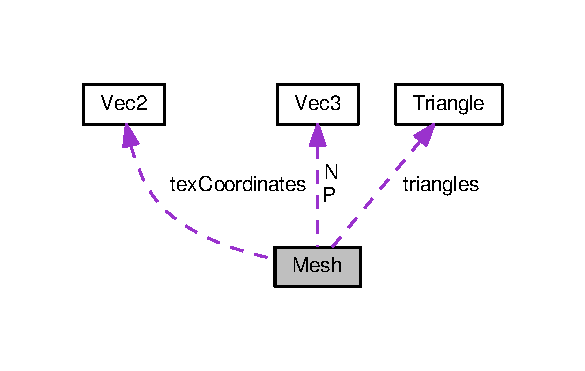
\includegraphics[width=281pt]{class_mesh__coll__graph}
\end{center}
\end{figure}
\subsection*{Public Member Functions}
\begin{DoxyCompactItemize}
\item 
{\bfseries Mesh} (const uint32\+\_\+t nfaces, const std\+::vector$<$ uint32\+\_\+t $>$ \&face\+Index, const std\+::vector$<$ uint32\+\_\+t $>$ \&verts\+Index, std\+::vector$<$ \hyperlink{class_vec3}{Vec3f} $>$ \&verts, const std\+::vector$<$ \hyperlink{class_vec3}{Vec3f} $>$ \&normals, const std\+::vector$<$ \hyperlink{class_vec2}{Vec2f} $>$ \&st, const \hyperlink{class_square_matrix4}{Square\+Matrix4f} \&model)\hypertarget{class_mesh_ae66d189c5755899fc40c0a6f33a28781}{}\label{class_mesh_ae66d189c5755899fc40c0a6f33a28781}

\item 
\+\_\+\+\_\+host\+\_\+\+\_\+ \+\_\+\+\_\+device\+\_\+\+\_\+ const \hyperlink{class_vec3}{Vec3f} \& {\bfseries operator\mbox{[}$\,$\mbox{]}} (size\+\_\+t i) const\hypertarget{class_mesh_abe7a4a30b9a82dd71164071d0f398ab8}{}\label{class_mesh_abe7a4a30b9a82dd71164071d0f398ab8}

\item 
\+\_\+\+\_\+host\+\_\+\+\_\+ \+\_\+\+\_\+device\+\_\+\+\_\+ \hyperlink{class_vec3}{Vec3f} \& {\bfseries operator\mbox{[}$\,$\mbox{]}} (size\+\_\+t i)\hypertarget{class_mesh_ad97c062c97725555f13cec4c9c00448f}{}\label{class_mesh_ad97c062c97725555f13cec4c9c00448f}

\item 
\hyperlink{struct_polymorphic}{Polymorphic} {\bfseries get\+Device\+Polymorphic} (const Pattern \&dev\+\_\+pattern)\hypertarget{class_mesh_a5a6b65787f239cffc60fbf955473b129}{}\label{class_mesh_a5a6b65787f239cffc60fbf955473b129}

\item 
\hyperlink{class_vec3}{Vec3f} $\ast$ {\bfseries data} ()\hypertarget{class_mesh_a827769cc062165859fc51581e14d64d8}{}\label{class_mesh_a827769cc062165859fc51581e14d64d8}

\item 
{\bfseries Mesh} (const uint32\+\_\+t nfaces, const std\+::vector$<$ uint32\+\_\+t $>$ \&face\+Index, const std\+::vector$<$ uint32\+\_\+t $>$ \&verts\+Index, std\+::vector$<$ \hyperlink{class_vec3}{Vec3f} $>$ \&verts, const std\+::vector$<$ \hyperlink{class_vec3}{Vec3f} $>$ \&normals, const std\+::vector$<$ \hyperlink{class_vec2}{Vec2f} $>$ \&st, const \hyperlink{class_square_matrix4}{Square\+Matrix4f} \&model)\hypertarget{class_mesh_ae66d189c5755899fc40c0a6f33a28781}{}\label{class_mesh_ae66d189c5755899fc40c0a6f33a28781}

\item 
\+\_\+\+\_\+host\+\_\+\+\_\+ \+\_\+\+\_\+device\+\_\+\+\_\+ const \hyperlink{class_vec3}{Vec3f} \& {\bfseries operator\mbox{[}$\,$\mbox{]}} (size\+\_\+t i) const\hypertarget{class_mesh_ace991bdeffafcf1d7d9ceaf6a697e6bd}{}\label{class_mesh_ace991bdeffafcf1d7d9ceaf6a697e6bd}

\item 
\+\_\+\+\_\+host\+\_\+\+\_\+ \+\_\+\+\_\+device\+\_\+\+\_\+ \hyperlink{class_vec3}{Vec3f} \& {\bfseries operator\mbox{[}$\,$\mbox{]}} (size\+\_\+t i)\hypertarget{class_mesh_a2fec73c82d262d4a5b09dc80918c1054}{}\label{class_mesh_a2fec73c82d262d4a5b09dc80918c1054}

\item 
\hyperlink{struct_polymorphic}{Polymorphic} {\bfseries get\+Device\+Polymorphic} (const Pattern \&dev\+\_\+pattern)\hypertarget{class_mesh_a5a6b65787f239cffc60fbf955473b129}{}\label{class_mesh_a5a6b65787f239cffc60fbf955473b129}

\item 
\hyperlink{class_vec3}{Vec3f} $\ast$ {\bfseries data} ()\hypertarget{class_mesh_a4974d2a092f0b34a0e4d0de0cf7f0bac}{}\label{class_mesh_a4974d2a092f0b34a0e4d0de0cf7f0bac}

\end{DoxyCompactItemize}
\subsection*{Public Attributes}
\begin{DoxyCompactItemize}
\item 
uint32\+\_\+t \hyperlink{class_mesh_a77cc0257fcf6e780b4d286a97e94ec3c}{verts\+Number}\hypertarget{class_mesh_a77cc0257fcf6e780b4d286a97e94ec3c}{}\label{class_mesh_a77cc0257fcf6e780b4d286a97e94ec3c}

\begin{DoxyCompactList}\small\item\em the maximum number of vertices \end{DoxyCompactList}\item 
uint32\+\_\+t \hyperlink{class_mesh_a6cf23eafd1fca3375dcd7ed805f32340}{num\+Tris}\hypertarget{class_mesh_a6cf23eafd1fca3375dcd7ed805f32340}{}\label{class_mesh_a6cf23eafd1fca3375dcd7ed805f32340}

\begin{DoxyCompactList}\small\item\em number of triangles \end{DoxyCompactList}\item 
\hyperlink{class_vec3}{Vec3f} $\ast$ {\bfseries P}\hypertarget{class_mesh_a977d73ff3b08961c0c7fea25897422d6}{}\label{class_mesh_a977d73ff3b08961c0c7fea25897422d6}

\item 
\hyperlink{class_triangle}{Triangle} $\ast$ {\bfseries triangles}\hypertarget{class_mesh_acfbc65d1fea728464f102eac4e6def71}{}\label{class_mesh_acfbc65d1fea728464f102eac4e6def71}

\item 
\hyperlink{class_vec3}{Vec3f} $\ast$ \hyperlink{class_mesh_a3f10793cd173995a7042acf97955984f}{N}\hypertarget{class_mesh_a3f10793cd173995a7042acf97955984f}{}\label{class_mesh_a3f10793cd173995a7042acf97955984f}

\begin{DoxyCompactList}\small\item\em triangles vertex normals \end{DoxyCompactList}\item 
\hyperlink{class_vec2}{Vec2f} $\ast$ \hyperlink{class_mesh_afa65cdda90551fad18f51c044e9a9b5e}{tex\+Coordinates}\hypertarget{class_mesh_afa65cdda90551fad18f51c044e9a9b5e}{}\label{class_mesh_afa65cdda90551fad18f51c044e9a9b5e}

\begin{DoxyCompactList}\small\item\em triangles texture coordinates \end{DoxyCompactList}\end{DoxyCompactItemize}


\subsection{Detailed Description}
Class for triangulated mesh polygons. 

The documentation for this class was generated from the following files\+:\begin{DoxyCompactItemize}
\item 
/home/god/cuda-\/workspace/r\+T\+Tracer/include/object\+Box.\+cuh\item 
/home/god/cuda-\/workspace/r\+T\+Tracer/include/geometry\+Loader.\+cuh\item 
/home/god/cuda-\/workspace/r\+T\+Tracer/source/object\+Box.\+cu\end{DoxyCompactItemize}

\hypertarget{class_mesh_transformation}{}\section{Mesh\+Transformation Class Reference}
\label{class_mesh_transformation}\index{Mesh\+Transformation@{Mesh\+Transformation}}


Inheritance diagram for Mesh\+Transformation\+:
\nopagebreak
\begin{figure}[H]
\begin{center}
\leavevmode
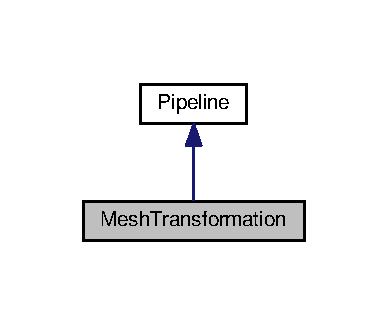
\includegraphics[width=186pt]{class_mesh_transformation__inherit__graph}
\end{center}
\end{figure}


Collaboration diagram for Mesh\+Transformation\+:
\nopagebreak
\begin{figure}[H]
\begin{center}
\leavevmode
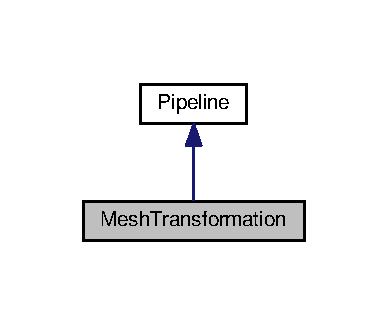
\includegraphics[width=186pt]{class_mesh_transformation__coll__graph}
\end{center}
\end{figure}
\subsection*{Public Member Functions}
\begin{DoxyCompactItemize}
\item 
float3 \hyperlink{class_mesh_transformation_a62b90b65ce289707982efdb23a88e517}{normalize} (float3 axis) const
\item 
\hyperlink{class_square_matrix4}{Square\+Matrix4f} \hyperlink{class_mesh_transformation_afd48394eed82a85ca29d05cd4817c29e}{transform} () const\hypertarget{class_mesh_transformation_afd48394eed82a85ca29d05cd4817c29e}{}\label{class_mesh_transformation_afd48394eed82a85ca29d05cd4817c29e}

\begin{DoxyCompactList}\small\item\em The function is called after applying all the transformations. \end{DoxyCompactList}\item 
\hyperlink{class_square_matrix4}{Square\+Matrix4f} \& \hyperlink{class_mesh_transformation_ad14a09457c8d103682183cd8e13b78dc}{rotate} (const float3 \&axis, float deg\+Angle)\hypertarget{class_mesh_transformation_ad14a09457c8d103682183cd8e13b78dc}{}\label{class_mesh_transformation_ad14a09457c8d103682183cd8e13b78dc}

\begin{DoxyCompactList}\small\item\em Rotation was implemented with Quaternions. \end{DoxyCompactList}\item 
\hyperlink{class_square_matrix4}{Square\+Matrix4f} \& {\bfseries translate} (float3 translation\+Point)\hypertarget{class_mesh_transformation_a07eeec7706eaf9e90aaa486664b2632c}{}\label{class_mesh_transformation_a07eeec7706eaf9e90aaa486664b2632c}

\item 
\hyperlink{class_square_matrix4}{Square\+Matrix4f} \& {\bfseries scale} (float3 scale\+Factor)\hypertarget{class_mesh_transformation_ab8dbdbdcaa5e40a7aa234d076b351971}{}\label{class_mesh_transformation_ab8dbdbdcaa5e40a7aa234d076b351971}

\item 
void {\bfseries reset} ()\hypertarget{class_mesh_transformation_a86b8191ff85c6a34e880dcfb582960ca}{}\label{class_mesh_transformation_a86b8191ff85c6a34e880dcfb582960ca}

\item 
float3 \hyperlink{class_mesh_transformation_a62b90b65ce289707982efdb23a88e517}{normalize} (float3 axis) const
\item 
\hyperlink{class_square_matrix4}{Square\+Matrix4f} {\bfseries transform} () const\hypertarget{class_mesh_transformation_afd48394eed82a85ca29d05cd4817c29e}{}\label{class_mesh_transformation_afd48394eed82a85ca29d05cd4817c29e}

\item 
\hyperlink{class_square_matrix4}{Square\+Matrix4f} \& \hyperlink{class_mesh_transformation_aac3b1a1d825a54d84bd5d72a1498647e}{rotate} (const float3 \&axis, float deg\+Angle)\hypertarget{class_mesh_transformation_aac3b1a1d825a54d84bd5d72a1498647e}{}\label{class_mesh_transformation_aac3b1a1d825a54d84bd5d72a1498647e}

\begin{DoxyCompactList}\small\item\em Rotation was implemented with Quaternions. \end{DoxyCompactList}\item 
\hyperlink{class_square_matrix4}{Square\+Matrix4f} \& {\bfseries translate} (float3 translation\+Point)\hypertarget{class_mesh_transformation_a7f09d909a459ef346687f6e6a7088bce}{}\label{class_mesh_transformation_a7f09d909a459ef346687f6e6a7088bce}

\item 
\hyperlink{class_square_matrix4}{Square\+Matrix4f} \& {\bfseries scale} (float3 scale\+Factor)\hypertarget{class_mesh_transformation_a971fe549514fd65ac14c37f0b9529cc9}{}\label{class_mesh_transformation_a971fe549514fd65ac14c37f0b9529cc9}

\item 
void {\bfseries reset} ()\hypertarget{class_mesh_transformation_a86b8191ff85c6a34e880dcfb582960ca}{}\label{class_mesh_transformation_a86b8191ff85c6a34e880dcfb582960ca}

\end{DoxyCompactItemize}


\subsection{Member Function Documentation}
\index{Mesh\+Transformation@{Mesh\+Transformation}!normalize@{normalize}}
\index{normalize@{normalize}!Mesh\+Transformation@{Mesh\+Transformation}}
\subsubsection[{\texorpdfstring{normalize(float3 axis) const}{normalize(float3 axis) const}}]{\setlength{\rightskip}{0pt plus 5cm}float3 Mesh\+Transformation\+::normalize (
\begin{DoxyParamCaption}
\item[{float3}]{axis}
\end{DoxyParamCaption}
) const\hspace{0.3cm}{\ttfamily [virtual]}}\hypertarget{class_mesh_transformation_a62b90b65ce289707982efdb23a88e517}{}\label{class_mesh_transformation_a62b90b65ce289707982efdb23a88e517}
Axis normalization. Required for rotation. 

Implements \hyperlink{class_pipeline}{Pipeline}.

Here is the caller graph for this function\+:
\nopagebreak
\begin{figure}[H]
\begin{center}
\leavevmode
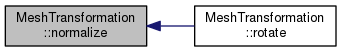
\includegraphics[width=328pt]{class_mesh_transformation_a62b90b65ce289707982efdb23a88e517_icgraph}
\end{center}
\end{figure}
\index{Mesh\+Transformation@{Mesh\+Transformation}!normalize@{normalize}}
\index{normalize@{normalize}!Mesh\+Transformation@{Mesh\+Transformation}}
\subsubsection[{\texorpdfstring{normalize(float3 axis) const}{normalize(float3 axis) const}}]{\setlength{\rightskip}{0pt plus 5cm}float3 Mesh\+Transformation\+::normalize (
\begin{DoxyParamCaption}
\item[{float3}]{axis}
\end{DoxyParamCaption}
) const\hspace{0.3cm}{\ttfamily [virtual]}}\hypertarget{class_mesh_transformation_a62b90b65ce289707982efdb23a88e517}{}\label{class_mesh_transformation_a62b90b65ce289707982efdb23a88e517}
Axis normalization. Required for rotation. 

Implements \hyperlink{class_pipeline}{Pipeline}.



The documentation for this class was generated from the following files\+:\begin{DoxyCompactItemize}
\item 
/home/god/cuda-\/workspace/r\+T\+Tracer/include/transformations.\+cuh\item 
/home/god/cuda-\/workspace/r\+T\+Tracer/source/transformations.\+cu\end{DoxyCompactItemize}

\hypertarget{class_object_box}{}\section{Object\+Box Class Reference}
\label{class_object_box}\index{Object\+Box@{Object\+Box}}


Collaboration diagram for Object\+Box\+:
\nopagebreak
\begin{figure}[H]
\begin{center}
\leavevmode
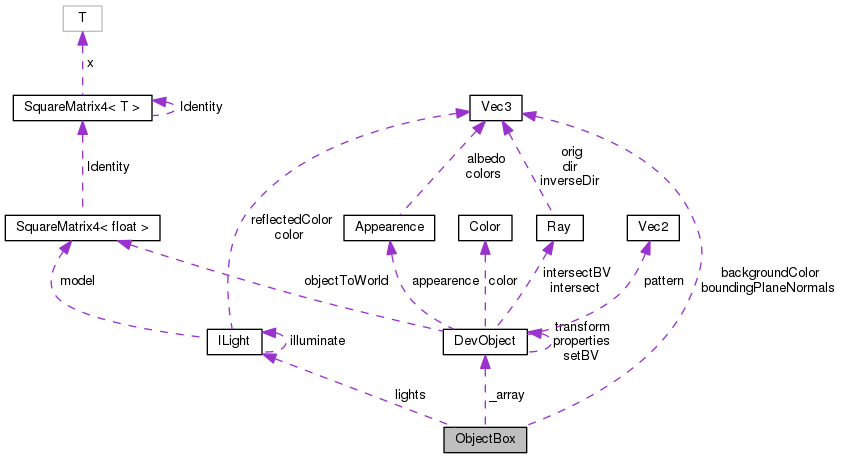
\includegraphics[width=350pt]{class_object_box__coll__graph}
\end{center}
\end{figure}
\subsection*{Public Member Functions}
\begin{DoxyCompactItemize}
\item 
{\bfseries Object\+Box} (std\+::vector$<$ \hyperlink{class_dev_object}{Dev\+Object} $>$ \&d\+Vec)\hypertarget{class_object_box_aafbc94494fbc8d4cdb62f8cb1f051003}{}\label{class_object_box_aafbc94494fbc8d4cdb62f8cb1f051003}

\item 
\+\_\+\+\_\+host\+\_\+\+\_\+ \+\_\+\+\_\+device\+\_\+\+\_\+ {\bfseries Object\+Box} (const \hyperlink{class_object_box}{Object\+Box} \&karr)\hypertarget{class_object_box_aa87628a92437a186a84efabb697a972f}{}\label{class_object_box_aa87628a92437a186a84efabb697a972f}

\item 
\+\_\+\+\_\+host\+\_\+\+\_\+ \+\_\+\+\_\+device\+\_\+\+\_\+ {\bfseries Object\+Box} (\hyperlink{class_dev_object}{Dev\+Object} $\ast$objects, int size)\hypertarget{class_object_box_af145281cc745ea12a7d323154d77a4a2}{}\label{class_object_box_af145281cc745ea12a7d323154d77a4a2}

\item 
\+\_\+\+\_\+host\+\_\+\+\_\+ \+\_\+\+\_\+device\+\_\+\+\_\+ \hyperlink{class_dev_object}{Dev\+Object} \& {\bfseries operator \mbox{[}$\,$\mbox{]}} (uint8\+\_\+t i)\hypertarget{class_object_box_a93aa063210479567f9817f8fe28db3f0}{}\label{class_object_box_a93aa063210479567f9817f8fe28db3f0}

\item 
\+\_\+\+\_\+device\+\_\+\+\_\+ bool {\bfseries hit} (\hyperlink{class_ray}{Ray} \&ray, Dev\+Priority\+Queue$<$ \hyperlink{class_dev_object}{Dev\+Object} $\ast$, M\+A\+X\+\_\+\+O\+B\+J\+E\+C\+TS $>$ \&queue, \hyperlink{struct_g_p_u_1_1_rendering_context}{G\+P\+U\+::\+Rendering\+Context} \&rctx)\hypertarget{class_object_box_a2414c6dfe6ea1f11fadbb37f96b9a463}{}\label{class_object_box_a2414c6dfe6ea1f11fadbb37f96b9a463}

\item 
\+\_\+\+\_\+host\+\_\+\+\_\+ \+\_\+\+\_\+device\+\_\+\+\_\+ \hyperlink{class_i_light}{I\+Light} \& {\bfseries getlight} (uint8\+\_\+t light\+Number)\hypertarget{class_object_box_adf08ee78e3a68ed05a02d3d2a677f04c}{}\label{class_object_box_adf08ee78e3a68ed05a02d3d2a677f04c}

\item 
void {\bfseries destroy} ()\hypertarget{class_object_box_ac5a98f92851297ed083ea54dd539d129}{}\label{class_object_box_ac5a98f92851297ed083ea54dd539d129}

\item 
\+\_\+\+\_\+host\+\_\+\+\_\+ \+\_\+\+\_\+device\+\_\+\+\_\+ \hyperlink{class_dev_object}{Dev\+Object} $\ast$ {\bfseries data} ()\hypertarget{class_object_box_ac5d2891a8048d7a80e4941c1235a5e9f}{}\label{class_object_box_ac5d2891a8048d7a80e4941c1235a5e9f}

\item 
{\bfseries Object\+Box} (std\+::vector$<$ \hyperlink{class_dev_object}{Dev\+Object} $>$ \&d\+Vec)\hypertarget{class_object_box_aafbc94494fbc8d4cdb62f8cb1f051003}{}\label{class_object_box_aafbc94494fbc8d4cdb62f8cb1f051003}

\item 
\+\_\+\+\_\+host\+\_\+\+\_\+ \+\_\+\+\_\+device\+\_\+\+\_\+ {\bfseries Object\+Box} (const \hyperlink{class_object_box}{Object\+Box} \&karr)\hypertarget{class_object_box_aa87628a92437a186a84efabb697a972f}{}\label{class_object_box_aa87628a92437a186a84efabb697a972f}

\item 
\+\_\+\+\_\+host\+\_\+\+\_\+ \+\_\+\+\_\+device\+\_\+\+\_\+ {\bfseries Object\+Box} (\hyperlink{class_dev_object}{Dev\+Object} $\ast$objects, int size)\hypertarget{class_object_box_af145281cc745ea12a7d323154d77a4a2}{}\label{class_object_box_af145281cc745ea12a7d323154d77a4a2}

\item 
\+\_\+\+\_\+host\+\_\+\+\_\+ \+\_\+\+\_\+device\+\_\+\+\_\+ \hyperlink{class_dev_object}{Dev\+Object} \& {\bfseries operator \mbox{[}$\,$\mbox{]}} (uint8\+\_\+t i)\hypertarget{class_object_box_aab4b56530190f6a452248e0a7547a76b}{}\label{class_object_box_aab4b56530190f6a452248e0a7547a76b}

\item 
\+\_\+\+\_\+device\+\_\+\+\_\+ bool {\bfseries hit} (\hyperlink{class_ray}{Ray} \&ray, Dev\+Priority\+Queue$<$ \hyperlink{class_dev_object}{Dev\+Object} $\ast$, M\+A\+X\+\_\+\+O\+B\+J\+E\+C\+TS $>$ \&queue, \hyperlink{struct_g_p_u_1_1_rendering_context}{G\+P\+U\+::\+Rendering\+Context} \&rctx)\hypertarget{class_object_box_a2414c6dfe6ea1f11fadbb37f96b9a463}{}\label{class_object_box_a2414c6dfe6ea1f11fadbb37f96b9a463}

\item 
\+\_\+\+\_\+host\+\_\+\+\_\+ \+\_\+\+\_\+device\+\_\+\+\_\+ \hyperlink{class_i_light}{I\+Light} \& {\bfseries getlight} (uint8\+\_\+t light\+Number)\hypertarget{class_object_box_a03450a7cc5c94af40e2416d72b0dfe69}{}\label{class_object_box_a03450a7cc5c94af40e2416d72b0dfe69}

\item 
void {\bfseries destroy} ()\hypertarget{class_object_box_ac5a98f92851297ed083ea54dd539d129}{}\label{class_object_box_ac5a98f92851297ed083ea54dd539d129}

\item 
\+\_\+\+\_\+host\+\_\+\+\_\+ \+\_\+\+\_\+device\+\_\+\+\_\+ \hyperlink{class_dev_object}{Dev\+Object} $\ast$ {\bfseries data} ()\hypertarget{class_object_box_a3838983908c17bea5c7659b464055f02}{}\label{class_object_box_a3838983908c17bea5c7659b464055f02}

\end{DoxyCompactItemize}
\subsection*{Public Attributes}
\begin{DoxyCompactItemize}
\item 
\hyperlink{class_dev_object}{Dev\+Object} $\ast$ {\bfseries \+\_\+array}\hypertarget{class_object_box_a1c5db29dce3ca086d225788ac6f5b1b9}{}\label{class_object_box_a1c5db29dce3ca086d225788ac6f5b1b9}

\item 
\hyperlink{class_i_light}{I\+Light} $\ast$ {\bfseries lights}\hypertarget{class_object_box_a4c242111384906aafc355ab98b148076}{}\label{class_object_box_a4c242111384906aafc355ab98b148076}

\item 
int {\bfseries \+\_\+size}\hypertarget{class_object_box_a5b8723c68c6d742bc04c601122612615}{}\label{class_object_box_a5b8723c68c6d742bc04c601122612615}

\item 
int {\bfseries lights\+Number}\hypertarget{class_object_box_add9c5ed5d73451037155bd85d53be522}{}\label{class_object_box_add9c5ed5d73451037155bd85d53be522}

\item 
\hyperlink{class_vec3}{Vec3f} {\bfseries bounding\+Plane\+Normals} \mbox{[}Boundaries\+::n\+Normals\mbox{]}\hypertarget{class_object_box_a082f8c59cead7723d2afd470b2376c6a}{}\label{class_object_box_a082f8c59cead7723d2afd470b2376c6a}

\item 
\hyperlink{class_vec3}{Vec3f} {\bfseries background\+Color}\hypertarget{class_object_box_a5e71a6c5ca56daf46ddf570730433f16}{}\label{class_object_box_a5e71a6c5ca56daf46ddf570730433f16}

\end{DoxyCompactItemize}


The documentation for this class was generated from the following files\+:\begin{DoxyCompactItemize}
\item 
/home/god/cuda-\/workspace/r\+T\+Tracer/include/object\+Box.\+cuh\item 
/home/god/cuda-\/workspace/r\+T\+Tracer/source/object\+Box.\+cu\end{DoxyCompactItemize}

\hypertarget{class_pipeline}{}\section{Pipeline Class Reference}
\label{class_pipeline}\index{Pipeline@{Pipeline}}


Interface  Convenient way to create and store a matrix transformation pipeline.~\newline
 a host-\/side implementation.~\newline
.  




Inheritance diagram for Pipeline\+:
\nopagebreak
\begin{figure}[H]
\begin{center}
\leavevmode
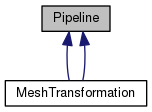
\includegraphics[width=186pt]{class_pipeline__inherit__graph}
\end{center}
\end{figure}
\subsection*{Public Member Functions}
\begin{DoxyCompactItemize}
\item 
virtual float3 {\bfseries normalize} (float3 axis) const =0\hypertarget{class_pipeline_a45a5dd1398482de5c9fd57ada431229d}{}\label{class_pipeline_a45a5dd1398482de5c9fd57ada431229d}

\item 
virtual \hyperlink{class_square_matrix4}{Square\+Matrix4f} {\bfseries transform} () const =0\hypertarget{class_pipeline_a8d5faa6d841fb9e6cc2527d904ad6bee}{}\label{class_pipeline_a8d5faa6d841fb9e6cc2527d904ad6bee}

\item 
virtual \hyperlink{class_square_matrix4}{Square\+Matrix4f} \& {\bfseries rotate} (const float3 \&axis, float deg\+Angle)=0\hypertarget{class_pipeline_a2b50d058b74ce266e58acd4ab1622ef9}{}\label{class_pipeline_a2b50d058b74ce266e58acd4ab1622ef9}

\item 
virtual \hyperlink{class_square_matrix4}{Square\+Matrix4f} \& {\bfseries translate} (float3 translation\+Point)=0\hypertarget{class_pipeline_a7c12b9fa044a6341e08d5639c9ee7db4}{}\label{class_pipeline_a7c12b9fa044a6341e08d5639c9ee7db4}

\item 
virtual \hyperlink{class_square_matrix4}{Square\+Matrix4f} \& {\bfseries scale} (float3 scale\+Factor)=0\hypertarget{class_pipeline_a60ed7a51148b346075ad5aa23c766d30}{}\label{class_pipeline_a60ed7a51148b346075ad5aa23c766d30}

\item 
virtual void {\bfseries reset} ()=0\hypertarget{class_pipeline_a632192d4703d48e1e7fec206c6dcddf7}{}\label{class_pipeline_a632192d4703d48e1e7fec206c6dcddf7}

\item 
virtual float3 {\bfseries normalize} (float3 axis) const =0\hypertarget{class_pipeline_a45a5dd1398482de5c9fd57ada431229d}{}\label{class_pipeline_a45a5dd1398482de5c9fd57ada431229d}

\item 
virtual \hyperlink{class_square_matrix4}{Square\+Matrix4f} {\bfseries transform} () const =0\hypertarget{class_pipeline_a8d5faa6d841fb9e6cc2527d904ad6bee}{}\label{class_pipeline_a8d5faa6d841fb9e6cc2527d904ad6bee}

\item 
virtual \hyperlink{class_square_matrix4}{Square\+Matrix4f} \& {\bfseries rotate} (const float3 \&axis, float deg\+Angle)=0\hypertarget{class_pipeline_a2b50d058b74ce266e58acd4ab1622ef9}{}\label{class_pipeline_a2b50d058b74ce266e58acd4ab1622ef9}

\item 
virtual \hyperlink{class_square_matrix4}{Square\+Matrix4f} \& {\bfseries translate} (float3 translation\+Point)=0\hypertarget{class_pipeline_a7c12b9fa044a6341e08d5639c9ee7db4}{}\label{class_pipeline_a7c12b9fa044a6341e08d5639c9ee7db4}

\item 
virtual \hyperlink{class_square_matrix4}{Square\+Matrix4f} \& {\bfseries scale} (float3 scale\+Factor)=0\hypertarget{class_pipeline_a60ed7a51148b346075ad5aa23c766d30}{}\label{class_pipeline_a60ed7a51148b346075ad5aa23c766d30}

\item 
virtual void {\bfseries reset} ()=0\hypertarget{class_pipeline_a632192d4703d48e1e7fec206c6dcddf7}{}\label{class_pipeline_a632192d4703d48e1e7fec206c6dcddf7}

\end{DoxyCompactItemize}


\subsection{Detailed Description}
Interface  Convenient way to create and store a matrix transformation pipeline.~\newline
 a host-\/side implementation.~\newline
. 

The documentation for this class was generated from the following file\+:\begin{DoxyCompactItemize}
\item 
/home/god/cuda-\/workspace/r\+T\+Tracer/include/transformations.\+cuh\end{DoxyCompactItemize}

\hypertarget{class_plane}{}\section{Plane Class Reference}
\label{class_plane}\index{Plane@{Plane}}


Inheritance diagram for Plane\+:
\nopagebreak
\begin{figure}[H]
\begin{center}
\leavevmode
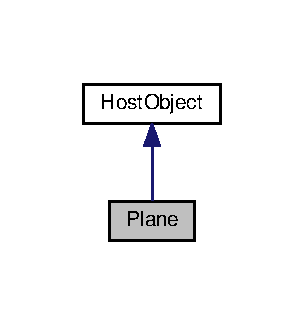
\includegraphics[width=146pt]{class_plane__inherit__graph}
\end{center}
\end{figure}


Collaboration diagram for Plane\+:
\nopagebreak
\begin{figure}[H]
\begin{center}
\leavevmode
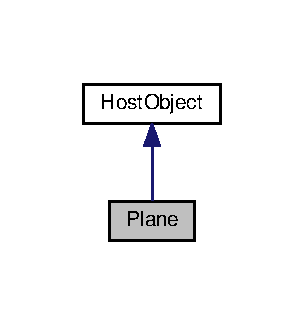
\includegraphics[width=146pt]{class_plane__coll__graph}
\end{center}
\end{figure}
\subsection*{Public Member Functions}
\begin{DoxyCompactItemize}
\item 
\+\_\+\+\_\+host\+\_\+\+\_\+ \+\_\+\+\_\+device\+\_\+\+\_\+ {\bfseries Plane} (const \hyperlink{class_plane}{Plane} \&plane)\hypertarget{class_plane_ad73917c92a73e36dcb1d716f79fdda04}{}\label{class_plane_ad73917c92a73e36dcb1d716f79fdda04}

\item 
\+\_\+\+\_\+host\+\_\+\+\_\+ \+\_\+\+\_\+device\+\_\+\+\_\+ {\bfseries Plane} (const \hyperlink{class_vec3}{Vec3f} \&first, const \hyperlink{class_vec3}{Vec3f} \&second, const \hyperlink{class_vec3}{Vec3f} \&third, const \hyperlink{class_vec3}{Vec3f} \&normal)\hypertarget{class_plane_adb0690a701aec7e890ffe616e05aa7b5}{}\label{class_plane_adb0690a701aec7e890ffe616e05aa7b5}

\item 
\+\_\+\+\_\+host\+\_\+\+\_\+ \+\_\+\+\_\+device\+\_\+\+\_\+ {\bfseries Plane} (const \hyperlink{class_vec3}{Vec3f} \&first, const \hyperlink{class_vec3}{Vec3f} \&second, const \hyperlink{class_vec3}{Vec3f} \&third)\hypertarget{class_plane_ab97bc9588363dbf0ed870ded0817d9b6}{}\label{class_plane_ab97bc9588363dbf0ed870ded0817d9b6}

\item 
\+\_\+\+\_\+host\+\_\+\+\_\+ \+\_\+\+\_\+device\+\_\+\+\_\+ const \hyperlink{class_vec3}{Vec3f} \& {\bfseries operator\mbox{[}$\,$\mbox{]}} (uint8\+\_\+t i) const\hypertarget{class_plane_ad0d581daf542b982afdfdbe7dc12d5f0}{}\label{class_plane_ad0d581daf542b982afdfdbe7dc12d5f0}

\item 
\+\_\+\+\_\+host\+\_\+\+\_\+ \+\_\+\+\_\+device\+\_\+\+\_\+ \hyperlink{class_vec3}{Vec3f} \& {\bfseries operator\mbox{[}$\,$\mbox{]}} (uint8\+\_\+t i)\hypertarget{class_plane_ae0980a97158717c8a0d543aecd8a0eca}{}\label{class_plane_ae0980a97158717c8a0d543aecd8a0eca}

\item 
\+\_\+\+\_\+host\+\_\+\+\_\+ \+\_\+\+\_\+device\+\_\+\+\_\+ \hyperlink{class_plane}{Plane} \& {\bfseries operator=} (const \hyperlink{class_plane}{Plane} \&plane)\hypertarget{class_plane_a028c720b343f768f876c531a67e64496}{}\label{class_plane_a028c720b343f768f876c531a67e64496}

\item 
\+\_\+\+\_\+host\+\_\+\+\_\+ \+\_\+\+\_\+device\+\_\+\+\_\+ const \hyperlink{class_vec3}{Vec3f} \& {\bfseries normal} () const\hypertarget{class_plane_a9132cbc2fc014812966ac919bb96f6bf}{}\label{class_plane_a9132cbc2fc014812966ac919bb96f6bf}

\item 
\+\_\+\+\_\+host\+\_\+\+\_\+ \+\_\+\+\_\+device\+\_\+\+\_\+ const float \& {\bfseries width} () const\hypertarget{class_plane_a1c91bd58a15624b97a10912ed8169406}{}\label{class_plane_a1c91bd58a15624b97a10912ed8169406}

\item 
\+\_\+\+\_\+host\+\_\+\+\_\+ \+\_\+\+\_\+device\+\_\+\+\_\+ const float \& {\bfseries height} () const\hypertarget{class_plane_af8ebbcfced6954ead0f5efc91c532b95}{}\label{class_plane_af8ebbcfced6954ead0f5efc91c532b95}

\item 
\+\_\+\+\_\+host\+\_\+\+\_\+ \+\_\+\+\_\+device\+\_\+\+\_\+ void {\bfseries swap} (\hyperlink{class_plane}{Plane} \&plane)\hypertarget{class_plane_abd61cd7527ed084a867050bee3f4c4ec}{}\label{class_plane_abd61cd7527ed084a867050bee3f4c4ec}

\item 
\hyperlink{struct_polymorphic}{Polymorphic} {\bfseries get\+Device\+Polymorphic} (const Pattern \&dev\+\_\+pattern) const\hypertarget{class_plane_a67ce79f9411d96c278f0a3e7c2438f11}{}\label{class_plane_a67ce79f9411d96c278f0a3e7c2438f11}

\item 
void $\ast$ {\bfseries get\+Object} ()\hypertarget{class_plane_ac638c29a88ee505c9b84bcf79ba67509}{}\label{class_plane_ac638c29a88ee505c9b84bcf79ba67509}

\item 
size\+\_\+t {\bfseries bytes} () const\hypertarget{class_plane_a8a95c1d089d188c4c927bc67e5139775}{}\label{class_plane_a8a95c1d089d188c4c927bc67e5139775}

\item 
size\+\_\+t {\bfseries get\+Verts\+Number} () const\hypertarget{class_plane_aecf40d0480c922b6513be086f1a732a7}{}\label{class_plane_aecf40d0480c922b6513be086f1a732a7}

\end{DoxyCompactItemize}
\subsection*{Static Public Attributes}
\begin{DoxyCompactItemize}
\item 
static const size\+\_\+t {\bfseries verts\+Number} = 4\hypertarget{class_plane_a6b7d31dd30df60bfde03401356211b96}{}\label{class_plane_a6b7d31dd30df60bfde03401356211b96}

\end{DoxyCompactItemize}


The documentation for this class was generated from the following files\+:\begin{DoxyCompactItemize}
\item 
/home/god/cuda-\/workspace/r\+T\+Tracer/include/object\+Box.\+cuh\item 
/home/god/cuda-\/workspace/r\+T\+Tracer/include/geometry\+Loader.\+cuh\item 
/home/god/cuda-\/workspace/r\+T\+Tracer/source/object\+Box.\+cu\end{DoxyCompactItemize}

\hypertarget{class_point_light}{}\section{Point\+Light$<$ Point\+Type $>$ Class Template Reference}
\label{class_point_light}\index{Point\+Light$<$ Point\+Type $>$@{Point\+Light$<$ Point\+Type $>$}}


requires distance, unaffected by rotation  


\subsection*{Public Member Functions}
\begin{DoxyCompactItemize}
\item 
\+\_\+\+\_\+host\+\_\+\+\_\+ \+\_\+\+\_\+device\+\_\+\+\_\+ {\bfseries Point\+Light} (const \hyperlink{class_square_matrix4}{Square\+Matrix4f} \&model)\hypertarget{class_point_light_a01fae78fac3286f01acead5ad0dadf8b}{}\label{class_point_light_a01fae78fac3286f01acead5ad0dadf8b}

\item 
\+\_\+\+\_\+host\+\_\+\+\_\+ \+\_\+\+\_\+device\+\_\+\+\_\+ {\bfseries Point\+Light} (const \hyperlink{class_square_matrix4}{Square\+Matrix4f} \&model)\hypertarget{class_point_light_a01fae78fac3286f01acead5ad0dadf8b}{}\label{class_point_light_a01fae78fac3286f01acead5ad0dadf8b}

\end{DoxyCompactItemize}
\subsection*{Public Attributes}
\begin{DoxyCompactItemize}
\item 
Point\+Type {\bfseries pos}\hypertarget{class_point_light_a5546247e7a8ccc1ff713898703f1db07}{}\label{class_point_light_a5546247e7a8ccc1ff713898703f1db07}

\end{DoxyCompactItemize}


\subsection{Detailed Description}
\subsubsection*{template$<$typename Point\+Type$>$\\*
class Point\+Light$<$ Point\+Type $>$}

requires distance, unaffected by rotation 

Spherical light 

The documentation for this class was generated from the following file\+:\begin{DoxyCompactItemize}
\item 
/home/god/cuda-\/workspace/r\+T\+Tracer/include/light.\+cuh\end{DoxyCompactItemize}

\hypertarget{struct_polymorphic}{}\section{Polymorphic Struct Reference}
\label{struct_polymorphic}\index{Polymorphic@{Polymorphic}}
\subsection*{Public Member Functions}
\begin{DoxyCompactItemize}
\item 
\hyperlink{struct_polymorphic_a8a1a7aa3ea005bcf84bd8110d9b6a9f2}{Polymorphic} (const Intersect \&\hyperlink{group__device__pointers_ga00654ffb007d4b5c95c00b429dc26ae9}{dev\+\_\+intersect}=nullptr, const Properties \&\hyperlink{group__device__pointers_gac0d627981d2453b8f45dc3cca7a69a28}{dev\+\_\+properties}=nullptr, const Intersect\+BV \&\hyperlink{group__device__pointers_gaeee39cf2f67c91f2a6c312651283dc94}{dev\+\_\+intersect\+BV}=nullptr, const Transform \&\hyperlink{group__device__pointers_gac3760d5ca4da6826e005200738140558}{dev\+\_\+transform}=nullptr, const Set\+BV \&set\+BV=nullptr, const Pattern \&dev\+\_\+pattern=nullptr)
\end{DoxyCompactItemize}
\subsection*{Public Attributes}
\begin{DoxyCompactItemize}
\item 
const Intersect \& {\bfseries intersect}\hypertarget{struct_polymorphic_a5f3c42ecfadb152a3658a00c0ecb1873}{}\label{struct_polymorphic_a5f3c42ecfadb152a3658a00c0ecb1873}

\item 
const Properties \& {\bfseries properties}\hypertarget{struct_polymorphic_aee39f2f94f8cbbb7d82a5c89bc879023}{}\label{struct_polymorphic_aee39f2f94f8cbbb7d82a5c89bc879023}

\item 
const Intersect\+BV \& {\bfseries intersect\+BV}\hypertarget{struct_polymorphic_afe3626a4aa28bfc95bfae27e624f86f6}{}\label{struct_polymorphic_afe3626a4aa28bfc95bfae27e624f86f6}

\item 
const Transform \& {\bfseries transform}\hypertarget{struct_polymorphic_ad748762337dae443f098dd531e7781d2}{}\label{struct_polymorphic_ad748762337dae443f098dd531e7781d2}

\item 
const Set\+BV \& {\bfseries set\+BV}\hypertarget{struct_polymorphic_aa71af495247c0c740b66ab32c242505a}{}\label{struct_polymorphic_aa71af495247c0c740b66ab32c242505a}

\item 
const Pattern \& {\bfseries pattern}\hypertarget{struct_polymorphic_a9dc360effd8472a7c174993e6a02dfbf}{}\label{struct_polymorphic_a9dc360effd8472a7c174993e6a02dfbf}

\end{DoxyCompactItemize}


\subsection{Constructor \& Destructor Documentation}
\index{Polymorphic@{Polymorphic}!Polymorphic@{Polymorphic}}
\index{Polymorphic@{Polymorphic}!Polymorphic@{Polymorphic}}
\subsubsection[{\texorpdfstring{Polymorphic(const Intersect \&dev\+\_\+intersect=nullptr, const Properties \&dev\+\_\+properties=nullptr, const Intersect\+B\+V \&dev\+\_\+intersect\+B\+V=nullptr, const Transform \&dev\+\_\+transform=nullptr, const Set\+B\+V \&set\+B\+V=nullptr, const Pattern \&dev\+\_\+pattern=nullptr)}{Polymorphic(const Intersect \&dev\_intersect=nullptr, const Properties \&dev\_properties=nullptr, const IntersectBV \&dev\_intersectBV=nullptr, const Transform \&dev\_transform=nullptr, const SetBV \&setBV=nullptr, const Pattern \&dev\_pattern=nullptr)}}]{\setlength{\rightskip}{0pt plus 5cm}Polymorphic\+::\+Polymorphic (
\begin{DoxyParamCaption}
\item[{const Intersect \&}]{dev\+\_\+intersect = {\ttfamily nullptr}, }
\item[{const Properties \&}]{dev\+\_\+properties = {\ttfamily nullptr}, }
\item[{const Intersect\+BV \&}]{dev\+\_\+intersect\+BV = {\ttfamily nullptr}, }
\item[{const Transform \&}]{dev\+\_\+transform = {\ttfamily nullptr}, }
\item[{const Set\+BV \&}]{set\+BV = {\ttfamily nullptr}, }
\item[{const Pattern \&}]{dev\+\_\+pattern = {\ttfamily nullptr}}
\end{DoxyParamCaption}
)\hspace{0.3cm}{\ttfamily [inline]}}\hypertarget{struct_polymorphic_a8a1a7aa3ea005bcf84bd8110d9b6a9f2}{}\label{struct_polymorphic_a8a1a7aa3ea005bcf84bd8110d9b6a9f2}

\begin{DoxyParams}[1]{Parameters}
\mbox{\tt in}  & {\em dev\+\_\+intersect} & -\/ pointer to the intersection test function \\
\hline
\mbox{\tt in}  & {\em dev\+\_\+properties} & -\/ pointer to the function which gets normal, texture coordinates, etc. \\
\hline
\mbox{\tt in}  & {\em dev\+\_\+intersect\+BV} & -\/ bounding volume intersect test function pointer \\
\hline
\mbox{\tt in}  & {\em dev\+\_\+transform} & -\/ pointer to the object transformation function \\
\hline
\mbox{\tt in}  & {\em set\+BV} & -\/ pointer to the bounding volume set up function \\
\hline
\mbox{\tt in}  & {\em dev\+\_\+pattern} & -\/ pointer to the texturing function \\
\hline
\end{DoxyParams}


The documentation for this struct was generated from the following file\+:\begin{DoxyCompactItemize}
\item 
/home/god/cuda-\/workspace/r\+T\+Tracer/include/object\+Box.\+cuh\end{DoxyCompactItemize}

\hypertarget{class_quaternion}{}\section{Quaternion Class Reference}
\label{class_quaternion}\index{Quaternion@{Quaternion}}
\subsection*{Public Member Functions}
\begin{DoxyCompactItemize}
\item 
\+\_\+\+\_\+host\+\_\+\+\_\+ \+\_\+\+\_\+device\+\_\+\+\_\+ {\bfseries Quaternion} (float x, float y, float z, float w)\hypertarget{class_quaternion_a1a4bd86f9d61fd86784c4c0242706f71}{}\label{class_quaternion_a1a4bd86f9d61fd86784c4c0242706f71}

\item 
\+\_\+\+\_\+host\+\_\+\+\_\+ \+\_\+\+\_\+device\+\_\+\+\_\+ float {\bfseries length} ()\hypertarget{class_quaternion_a78a3e8c21812d2311790df5152e3c139}{}\label{class_quaternion_a78a3e8c21812d2311790df5152e3c139}

\item 
\+\_\+\+\_\+host\+\_\+\+\_\+ \+\_\+\+\_\+device\+\_\+\+\_\+ \hyperlink{class_quaternion}{Quaternion} {\bfseries Normalize} ()\hypertarget{class_quaternion_a90a71b875a7bc6e705e829805e748184}{}\label{class_quaternion_a90a71b875a7bc6e705e829805e748184}

\item 
\+\_\+\+\_\+host\+\_\+\+\_\+ \+\_\+\+\_\+device\+\_\+\+\_\+ \hyperlink{class_square_matrix4}{Square\+Matrix4f} {\bfseries to\+Matrix} ()\hypertarget{class_quaternion_a5474d0118b84350ddbd163bdd7ff1e60}{}\label{class_quaternion_a5474d0118b84350ddbd163bdd7ff1e60}

\item 
\+\_\+\+\_\+host\+\_\+\+\_\+ \+\_\+\+\_\+device\+\_\+\+\_\+ \hyperlink{class_quaternion}{Quaternion} \hyperlink{class_quaternion_aee895e4a7d8f3d0e8a65d9ddea5b24b5}{conjugate} ()
\item 
\+\_\+\+\_\+host\+\_\+\+\_\+ \+\_\+\+\_\+device\+\_\+\+\_\+ {\bfseries Quaternion} (float x, float y, float z, float w)\hypertarget{class_quaternion_a1a4bd86f9d61fd86784c4c0242706f71}{}\label{class_quaternion_a1a4bd86f9d61fd86784c4c0242706f71}

\item 
\+\_\+\+\_\+host\+\_\+\+\_\+ \+\_\+\+\_\+device\+\_\+\+\_\+ float {\bfseries length} ()\hypertarget{class_quaternion_a78a3e8c21812d2311790df5152e3c139}{}\label{class_quaternion_a78a3e8c21812d2311790df5152e3c139}

\item 
\+\_\+\+\_\+host\+\_\+\+\_\+ \+\_\+\+\_\+device\+\_\+\+\_\+ \hyperlink{class_quaternion}{Quaternion} {\bfseries Normalize} ()\hypertarget{class_quaternion_a90a71b875a7bc6e705e829805e748184}{}\label{class_quaternion_a90a71b875a7bc6e705e829805e748184}

\item 
\+\_\+\+\_\+host\+\_\+\+\_\+ \+\_\+\+\_\+device\+\_\+\+\_\+ \hyperlink{class_square_matrix4}{Square\+Matrix4f} {\bfseries to\+Matrix} ()\hypertarget{class_quaternion_a5474d0118b84350ddbd163bdd7ff1e60}{}\label{class_quaternion_a5474d0118b84350ddbd163bdd7ff1e60}

\item 
\+\_\+\+\_\+host\+\_\+\+\_\+ \+\_\+\+\_\+device\+\_\+\+\_\+ \hyperlink{class_quaternion}{Quaternion} \hyperlink{class_quaternion_aee895e4a7d8f3d0e8a65d9ddea5b24b5}{conjugate} ()
\end{DoxyCompactItemize}
\subsection*{Public Attributes}
\begin{DoxyCompactItemize}
\item 
float4 {\bfseries xyzw}\hypertarget{class_quaternion_aaa1be23ee999c4dd0a7c670db2dbf10c}{}\label{class_quaternion_aaa1be23ee999c4dd0a7c670db2dbf10c}

\end{DoxyCompactItemize}


\subsection{Member Function Documentation}
\index{Quaternion@{Quaternion}!conjugate@{conjugate}}
\index{conjugate@{conjugate}!Quaternion@{Quaternion}}
\subsubsection[{\texorpdfstring{conjugate()}{conjugate()}}]{\setlength{\rightskip}{0pt plus 5cm}\+\_\+\+\_\+host\+\_\+\+\_\+ \+\_\+\+\_\+device\+\_\+\+\_\+ {\bf Quaternion} Quaternion\+::conjugate (
\begin{DoxyParamCaption}
{}
\end{DoxyParamCaption}
)}\hypertarget{class_quaternion_aee895e4a7d8f3d0e8a65d9ddea5b24b5}{}\label{class_quaternion_aee895e4a7d8f3d0e8a65d9ddea5b24b5}
$ Q = (V, w)$ or $ Q = (sin(a/2), U*sin(a/2) ) $, to inverse we should get $sin$ negative because $cos$ will not has any effect either $V$ or $w$ should be negative to inverse rotation \index{Quaternion@{Quaternion}!conjugate@{conjugate}}
\index{conjugate@{conjugate}!Quaternion@{Quaternion}}
\subsubsection[{\texorpdfstring{conjugate()}{conjugate()}}]{\setlength{\rightskip}{0pt plus 5cm}\+\_\+\+\_\+host\+\_\+\+\_\+ \+\_\+\+\_\+device\+\_\+\+\_\+ {\bf Quaternion} Quaternion\+::conjugate (
\begin{DoxyParamCaption}
{}
\end{DoxyParamCaption}
)}\hypertarget{class_quaternion_aee895e4a7d8f3d0e8a65d9ddea5b24b5}{}\label{class_quaternion_aee895e4a7d8f3d0e8a65d9ddea5b24b5}
$ Q = (V, w)$ or $ Q = (sin(a/2), U*sin(a/2) ) $, to inverse we should get $sin$ negative because $cos$ will not has any effect either $V$ or $w$ should be negative to inverse rotation 

The documentation for this class was generated from the following files\+:\begin{DoxyCompactItemize}
\item 
/home/god/cuda-\/workspace/r\+T\+Tracer/include/\hyperlink{r_t_tracer_2include_2geom_8cuh}{geom.\+cuh}\item 
/home/god/cuda-\/workspace/r\+T\+Tracer/source/geom.\+cu\end{DoxyCompactItemize}

\hypertarget{class_ray}{}\section{Ray Class Reference}
\label{class_ray}\index{Ray@{Ray}}


Collaboration diagram for Ray\+:
\nopagebreak
\begin{figure}[H]
\begin{center}
\leavevmode
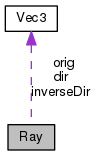
\includegraphics[width=145pt]{class_ray__coll__graph}
\end{center}
\end{figure}
\subsection*{Public Member Functions}
\begin{DoxyCompactItemize}
\item 
\+\_\+\+\_\+host\+\_\+\+\_\+ \+\_\+\+\_\+device\+\_\+\+\_\+ {\bfseries Ray} (const \hyperlink{class_vec3}{Vec3f} \&o, const \hyperlink{class_vec3}{Vec3f} \&d, const Ray\+Type \&ray\+Type=P\+R\+I\+M\+A\+R\+Y\+\_\+\+R\+AY)\hypertarget{class_ray_a70dc24e77fd2f372f64481b84352ea79}{}\label{class_ray_a70dc24e77fd2f372f64481b84352ea79}

\item 
\+\_\+\+\_\+host\+\_\+\+\_\+ \+\_\+\+\_\+device\+\_\+\+\_\+ {\bfseries Ray} (const \hyperlink{class_ray}{Ray} \&ray)\hypertarget{class_ray_a6d8a9d6b5b86ab607f5713a88943095c}{}\label{class_ray_a6d8a9d6b5b86ab607f5713a88943095c}

\item 
\+\_\+\+\_\+host\+\_\+\+\_\+ \+\_\+\+\_\+device\+\_\+\+\_\+ \hyperlink{class_ray}{Ray} \& {\bfseries operator=} (const \hyperlink{class_ray}{Ray} \&ray)\hypertarget{class_ray_ae5f0c2eebb56ef7f3e4d43a49bfc94a7}{}\label{class_ray_ae5f0c2eebb56ef7f3e4d43a49bfc94a7}

\item 
\+\_\+\+\_\+host\+\_\+\+\_\+ \+\_\+\+\_\+device\+\_\+\+\_\+ void {\bfseries swap} (\hyperlink{class_ray}{Ray} \&ray)\hypertarget{class_ray_ac55e80131f5422dd969190ebb56a4be7}{}\label{class_ray_ac55e80131f5422dd969190ebb56a4be7}

\item 
\+\_\+\+\_\+host\+\_\+\+\_\+ \+\_\+\+\_\+device\+\_\+\+\_\+ float4 {\bfseries direction} ()\hypertarget{class_ray_afa09f7613e0f5e5e7e0d1093ea83df6b}{}\label{class_ray_afa09f7613e0f5e5e7e0d1093ea83df6b}

\end{DoxyCompactItemize}
\subsection*{Public Attributes}
\begin{DoxyCompactItemize}
\item 
\hyperlink{class_vec3}{Vec3f} {\bfseries orig}\hypertarget{class_ray_a83060ce4752b7178322491c3ba060aeb}{}\label{class_ray_a83060ce4752b7178322491c3ba060aeb}

\item 
\hyperlink{class_vec3}{Vec3f} {\bfseries dir}\hypertarget{class_ray_abb6aec8e6d0ce79e31ccaf7cc0bd2f5e}{}\label{class_ray_abb6aec8e6d0ce79e31ccaf7cc0bd2f5e}

\item 
\hyperlink{class_vec3}{Vec3f} {\bfseries inverse\+Dir}\hypertarget{class_ray_a4aeb023e811e12834cb8e1daaf1e3db4}{}\label{class_ray_a4aeb023e811e12834cb8e1daaf1e3db4}

\item 
float {\bfseries t\+Min}\hypertarget{class_ray_a79bb8e0202bc33a3035b59b0cc25716d}{}\label{class_ray_a79bb8e0202bc33a3035b59b0cc25716d}

\item 
float {\bfseries t\+Max}\hypertarget{class_ray_a02e897e4b9c32cf86b7a28b44655b991}{}\label{class_ray_a02e897e4b9c32cf86b7a28b44655b991}

\item 
float {\bfseries t}\hypertarget{class_ray_a4ec5a9098b620bda59d15b0a4f99d454}{}\label{class_ray_a4ec5a9098b620bda59d15b0a4f99d454}

\item 
float {\bfseries t\+Nearest}\hypertarget{class_ray_ac729496eee350d328c4bff50b8235baf}{}\label{class_ray_ac729496eee350d328c4bff50b8235baf}

\item 
Ray\+Type {\bfseries ray\+Type}\hypertarget{class_ray_a53798941244349eeb1b61d9a3cef8425}{}\label{class_ray_a53798941244349eeb1b61d9a3cef8425}

\end{DoxyCompactItemize}


The documentation for this class was generated from the following file\+:\begin{DoxyCompactItemize}
\item 
/home/god/cuda-\/workspace/r\+T\+Tracer/include/\hyperlink{geom_8cuh}{geom.\+cuh}\end{DoxyCompactItemize}

\hypertarget{struct_g_p_u_1_1_rendering_context}{}\section{G\+PU\+:\+:Rendering\+Context Struct Reference}
\label{struct_g_p_u_1_1_rendering_context}\index{G\+P\+U\+::\+Rendering\+Context@{G\+P\+U\+::\+Rendering\+Context}}


Collaboration diagram for G\+PU\+:\+:Rendering\+Context\+:
\nopagebreak
\begin{figure}[H]
\begin{center}
\leavevmode
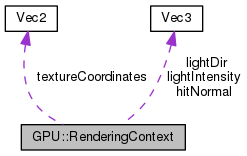
\includegraphics[width=258pt]{struct_g_p_u_1_1_rendering_context__coll__graph}
\end{center}
\end{figure}
\subsection*{Public Member Functions}
\begin{DoxyCompactItemize}
\item 
\+\_\+\+\_\+host\+\_\+\+\_\+ \+\_\+\+\_\+device\+\_\+\+\_\+ {\bfseries Rendering\+Context} (const \hyperlink{struct_g_p_u_1_1_rendering_context}{Rendering\+Context} \&rctx)\hypertarget{struct_g_p_u_1_1_rendering_context_afe4884d3990468289b68d97f3374de53}{}\label{struct_g_p_u_1_1_rendering_context_afe4884d3990468289b68d97f3374de53}

\item 
\+\_\+\+\_\+host\+\_\+\+\_\+ \+\_\+\+\_\+device\+\_\+\+\_\+ \hyperlink{struct_g_p_u_1_1_rendering_context}{Rendering\+Context} \& {\bfseries operator=} (const \hyperlink{struct_g_p_u_1_1_rendering_context}{Rendering\+Context} \&rctx)\hypertarget{struct_g_p_u_1_1_rendering_context_a9e187b5378b9ef7f95870a16be6c42d5}{}\label{struct_g_p_u_1_1_rendering_context_a9e187b5378b9ef7f95870a16be6c42d5}

\item 
\+\_\+\+\_\+host\+\_\+\+\_\+ \+\_\+\+\_\+device\+\_\+\+\_\+ void {\bfseries swap} (\hyperlink{struct_g_p_u_1_1_rendering_context}{Rendering\+Context} \&rctx)\hypertarget{struct_g_p_u_1_1_rendering_context_a03ef8006865af61b7010de8f4a76a3a3}{}\label{struct_g_p_u_1_1_rendering_context_a03ef8006865af61b7010de8f4a76a3a3}

\item 
\+\_\+\+\_\+host\+\_\+\+\_\+ \+\_\+\+\_\+device\+\_\+\+\_\+ {\bfseries Rendering\+Context} (const \hyperlink{struct_g_p_u_1_1_rendering_context}{Rendering\+Context} \&rctx)\hypertarget{struct_g_p_u_1_1_rendering_context_afe4884d3990468289b68d97f3374de53}{}\label{struct_g_p_u_1_1_rendering_context_afe4884d3990468289b68d97f3374de53}

\item 
\+\_\+\+\_\+host\+\_\+\+\_\+ \+\_\+\+\_\+device\+\_\+\+\_\+ \hyperlink{struct_g_p_u_1_1_rendering_context}{Rendering\+Context} \& {\bfseries operator=} (const \hyperlink{struct_g_p_u_1_1_rendering_context}{Rendering\+Context} \&rctx)\hypertarget{struct_g_p_u_1_1_rendering_context_a9e187b5378b9ef7f95870a16be6c42d5}{}\label{struct_g_p_u_1_1_rendering_context_a9e187b5378b9ef7f95870a16be6c42d5}

\item 
\+\_\+\+\_\+host\+\_\+\+\_\+ \+\_\+\+\_\+device\+\_\+\+\_\+ void {\bfseries swap} (\hyperlink{struct_g_p_u_1_1_rendering_context}{Rendering\+Context} \&rctx)\hypertarget{struct_g_p_u_1_1_rendering_context_a03ef8006865af61b7010de8f4a76a3a3}{}\label{struct_g_p_u_1_1_rendering_context_a03ef8006865af61b7010de8f4a76a3a3}

\end{DoxyCompactItemize}
\subsection*{Public Attributes}
\begin{DoxyCompactItemize}
\item 
uint32\+\_\+t {\bfseries triangle\+Index}\hypertarget{struct_g_p_u_1_1_rendering_context_a3f3cbd7668f1e3284e6d81a6ff45af15}{}\label{struct_g_p_u_1_1_rendering_context_a3f3cbd7668f1e3284e6d81a6ff45af15}

\item 
\hyperlink{class_vec2}{Vec2f} {\bfseries texture\+Coordinates}\hypertarget{struct_g_p_u_1_1_rendering_context_adb0db7d6cac7e75aac9022bc1a6e5d4c}{}\label{struct_g_p_u_1_1_rendering_context_adb0db7d6cac7e75aac9022bc1a6e5d4c}

\item 
\hyperlink{class_vec3}{Vec3f} {\bfseries hit\+Normal}\hypertarget{struct_g_p_u_1_1_rendering_context_ab52a46edf31d08fbb3e38b7e4973440e}{}\label{struct_g_p_u_1_1_rendering_context_ab52a46edf31d08fbb3e38b7e4973440e}

\item 
int {\bfseries index}\hypertarget{struct_g_p_u_1_1_rendering_context_aac9e3cc37208b4379d493b2ba669e33c}{}\label{struct_g_p_u_1_1_rendering_context_aac9e3cc37208b4379d493b2ba669e33c}

\item 
const float {\bfseries bias} = 0.\+001f\hypertarget{struct_g_p_u_1_1_rendering_context_a942e8aeb662e5b24f782c38fb172d99e}{}\label{struct_g_p_u_1_1_rendering_context_a942e8aeb662e5b24f782c38fb172d99e}

\item 
\hyperlink{class_vec3}{Vec3f} {\bfseries light\+Dir}\hypertarget{struct_g_p_u_1_1_rendering_context_a205c2dfe9842e0aea733e4bbb1da4e52}{}\label{struct_g_p_u_1_1_rendering_context_a205c2dfe9842e0aea733e4bbb1da4e52}

\item 
\hyperlink{class_vec3}{Vec3f} {\bfseries light\+Intensity}\hypertarget{struct_g_p_u_1_1_rendering_context_aa05e2be366dd8c157851ce8cbe00ed56}{}\label{struct_g_p_u_1_1_rendering_context_aa05e2be366dd8c157851ce8cbe00ed56}

\item 
const float {\bfseries max\+Depth} = 5\hypertarget{struct_g_p_u_1_1_rendering_context_a4b82358bf664122a391de3ff07519829}{}\label{struct_g_p_u_1_1_rendering_context_a4b82358bf664122a391de3ff07519829}

\end{DoxyCompactItemize}


The documentation for this struct was generated from the following file\+:\begin{DoxyCompactItemize}
\item 
/home/god/cuda-\/workspace/r\+T\+Tracer/include/\hyperlink{r_t_tracer_2include_2geom_8cuh}{geom.\+cuh}\end{DoxyCompactItemize}

\hypertarget{class_sphere}{}\section{Sphere Class Reference}
\label{class_sphere}\index{Sphere@{Sphere}}


Inheritance diagram for Sphere\+:
\nopagebreak
\begin{figure}[H]
\begin{center}
\leavevmode
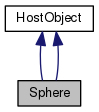
\includegraphics[width=146pt]{class_sphere__inherit__graph}
\end{center}
\end{figure}


Collaboration diagram for Sphere\+:
\nopagebreak
\begin{figure}[H]
\begin{center}
\leavevmode
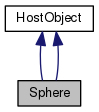
\includegraphics[width=146pt]{class_sphere__coll__graph}
\end{center}
\end{figure}
\subsection*{Public Member Functions}
\begin{DoxyCompactItemize}
\item 
\+\_\+\+\_\+host\+\_\+\+\_\+ \+\_\+\+\_\+device\+\_\+\+\_\+ {\bfseries Sphere} (const \hyperlink{class_square_matrix4}{Square\+Matrix4f} \&model, const float \&radius, \hyperlink{class_vec3}{Vec3f}(\&plane\+Normal)\mbox{[}N\+O\+R\+M\+A\+LS\mbox{]})\hypertarget{class_sphere_a6202639ed0ffaf44a7eaa55953eae1f9}{}\label{class_sphere_a6202639ed0ffaf44a7eaa55953eae1f9}

\item 
\+\_\+\+\_\+host\+\_\+\+\_\+ \+\_\+\+\_\+device\+\_\+\+\_\+ {\bfseries Sphere} (const \hyperlink{class_vec3}{Vec3f} \&center, const float \&radius, \hyperlink{class_vec3}{Vec3f}(\&plane\+Normal)\mbox{[}N\+O\+R\+M\+A\+LS\mbox{]})\hypertarget{class_sphere_afb7e10efe86404fc6df407381cc8fdcd}{}\label{class_sphere_afb7e10efe86404fc6df407381cc8fdcd}

\item 
\+\_\+\+\_\+host\+\_\+\+\_\+ \+\_\+\+\_\+device\+\_\+\+\_\+ {\bfseries Sphere} (const \hyperlink{class_sphere}{Sphere} \&sphere)\hypertarget{class_sphere_af805e2d486b9a5be47852afc1636e509}{}\label{class_sphere_af805e2d486b9a5be47852afc1636e509}

\item 
\+\_\+\+\_\+host\+\_\+\+\_\+ \+\_\+\+\_\+device\+\_\+\+\_\+ const float \& {\bfseries operator\mbox{[}$\,$\mbox{]}} (uint8\+\_\+t i) const\hypertarget{class_sphere_a4e0c5c168574e71ce6126a22d64c2ce7}{}\label{class_sphere_a4e0c5c168574e71ce6126a22d64c2ce7}

\item 
\+\_\+\+\_\+host\+\_\+\+\_\+ \+\_\+\+\_\+device\+\_\+\+\_\+ float \& {\bfseries operator\mbox{[}$\,$\mbox{]}} (uint8\+\_\+t i)\hypertarget{class_sphere_adb1f756dd4a5865993d055bd27b96d07}{}\label{class_sphere_adb1f756dd4a5865993d055bd27b96d07}

\item 
\+\_\+\+\_\+host\+\_\+\+\_\+ \+\_\+\+\_\+device\+\_\+\+\_\+ float {\bfseries radius} () const\hypertarget{class_sphere_a90c900da43ea7b40e7c7e0fd66fbf8f2}{}\label{class_sphere_a90c900da43ea7b40e7c7e0fd66fbf8f2}

\item 
\+\_\+\+\_\+host\+\_\+\+\_\+ \+\_\+\+\_\+device\+\_\+\+\_\+ float {\bfseries square\+Radius} () const\hypertarget{class_sphere_a00919fefbe3c39b8b749296fbfd3d856}{}\label{class_sphere_a00919fefbe3c39b8b749296fbfd3d856}

\item 
\+\_\+\+\_\+host\+\_\+\+\_\+ \+\_\+\+\_\+device\+\_\+\+\_\+ const \hyperlink{class_vec3}{Vec3f} \& {\bfseries center} () const\hypertarget{class_sphere_aa42da7338d536728abf563bc57fcb819}{}\label{class_sphere_aa42da7338d536728abf563bc57fcb819}

\item 
\+\_\+\+\_\+host\+\_\+\+\_\+ \+\_\+\+\_\+device\+\_\+\+\_\+ \hyperlink{class_vec3}{Vec3f} \& {\bfseries center} ()\hypertarget{class_sphere_a15a8c4847cea8d3a72ea91f9c71e8160}{}\label{class_sphere_a15a8c4847cea8d3a72ea91f9c71e8160}

\item 
\+\_\+\+\_\+host\+\_\+\+\_\+ \+\_\+\+\_\+device\+\_\+\+\_\+ void {\bfseries print\+Points} (int number) const\hypertarget{class_sphere_a80b41ffe0cbe37bc7a174e2e2c3cd12d}{}\label{class_sphere_a80b41ffe0cbe37bc7a174e2e2c3cd12d}

\item 
\+\_\+\+\_\+host\+\_\+\+\_\+ \+\_\+\+\_\+device\+\_\+\+\_\+ void {\bfseries plane\+Tangent\+Point} (\hyperlink{class_vec3}{Vec3f}(\&plane\+Normal)\mbox{[}N\+O\+R\+M\+A\+LS\mbox{]})\hypertarget{class_sphere_a95ce96c8e7b11551f13231ec084505d5}{}\label{class_sphere_a95ce96c8e7b11551f13231ec084505d5}

\item 
\hyperlink{struct_polymorphic}{Polymorphic} {\bfseries get\+Device\+Polymorphic} (const Pattern \&dev\+\_\+pattern) const\hypertarget{class_sphere_a3b912df967e257861160b74a11ae09ce}{}\label{class_sphere_a3b912df967e257861160b74a11ae09ce}

\item 
void $\ast$ {\bfseries get\+Object} ()\hypertarget{class_sphere_a4c1b3cc7e4ba295d44f9bf18e8b6ad89}{}\label{class_sphere_a4c1b3cc7e4ba295d44f9bf18e8b6ad89}

\item 
size\+\_\+t {\bfseries bytes} () const\hypertarget{class_sphere_a4653e693258cda646d795212b88d8104}{}\label{class_sphere_a4653e693258cda646d795212b88d8104}

\item 
size\+\_\+t {\bfseries get\+Verts\+Number} () const\hypertarget{class_sphere_a8381fa5f8257232a97614b155316b7eb}{}\label{class_sphere_a8381fa5f8257232a97614b155316b7eb}

\end{DoxyCompactItemize}
\subsection*{Static Public Attributes}
\begin{DoxyCompactItemize}
\item 
static const size\+\_\+t {\bfseries verts\+Number} = N\+O\+R\+M\+A\+LS $\ast$ N\+O\+R\+M\+A\+L\+\_\+\+S\+ET\hypertarget{class_sphere_a09ea16832b08f08a175061af5568ae72}{}\label{class_sphere_a09ea16832b08f08a175061af5568ae72}

\end{DoxyCompactItemize}


The documentation for this class was generated from the following files\+:\begin{DoxyCompactItemize}
\item 
/home/god/cuda-\/workspace/r\+T\+Tracer/include/object\+Box.\+cuh\item 
/home/god/cuda-\/workspace/r\+T\+Tracer/include/geometry\+Loader.\+cuh\item 
/home/god/cuda-\/workspace/r\+T\+Tracer/source/object\+Box.\+cu\end{DoxyCompactItemize}

\hypertarget{class_square_matrix4}{}\section{Square\+Matrix4$<$ T $>$ Class Template Reference}
\label{class_square_matrix4}\index{Square\+Matrix4$<$ T $>$@{Square\+Matrix4$<$ T $>$}}


Collaboration diagram for Square\+Matrix4$<$ T $>$\+:
\nopagebreak
\begin{figure}[H]
\begin{center}
\leavevmode
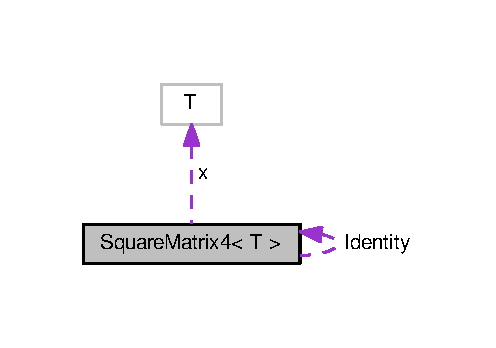
\includegraphics[width=238pt]{class_square_matrix4__coll__graph}
\end{center}
\end{figure}
\subsection*{Public Member Functions}
\begin{DoxyCompactItemize}
\item 
\+\_\+\+\_\+host\+\_\+\+\_\+ \+\_\+\+\_\+device\+\_\+\+\_\+ {\bfseries Square\+Matrix4} (T a, T b, T c, T d, T e, T f, T g, T h, T i, T j, T k, T l, T m, T n, T o, T p)\hypertarget{class_square_matrix4_a9182db1e12bd3ff20d7ccdf5ed25c156}{}\label{class_square_matrix4_a9182db1e12bd3ff20d7ccdf5ed25c156}

\item 
\+\_\+\+\_\+host\+\_\+\+\_\+ \+\_\+\+\_\+device\+\_\+\+\_\+ {\bfseries Square\+Matrix4} (const \hyperlink{class_square_matrix4}{Square\+Matrix4} \&matrix)\hypertarget{class_square_matrix4_a3d2f4a1135af79f7e86e02426abe2319}{}\label{class_square_matrix4_a3d2f4a1135af79f7e86e02426abe2319}

\item 
\+\_\+\+\_\+host\+\_\+\+\_\+ \+\_\+\+\_\+device\+\_\+\+\_\+ const T $\ast$ {\bfseries operator \mbox{[}$\,$\mbox{]}} (uint8\+\_\+t i) const\hypertarget{class_square_matrix4_af20a47c9f0b1eada3e31273d2cb76de9}{}\label{class_square_matrix4_af20a47c9f0b1eada3e31273d2cb76de9}

\item 
\+\_\+\+\_\+host\+\_\+\+\_\+ \+\_\+\+\_\+device\+\_\+\+\_\+ T $\ast$ {\bfseries operator \mbox{[}$\,$\mbox{]}} (uint8\+\_\+t i)\hypertarget{class_square_matrix4_ac748c208ebdb0090978832fae8836f0a}{}\label{class_square_matrix4_ac748c208ebdb0090978832fae8836f0a}

\item 
\+\_\+\+\_\+host\+\_\+\+\_\+ \+\_\+\+\_\+device\+\_\+\+\_\+ \hyperlink{class_square_matrix4}{Square\+Matrix4} {\bfseries operator $\ast$} (const \hyperlink{class_square_matrix4}{Square\+Matrix4} \&v) const\hypertarget{class_square_matrix4_a7cfeb42d0147390448c69b6f4ba74ee0}{}\label{class_square_matrix4_a7cfeb42d0147390448c69b6f4ba74ee0}

\item 
\+\_\+\+\_\+host\+\_\+\+\_\+ \+\_\+\+\_\+device\+\_\+\+\_\+ \hyperlink{class_square_matrix4}{Square\+Matrix4} \& {\bfseries operator $\ast$=} (const \hyperlink{class_square_matrix4}{Square\+Matrix4} \&v) const\hypertarget{class_square_matrix4_af44d511c4d55102c4f72d99692345332}{}\label{class_square_matrix4_af44d511c4d55102c4f72d99692345332}

\item 
\+\_\+\+\_\+host\+\_\+\+\_\+ \+\_\+\+\_\+device\+\_\+\+\_\+ \hyperlink{class_square_matrix4}{Square\+Matrix4} \& {\bfseries operator=} (const \hyperlink{class_square_matrix4}{Square\+Matrix4} \&matrix)\hypertarget{class_square_matrix4_a48e4130c7dc65e2ef42be5e4dbbab914}{}\label{class_square_matrix4_a48e4130c7dc65e2ef42be5e4dbbab914}

\item 
\+\_\+\+\_\+host\+\_\+\+\_\+ \+\_\+\+\_\+device\+\_\+\+\_\+ \hyperlink{class_square_matrix4}{Square\+Matrix4} \hyperlink{class_square_matrix4_a23f36c4b337c5b238b4d3fae04e6f2f0}{transposed} () const
\item 
\+\_\+\+\_\+host\+\_\+\+\_\+ \+\_\+\+\_\+device\+\_\+\+\_\+ \hyperlink{class_square_matrix4}{Square\+Matrix4} \& \hyperlink{class_square_matrix4_a7d6f675b8ae538a7c53fe1e8c390e8b3}{transpose} ()\hypertarget{class_square_matrix4_a7d6f675b8ae538a7c53fe1e8c390e8b3}{}\label{class_square_matrix4_a7d6f675b8ae538a7c53fe1e8c390e8b3}

\begin{DoxyCompactList}\small\item\em transpose itself \end{DoxyCompactList}\item 
\+\_\+\+\_\+host\+\_\+\+\_\+ \+\_\+\+\_\+device\+\_\+\+\_\+ void \hyperlink{class_square_matrix4_a96f083743422ca964d865b1034e608b4}{mul\+Point\+Mat} (const \hyperlink{class_vec3}{Vec3} \&src, \hyperlink{class_vec3}{Vec3} \&dst) const
\begin{DoxyCompactList}\small\item\em multiply point by matrix \end{DoxyCompactList}\item 
\+\_\+\+\_\+host\+\_\+\+\_\+ \+\_\+\+\_\+device\+\_\+\+\_\+ void \hyperlink{class_square_matrix4_a559765a38296c2949976c00347098fb0}{mul\+Vec\+Mat} (const \hyperlink{class_vec3}{Vec3} \&src, \hyperlink{class_vec3}{Vec3} \&dst) const
\begin{DoxyCompactList}\small\item\em multiply vector by matrix \end{DoxyCompactList}\item 
\+\_\+\+\_\+host\+\_\+\+\_\+ \+\_\+\+\_\+device\+\_\+\+\_\+ \hyperlink{class_square_matrix4}{Square\+Matrix4} {\bfseries inverse} () const\hypertarget{class_square_matrix4_a5af6eeea8a8080858fc607a7e6a25c79}{}\label{class_square_matrix4_a5af6eeea8a8080858fc607a7e6a25c79}

\item 
const \hyperlink{class_square_matrix4}{Square\+Matrix4}$<$ T $>$ \& \hyperlink{class_square_matrix4_acbf913e66c1c7b846bc25d7b2c0df31d}{invert} ()\hypertarget{class_square_matrix4_acbf913e66c1c7b846bc25d7b2c0df31d}{}\label{class_square_matrix4_acbf913e66c1c7b846bc25d7b2c0df31d}

\begin{DoxyCompactList}\small\item\em set current matrix to its inverse \end{DoxyCompactList}\item 
\+\_\+\+\_\+host\+\_\+\+\_\+ \+\_\+\+\_\+device\+\_\+\+\_\+ {\bfseries Square\+Matrix4} (T a, T b, T c, T d, T e, T f, T g, T h, T i, T j, T k, T l, T m, T n, T o, T p)\hypertarget{class_square_matrix4_a9182db1e12bd3ff20d7ccdf5ed25c156}{}\label{class_square_matrix4_a9182db1e12bd3ff20d7ccdf5ed25c156}

\item 
\+\_\+\+\_\+host\+\_\+\+\_\+ \+\_\+\+\_\+device\+\_\+\+\_\+ {\bfseries Square\+Matrix4} (const \hyperlink{class_square_matrix4}{Square\+Matrix4} \&matrix)\hypertarget{class_square_matrix4_a3d2f4a1135af79f7e86e02426abe2319}{}\label{class_square_matrix4_a3d2f4a1135af79f7e86e02426abe2319}

\item 
\+\_\+\+\_\+host\+\_\+\+\_\+ \+\_\+\+\_\+device\+\_\+\+\_\+ const T $\ast$ {\bfseries operator \mbox{[}$\,$\mbox{]}} (uint8\+\_\+t i) const\hypertarget{class_square_matrix4_af20a47c9f0b1eada3e31273d2cb76de9}{}\label{class_square_matrix4_af20a47c9f0b1eada3e31273d2cb76de9}

\item 
\+\_\+\+\_\+host\+\_\+\+\_\+ \+\_\+\+\_\+device\+\_\+\+\_\+ T $\ast$ {\bfseries operator \mbox{[}$\,$\mbox{]}} (uint8\+\_\+t i)\hypertarget{class_square_matrix4_ac748c208ebdb0090978832fae8836f0a}{}\label{class_square_matrix4_ac748c208ebdb0090978832fae8836f0a}

\item 
\+\_\+\+\_\+host\+\_\+\+\_\+ \+\_\+\+\_\+device\+\_\+\+\_\+ \hyperlink{class_square_matrix4}{Square\+Matrix4} {\bfseries operator $\ast$} (const \hyperlink{class_square_matrix4}{Square\+Matrix4} \&v) const\hypertarget{class_square_matrix4_a7cfeb42d0147390448c69b6f4ba74ee0}{}\label{class_square_matrix4_a7cfeb42d0147390448c69b6f4ba74ee0}

\item 
\+\_\+\+\_\+host\+\_\+\+\_\+ \+\_\+\+\_\+device\+\_\+\+\_\+ \hyperlink{class_square_matrix4}{Square\+Matrix4} \& {\bfseries operator $\ast$=} (const \hyperlink{class_square_matrix4}{Square\+Matrix4} \&v) const\hypertarget{class_square_matrix4_af44d511c4d55102c4f72d99692345332}{}\label{class_square_matrix4_af44d511c4d55102c4f72d99692345332}

\item 
\+\_\+\+\_\+host\+\_\+\+\_\+ \+\_\+\+\_\+device\+\_\+\+\_\+ \hyperlink{class_square_matrix4}{Square\+Matrix4} \& {\bfseries operator=} (const \hyperlink{class_square_matrix4}{Square\+Matrix4} \&matrix)\hypertarget{class_square_matrix4_a48e4130c7dc65e2ef42be5e4dbbab914}{}\label{class_square_matrix4_a48e4130c7dc65e2ef42be5e4dbbab914}

\item 
\+\_\+\+\_\+host\+\_\+\+\_\+ \+\_\+\+\_\+device\+\_\+\+\_\+ \hyperlink{class_square_matrix4}{Square\+Matrix4} \hyperlink{class_square_matrix4_a23f36c4b337c5b238b4d3fae04e6f2f0}{transposed} () const
\item 
\+\_\+\+\_\+host\+\_\+\+\_\+ \+\_\+\+\_\+device\+\_\+\+\_\+ \hyperlink{class_square_matrix4}{Square\+Matrix4} \& \hyperlink{class_square_matrix4_a7d6f675b8ae538a7c53fe1e8c390e8b3}{transpose} ()\hypertarget{class_square_matrix4_a7d6f675b8ae538a7c53fe1e8c390e8b3}{}\label{class_square_matrix4_a7d6f675b8ae538a7c53fe1e8c390e8b3}

\begin{DoxyCompactList}\small\item\em transpose itself \end{DoxyCompactList}\item 
\+\_\+\+\_\+host\+\_\+\+\_\+ \+\_\+\+\_\+device\+\_\+\+\_\+ void \hyperlink{class_square_matrix4_a96f083743422ca964d865b1034e608b4}{mul\+Point\+Mat} (const \hyperlink{class_vec3}{Vec3} \&src, \hyperlink{class_vec3}{Vec3} \&dst) const
\begin{DoxyCompactList}\small\item\em multiply point by matrix \end{DoxyCompactList}\item 
\+\_\+\+\_\+host\+\_\+\+\_\+ \+\_\+\+\_\+device\+\_\+\+\_\+ void \hyperlink{class_square_matrix4_a559765a38296c2949976c00347098fb0}{mul\+Vec\+Mat} (const \hyperlink{class_vec3}{Vec3} \&src, \hyperlink{class_vec3}{Vec3} \&dst) const
\begin{DoxyCompactList}\small\item\em multiply vector by matrix \end{DoxyCompactList}\item 
\+\_\+\+\_\+host\+\_\+\+\_\+ \+\_\+\+\_\+device\+\_\+\+\_\+ \hyperlink{class_square_matrix4}{Square\+Matrix4} {\bfseries inverse} () const\hypertarget{class_square_matrix4_a5af6eeea8a8080858fc607a7e6a25c79}{}\label{class_square_matrix4_a5af6eeea8a8080858fc607a7e6a25c79}

\item 
const \hyperlink{class_square_matrix4}{Square\+Matrix4}$<$ T $>$ \& \hyperlink{class_square_matrix4_acbf913e66c1c7b846bc25d7b2c0df31d}{invert} ()\hypertarget{class_square_matrix4_acbf913e66c1c7b846bc25d7b2c0df31d}{}\label{class_square_matrix4_acbf913e66c1c7b846bc25d7b2c0df31d}

\begin{DoxyCompactList}\small\item\em set current matrix to its inverse \end{DoxyCompactList}\end{DoxyCompactItemize}
\subsection*{Static Public Member Functions}
\begin{DoxyCompactItemize}
\item 
\+\_\+\+\_\+host\+\_\+\+\_\+ static \+\_\+\+\_\+device\+\_\+\+\_\+ void {\bfseries multiply} (const \hyperlink{class_square_matrix4}{Square\+Matrix4}$<$ T $>$ \&a, const \hyperlink{class_square_matrix4}{Square\+Matrix4} \&b, \hyperlink{class_square_matrix4}{Square\+Matrix4} \&c)\hypertarget{class_square_matrix4_a8d4381e883a6e4a7d7e2813ebc2a7af3}{}\label{class_square_matrix4_a8d4381e883a6e4a7d7e2813ebc2a7af3}

\item 
\+\_\+\+\_\+host\+\_\+\+\_\+ static \+\_\+\+\_\+device\+\_\+\+\_\+ void {\bfseries multiply} (const \hyperlink{class_square_matrix4}{Square\+Matrix4}$<$ T $>$ \&a, const \hyperlink{class_square_matrix4}{Square\+Matrix4} \&b, \hyperlink{class_square_matrix4}{Square\+Matrix4} \&c)\hypertarget{class_square_matrix4_a8d4381e883a6e4a7d7e2813ebc2a7af3}{}\label{class_square_matrix4_a8d4381e883a6e4a7d7e2813ebc2a7af3}

\end{DoxyCompactItemize}
\subsection*{Public Attributes}
\begin{DoxyCompactItemize}
\item 
T {\bfseries x} \mbox{[}4\mbox{]}\mbox{[}4\mbox{]}
\end{DoxyCompactItemize}
\subsection*{Static Public Attributes}
\begin{DoxyCompactItemize}
\item 
static const \hyperlink{class_square_matrix4}{Square\+Matrix4} {\bfseries Identity} = \hyperlink{class_square_matrix4}{Square\+Matrix4f}()\hypertarget{class_square_matrix4_a17173c29287b7d4206d9bfddb2ad8d0e}{}\label{class_square_matrix4_a17173c29287b7d4206d9bfddb2ad8d0e}

\end{DoxyCompactItemize}
\subsection*{Friends}
\begin{DoxyCompactItemize}
\item 
std\+::ostream \& {\bfseries operator$<$$<$} (std\+::ostream \&s, const \hyperlink{class_square_matrix4}{Square\+Matrix4} \&m)\hypertarget{class_square_matrix4_a548d172ab42d8b780f4c8daaf221a43e}{}\label{class_square_matrix4_a548d172ab42d8b780f4c8daaf221a43e}

\end{DoxyCompactItemize}


\subsection{Member Function Documentation}
\index{Square\+Matrix4@{Square\+Matrix4}!mul\+Point\+Mat@{mul\+Point\+Mat}}
\index{mul\+Point\+Mat@{mul\+Point\+Mat}!Square\+Matrix4@{Square\+Matrix4}}
\subsubsection[{\texorpdfstring{mul\+Point\+Mat(const Vec3 \&src, Vec3 \&dst) const}{mulPointMat(const Vec3 \&src, Vec3 \&dst) const}}]{\setlength{\rightskip}{0pt plus 5cm}template$<$typename T$>$ \+\_\+\+\_\+host\+\_\+\+\_\+ \+\_\+\+\_\+device\+\_\+\+\_\+ void {\bf Square\+Matrix4}$<$ T $>$\+::mul\+Point\+Mat (
\begin{DoxyParamCaption}
\item[{const {\bf Vec3} \&}]{src, }
\item[{{\bf Vec3} \&}]{dst}
\end{DoxyParamCaption}
) const\hspace{0.3cm}{\ttfamily [inline]}}\hypertarget{class_square_matrix4_a96f083743422ca964d865b1034e608b4}{}\label{class_square_matrix4_a96f083743422ca964d865b1034e608b4}


multiply point by matrix 


\begin{DoxyParams}[1]{Parameters}
\mbox{\tt in}  & {\em src} & -\/ vector multyplied by a matrix \\
\hline
\mbox{\tt out}  & {\em dst} & -\/ output vector \\
\hline
\end{DoxyParams}
Here is the caller graph for this function\+:
\nopagebreak
\begin{figure}[H]
\begin{center}
\leavevmode
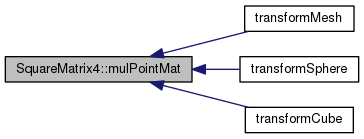
\includegraphics[width=345pt]{class_square_matrix4_a96f083743422ca964d865b1034e608b4_icgraph}
\end{center}
\end{figure}
\index{Square\+Matrix4@{Square\+Matrix4}!mul\+Point\+Mat@{mul\+Point\+Mat}}
\index{mul\+Point\+Mat@{mul\+Point\+Mat}!Square\+Matrix4@{Square\+Matrix4}}
\subsubsection[{\texorpdfstring{mul\+Point\+Mat(const Vec3 \&src, Vec3 \&dst) const}{mulPointMat(const Vec3 \&src, Vec3 \&dst) const}}]{\setlength{\rightskip}{0pt plus 5cm}template$<$typename T$>$ \+\_\+\+\_\+host\+\_\+\+\_\+ \+\_\+\+\_\+device\+\_\+\+\_\+ void {\bf Square\+Matrix4}$<$ T $>$\+::mul\+Point\+Mat (
\begin{DoxyParamCaption}
\item[{const {\bf Vec3} \&}]{src, }
\item[{{\bf Vec3} \&}]{dst}
\end{DoxyParamCaption}
) const\hspace{0.3cm}{\ttfamily [inline]}}\hypertarget{class_square_matrix4_a96f083743422ca964d865b1034e608b4}{}\label{class_square_matrix4_a96f083743422ca964d865b1034e608b4}


multiply point by matrix 


\begin{DoxyParams}[1]{Parameters}
\mbox{\tt in}  & {\em src} & -\/ vector multyplied by a matrix \\
\hline
\mbox{\tt out}  & {\em dst} & -\/ output vector \\
\hline
\end{DoxyParams}
\index{Square\+Matrix4@{Square\+Matrix4}!mul\+Vec\+Mat@{mul\+Vec\+Mat}}
\index{mul\+Vec\+Mat@{mul\+Vec\+Mat}!Square\+Matrix4@{Square\+Matrix4}}
\subsubsection[{\texorpdfstring{mul\+Vec\+Mat(const Vec3 \&src, Vec3 \&dst) const}{mulVecMat(const Vec3 \&src, Vec3 \&dst) const}}]{\setlength{\rightskip}{0pt plus 5cm}template$<$typename T$>$ \+\_\+\+\_\+host\+\_\+\+\_\+ \+\_\+\+\_\+device\+\_\+\+\_\+ void {\bf Square\+Matrix4}$<$ T $>$\+::mul\+Vec\+Mat (
\begin{DoxyParamCaption}
\item[{const {\bf Vec3} \&}]{src, }
\item[{{\bf Vec3} \&}]{dst}
\end{DoxyParamCaption}
) const\hspace{0.3cm}{\ttfamily [inline]}}\hypertarget{class_square_matrix4_a559765a38296c2949976c00347098fb0}{}\label{class_square_matrix4_a559765a38296c2949976c00347098fb0}


multiply vector by matrix 


\begin{DoxyParams}[1]{Parameters}
\mbox{\tt in}  & {\em src} & -\/ vector multyplied by a matrix \\
\hline
\mbox{\tt out}  & {\em dst} & -\/ output vector \\
\hline
\end{DoxyParams}
\index{Square\+Matrix4@{Square\+Matrix4}!mul\+Vec\+Mat@{mul\+Vec\+Mat}}
\index{mul\+Vec\+Mat@{mul\+Vec\+Mat}!Square\+Matrix4@{Square\+Matrix4}}
\subsubsection[{\texorpdfstring{mul\+Vec\+Mat(const Vec3 \&src, Vec3 \&dst) const}{mulVecMat(const Vec3 \&src, Vec3 \&dst) const}}]{\setlength{\rightskip}{0pt plus 5cm}template$<$typename T$>$ \+\_\+\+\_\+host\+\_\+\+\_\+ \+\_\+\+\_\+device\+\_\+\+\_\+ void {\bf Square\+Matrix4}$<$ T $>$\+::mul\+Vec\+Mat (
\begin{DoxyParamCaption}
\item[{const {\bf Vec3} \&}]{src, }
\item[{{\bf Vec3} \&}]{dst}
\end{DoxyParamCaption}
) const\hspace{0.3cm}{\ttfamily [inline]}}\hypertarget{class_square_matrix4_a559765a38296c2949976c00347098fb0}{}\label{class_square_matrix4_a559765a38296c2949976c00347098fb0}


multiply vector by matrix 


\begin{DoxyParams}[1]{Parameters}
\mbox{\tt in}  & {\em src} & -\/ vector multyplied by a matrix \\
\hline
\mbox{\tt out}  & {\em dst} & -\/ output vector \\
\hline
\end{DoxyParams}
\index{Square\+Matrix4@{Square\+Matrix4}!transposed@{transposed}}
\index{transposed@{transposed}!Square\+Matrix4@{Square\+Matrix4}}
\subsubsection[{\texorpdfstring{transposed() const}{transposed() const}}]{\setlength{\rightskip}{0pt plus 5cm}template$<$typename T$>$ \+\_\+\+\_\+host\+\_\+\+\_\+ \+\_\+\+\_\+device\+\_\+\+\_\+ {\bf Square\+Matrix4} {\bf Square\+Matrix4}$<$ T $>$\+::transposed (
\begin{DoxyParamCaption}
{}
\end{DoxyParamCaption}
) const\hspace{0.3cm}{\ttfamily [inline]}}\hypertarget{class_square_matrix4_a23f36c4b337c5b238b4d3fae04e6f2f0}{}\label{class_square_matrix4_a23f36c4b337c5b238b4d3fae04e6f2f0}
return a transposed copy of the current matrix as a new matrix \index{Square\+Matrix4@{Square\+Matrix4}!transposed@{transposed}}
\index{transposed@{transposed}!Square\+Matrix4@{Square\+Matrix4}}
\subsubsection[{\texorpdfstring{transposed() const}{transposed() const}}]{\setlength{\rightskip}{0pt plus 5cm}template$<$typename T$>$ \+\_\+\+\_\+host\+\_\+\+\_\+ \+\_\+\+\_\+device\+\_\+\+\_\+ {\bf Square\+Matrix4} {\bf Square\+Matrix4}$<$ T $>$\+::transposed (
\begin{DoxyParamCaption}
{}
\end{DoxyParamCaption}
) const\hspace{0.3cm}{\ttfamily [inline]}}\hypertarget{class_square_matrix4_a23f36c4b337c5b238b4d3fae04e6f2f0}{}\label{class_square_matrix4_a23f36c4b337c5b238b4d3fae04e6f2f0}
return a transposed copy of the current matrix as a new matrix 

\subsection{Member Data Documentation}
\index{Square\+Matrix4@{Square\+Matrix4}!x@{x}}
\index{x@{x}!Square\+Matrix4@{Square\+Matrix4}}
\subsubsection[{\texorpdfstring{x}{x}}]{\setlength{\rightskip}{0pt plus 5cm}template$<$typename T$>$ T {\bf Square\+Matrix4}$<$ T $>$\+::x}\hypertarget{class_square_matrix4_a8cd2e4d89a53a6cb802606054fb0c1ff}{}\label{class_square_matrix4_a8cd2e4d89a53a6cb802606054fb0c1ff}
{\bfseries Initial value\+:}
\begin{DoxyCode}
= \{ \{1,0,0,0\}
                 ,\{0,1,0,0\}
                 ,\{0,0,1,0\}
                 ,\{0,0,0,1\} \}
\end{DoxyCode}


The documentation for this class was generated from the following files\+:\begin{DoxyCompactItemize}
\item 
/home/god/cuda-\/workspace/r\+T\+Tracer/include/\hyperlink{r_t_tracer_2include_2geom_8cuh}{geom.\+cuh}\item 
/home/god/cuda-\/workspace/r\+T\+Tracer/source/main.\+cu\end{DoxyCompactItemize}

\hypertarget{class_triangle}{}\section{Triangle Class Reference}
\label{class_triangle}\index{Triangle@{Triangle}}
\subsection*{Public Member Functions}
\begin{DoxyCompactItemize}
\item 
{\bfseries Triangle} (uint32\+\_\+t v0, uint32\+\_\+t v1, uint32\+\_\+t v2)\hypertarget{class_triangle_a8532ce36a26abc9ab0064533ee880b67}{}\label{class_triangle_a8532ce36a26abc9ab0064533ee880b67}

\item 
\+\_\+\+\_\+host\+\_\+\+\_\+ \+\_\+\+\_\+device\+\_\+\+\_\+ uint32\+\_\+t $\ast$ {\bfseries data} ()\hypertarget{class_triangle_a100d35fe94ff02922981eabe1730f9f4}{}\label{class_triangle_a100d35fe94ff02922981eabe1730f9f4}

\item 
\+\_\+\+\_\+host\+\_\+\+\_\+ \+\_\+\+\_\+device\+\_\+\+\_\+ const uint32\+\_\+t \& {\bfseries operator\mbox{[}$\,$\mbox{]}} (size\+\_\+t i) const\hypertarget{class_triangle_a9ac6b64d26db74a4227eca4a0b3a437b}{}\label{class_triangle_a9ac6b64d26db74a4227eca4a0b3a437b}

\item 
\+\_\+\+\_\+host\+\_\+\+\_\+ \+\_\+\+\_\+device\+\_\+\+\_\+ uint32\+\_\+t \& {\bfseries operator\mbox{[}$\,$\mbox{]}} (size\+\_\+t i)\hypertarget{class_triangle_a51ae109c4a21132769252965eb4745e8}{}\label{class_triangle_a51ae109c4a21132769252965eb4745e8}

\item 
\+\_\+\+\_\+host\+\_\+\+\_\+ \+\_\+\+\_\+device\+\_\+\+\_\+ const \hyperlink{class_triangle}{Triangle} \& {\bfseries operator=} (const \hyperlink{class_triangle}{Triangle} \&tr)\hypertarget{class_triangle_a957601b66c9bc185e081a9c0b16a11ad}{}\label{class_triangle_a957601b66c9bc185e081a9c0b16a11ad}

\item 
\+\_\+\+\_\+host\+\_\+\+\_\+ \+\_\+\+\_\+device\+\_\+\+\_\+ bool {\bfseries hit} (\hyperlink{class_ray}{Ray} \&r, const \hyperlink{class_vec3}{Vec3f} $\ast$verts, float \&u, float \&v)\hypertarget{class_triangle_a853b6db440f108fe7581e2fc8a90bdc9}{}\label{class_triangle_a853b6db440f108fe7581e2fc8a90bdc9}

\end{DoxyCompactItemize}


The documentation for this class was generated from the following files\+:\begin{DoxyCompactItemize}
\item 
/home/god/cuda-\/workspace/r\+T\+Tracer/include/\hyperlink{geom_8cuh}{geom.\+cuh}\item 
/home/god/cuda-\/workspace/r\+T\+Tracer/source/geom.\+cu\end{DoxyCompactItemize}

\hypertarget{class_vec2}{}\section{Vec2 Class Reference}
\label{class_vec2}\index{Vec2@{Vec2}}
\subsection*{Public Member Functions}
\begin{DoxyCompactItemize}
\item 
\+\_\+\+\_\+host\+\_\+\+\_\+ \+\_\+\+\_\+device\+\_\+\+\_\+ {\bfseries Vec2} (const float \&xx)\hypertarget{class_vec2_a33d3d56000bb864e5d30eb48f1685695}{}\label{class_vec2_a33d3d56000bb864e5d30eb48f1685695}

\item 
\+\_\+\+\_\+host\+\_\+\+\_\+ \+\_\+\+\_\+device\+\_\+\+\_\+ {\bfseries Vec2} (float xx, float yy)\hypertarget{class_vec2_aa39cf936ef3699647eb72ef76f6ce97d}{}\label{class_vec2_aa39cf936ef3699647eb72ef76f6ce97d}

\item 
\+\_\+\+\_\+host\+\_\+\+\_\+ \+\_\+\+\_\+device\+\_\+\+\_\+ {\bfseries Vec2} (const \hyperlink{class_vec2}{Vec2} \&v)\hypertarget{class_vec2_a0dfcf0539532615ae5b37a4d2995253d}{}\label{class_vec2_a0dfcf0539532615ae5b37a4d2995253d}

\item 
\+\_\+\+\_\+host\+\_\+\+\_\+ \+\_\+\+\_\+device\+\_\+\+\_\+ \hyperlink{class_vec2}{Vec2} {\bfseries operator+} (const \hyperlink{class_vec2}{Vec2} \&v) const\hypertarget{class_vec2_a71daf354e7f2dc8acd0f4ccb33e2d77b}{}\label{class_vec2_a71daf354e7f2dc8acd0f4ccb33e2d77b}

\item 
\hyperlink{class_vec2}{Vec2} {\bfseries operator/} (const float \&r) const\hypertarget{class_vec2_a71b95a0b8cb412cf5d7fc52b53dc8e47}{}\label{class_vec2_a71b95a0b8cb412cf5d7fc52b53dc8e47}

\item 
\+\_\+\+\_\+host\+\_\+\+\_\+ \+\_\+\+\_\+device\+\_\+\+\_\+ \hyperlink{class_vec2}{Vec2} {\bfseries operator $\ast$} (const float \&r) const\hypertarget{class_vec2_a3eae44cc4053ef70be638d4d4202fe72}{}\label{class_vec2_a3eae44cc4053ef70be638d4d4202fe72}

\item 
\+\_\+\+\_\+host\+\_\+\+\_\+ \+\_\+\+\_\+device\+\_\+\+\_\+ \hyperlink{class_vec2}{Vec2} \& {\bfseries operator/=} (const float \&r)\hypertarget{class_vec2_a622c47d2f678a364b2cc6d09a453cfd6}{}\label{class_vec2_a622c47d2f678a364b2cc6d09a453cfd6}

\item 
\+\_\+\+\_\+host\+\_\+\+\_\+ \+\_\+\+\_\+device\+\_\+\+\_\+ \hyperlink{class_vec2}{Vec2} \& {\bfseries operator $\ast$=} (const float \&r)\hypertarget{class_vec2_ab7f2a84b847c04690ddd7823144ae591}{}\label{class_vec2_ab7f2a84b847c04690ddd7823144ae591}

\item 
\+\_\+\+\_\+host\+\_\+\+\_\+ \+\_\+\+\_\+device\+\_\+\+\_\+ void {\bfseries swap} (\hyperlink{class_vec2}{Vec2} \&vec)\hypertarget{class_vec2_a45e2ef0b091128f3d78fc691b862cdef}{}\label{class_vec2_a45e2ef0b091128f3d78fc691b862cdef}

\item 
\+\_\+\+\_\+host\+\_\+\+\_\+ \+\_\+\+\_\+device\+\_\+\+\_\+ {\bfseries Vec2} (const float \&xx)\hypertarget{class_vec2_a33d3d56000bb864e5d30eb48f1685695}{}\label{class_vec2_a33d3d56000bb864e5d30eb48f1685695}

\item 
\+\_\+\+\_\+host\+\_\+\+\_\+ \+\_\+\+\_\+device\+\_\+\+\_\+ {\bfseries Vec2} (float xx, float yy)\hypertarget{class_vec2_aa39cf936ef3699647eb72ef76f6ce97d}{}\label{class_vec2_aa39cf936ef3699647eb72ef76f6ce97d}

\item 
\+\_\+\+\_\+host\+\_\+\+\_\+ \+\_\+\+\_\+device\+\_\+\+\_\+ {\bfseries Vec2} (const \hyperlink{class_vec2}{Vec2} \&v)\hypertarget{class_vec2_a0dfcf0539532615ae5b37a4d2995253d}{}\label{class_vec2_a0dfcf0539532615ae5b37a4d2995253d}

\item 
\+\_\+\+\_\+host\+\_\+\+\_\+ \+\_\+\+\_\+device\+\_\+\+\_\+ \hyperlink{class_vec2}{Vec2} {\bfseries operator+} (const \hyperlink{class_vec2}{Vec2} \&v) const\hypertarget{class_vec2_a71daf354e7f2dc8acd0f4ccb33e2d77b}{}\label{class_vec2_a71daf354e7f2dc8acd0f4ccb33e2d77b}

\item 
\hyperlink{class_vec2}{Vec2} {\bfseries operator/} (const float \&r) const\hypertarget{class_vec2_a71b95a0b8cb412cf5d7fc52b53dc8e47}{}\label{class_vec2_a71b95a0b8cb412cf5d7fc52b53dc8e47}

\item 
\+\_\+\+\_\+host\+\_\+\+\_\+ \+\_\+\+\_\+device\+\_\+\+\_\+ \hyperlink{class_vec2}{Vec2} {\bfseries operator $\ast$} (const float \&r) const\hypertarget{class_vec2_a3eae44cc4053ef70be638d4d4202fe72}{}\label{class_vec2_a3eae44cc4053ef70be638d4d4202fe72}

\item 
\+\_\+\+\_\+host\+\_\+\+\_\+ \+\_\+\+\_\+device\+\_\+\+\_\+ \hyperlink{class_vec2}{Vec2} \& {\bfseries operator/=} (const float \&r)\hypertarget{class_vec2_a622c47d2f678a364b2cc6d09a453cfd6}{}\label{class_vec2_a622c47d2f678a364b2cc6d09a453cfd6}

\item 
\+\_\+\+\_\+host\+\_\+\+\_\+ \+\_\+\+\_\+device\+\_\+\+\_\+ \hyperlink{class_vec2}{Vec2} \& {\bfseries operator $\ast$=} (const float \&r)\hypertarget{class_vec2_ab7f2a84b847c04690ddd7823144ae591}{}\label{class_vec2_ab7f2a84b847c04690ddd7823144ae591}

\item 
\+\_\+\+\_\+host\+\_\+\+\_\+ \+\_\+\+\_\+device\+\_\+\+\_\+ void {\bfseries swap} (\hyperlink{class_vec2}{Vec2} \&vec)\hypertarget{class_vec2_a45e2ef0b091128f3d78fc691b862cdef}{}\label{class_vec2_a45e2ef0b091128f3d78fc691b862cdef}

\end{DoxyCompactItemize}
\subsection*{Public Attributes}
\begin{DoxyCompactItemize}
\item 
float2 {\bfseries xy}\hypertarget{class_vec2_ae166edaf1b05eb0634e8ceb08adf1cc3}{}\label{class_vec2_ae166edaf1b05eb0634e8ceb08adf1cc3}

\end{DoxyCompactItemize}
\subsection*{Friends}
\begin{DoxyCompactItemize}
\item 
std\+::ostream \& {\bfseries operator$<$$<$} (std\+::ostream \&s, const \hyperlink{class_vec2}{Vec2} \&v)\hypertarget{class_vec2_a694960aa6f1e1475c532ec7682f39287}{}\label{class_vec2_a694960aa6f1e1475c532ec7682f39287}

\item 
\+\_\+\+\_\+host\+\_\+\+\_\+ \+\_\+\+\_\+device\+\_\+\+\_\+ friend \hyperlink{class_vec2}{Vec2} {\bfseries operator $\ast$} (const float \&r, const \hyperlink{class_vec2}{Vec2} \&v)\hypertarget{class_vec2_a85b03ac25ec19d9bb9b746474b443d17}{}\label{class_vec2_a85b03ac25ec19d9bb9b746474b443d17}

\item 
\+\_\+\+\_\+host\+\_\+\+\_\+ \+\_\+\+\_\+device\+\_\+\+\_\+ friend \hyperlink{class_vec2}{Vec2} {\bfseries operator/} (const float \&r, const \hyperlink{class_vec2}{Vec2} \&v)\hypertarget{class_vec2_ae7585370defee85ee50ac0ccb82f5e49}{}\label{class_vec2_ae7585370defee85ee50ac0ccb82f5e49}

\item 
std\+::ostream \& {\bfseries operator$<$$<$} (std\+::ostream \&s, const \hyperlink{class_vec2}{Vec2} \&v)\hypertarget{class_vec2_a694960aa6f1e1475c532ec7682f39287}{}\label{class_vec2_a694960aa6f1e1475c532ec7682f39287}

\item 
\+\_\+\+\_\+host\+\_\+\+\_\+ \+\_\+\+\_\+device\+\_\+\+\_\+ friend \hyperlink{class_vec2}{Vec2} {\bfseries operator $\ast$} (const float \&r, const \hyperlink{class_vec2}{Vec2} \&v)\hypertarget{class_vec2_a85b03ac25ec19d9bb9b746474b443d17}{}\label{class_vec2_a85b03ac25ec19d9bb9b746474b443d17}

\item 
\+\_\+\+\_\+host\+\_\+\+\_\+ \+\_\+\+\_\+device\+\_\+\+\_\+ friend \hyperlink{class_vec2}{Vec2} {\bfseries operator/} (const float \&r, const \hyperlink{class_vec2}{Vec2} \&v)\hypertarget{class_vec2_ae7585370defee85ee50ac0ccb82f5e49}{}\label{class_vec2_ae7585370defee85ee50ac0ccb82f5e49}

\end{DoxyCompactItemize}


The documentation for this class was generated from the following file\+:\begin{DoxyCompactItemize}
\item 
/home/god/cuda-\/workspace/r\+T\+Tracer/include/\hyperlink{r_t_tracer_2include_2geom_8cuh}{geom.\+cuh}\end{DoxyCompactItemize}

\hypertarget{class_vec3}{}\section{Vec3 Class Reference}
\label{class_vec3}\index{Vec3@{Vec3}}
\subsection*{Public Member Functions}
\begin{DoxyCompactItemize}
\item 
\+\_\+\+\_\+host\+\_\+\+\_\+ \+\_\+\+\_\+device\+\_\+\+\_\+ {\bfseries Vec3} (float xx)\hypertarget{class_vec3_ab76e7b1dfb13878ef79e295bb4e7444b}{}\label{class_vec3_ab76e7b1dfb13878ef79e295bb4e7444b}

\item 
\+\_\+\+\_\+host\+\_\+\+\_\+ \+\_\+\+\_\+device\+\_\+\+\_\+ {\bfseries Vec3} (float xx, float yy, float zz)\hypertarget{class_vec3_a7d4737059c28fa7c8c3db22ba4718178}{}\label{class_vec3_a7d4737059c28fa7c8c3db22ba4718178}

\item 
\+\_\+\+\_\+host\+\_\+\+\_\+ \+\_\+\+\_\+device\+\_\+\+\_\+ {\bfseries Vec3} (const \hyperlink{class_vec3}{Vec3} \&vec)\hypertarget{class_vec3_a3b08c22982decc110fb443cad3bc7eac}{}\label{class_vec3_a3b08c22982decc110fb443cad3bc7eac}

\item 
\+\_\+\+\_\+host\+\_\+\+\_\+ \+\_\+\+\_\+device\+\_\+\+\_\+ {\bfseries Vec3} (const float3 \&vec)\hypertarget{class_vec3_a2edb8ba8713360b31ef22fa301681003}{}\label{class_vec3_a2edb8ba8713360b31ef22fa301681003}

\item 
\+\_\+\+\_\+host\+\_\+\+\_\+ \+\_\+\+\_\+device\+\_\+\+\_\+ {\bfseries Vec3} (const float4 \&vec)\hypertarget{class_vec3_aee1b03c9e5b951fb7b5b9171db699057}{}\label{class_vec3_aee1b03c9e5b951fb7b5b9171db699057}

\item 
\+\_\+\+\_\+host\+\_\+\+\_\+ \+\_\+\+\_\+device\+\_\+\+\_\+ float \& {\bfseries operator \mbox{[}$\,$\mbox{]}} (uint8\+\_\+t i)\hypertarget{class_vec3_a13f7dfd7a5bcea529e57f1b7fd1a45f5}{}\label{class_vec3_a13f7dfd7a5bcea529e57f1b7fd1a45f5}

\item 
\+\_\+\+\_\+host\+\_\+\+\_\+ \+\_\+\+\_\+device\+\_\+\+\_\+ const float \& {\bfseries operator \mbox{[}$\,$\mbox{]}} (uint8\+\_\+t i) const\hypertarget{class_vec3_acb50b12a71971b8229a0e81352ef848f}{}\label{class_vec3_acb50b12a71971b8229a0e81352ef848f}

\item 
\+\_\+\+\_\+host\+\_\+\+\_\+ \+\_\+\+\_\+device\+\_\+\+\_\+ \hyperlink{class_vec3}{Vec3} {\bfseries operator+} (const \hyperlink{class_vec3}{Vec3} \&v) const\hypertarget{class_vec3_aa60e8d896fff309c4b0ee1435b6e00bb}{}\label{class_vec3_aa60e8d896fff309c4b0ee1435b6e00bb}

\item 
\+\_\+\+\_\+host\+\_\+\+\_\+ \+\_\+\+\_\+device\+\_\+\+\_\+ \hyperlink{class_vec3}{Vec3} \& {\bfseries operator+=} (const \hyperlink{class_vec3}{Vec3} \&v)\hypertarget{class_vec3_a6f4e538fda1288a1c650407dcaa2e4ad}{}\label{class_vec3_a6f4e538fda1288a1c650407dcaa2e4ad}

\item 
\+\_\+\+\_\+host\+\_\+\+\_\+ \+\_\+\+\_\+device\+\_\+\+\_\+ \hyperlink{class_vec3}{Vec3} {\bfseries operator -\/} (const \hyperlink{class_vec3}{Vec3} \&v) const\hypertarget{class_vec3_aca45728410c7fa3cfc10168e41ab4649}{}\label{class_vec3_aca45728410c7fa3cfc10168e41ab4649}

\item 
\+\_\+\+\_\+host\+\_\+\+\_\+ \+\_\+\+\_\+device\+\_\+\+\_\+ \hyperlink{class_vec3}{Vec3} {\bfseries operator -\/} () const\hypertarget{class_vec3_ab8ef4a52f843e1381c3f22c6cd61fcc9}{}\label{class_vec3_ab8ef4a52f843e1381c3f22c6cd61fcc9}

\item 
\+\_\+\+\_\+host\+\_\+\+\_\+ \+\_\+\+\_\+device\+\_\+\+\_\+ \hyperlink{class_vec3}{Vec3} {\bfseries operator $\ast$} (const float \&r) const\hypertarget{class_vec3_a0fd3d63acd5e4ebbe2f8dda2825869fc}{}\label{class_vec3_a0fd3d63acd5e4ebbe2f8dda2825869fc}

\item 
\+\_\+\+\_\+host\+\_\+\+\_\+ \+\_\+\+\_\+device\+\_\+\+\_\+ \hyperlink{class_vec3}{Vec3} {\bfseries operator $\ast$=} (const float \&r) const\hypertarget{class_vec3_aaa0e591b69a2cf5d585e9d048d0c20f4}{}\label{class_vec3_aaa0e591b69a2cf5d585e9d048d0c20f4}

\item 
\+\_\+\+\_\+host\+\_\+\+\_\+ \+\_\+\+\_\+device\+\_\+\+\_\+ \hyperlink{class_vec3}{Vec3} {\bfseries operator $\ast$} (const \hyperlink{class_vec3}{Vec3} \&v) const\hypertarget{class_vec3_a2f1d4dcb982ffdc48e9c87d4d8a7655f}{}\label{class_vec3_a2f1d4dcb982ffdc48e9c87d4d8a7655f}

\item 
\+\_\+\+\_\+host\+\_\+\+\_\+ \+\_\+\+\_\+device\+\_\+\+\_\+ \hyperlink{class_vec3}{Vec3} {\bfseries operator/} (const float \&r) const\hypertarget{class_vec3_a9b66d38d3386efcfca935e2a90a95aa6}{}\label{class_vec3_a9b66d38d3386efcfca935e2a90a95aa6}

\item 
\+\_\+\+\_\+host\+\_\+\+\_\+ \+\_\+\+\_\+device\+\_\+\+\_\+ \hyperlink{class_vec3}{Vec3} \& {\bfseries operator=} (const \hyperlink{class_vec3}{Vec3} \&vec)\hypertarget{class_vec3_abd0c90cf6cc28577248e9ae86d72d5a9}{}\label{class_vec3_abd0c90cf6cc28577248e9ae86d72d5a9}

\item 
\+\_\+\+\_\+host\+\_\+\+\_\+ \+\_\+\+\_\+device\+\_\+\+\_\+ {\bfseries operator float3} () const\hypertarget{class_vec3_afa3f84872dfa8c04bed556854730e6a9}{}\label{class_vec3_afa3f84872dfa8c04bed556854730e6a9}

\item 
\+\_\+\+\_\+host\+\_\+\+\_\+ \+\_\+\+\_\+device\+\_\+\+\_\+ float {\bfseries length} () const\hypertarget{class_vec3_a12cbc93353a9dc6c9ea5e4b2977fc865}{}\label{class_vec3_a12cbc93353a9dc6c9ea5e4b2977fc865}

\item 
\+\_\+\+\_\+host\+\_\+\+\_\+ \+\_\+\+\_\+device\+\_\+\+\_\+ \hyperlink{class_vec3}{Vec3} \& {\bfseries normalize} ()\hypertarget{class_vec3_aaeb17c15d3cbdc7e3d8981b7f0f49b51}{}\label{class_vec3_aaeb17c15d3cbdc7e3d8981b7f0f49b51}

\item 
\+\_\+\+\_\+host\+\_\+\+\_\+ \+\_\+\+\_\+device\+\_\+\+\_\+ \hyperlink{class_vec3}{Vec3} {\bfseries cross} (const \hyperlink{class_vec3}{Vec3} \&v) const\hypertarget{class_vec3_a7dbe7c404cdda8d7f40c398b2fd2eeba}{}\label{class_vec3_a7dbe7c404cdda8d7f40c398b2fd2eeba}

\item 
\+\_\+\+\_\+host\+\_\+\+\_\+ \+\_\+\+\_\+device\+\_\+\+\_\+ float {\bfseries dot} (const \hyperlink{class_vec3}{Vec3} \&v) const\hypertarget{class_vec3_aabc0167d8027104b5b9d7380cdda9b66}{}\label{class_vec3_aabc0167d8027104b5b9d7380cdda9b66}

\item 
\+\_\+\+\_\+host\+\_\+\+\_\+ \+\_\+\+\_\+device\+\_\+\+\_\+ void {\bfseries swap} (\hyperlink{class_vec3}{Vec3} \&vec)\hypertarget{class_vec3_a03632ba5412c9f2048004e2f208d7bb4}{}\label{class_vec3_a03632ba5412c9f2048004e2f208d7bb4}

\item 
\+\_\+\+\_\+host\+\_\+\+\_\+ \+\_\+\+\_\+device\+\_\+\+\_\+ {\bfseries Vec3} (float xx)\hypertarget{class_vec3_ab76e7b1dfb13878ef79e295bb4e7444b}{}\label{class_vec3_ab76e7b1dfb13878ef79e295bb4e7444b}

\item 
\+\_\+\+\_\+host\+\_\+\+\_\+ \+\_\+\+\_\+device\+\_\+\+\_\+ {\bfseries Vec3} (float xx, float yy, float zz)\hypertarget{class_vec3_a7d4737059c28fa7c8c3db22ba4718178}{}\label{class_vec3_a7d4737059c28fa7c8c3db22ba4718178}

\item 
\+\_\+\+\_\+host\+\_\+\+\_\+ \+\_\+\+\_\+device\+\_\+\+\_\+ {\bfseries Vec3} (const \hyperlink{class_vec3}{Vec3} \&vec)\hypertarget{class_vec3_a3b08c22982decc110fb443cad3bc7eac}{}\label{class_vec3_a3b08c22982decc110fb443cad3bc7eac}

\item 
\+\_\+\+\_\+host\+\_\+\+\_\+ \+\_\+\+\_\+device\+\_\+\+\_\+ {\bfseries Vec3} (const float3 \&vec)\hypertarget{class_vec3_a2edb8ba8713360b31ef22fa301681003}{}\label{class_vec3_a2edb8ba8713360b31ef22fa301681003}

\item 
\+\_\+\+\_\+host\+\_\+\+\_\+ \+\_\+\+\_\+device\+\_\+\+\_\+ {\bfseries Vec3} (const float4 \&vec)\hypertarget{class_vec3_aee1b03c9e5b951fb7b5b9171db699057}{}\label{class_vec3_aee1b03c9e5b951fb7b5b9171db699057}

\item 
\+\_\+\+\_\+host\+\_\+\+\_\+ \+\_\+\+\_\+device\+\_\+\+\_\+ float \& {\bfseries operator \mbox{[}$\,$\mbox{]}} (uint8\+\_\+t i)\hypertarget{class_vec3_a13f7dfd7a5bcea529e57f1b7fd1a45f5}{}\label{class_vec3_a13f7dfd7a5bcea529e57f1b7fd1a45f5}

\item 
\+\_\+\+\_\+host\+\_\+\+\_\+ \+\_\+\+\_\+device\+\_\+\+\_\+ const float \& {\bfseries operator \mbox{[}$\,$\mbox{]}} (uint8\+\_\+t i) const\hypertarget{class_vec3_acb50b12a71971b8229a0e81352ef848f}{}\label{class_vec3_acb50b12a71971b8229a0e81352ef848f}

\item 
\+\_\+\+\_\+host\+\_\+\+\_\+ \+\_\+\+\_\+device\+\_\+\+\_\+ \hyperlink{class_vec3}{Vec3} {\bfseries operator+} (const \hyperlink{class_vec3}{Vec3} \&v) const\hypertarget{class_vec3_aa60e8d896fff309c4b0ee1435b6e00bb}{}\label{class_vec3_aa60e8d896fff309c4b0ee1435b6e00bb}

\item 
\+\_\+\+\_\+host\+\_\+\+\_\+ \+\_\+\+\_\+device\+\_\+\+\_\+ \hyperlink{class_vec3}{Vec3} \& {\bfseries operator+=} (const \hyperlink{class_vec3}{Vec3} \&v)\hypertarget{class_vec3_a6f4e538fda1288a1c650407dcaa2e4ad}{}\label{class_vec3_a6f4e538fda1288a1c650407dcaa2e4ad}

\item 
\+\_\+\+\_\+host\+\_\+\+\_\+ \+\_\+\+\_\+device\+\_\+\+\_\+ \hyperlink{class_vec3}{Vec3} {\bfseries operator -\/} (const \hyperlink{class_vec3}{Vec3} \&v) const\hypertarget{class_vec3_aca45728410c7fa3cfc10168e41ab4649}{}\label{class_vec3_aca45728410c7fa3cfc10168e41ab4649}

\item 
\+\_\+\+\_\+host\+\_\+\+\_\+ \+\_\+\+\_\+device\+\_\+\+\_\+ \hyperlink{class_vec3}{Vec3} {\bfseries operator -\/} () const\hypertarget{class_vec3_ab8ef4a52f843e1381c3f22c6cd61fcc9}{}\label{class_vec3_ab8ef4a52f843e1381c3f22c6cd61fcc9}

\item 
\+\_\+\+\_\+host\+\_\+\+\_\+ \+\_\+\+\_\+device\+\_\+\+\_\+ \hyperlink{class_vec3}{Vec3} {\bfseries operator $\ast$} (const float \&r) const\hypertarget{class_vec3_a0fd3d63acd5e4ebbe2f8dda2825869fc}{}\label{class_vec3_a0fd3d63acd5e4ebbe2f8dda2825869fc}

\item 
\+\_\+\+\_\+host\+\_\+\+\_\+ \+\_\+\+\_\+device\+\_\+\+\_\+ \hyperlink{class_vec3}{Vec3} {\bfseries operator $\ast$=} (const float \&r) const\hypertarget{class_vec3_aaa0e591b69a2cf5d585e9d048d0c20f4}{}\label{class_vec3_aaa0e591b69a2cf5d585e9d048d0c20f4}

\item 
\+\_\+\+\_\+host\+\_\+\+\_\+ \+\_\+\+\_\+device\+\_\+\+\_\+ \hyperlink{class_vec3}{Vec3} {\bfseries operator $\ast$} (const \hyperlink{class_vec3}{Vec3} \&v) const\hypertarget{class_vec3_a2f1d4dcb982ffdc48e9c87d4d8a7655f}{}\label{class_vec3_a2f1d4dcb982ffdc48e9c87d4d8a7655f}

\item 
\+\_\+\+\_\+host\+\_\+\+\_\+ \+\_\+\+\_\+device\+\_\+\+\_\+ \hyperlink{class_vec3}{Vec3} {\bfseries operator/} (const float \&r) const\hypertarget{class_vec3_a9b66d38d3386efcfca935e2a90a95aa6}{}\label{class_vec3_a9b66d38d3386efcfca935e2a90a95aa6}

\item 
\+\_\+\+\_\+host\+\_\+\+\_\+ \+\_\+\+\_\+device\+\_\+\+\_\+ \hyperlink{class_vec3}{Vec3} \& {\bfseries operator=} (const \hyperlink{class_vec3}{Vec3} \&vec)\hypertarget{class_vec3_abd0c90cf6cc28577248e9ae86d72d5a9}{}\label{class_vec3_abd0c90cf6cc28577248e9ae86d72d5a9}

\item 
\+\_\+\+\_\+host\+\_\+\+\_\+ \+\_\+\+\_\+device\+\_\+\+\_\+ {\bfseries operator float3} () const\hypertarget{class_vec3_afa3f84872dfa8c04bed556854730e6a9}{}\label{class_vec3_afa3f84872dfa8c04bed556854730e6a9}

\item 
\+\_\+\+\_\+host\+\_\+\+\_\+ \+\_\+\+\_\+device\+\_\+\+\_\+ float {\bfseries length} () const\hypertarget{class_vec3_a12cbc93353a9dc6c9ea5e4b2977fc865}{}\label{class_vec3_a12cbc93353a9dc6c9ea5e4b2977fc865}

\item 
\+\_\+\+\_\+host\+\_\+\+\_\+ \+\_\+\+\_\+device\+\_\+\+\_\+ \hyperlink{class_vec3}{Vec3} \& {\bfseries normalize} ()\hypertarget{class_vec3_aaeb17c15d3cbdc7e3d8981b7f0f49b51}{}\label{class_vec3_aaeb17c15d3cbdc7e3d8981b7f0f49b51}

\item 
\+\_\+\+\_\+host\+\_\+\+\_\+ \+\_\+\+\_\+device\+\_\+\+\_\+ \hyperlink{class_vec3}{Vec3} {\bfseries cross} (const \hyperlink{class_vec3}{Vec3} \&v) const\hypertarget{class_vec3_a7dbe7c404cdda8d7f40c398b2fd2eeba}{}\label{class_vec3_a7dbe7c404cdda8d7f40c398b2fd2eeba}

\item 
\+\_\+\+\_\+host\+\_\+\+\_\+ \+\_\+\+\_\+device\+\_\+\+\_\+ float {\bfseries dot} (const \hyperlink{class_vec3}{Vec3} \&v) const\hypertarget{class_vec3_aabc0167d8027104b5b9d7380cdda9b66}{}\label{class_vec3_aabc0167d8027104b5b9d7380cdda9b66}

\item 
\+\_\+\+\_\+host\+\_\+\+\_\+ \+\_\+\+\_\+device\+\_\+\+\_\+ void {\bfseries swap} (\hyperlink{class_vec3}{Vec3} \&vec)\hypertarget{class_vec3_a03632ba5412c9f2048004e2f208d7bb4}{}\label{class_vec3_a03632ba5412c9f2048004e2f208d7bb4}

\end{DoxyCompactItemize}
\subsection*{Public Attributes}
\begin{DoxyCompactItemize}
\item 
float4 {\bfseries xyz}\hypertarget{class_vec3_a1eaa5d966de592d952b54b363987150f}{}\label{class_vec3_a1eaa5d966de592d952b54b363987150f}

\end{DoxyCompactItemize}
\subsection*{Friends}
\begin{DoxyCompactItemize}
\item 
\+\_\+\+\_\+host\+\_\+\+\_\+ \+\_\+\+\_\+device\+\_\+\+\_\+ friend \hyperlink{class_vec3}{Vec3} {\bfseries operator $\ast$} (const float \&r, const \hyperlink{class_vec3}{Vec3} \&v)\hypertarget{class_vec3_a141803b5f0a53fcc6a6ffa5aea971591}{}\label{class_vec3_a141803b5f0a53fcc6a6ffa5aea971591}

\item 
\+\_\+\+\_\+host\+\_\+\+\_\+ \+\_\+\+\_\+device\+\_\+\+\_\+ friend \hyperlink{class_vec3}{Vec3} {\bfseries operator/} (const float \&r, const \hyperlink{class_vec3}{Vec3} \&v)\hypertarget{class_vec3_ad75f5e4b9aa9dec456c3bf19cd26ccb5}{}\label{class_vec3_ad75f5e4b9aa9dec456c3bf19cd26ccb5}

\item 
std\+::ostream \& {\bfseries operator$<$$<$} (std\+::ostream \&s, const \hyperlink{class_vec3}{Vec3} \&v)\hypertarget{class_vec3_a10e8b8671ee223eb6aea5a327901a5f0}{}\label{class_vec3_a10e8b8671ee223eb6aea5a327901a5f0}

\item 
std\+::istream \& {\bfseries operator $>$$>$} (std\+::istream \&is, \hyperlink{class_vec3}{Vec3} \&v)\hypertarget{class_vec3_ab9aefc3e1ca65751c7630a0154ede997}{}\label{class_vec3_ab9aefc3e1ca65751c7630a0154ede997}

\item 
\+\_\+\+\_\+host\+\_\+\+\_\+ \+\_\+\+\_\+device\+\_\+\+\_\+ friend \hyperlink{class_vec3}{Vec3} {\bfseries operator $\ast$} (const float \&r, const \hyperlink{class_vec3}{Vec3} \&v)\hypertarget{class_vec3_a141803b5f0a53fcc6a6ffa5aea971591}{}\label{class_vec3_a141803b5f0a53fcc6a6ffa5aea971591}

\item 
\+\_\+\+\_\+host\+\_\+\+\_\+ \+\_\+\+\_\+device\+\_\+\+\_\+ friend \hyperlink{class_vec3}{Vec3} {\bfseries operator/} (const float \&r, const \hyperlink{class_vec3}{Vec3} \&v)\hypertarget{class_vec3_ad75f5e4b9aa9dec456c3bf19cd26ccb5}{}\label{class_vec3_ad75f5e4b9aa9dec456c3bf19cd26ccb5}

\item 
std\+::ostream \& {\bfseries operator$<$$<$} (std\+::ostream \&s, const \hyperlink{class_vec3}{Vec3} \&v)\hypertarget{class_vec3_a10e8b8671ee223eb6aea5a327901a5f0}{}\label{class_vec3_a10e8b8671ee223eb6aea5a327901a5f0}

\item 
std\+::istream \& {\bfseries operator $>$$>$} (std\+::istream \&is, \hyperlink{class_vec3}{Vec3} \&v)\hypertarget{class_vec3_ab9aefc3e1ca65751c7630a0154ede997}{}\label{class_vec3_ab9aefc3e1ca65751c7630a0154ede997}

\end{DoxyCompactItemize}


The documentation for this class was generated from the following file\+:\begin{DoxyCompactItemize}
\item 
/home/god/cuda-\/workspace/r\+T\+Tracer/include/\hyperlink{r_t_tracer_2include_2geom_8cuh}{geom.\+cuh}\end{DoxyCompactItemize}

\hypertarget{struct_vertex_properties}{}\section{Vertex\+Properties Struct Reference}
\label{struct_vertex_properties}\index{Vertex\+Properties@{Vertex\+Properties}}


auxiliary class for .obj files parsing.  


\subsection*{Public Member Functions}
\begin{DoxyCompactItemize}
\item 
{\bfseries Vertex\+Properties} (int v)\hypertarget{struct_vertex_properties_addd3e65fd4731113b8d2912a5ae62c1e}{}\label{struct_vertex_properties_addd3e65fd4731113b8d2912a5ae62c1e}

\item 
{\bfseries Vertex\+Properties} (int v, int vt, int vn)\hypertarget{struct_vertex_properties_ad6e681f2c6ef779436db3349b8a2a06e}{}\label{struct_vertex_properties_ad6e681f2c6ef779436db3349b8a2a06e}

\item 
{\bfseries Vertex\+Properties} (int v)\hypertarget{struct_vertex_properties_addd3e65fd4731113b8d2912a5ae62c1e}{}\label{struct_vertex_properties_addd3e65fd4731113b8d2912a5ae62c1e}

\item 
{\bfseries Vertex\+Properties} (int v, int vt, int vn)\hypertarget{struct_vertex_properties_ad6e681f2c6ef779436db3349b8a2a06e}{}\label{struct_vertex_properties_ad6e681f2c6ef779436db3349b8a2a06e}

\end{DoxyCompactItemize}
\subsection*{Public Attributes}
\begin{DoxyCompactItemize}
\item 
int3 {\bfseries vert}\hypertarget{struct_vertex_properties_aaad2a462f8f48c85a08f6891a6d974fa}{}\label{struct_vertex_properties_aaad2a462f8f48c85a08f6891a6d974fa}

\end{DoxyCompactItemize}


\subsection{Detailed Description}
auxiliary class for .obj files parsing. 

The documentation for this struct was generated from the following file\+:\begin{DoxyCompactItemize}
\item 
/home/god/cuda-\/workspace/r\+T\+Tracer/include/\hyperlink{r_t_tracer_2include_2geom_8cuh}{geom.\+cuh}\end{DoxyCompactItemize}

\chapter{File Documentation}
\hypertarget{acceleration_8cuh}{}\section{/home/god/cuda-\/workspace/r\+T\+Tracer/include/acceleration.cuh File Reference}
\label{acceleration_8cuh}\index{/home/god/cuda-\/workspace/r\+T\+Tracer/include/acceleration.\+cuh@{/home/god/cuda-\/workspace/r\+T\+Tracer/include/acceleration.\+cuh}}


Kay and Kajiya bounding volumes.  


{\ttfamily \#include \char`\"{}geom.\+cuh\char`\"{}}\\*
Include dependency graph for acceleration.\+cuh\+:
\nopagebreak
\begin{figure}[H]
\begin{center}
\leavevmode
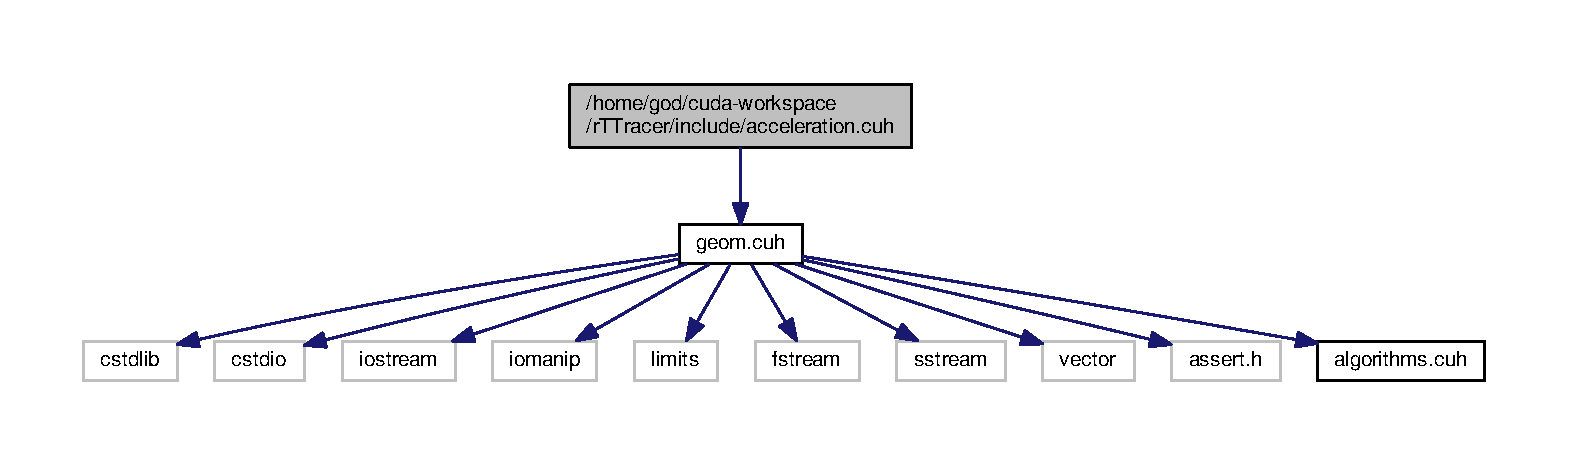
\includegraphics[width=350pt]{acceleration_8cuh__incl}
\end{center}
\end{figure}
\subsection*{Classes}
\begin{DoxyCompactItemize}
\item 
class \hyperlink{class_boundaries}{Boundaries}
\end{DoxyCompactItemize}
\subsection*{Functions}
\begin{DoxyCompactItemize}
\item 
{\footnotesize template$<$class Object\+Type , size\+\_\+t number$>$ }\\class \hyperlink{acceleration_8cuh_a070af818501609893fa3557d5f97d5bb}{\+\_\+\+\_\+align\+\_\+\+\_\+} (16) Dev\+Priority\+Queue\hypertarget{acceleration_8cuh_a070af818501609893fa3557d5f97d5bb}{}\label{acceleration_8cuh_a070af818501609893fa3557d5f97d5bb}

\begin{DoxyCompactList}\small\item\em A priority queue that works on device. Collects pointers to the objects in the painter\textquotesingle{}s algorithm manner. \end{DoxyCompactList}\end{DoxyCompactItemize}


\subsection{Detailed Description}
Kay and Kajiya bounding volumes. 


\hypertarget{algorithms_8cuh}{}\section{/home/god/cuda-\/workspace/r\+T\+Tracer/include/algorithms.cuh File Reference}
\label{algorithms_8cuh}\index{/home/god/cuda-\/workspace/r\+T\+Tracer/include/algorithms.\+cuh@{/home/god/cuda-\/workspace/r\+T\+Tracer/include/algorithms.\+cuh}}
This graph shows which files directly or indirectly include this file\+:
\nopagebreak
\begin{figure}[H]
\begin{center}
\leavevmode
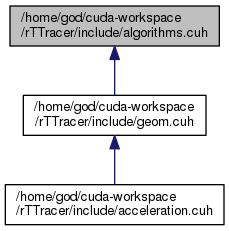
\includegraphics[width=244pt]{algorithms_8cuh__dep__incl}
\end{center}
\end{figure}
\subsection*{Functions}
\begin{DoxyCompactItemize}
\item 
{\footnotesize template$<$typename T $>$ }\\\+\_\+\+\_\+host\+\_\+\+\_\+ \+\_\+\+\_\+device\+\_\+\+\_\+ void \hyperlink{group__auxiliary__algorithms_ga69ab10800d18d0a10396e4acf436f3ef}{algorithms\+::swap} (T \&a, T \&b)
\begin{DoxyCompactList}\small\item\em A device-\/side swap function. \end{DoxyCompactList}\end{DoxyCompactItemize}

\hypertarget{describers_8cuh}{}\section{/home/god/cuda-\/workspace/r\+T\+Tracer/include/describers.cuh File Reference}
\label{describers_8cuh}\index{/home/god/cuda-\/workspace/r\+T\+Tracer/include/describers.\+cuh@{/home/god/cuda-\/workspace/r\+T\+Tracer/include/describers.\+cuh}}
\subsection*{Functions}
\begin{DoxyCompactItemize}
\item 
\+\_\+\+\_\+host\+\_\+\+\_\+ \+\_\+\+\_\+device\+\_\+\+\_\+ bool \hyperlink{group__intersection__test__prperties_gac9af7cfe676f4df793dea5bc53171161}{intersect\+Mesh} (\hyperlink{class_ray}{Ray} \&ray, \hyperlink{class_dev_object}{Dev\+Object} \&obj, \hyperlink{struct_g_p_u_1_1_rendering_context}{G\+P\+U\+::\+Rendering\+Context} \&ctxt)
\begin{DoxyCompactList}\small\item\em Checks if a ray intersects a mesh. \end{DoxyCompactList}\item 
\+\_\+\+\_\+host\+\_\+\+\_\+ \+\_\+\+\_\+device\+\_\+\+\_\+ bool \hyperlink{group__intersection__test__prperties_ga8c05ac13c3cdd49f7e4fa3948cfa4699}{intersect\+Sphere} (\hyperlink{class_ray}{Ray} \&ray, \hyperlink{class_dev_object}{Dev\+Object} \&obj, \hyperlink{struct_g_p_u_1_1_rendering_context}{G\+P\+U\+::\+Rendering\+Context} \&ctxt)
\begin{DoxyCompactList}\small\item\em Checks if a ray intersects a sphere. \end{DoxyCompactList}\item 
\+\_\+\+\_\+host\+\_\+\+\_\+ \+\_\+\+\_\+device\+\_\+\+\_\+ bool \hyperlink{group__intersection__test__prperties_gafbcfd99d540347f9f63d01d6d0b6eef5}{intersect\+Plane} (\hyperlink{class_ray}{Ray} \&ray, \hyperlink{class_dev_object}{Dev\+Object} \&obj, \hyperlink{struct_g_p_u_1_1_rendering_context}{G\+P\+U\+::\+Rendering\+Context} \&ctxt)
\begin{DoxyCompactList}\small\item\em Checks if a ray intersects a plane. \end{DoxyCompactList}\item 
\+\_\+\+\_\+host\+\_\+\+\_\+ \+\_\+\+\_\+device\+\_\+\+\_\+ bool \hyperlink{group__intersection__test__prperties_gae4778d3b0c160c9757d7fca0e5deefa2}{intersect\+Cube} (\hyperlink{class_ray}{Ray} \&ray, \hyperlink{class_dev_object}{Dev\+Object} \&obj, \hyperlink{struct_g_p_u_1_1_rendering_context}{G\+P\+U\+::\+Rendering\+Context} \&ctxt)
\begin{DoxyCompactList}\small\item\em Checks if a ray intersects a cube. \end{DoxyCompactList}\item 
\+\_\+\+\_\+host\+\_\+\+\_\+ \+\_\+\+\_\+device\+\_\+\+\_\+ bool \hyperlink{group__intersection__test__prperties_gaf6bbee9e8a6ee564017fa94cd9e6ec63}{intersect\+Bounding\+Volume} (\hyperlink{class_ray}{Ray} \&ray, float(\&precompute)\mbox{[}2\mbox{]}\mbox{[}7\mbox{]}, \hyperlink{class_dev_object}{Dev\+Object} \&current\+Object, uint8\+\_\+t \&normal\+Index)
\begin{DoxyCompactList}\small\item\em Checks if a ray intersects a bounding slabs of a triangle mesh. \end{DoxyCompactList}\item 
\+\_\+\+\_\+host\+\_\+\+\_\+ \+\_\+\+\_\+device\+\_\+\+\_\+ void \hyperlink{group__intersection__test__prperties_gaa26e85d7aac46c25d6a1b975423f968d}{mesh\+Properties} (const \hyperlink{class_dev_object}{Dev\+Object} \&object, const \hyperlink{class_vec3}{Vec3f} \&hit\+Point, \hyperlink{struct_g_p_u_1_1_rendering_context}{G\+P\+U\+::\+Rendering\+Context} \&ctx, \hyperlink{class_vec2}{Vec2f} \&hit\+Texture\+Coordinates)
\begin{DoxyCompactList}\small\item\em Gets mesh properties on a hitpoint. \end{DoxyCompactList}\item 
\+\_\+\+\_\+host\+\_\+\+\_\+ \+\_\+\+\_\+device\+\_\+\+\_\+ void \hyperlink{group__intersection__test__prperties_gae821d5671069271f7c39d22ca8950f3d}{sphere\+Properties} (const \hyperlink{class_dev_object}{Dev\+Object} \&object, const \hyperlink{class_vec3}{Vec3f} \&hit\+Point, \hyperlink{struct_g_p_u_1_1_rendering_context}{G\+P\+U\+::\+Rendering\+Context} \&ctx, \hyperlink{class_vec2}{Vec2f} \&hit\+Texture\+Coordinates)
\begin{DoxyCompactList}\small\item\em Gets sphere properties on a hitpoint. \end{DoxyCompactList}\item 
\+\_\+\+\_\+host\+\_\+\+\_\+ \+\_\+\+\_\+device\+\_\+\+\_\+ void \hyperlink{group__intersection__test__prperties_gae25700b3104d615db9d575d086c3d994}{plane\+Properties} (const \hyperlink{class_dev_object}{Dev\+Object} \&object, const \hyperlink{class_vec3}{Vec3f} \&hit\+Point, \hyperlink{struct_g_p_u_1_1_rendering_context}{G\+P\+U\+::\+Rendering\+Context} \&ctx, \hyperlink{class_vec2}{Vec2f} \&hit\+Texture\+Coordinates)
\begin{DoxyCompactList}\small\item\em Gets plane properties on a hitpoint. \end{DoxyCompactList}\item 
\+\_\+\+\_\+host\+\_\+\+\_\+ \+\_\+\+\_\+device\+\_\+\+\_\+ void \hyperlink{group__intersection__test__prperties_ga33e6e14712999e0675085b5479201656}{cube\+Properties} (const \hyperlink{class_dev_object}{Dev\+Object} \&object, const \hyperlink{class_vec3}{Vec3f} \&hit\+Point, \hyperlink{struct_g_p_u_1_1_rendering_context}{G\+P\+U\+::\+Rendering\+Context} \&ctx, \hyperlink{class_vec2}{Vec2f} \&hit\+Texture\+Coordinates)
\begin{DoxyCompactList}\small\item\em Gets cube properties on a hitpoint. \end{DoxyCompactList}\item 
void \hyperlink{group__intersection__test__prperties_gae4e3caaa9b4a37b20a8a6f84d0c326aa}{delete\+Mesh} (\hyperlink{class_dev_object}{Dev\+Object} $\ast$object)
\begin{DoxyCompactList}\small\item\em Device memory deallocation function. \end{DoxyCompactList}\item 
\+\_\+\+\_\+device\+\_\+\+\_\+ void \hyperlink{group__intersection__test__prperties_ga4b2a399a49c34312c8369f54b79230af}{transform\+Mesh} (\hyperlink{class_dev_object}{Dev\+Object} $\ast$object, const \hyperlink{class_square_matrix4}{Square\+Matrix4f} \&m\+Transform)
\begin{DoxyCompactList}\small\item\em Whole mesh translation, rotation and scale function. \end{DoxyCompactList}\item 
\+\_\+\+\_\+device\+\_\+\+\_\+ void \hyperlink{group__intersection__test__prperties_ga6fe7123c4c4bdf775eac1231bc37c490}{transform\+Sphere} (\hyperlink{class_dev_object}{Dev\+Object} $\ast$object, const \hyperlink{class_square_matrix4}{Square\+Matrix4f} \&m\+Transform)
\begin{DoxyCompactList}\small\item\em Implicit sphere translation, rotation and scale function. \end{DoxyCompactList}\item 
\+\_\+\+\_\+device\+\_\+\+\_\+ void \hyperlink{group__intersection__test__prperties_ga6d2ae68047e8f8d11a64b9dc9dda507d}{transform\+Plane} (\hyperlink{class_dev_object}{Dev\+Object} $\ast$object, const \hyperlink{class_square_matrix4}{Square\+Matrix4f} \&m\+Transform)
\begin{DoxyCompactList}\small\item\em Implicit sphere translation, rotation and scale function. \end{DoxyCompactList}\item 
\+\_\+\+\_\+device\+\_\+\+\_\+ void \hyperlink{group__intersection__test__prperties_ga00e56ff810e7ba397e903acf50626b55}{transform\+Cube} (\hyperlink{class_dev_object}{Dev\+Object} $\ast$object, const \hyperlink{class_square_matrix4}{Square\+Matrix4f} \&m\+Transform)
\begin{DoxyCompactList}\small\item\em Implicit sphere translation, rotation and scale function. \end{DoxyCompactList}\item 
\+\_\+\+\_\+device\+\_\+\+\_\+ \hyperlink{class_vec3}{Vec3f} \hyperlink{group__intersection__test__prperties_ga19abb6bc50199d8583aafedd0e044b7e}{distant\+Light\+Reflected\+Color} (const \hyperlink{class_i_light}{I\+Light} $\ast$\+\_\+light, \hyperlink{struct_g_p_u_1_1_rendering_context}{G\+P\+U\+::\+Rendering\+Context} \&rctx, \hyperlink{class_vec3}{Vec3f} \&albedo)
\begin{DoxyCompactList}\small\item\em \hyperlink{struct_appearence}{Appearence} of incident light. \end{DoxyCompactList}\item 
\+\_\+\+\_\+device\+\_\+\+\_\+ void \hyperlink{group__intersection__test__prperties_ga6a438778f6ed8683785d7a892a05d312}{illuminate\+Distant} (const \hyperlink{class_i_light}{I\+Light} \&light, const \hyperlink{class_vec3}{Vec3f} \&P, \hyperlink{class_vec3}{Vec3f} \&light\+Dir, \hyperlink{class_vec3}{Vec3f} \&light\+Intensity, float \&distance)
\begin{DoxyCompactList}\small\item\em Implicit sphere translation, rotation and scale function. \end{DoxyCompactList}\item 
\+\_\+\+\_\+device\+\_\+\+\_\+ void \hyperlink{group__intersection__test__prperties_gab3c663df5b5a29d04083e7793bce50d5}{illuminate\+Point} (const \hyperlink{class_i_light}{I\+Light} \&light, const \hyperlink{class_vec3}{Vec3f} \&P, \hyperlink{class_vec3}{Vec3f} \&light\+Dir, \hyperlink{class_vec3}{Vec3f} \&light\+Intensity, float \&distance)
\begin{DoxyCompactList}\small\item\em Implicit sphere translation, rotation and scale function. \end{DoxyCompactList}\item 
void \hyperlink{group__intersection__test__prperties_ga672ecbee3aea2f5567ad7a2611feef3e}{set\+Mesh\+Acceleration\+Volume} (const \hyperlink{class_dev_object}{Dev\+Object} $\ast$current\+Object, \hyperlink{class_boundaries}{Boundaries} $\ast$boundaries, \hyperlink{class_vec3}{Vec3f}(\&bounding\+Plane\+Normals)\mbox{[}7\mbox{]}, float $\ast$(\&gpu\+\_\+all\+Dot\+Products)\mbox{[}7\mbox{]})
\begin{DoxyCompactList}\small\item\em The function gets bounding volume distances computed. \end{DoxyCompactList}\item 
void \hyperlink{group__intersection__test__prperties_gafd2f15ce4a55fb0d8daee0bff024b67b}{set\+Sphere\+Acceleration\+Volume} (const \hyperlink{class_dev_object}{Dev\+Object} $\ast$current\+Object, \hyperlink{class_boundaries}{Boundaries} $\ast$boundaries, \hyperlink{class_vec3}{Vec3f}(\&bounding\+Plane\+Normals)\mbox{[}7\mbox{]}, float $\ast$(\&gpu\+\_\+all\+Dot\+Products)\mbox{[}7\mbox{]})
\begin{DoxyCompactList}\small\item\em The function gets bounding volume distances computed. \end{DoxyCompactList}\item 
void \hyperlink{group__intersection__test__prperties_ga684f41eb2add27e32a7c0115cdd6cce1}{set\+Plane\+Acceleration\+Volume} (const \hyperlink{class_dev_object}{Dev\+Object} $\ast$current\+Object, \hyperlink{class_boundaries}{Boundaries} $\ast$boundaries, \hyperlink{class_vec3}{Vec3f}(\&bounding\+Plane\+Normals)\mbox{[}7\mbox{]}, float $\ast$(\&gpu\+\_\+all\+Dot\+Products)\mbox{[}7\mbox{]})
\begin{DoxyCompactList}\small\item\em The function gets bounding volume distances computed. \end{DoxyCompactList}\item 
void \hyperlink{group__intersection__test__prperties_gabfac85fdf9d0cceb70aefa4c2ed71ad2}{set\+Cube\+Acceleration\+Volume} (const \hyperlink{class_dev_object}{Dev\+Object} $\ast$current\+Object, \hyperlink{class_boundaries}{Boundaries} $\ast$boundaries, \hyperlink{class_vec3}{Vec3f}(\&bounding\+Plane\+Normals)\mbox{[}7\mbox{]}, float $\ast$(\&gpu\+\_\+all\+Dot\+Products)\mbox{[}7\mbox{]})
\begin{DoxyCompactList}\small\item\em The function gets bounding volume distances computed. \end{DoxyCompactList}\item 
\+\_\+\+\_\+device\+\_\+\+\_\+ float \hyperlink{group__intersection__test__prperties_gae0b690ff7b5f9b93e53bb0c1437fbf55}{strips} (const \hyperlink{class_vec2}{Vec2f} \&hit\+Tex\+Coordinates)
\begin{DoxyCompactList}\small\item\em Computes pattern at a particular point in texture. \end{DoxyCompactList}\item 
\+\_\+\+\_\+device\+\_\+\+\_\+ float \hyperlink{group__intersection__test__prperties_gaff97add1678535636b1f4f1ca3f7a96c}{wave} (const \hyperlink{class_vec2}{Vec2f} \&hit\+Tex\+Coordinates)
\begin{DoxyCompactList}\small\item\em Computes pattern at a particular point in texture. \end{DoxyCompactList}\item 
\+\_\+\+\_\+device\+\_\+\+\_\+ float \hyperlink{group__intersection__test__prperties_ga4db329f1c6b211cd0ac9e6dc297f279e}{grid} (const \hyperlink{class_vec2}{Vec2f} \&hit\+Tex\+Coordinates)
\begin{DoxyCompactList}\small\item\em Computes pattern at a particular point in texture. \end{DoxyCompactList}\item 
\+\_\+\+\_\+device\+\_\+\+\_\+ float \hyperlink{group__intersection__test__prperties_ga100df37360dfe6954f51431bc6343dc6}{checker} (const \hyperlink{class_vec2}{Vec2f} \&hit\+Tex\+Coordinates)
\begin{DoxyCompactList}\small\item\em Computes pattern at a particular point in texture. \end{DoxyCompactList}\item 
\+\_\+\+\_\+device\+\_\+\+\_\+ float \hyperlink{group__intersection__test__prperties_ga6ea9f9e6624268a263962a17c6634feb}{none} (const \hyperlink{class_vec2}{Vec2f} \&hit\+Tex\+Coordinates)
\begin{DoxyCompactList}\small\item\em Function just for capability with pattern calculation. \end{DoxyCompactList}\item 
\hyperlink{class_mesh}{Mesh} $\ast$ \hyperlink{describers_8cuh_a09abce6ef7627cd5b34c4074e99be6ce}{load\+Mesh} (std\+::string filename, const \hyperlink{class_square_matrix4}{Square\+Matrix4f} \&model)
\begin{DoxyCompactList}\small\item\em Function to load and transform mesh. \end{DoxyCompactList}\end{DoxyCompactItemize}


\subsection{Function Documentation}
\index{describers.\+cuh@{describers.\+cuh}!load\+Mesh@{load\+Mesh}}
\index{load\+Mesh@{load\+Mesh}!describers.\+cuh@{describers.\+cuh}}
\subsubsection[{\texorpdfstring{load\+Mesh(std\+::string filename, const Square\+Matrix4f \&model)}{loadMesh(std::string filename, const SquareMatrix4f \&model)}}]{\setlength{\rightskip}{0pt plus 5cm}{\bf Mesh} $\ast$ load\+Mesh (
\begin{DoxyParamCaption}
\item[{std\+::string}]{filename, }
\item[{const {\bf Square\+Matrix4f} \&}]{model}
\end{DoxyParamCaption}
)}\hypertarget{describers_8cuh_a09abce6ef7627cd5b34c4074e99be6ce}{}\label{describers_8cuh_a09abce6ef7627cd5b34c4074e99be6ce}


Function to load and transform mesh. 


\begin{DoxyParams}[1]{Parameters}
\mbox{\tt in}  & {\em filename} & -\/ file with a mesh \\
\hline
\mbox{\tt in}  & {\em model} & -\/ object-\/to-\/world matrix \\
\hline
\end{DoxyParams}

\hypertarget{geom_8cuh}{}\section{/home/god/cuda-\/workspace/r\+T\+Tracer/include/geom.cuh File Reference}
\label{geom_8cuh}\index{/home/god/cuda-\/workspace/r\+T\+Tracer/include/geom.\+cuh@{/home/god/cuda-\/workspace/r\+T\+Tracer/include/geom.\+cuh}}
{\ttfamily \#include $<$cstdlib$>$}\\*
{\ttfamily \#include $<$cstdio$>$}\\*
{\ttfamily \#include $<$iostream$>$}\\*
{\ttfamily \#include $<$iomanip$>$}\\*
{\ttfamily \#include $<$limits$>$}\\*
{\ttfamily \#include $<$fstream$>$}\\*
{\ttfamily \#include $<$sstream$>$}\\*
{\ttfamily \#include $<$vector$>$}\\*
{\ttfamily \#include $<$assert.\+h$>$}\\*
{\ttfamily \#include \char`\"{}global\+\_\+constants.\+cuh\char`\"{}}\\*
{\ttfamily \#include \char`\"{}algorithms.\+cuh\char`\"{}}\\*
{\ttfamily \#include \char`\"{}helper.\+cuh\char`\"{}}\\*
Include dependency graph for geom.\+cuh\+:
\nopagebreak
\begin{figure}[H]
\begin{center}
\leavevmode
\includegraphics[width=350pt]{geom_8cuh__incl}
\end{center}
\end{figure}
This graph shows which files directly or indirectly include this file\+:
\nopagebreak
\begin{figure}[H]
\begin{center}
\leavevmode
\includegraphics[width=244pt]{geom_8cuh__dep__incl}
\end{center}
\end{figure}
\subsection*{Classes}
\begin{DoxyCompactItemize}
\item 
class \hyperlink{class_color}{Color}
\item 
class \hyperlink{class_vec2}{Vec2}
\item 
class \hyperlink{class_vec3}{Vec3}
\item 
class \hyperlink{class_square_matrix4}{Square\+Matrix4$<$ T $>$}
\item 
class \hyperlink{class_ray}{Ray}
\item 
struct \hyperlink{struct_camera}{Camera}
\item 
class \hyperlink{class_quaternion}{Quaternion}
\item 
class \hyperlink{class_triangle}{Triangle}
\item 
struct \hyperlink{struct_g_p_u_1_1_rendering_context}{G\+P\+U\+::\+Rendering\+Context}
\item 
struct \hyperlink{struct_vertex_properties}{Vertex\+Properties}
\begin{DoxyCompactList}\small\item\em auxiliary class for .obj files parsing. \end{DoxyCompactList}\end{DoxyCompactItemize}
\subsection*{Typedefs}
\begin{DoxyCompactItemize}
\item 
typedef \hyperlink{class_vec3}{Vec3} {\bfseries Vec3f}
\item 
typedef \hyperlink{class_vec2}{Vec2} {\bfseries Vec2f}
\item 
typedef \hyperlink{class_square_matrix4}{Square\+Matrix4}$<$ float $>$ {\bfseries Square\+Matrix4f}
\end{DoxyCompactItemize}
\subsection*{Enumerations}
\begin{DoxyCompactItemize}
\item 
enum {\bfseries Ray\+Type} \{ {\bfseries P\+R\+I\+M\+A\+R\+Y\+\_\+\+R\+AY}, 
{\bfseries S\+H\+A\+D\+O\+W\+\_\+\+R\+AY}
 \}\hypertarget{group__linear__algebra_ga1d5111b9fffd76014406e866c8784459}{}\label{group__linear__algebra_ga1d5111b9fffd76014406e866c8784459}

\end{DoxyCompactItemize}
\subsection*{Functions}
\begin{DoxyCompactItemize}
\item 
\+\_\+\+\_\+host\+\_\+\+\_\+ \+\_\+\+\_\+device\+\_\+\+\_\+ float {\bfseries clamp} (const float \&lo, const float \&hi, const float \&v)
\item 
constexpr double {\bfseries To\+Radian} (float x)
\item 
\+\_\+\+\_\+host\+\_\+\+\_\+ \+\_\+\+\_\+device\+\_\+\+\_\+ float {\bfseries deg2rad} (const float \&deg)
\item 
\+\_\+\+\_\+host\+\_\+\+\_\+ \+\_\+\+\_\+device\+\_\+\+\_\+ \hyperlink{class_quaternion}{Quaternion} {\bfseries operator$\ast$} (const \hyperlink{class_quaternion}{Quaternion} \&l, const \hyperlink{class_quaternion}{Quaternion} \&r)
\item 
\+\_\+\+\_\+host\+\_\+\+\_\+ \+\_\+\+\_\+device\+\_\+\+\_\+ \hyperlink{class_quaternion}{Quaternion} {\bfseries operator$\ast$} (const \hyperlink{class_quaternion}{Quaternion} \&q, const \hyperlink{class_vec3}{Vec3f} \&v)
\item 
\hyperlink{class_square_matrix4}{Square\+Matrix4f} {\bfseries scale} (float x, float y, float z)
\item 
\hyperlink{class_square_matrix4}{Square\+Matrix4f} {\bfseries translate} (float x, float y, float z)
\item 
\hyperlink{class_square_matrix4}{Square\+Matrix4f} \hyperlink{group__linear__algebra_gac7b995c759cd539cf455cae62c4184e6}{rotate} (const \hyperlink{class_vec3}{Vec3f} \&axis, float deg\+Angle)
\item 
\+\_\+\+\_\+host\+\_\+\+\_\+ \+\_\+\+\_\+device\+\_\+\+\_\+ \hyperlink{class_vec3}{Vec3f} \hyperlink{group__linear__algebra_gaabecdc3e2c4f70f7330aaa6eae1300ac}{refract} (const \hyperlink{class_vec3}{Vec3f} \&incident, const \hyperlink{class_vec3}{Vec3f} \&normal, const float \&refarction\+Index)
\begin{DoxyCompactList}\small\item\em Refraction computation. \end{DoxyCompactList}\item 
\+\_\+\+\_\+host\+\_\+\+\_\+ \+\_\+\+\_\+device\+\_\+\+\_\+ void \hyperlink{group__linear__algebra_ga02c442d21d81c8d0cf889f830eddc236}{fresnel} (const \hyperlink{class_vec3}{Vec3f} \&incident, const \hyperlink{class_vec3}{Vec3f} \&normal, const float \&refraction\+Index, float \&kr)
\begin{DoxyCompactList}\small\item\em amount of reflected and refracted light computation  computes the ratio between two waves\+: parallel and perpendicular polarised light \end{DoxyCompactList}\item 
\+\_\+\+\_\+host\+\_\+\+\_\+ \+\_\+\+\_\+device\+\_\+\+\_\+ float {\bfseries height} (const \hyperlink{class_vec3}{Vec3f} \&top, const \hyperlink{class_vec3}{Vec3f} \&left, const \hyperlink{class_vec3}{Vec3f} \&right)
\item 
\+\_\+\+\_\+host\+\_\+\+\_\+ \+\_\+\+\_\+device\+\_\+\+\_\+ \hyperlink{class_vec3}{Vec3f} \hyperlink{group__linear__algebra_gac9237c364274b9a0fbb9184fae573357}{spiral} (const float \&t, const float \&R, const float \&S)
\item 
void {\bfseries set\+Color\+And\+Texture} (\hyperlink{class_vec3}{Vec3f} \&object\+Color, \hyperlink{class_vec3}{Vec3f} \&texture\+Color, std\+::string \&texturing)
\end{DoxyCompactItemize}
\subsection*{Variables}
\begin{DoxyCompactItemize}
\item 
constexpr float {\bfseries k\+Epsilon} = 1e-\/8
\end{DoxyCompactItemize}

\hypertarget{rendering_8cuh}{}\section{/home/god/cuda-\/workspace/r\+T\+Tracer/include/rendering.cuh File Reference}
\label{rendering_8cuh}\index{/home/god/cuda-\/workspace/r\+T\+Tracer/include/rendering.\+cuh@{/home/god/cuda-\/workspace/r\+T\+Tracer/include/rendering.\+cuh}}


Rendering. Backward ray tracing.  


{\ttfamily \#include \char`\"{}transformations.\+cuh\char`\"{}}\\*
{\ttfamily \#include \char`\"{}thrust\+Helper.\+cuh\char`\"{}}\\*
{\ttfamily \#include $<$omp.\+h$>$}\\*
Include dependency graph for rendering.\+cuh\+:
\nopagebreak
\begin{figure}[H]
\begin{center}
\leavevmode
\includegraphics[width=232pt]{rendering_8cuh__incl}
\end{center}
\end{figure}
This graph shows which files directly or indirectly include this file\+:
\nopagebreak
\begin{figure}[H]
\begin{center}
\leavevmode
\includegraphics[width=232pt]{rendering_8cuh__dep__incl}
\end{center}
\end{figure}
\subsection*{Functions}
\begin{DoxyCompactItemize}
\item 
void $\ast$ {\bfseries G\+P\+U\+::launch\+Asynch\+Ray\+Tracing} (\hyperlink{struct_camera}{Camera} cam, \hyperlink{class_object_box}{Object\+Box} \&objects, unsigned char $\ast$dev\+\_\+bitmap, dim3 \&blocks\+Per\+Grid, dim3 \&threads\+Per\+Block)
\item 
void \hyperlink{group__rendering_gadd1c99922e3b5c249fac22f8946b5e57}{G\+P\+U\+::render} (\hyperlink{struct_camera}{Camera} \&cam, \hyperlink{class_object_box}{Object\+Box} \&objects, unsigned char $\ast$buffer)
\begin{DoxyCompactList}\small\item\em A device kernel launcher. \end{DoxyCompactList}\item 
\+\_\+\+\_\+device\+\_\+\+\_\+ bool {\bfseries G\+P\+U\+::trace} (\hyperlink{class_ray}{Ray} \&ray, \hyperlink{class_object_box}{Object\+Box} \&objects, Rendering\+Context \&rctx, \hyperlink{class_dev_object}{Dev\+Object} $\ast$$\ast$hit\+Object, Ray\+Type raytype=P\+R\+I\+M\+A\+R\+Y\+\_\+\+R\+AY)
\item 
\+\_\+\+\_\+device\+\_\+\+\_\+ \hyperlink{class_vec3}{Vec3f} {\bfseries G\+P\+U\+::shade} (\hyperlink{class_ray}{Ray} \&ray, \hyperlink{class_object_box}{Object\+Box} \&obj, const \hyperlink{struct_camera}{Camera} \&options)
\item 
{\footnotesize template$<$class Bounding\+Volume\+Type , class Distances , size\+\_\+t size$>$ }\\\+\_\+\+\_\+global\+\_\+\+\_\+ void {\bfseries G\+P\+U\+::assign\+Bounding\+Object} (Bounding\+Volume\+Type $\ast$bv, Distances near\+Far\+Distances, size\+\_\+t \+\_\+size=size)\hypertarget{rendering_8cuh_a81d1631d860fe534326c9dcb30d1c2ec}{}\label{rendering_8cuh_a81d1631d860fe534326c9dcb30d1c2ec}

\item 
{\footnotesize template$<$class Object\+Type $>$ }\\\+\_\+\+\_\+global\+\_\+\+\_\+ void {\bfseries G\+P\+U\+::get\+Points} (const Object\+Type $\ast$object, float $\ast$points, size\+\_\+t num)\hypertarget{rendering_8cuh_ae20d656e78c761dae4199fd9e7a547be}{}\label{rendering_8cuh_ae20d656e78c761dae4199fd9e7a547be}

\item 
{\footnotesize template$<$class Object\+Type $>$ }\\\+\_\+\+\_\+global\+\_\+\+\_\+ void {\bfseries G\+P\+U\+::massive\+Dot\+Product} (const Object\+Type $\ast$object, const \hyperlink{class_vec3}{Vec3f} \+\_\+bounding\+Normal, float $\ast$\+\_\+res, size\+\_\+t res\+Len)\hypertarget{rendering_8cuh_a25d7b057a4233ea0016c486e951f7946}{}\label{rendering_8cuh_a25d7b057a4233ea0016c486e951f7946}

\item 
\+\_\+\+\_\+device\+\_\+\+\_\+ bool {\bfseries G\+P\+U\+::is\+Point\+Visible} (\hyperlink{class_object_box}{Object\+Box} \&obj, const uint8\+\_\+t \&light\+Number, const \hyperlink{class_vec3}{Vec3f} \&hit\+Point, Rendering\+Context \&rctx, const float \&bias=0.\+00001f)\hypertarget{rendering_8cuh_adcb3e0c7119489d0f49d385c771df604}{}\label{rendering_8cuh_adcb3e0c7119489d0f49d385c771df604}

\item 
\+\_\+\+\_\+global\+\_\+\+\_\+ void {\bfseries raytracer} (\hyperlink{struct_camera}{Camera} cam, \hyperlink{class_object_box}{Object\+Box} objects, unsigned char $\ast$dev\+\_\+bitmap)
\end{DoxyCompactItemize}


\subsection{Detailed Description}
Rendering. Backward ray tracing. 


\hypertarget{describers_8cu}{}\section{/home/god/cuda-\/workspace/r\+T\+Tracer/source/describers.cu File Reference}
\label{describers_8cu}\index{/home/god/cuda-\/workspace/r\+T\+Tracer/source/describers.\+cu@{/home/god/cuda-\/workspace/r\+T\+Tracer/source/describers.\+cu}}
{\ttfamily \#include \char`\"{}object\+Box.\+cuh\char`\"{}}\\*
{\ttfamily \#include \char`\"{}rendering.\+cuh\char`\"{}}\\*
{\ttfamily \#include \char`\"{}global\+\_\+constants.\+cuh\char`\"{}}\\*
Include dependency graph for describers.\+cu\+:
\nopagebreak
\begin{figure}[H]
\begin{center}
\leavevmode
\includegraphics[width=230pt]{describers_8cu__incl}
\end{center}
\end{figure}
\subsection*{Functions}
\begin{DoxyCompactItemize}
\item 
void \hyperlink{group__intersection__test__prperties_gae4e3caaa9b4a37b20a8a6f84d0c326aa}{delete\+Mesh} (\hyperlink{class_dev_object}{Dev\+Object} $\ast$object)
\begin{DoxyCompactList}\small\item\em Device memory deallocation function. \end{DoxyCompactList}\item 
\+\_\+\+\_\+host\+\_\+\+\_\+ \+\_\+\+\_\+device\+\_\+\+\_\+ bool \hyperlink{group__intersection__test__prperties_gac9af7cfe676f4df793dea5bc53171161}{intersect\+Mesh} (\hyperlink{class_ray}{Ray} \&ray, \hyperlink{class_dev_object}{Dev\+Object} \&obj, \hyperlink{struct_g_p_u_1_1_rendering_context}{G\+P\+U\+::\+Rendering\+Context} \&ctxt)
\begin{DoxyCompactList}\small\item\em Checks if a ray intersects a mesh. \end{DoxyCompactList}\item 
\+\_\+\+\_\+host\+\_\+\+\_\+ \+\_\+\+\_\+device\+\_\+\+\_\+ bool \hyperlink{group__intersection__test__prperties_ga8c05ac13c3cdd49f7e4fa3948cfa4699}{intersect\+Sphere} (\hyperlink{class_ray}{Ray} \&ray, \hyperlink{class_dev_object}{Dev\+Object} \&obj, \hyperlink{struct_g_p_u_1_1_rendering_context}{G\+P\+U\+::\+Rendering\+Context} \&ctxt)
\begin{DoxyCompactList}\small\item\em Checks if a ray intersects a sphere. \end{DoxyCompactList}\item 
\+\_\+\+\_\+host\+\_\+\+\_\+ \+\_\+\+\_\+device\+\_\+\+\_\+ bool {\bfseries plane\+Test} (const \hyperlink{class_plane}{Plane} \&plane, \hyperlink{class_ray}{Ray} \&ray)\hypertarget{describers_8cu_a14459a2c278d18cc5bddc0182a7a1921}{}\label{describers_8cu_a14459a2c278d18cc5bddc0182a7a1921}

\item 
\+\_\+\+\_\+host\+\_\+\+\_\+ \+\_\+\+\_\+device\+\_\+\+\_\+ bool \hyperlink{group__intersection__test__prperties_gafbcfd99d540347f9f63d01d6d0b6eef5}{intersect\+Plane} (\hyperlink{class_ray}{Ray} \&ray, \hyperlink{class_dev_object}{Dev\+Object} \&obj, \hyperlink{struct_g_p_u_1_1_rendering_context}{G\+P\+U\+::\+Rendering\+Context} \&ctxt)
\begin{DoxyCompactList}\small\item\em Checks if a ray intersects a plane. \end{DoxyCompactList}\item 
\+\_\+\+\_\+host\+\_\+\+\_\+ \+\_\+\+\_\+device\+\_\+\+\_\+ bool \hyperlink{group__intersection__test__prperties_gae4778d3b0c160c9757d7fca0e5deefa2}{intersect\+Cube} (\hyperlink{class_ray}{Ray} \&ray, \hyperlink{class_dev_object}{Dev\+Object} \&obj, \hyperlink{struct_g_p_u_1_1_rendering_context}{G\+P\+U\+::\+Rendering\+Context} \&ctxt)
\begin{DoxyCompactList}\small\item\em Checks if a ray intersects a cube. \end{DoxyCompactList}\item 
\+\_\+\+\_\+host\+\_\+\+\_\+ \+\_\+\+\_\+device\+\_\+\+\_\+ bool \hyperlink{group__intersection__test__prperties_gaf6bbee9e8a6ee564017fa94cd9e6ec63}{intersect\+Bounding\+Volume} (\hyperlink{class_ray}{Ray} \&ray, float(\&precompute)\mbox{[}2\mbox{]}\mbox{[}7\mbox{]}, \hyperlink{class_dev_object}{Dev\+Object} \&current\+Object, uint8\+\_\+t \&normal\+Index)
\begin{DoxyCompactList}\small\item\em Checks if a ray intersects a bounding slabs of a triangle mesh. \end{DoxyCompactList}\item 
\+\_\+\+\_\+host\+\_\+\+\_\+ \+\_\+\+\_\+device\+\_\+\+\_\+ void \hyperlink{group__intersection__test__prperties_gaa26e85d7aac46c25d6a1b975423f968d}{mesh\+Properties} (const \hyperlink{class_dev_object}{Dev\+Object} \&object, const \hyperlink{class_vec3}{Vec3f} \&hit\+Point, \hyperlink{struct_g_p_u_1_1_rendering_context}{G\+P\+U\+::\+Rendering\+Context} \&ctx, \hyperlink{class_vec2}{Vec2f} \&hit\+Texture\+Coordinates)
\begin{DoxyCompactList}\small\item\em Gets mesh properties on a hitpoint. \end{DoxyCompactList}\item 
\+\_\+\+\_\+host\+\_\+\+\_\+ \+\_\+\+\_\+device\+\_\+\+\_\+ void \hyperlink{group__intersection__test__prperties_gae821d5671069271f7c39d22ca8950f3d}{sphere\+Properties} (const \hyperlink{class_dev_object}{Dev\+Object} \&object, const \hyperlink{class_vec3}{Vec3f} \&hit\+Point, \hyperlink{struct_g_p_u_1_1_rendering_context}{G\+P\+U\+::\+Rendering\+Context} \&ctx, \hyperlink{class_vec2}{Vec2f} \&hit\+Texture\+Coordinates)
\begin{DoxyCompactList}\small\item\em Gets sphere properties on a hitpoint. \end{DoxyCompactList}\item 
\+\_\+\+\_\+host\+\_\+\+\_\+ \+\_\+\+\_\+device\+\_\+\+\_\+ void {\bfseries get\+Plane\+Properties} (const \hyperlink{class_plane}{Plane} \&plane, const \hyperlink{class_vec3}{Vec3f} \&hit\+Point, \hyperlink{struct_g_p_u_1_1_rendering_context}{G\+P\+U\+::\+Rendering\+Context} \&ctx, \hyperlink{class_vec2}{Vec2f} \&hit\+Texture\+Coordinates)\hypertarget{describers_8cu_a191f45488ebb1c074d20c6c15ca9bab2}{}\label{describers_8cu_a191f45488ebb1c074d20c6c15ca9bab2}

\item 
\+\_\+\+\_\+host\+\_\+\+\_\+ \+\_\+\+\_\+device\+\_\+\+\_\+ void \hyperlink{group__intersection__test__prperties_gae25700b3104d615db9d575d086c3d994}{plane\+Properties} (const \hyperlink{class_dev_object}{Dev\+Object} \&object, const \hyperlink{class_vec3}{Vec3f} \&hit\+Point, \hyperlink{struct_g_p_u_1_1_rendering_context}{G\+P\+U\+::\+Rendering\+Context} \&ctx, \hyperlink{class_vec2}{Vec2f} \&hit\+Texture\+Coordinates)
\begin{DoxyCompactList}\small\item\em Gets plane properties on a hitpoint. \end{DoxyCompactList}\item 
\+\_\+\+\_\+host\+\_\+\+\_\+ \+\_\+\+\_\+device\+\_\+\+\_\+ void \hyperlink{group__intersection__test__prperties_ga33e6e14712999e0675085b5479201656}{cube\+Properties} (const \hyperlink{class_dev_object}{Dev\+Object} \&object, const \hyperlink{class_vec3}{Vec3f} \&hit\+Point, \hyperlink{struct_g_p_u_1_1_rendering_context}{G\+P\+U\+::\+Rendering\+Context} \&ctx, \hyperlink{class_vec2}{Vec2f} \&hit\+Texture\+Coordinates)
\begin{DoxyCompactList}\small\item\em Gets cube properties on a hitpoint. \end{DoxyCompactList}\item 
\+\_\+\+\_\+device\+\_\+\+\_\+ void \hyperlink{group__intersection__test__prperties_ga4b2a399a49c34312c8369f54b79230af}{transform\+Mesh} (\hyperlink{class_dev_object}{Dev\+Object} $\ast$object, const \hyperlink{class_square_matrix4}{Square\+Matrix4f} \&m\+Transform)
\begin{DoxyCompactList}\small\item\em Whole mesh translation, rotation and scale function. \end{DoxyCompactList}\item 
\+\_\+\+\_\+device\+\_\+\+\_\+ void \hyperlink{group__intersection__test__prperties_ga6fe7123c4c4bdf775eac1231bc37c490}{transform\+Sphere} (\hyperlink{class_dev_object}{Dev\+Object} $\ast$object, const \hyperlink{class_square_matrix4}{Square\+Matrix4f} \&m\+Transform)
\begin{DoxyCompactList}\small\item\em Implicit sphere translation, rotation and scale function. \end{DoxyCompactList}\item 
\+\_\+\+\_\+device\+\_\+\+\_\+ void {\bfseries compute\+Plane} (\hyperlink{class_plane}{Plane} \&plane, const \hyperlink{class_square_matrix4}{Square\+Matrix4f} \&m\+Transform)\hypertarget{describers_8cu_a221b492845a6dc62e4e74db676b0d2d1}{}\label{describers_8cu_a221b492845a6dc62e4e74db676b0d2d1}

\item 
\+\_\+\+\_\+device\+\_\+\+\_\+ void \hyperlink{group__intersection__test__prperties_ga6d2ae68047e8f8d11a64b9dc9dda507d}{transform\+Plane} (\hyperlink{class_dev_object}{Dev\+Object} $\ast$object, const \hyperlink{class_square_matrix4}{Square\+Matrix4f} \&m\+Transform)
\begin{DoxyCompactList}\small\item\em Implicit sphere translation, rotation and scale function. \end{DoxyCompactList}\item 
\+\_\+\+\_\+device\+\_\+\+\_\+ void \hyperlink{group__intersection__test__prperties_ga00e56ff810e7ba397e903acf50626b55}{transform\+Cube} (\hyperlink{class_dev_object}{Dev\+Object} $\ast$object, const \hyperlink{class_square_matrix4}{Square\+Matrix4f} \&m\+Transform)
\begin{DoxyCompactList}\small\item\em Implicit sphere translation, rotation and scale function. \end{DoxyCompactList}\item 
\+\_\+\+\_\+device\+\_\+\+\_\+ void \hyperlink{group__intersection__test__prperties_ga6a438778f6ed8683785d7a892a05d312}{illuminate\+Distant} (const \hyperlink{class_i_light}{I\+Light} \&light, const \hyperlink{class_vec3}{Vec3f} \&P, \hyperlink{class_vec3}{Vec3f} \&light\+Dir, \hyperlink{class_vec3}{Vec3f} \&light\+Intensity, float \&distance)
\begin{DoxyCompactList}\small\item\em Implicit sphere translation, rotation and scale function. \end{DoxyCompactList}\item 
\+\_\+\+\_\+device\+\_\+\+\_\+ void \hyperlink{group__intersection__test__prperties_gab3c663df5b5a29d04083e7793bce50d5}{illuminate\+Point} (const \hyperlink{class_i_light}{I\+Light} \&light, const \hyperlink{class_vec3}{Vec3f} \&P, \hyperlink{class_vec3}{Vec3f} \&light\+Dir, \hyperlink{class_vec3}{Vec3f} \&light\+Intensity, float \&distance)
\begin{DoxyCompactList}\small\item\em Implicit sphere translation, rotation and scale function. \end{DoxyCompactList}\item 
\+\_\+\+\_\+device\+\_\+\+\_\+ \hyperlink{class_vec3}{Vec3f} \hyperlink{group__intersection__test__prperties_ga19abb6bc50199d8583aafedd0e044b7e}{distant\+Light\+Reflected\+Color} (const \hyperlink{class_i_light}{I\+Light} $\ast$\+\_\+light, \hyperlink{struct_g_p_u_1_1_rendering_context}{G\+P\+U\+::\+Rendering\+Context} \&rctx, \hyperlink{class_vec3}{Vec3f} \&albedo)
\begin{DoxyCompactList}\small\item\em \hyperlink{struct_appearence}{Appearence} of incident light. \end{DoxyCompactList}\item 
{\footnotesize template$<$class Object\+Type $>$ }\\void \hyperlink{describers_8cu_a62894bfe2e9e2b1cd55216c772eafb27}{set\+Acceleration\+Volume} (const Object\+Type $\ast$object, \hyperlink{class_boundaries}{Boundaries} $\ast$boundaries, \hyperlink{class_vec3}{Vec3f}(\&bounding\+Plane\+Normals)\mbox{[}7\mbox{]}, float $\ast$(\&gpu\+\_\+all\+Dot\+Products)\mbox{[}7\mbox{]})
\begin{DoxyCompactList}\small\item\em The wrapper function gets bounding volume distances computed. \end{DoxyCompactList}\item 
void \hyperlink{group__intersection__test__prperties_ga684f41eb2add27e32a7c0115cdd6cce1}{set\+Plane\+Acceleration\+Volume} (const \hyperlink{class_dev_object}{Dev\+Object} $\ast$current\+Object, \hyperlink{class_boundaries}{Boundaries} $\ast$boundaries, \hyperlink{class_vec3}{Vec3f}(\&bounding\+Plane\+Normals)\mbox{[}7\mbox{]}, float $\ast$(\&gpu\+\_\+all\+Dot\+Products)\mbox{[}7\mbox{]})
\begin{DoxyCompactList}\small\item\em The function gets bounding volume distances computed. \end{DoxyCompactList}\item 
void \hyperlink{group__intersection__test__prperties_gabfac85fdf9d0cceb70aefa4c2ed71ad2}{set\+Cube\+Acceleration\+Volume} (const \hyperlink{class_dev_object}{Dev\+Object} $\ast$current\+Object, \hyperlink{class_boundaries}{Boundaries} $\ast$boundaries, \hyperlink{class_vec3}{Vec3f}(\&bounding\+Plane\+Normals)\mbox{[}7\mbox{]}, float $\ast$(\&gpu\+\_\+all\+Dot\+Products)\mbox{[}7\mbox{]})
\begin{DoxyCompactList}\small\item\em The function gets bounding volume distances computed. \end{DoxyCompactList}\item 
void \hyperlink{group__intersection__test__prperties_ga672ecbee3aea2f5567ad7a2611feef3e}{set\+Mesh\+Acceleration\+Volume} (const \hyperlink{class_dev_object}{Dev\+Object} $\ast$current\+Object, \hyperlink{class_boundaries}{Boundaries} $\ast$boundaries, \hyperlink{class_vec3}{Vec3f}(\&bounding\+Plane\+Normals)\mbox{[}7\mbox{]}, float $\ast$(\&gpu\+\_\+all\+Dot\+Products)\mbox{[}7\mbox{]})
\begin{DoxyCompactList}\small\item\em The function gets bounding volume distances computed. \end{DoxyCompactList}\item 
void \hyperlink{group__intersection__test__prperties_gafd2f15ce4a55fb0d8daee0bff024b67b}{set\+Sphere\+Acceleration\+Volume} (const \hyperlink{class_dev_object}{Dev\+Object} $\ast$current\+Object, \hyperlink{class_boundaries}{Boundaries} $\ast$boundaries, \hyperlink{class_vec3}{Vec3f}(\&bounding\+Plane\+Normals)\mbox{[}7\mbox{]}, float $\ast$(\&gpu\+\_\+all\+Dot\+Products)\mbox{[}7\mbox{]})
\begin{DoxyCompactList}\small\item\em The function gets bounding volume distances computed. \end{DoxyCompactList}\item 
\+\_\+\+\_\+device\+\_\+\+\_\+ float \hyperlink{group__intersection__test__prperties_gae0b690ff7b5f9b93e53bb0c1437fbf55}{strips} (const \hyperlink{class_vec2}{Vec2f} \&hit\+Tex\+Coordinates)
\begin{DoxyCompactList}\small\item\em Computes pattern at a particular point in texture. \end{DoxyCompactList}\item 
\+\_\+\+\_\+device\+\_\+\+\_\+ float \hyperlink{group__intersection__test__prperties_gaff97add1678535636b1f4f1ca3f7a96c}{wave} (const \hyperlink{class_vec2}{Vec2f} \&hit\+Tex\+Coordinates)
\begin{DoxyCompactList}\small\item\em Computes pattern at a particular point in texture. \end{DoxyCompactList}\item 
\+\_\+\+\_\+device\+\_\+\+\_\+ float \hyperlink{group__intersection__test__prperties_ga4db329f1c6b211cd0ac9e6dc297f279e}{grid} (const \hyperlink{class_vec2}{Vec2f} \&hit\+Tex\+Coordinates)
\begin{DoxyCompactList}\small\item\em Computes pattern at a particular point in texture. \end{DoxyCompactList}\item 
\+\_\+\+\_\+device\+\_\+\+\_\+ float \hyperlink{group__intersection__test__prperties_ga100df37360dfe6954f51431bc6343dc6}{checker} (const \hyperlink{class_vec2}{Vec2f} \&hit\+Tex\+Coordinates)
\begin{DoxyCompactList}\small\item\em Computes pattern at a particular point in texture. \end{DoxyCompactList}\item 
\+\_\+\+\_\+device\+\_\+\+\_\+ float \hyperlink{group__intersection__test__prperties_ga6ea9f9e6624268a263962a17c6634feb}{none} (const \hyperlink{class_vec2}{Vec2f} \&hit\+Tex\+Coordinates)
\begin{DoxyCompactList}\small\item\em Function just for capability with pattern calculation. \end{DoxyCompactList}\end{DoxyCompactItemize}


\subsection{Function Documentation}
\index{describers.\+cu@{describers.\+cu}!set\+Acceleration\+Volume@{set\+Acceleration\+Volume}}
\index{set\+Acceleration\+Volume@{set\+Acceleration\+Volume}!describers.\+cu@{describers.\+cu}}
\subsubsection[{\texorpdfstring{set\+Acceleration\+Volume(const Object\+Type $\ast$object, Boundaries $\ast$boundaries, Vec3f(\&bounding\+Plane\+Normals)[7], float $\ast$(\&gpu\+\_\+all\+Dot\+Products)[7])}{setAccelerationVolume(const ObjectType *object, Boundaries *boundaries, Vec3f(\&boundingPlaneNormals)[7], float *(\&gpu\_allDotProducts)[7])}}]{\setlength{\rightskip}{0pt plus 5cm}template$<$class Object\+Type $>$ template$<$ class Object\+Type $>$ void set\+Acceleration\+Volume (
\begin{DoxyParamCaption}
\item[{const Object\+Type $\ast$}]{object, }
\item[{{\bf Boundaries} $\ast$}]{boundaries, }
\item[{{\bf Vec3f}(\&)}]{bounding\+Plane\+Normals\mbox{[}7\mbox{]}, }
\item[{float $\ast$(\&)}]{gpu\+\_\+all\+Dot\+Products\mbox{[}7\mbox{]}}
\end{DoxyParamCaption}
)}\hypertarget{describers_8cu_a62894bfe2e9e2b1cd55216c772eafb27}{}\label{describers_8cu_a62894bfe2e9e2b1cd55216c772eafb27}


The wrapper function gets bounding volume distances computed. 


\begin{DoxyParams}[1]{Parameters}
\mbox{\tt in}  & {\em object} & -\/ wrapper object with pointer to the stored in device memory specific instance. \\
\hline
\mbox{\tt out}  & {\em boundaries} & -\/ to store result \\
\hline
\mbox{\tt in}  & {\em bounding\+Plane\+Normals} & -\/ bounding plane orientation normals. \\
\hline
\mbox{\tt out}  & {\em gpu\+\_\+all\+Dot\+Products} & -\/ allocated in advance device memory to store all possible distances the function uses. \\
\hline
\end{DoxyParams}
\begin{DoxyRefDesc}{Bug}
\item[\hyperlink{bug__bug000001}{Bug}]thrust library allocation causes a bad\+\_\+alloc \end{DoxyRefDesc}

%--- End generated contents ---

% Index
\backmatter
\newpage
\phantomsection
\clearemptydoublepage
\addcontentsline{toc}{chapter}{Index}
\printindex

\end{document}
